% Preamble =========================================================================================
%\input{preamble}

\documentclass[12pt]{article}

\usepackage{lipsum}
\usepackage[margin=1in,left=1in,includefoot]{geometry}
\usepackage{graphicx} %allows for impage import
\graphicspath{{images/}}
\usepackage[hidelinks]{hyper ref} % Allows for clickable links
\usepackage{sectsty}
\usepackage{multirow}
\usepackage{booktabs}
\usepackage[T1]{fontenc}
\usepackage{lmodern}
\usepackage[none]{hyphenat}
\usepackage{array}
\usepackage{lscape}
\usepackage{geometry}
\usepackage{pdflscape}
\usepackage{longtable}
\usepackage[utf8]{inputenc}
\usepackage[english]{babel}
%\usepackage[table]{xcolor}
\usepackage{colortbl}
%\usepackage{fixltx2e}
\usepackage{hhline}
\usepackage{dcolumn}
\usepackage{tocloft}
\setlength{\cftsubsecnumwidth}{3em}
\setlength{\cftsubsubsecnumwidth}{4em}
\usepackage{hyperref}
\hypersetup{pdftex,colorlinks=true,allcolors=black}
\usepackage{hypcap}
\usepackage{amsmath}
\usepackage{hyperref}

\definecolor{lightgray}{gray}{0.92}

\newcolumntype{L}{>{\centering\arraybackslash}m{3in}}

\usepackage{float}
\usepackage{fancyhdr}
\pagestyle{fancy}
\fancyhead{}

\setlength{\extrarowheight}{1.5pt}
\setlength{\arraycolsep}{1.5pt}


\begin{document}
	\begin{titlepage}
			\begin{center}
				\huge{\bfseries Stock Synthesis}\\
				\huge{\bfseries User Manual}\\		
				[0.50in]
				\huge{\bfseries Version 3.30.10}\\
				[1in]
				\LARGE{February 2, 2018}\\
				[1in]
				\LARGE{Richard D. Methot}\\
				%\LARGE{Teresa A'mar}\\
			    \LARGE{Chantel Wetzel}\\
			    \LARGE{Ian Taylor}\\
			    [1in]
				NOAA Fisheries\\
				Seattle, WA USA\\		
			\end{center}
		\end{titlepage}
		
		% ====== Table of Contents ===================================================
		\pagenumbering{roman}
		\tableofcontents
		\thispagestyle{empty}
		\cleardoublepage
		\setcounter{page}{1}
		\newpage
		
		% ====  List of figures ========================================================
		\renewcommand{\headrulewidth}{0pt} % removes the top line across each page
		%\listoffigures
		%\addcontentsline{toc}{section}{\numberline{}List of Figures}
		\cleardoublepage

		% ====== Section 1 - 5 =============================================================
		\pagenumbering{arabic}
		
 \section{Introduction}\label{sec:intro}
 \begin{sloppypar}
This manual provides a guide for using the stock assessment program, Stock Synthesis (SS). The guide contains a description of the input and output files and usage instructions. A technical description of the model itself is in Methot and Wetzel (2013). SS is programmed using Auto Differentiation Model Builder (ADMB; Fournier 2001. ADMB is now available at admb-project.org). SS currently is compiled using ADMB version 11.using various compilers to provide Windows, MacOS and Linux executables. The model and a graphical user interface are available from the NOAA VLAB at https://vlab.ncep.noaa.gov/group/stock-synthesis/home. The VLAB site also provides a user forum for posting Q\&A and for accessing various additional materials.  An output processor package, r4ss, in R is available for download from CRAN or GitHub. Additional information about the package can be located at github.com/r4ss/r4ss.
\end{sloppypar}
	
\section{New Features Available in Version 3.30}
		Stock Synthesis version 3.30 was designed specifically to provide more precise temporal control of growth, expected values for data, and for recruitment.  In additional, a large number of new features that make substantial changes to the input formats have been introduced.  Two versions of SS are provided.  One, sstrans,exe, will read SS3.24 input files and produce SS3.30 formatted versions of those input files.  Nearly every feature in 3.24 can be converted by this program.  The other version, ss.exe, will then be your primary new assessment tool. Additional information on each new feature available by clicking on the "Item".
		
		\begin{center}
			\begin{longtable}{p{2cm} p{3cm} p{10cm}}
				Category & Item & Description\\
				\hline
				\endfirsthead
		
				Category & Item & Description\\
				\hline
				\endhead
		
				\hline
				\endfoot
		
				\endlastfoot
				
				General & 
					\hyperlink{GenericFleets}{Generic Fleets} & 
						Fleet specification section of data file is much changed and now includes fleet type, so fishery fleets, bycatch fleets, surveys, and someday predators are specified in any order\\
				  \\
				  & \hyperlink{ListBased}{List-oriented inputs} & 
					    Rather than specify the number of items to be read, now SS can figure it out on its own with lists terminated by -9999 in first field of the read vector \\
				  \\					  
				  & \hyperlink{SubSeas}{Internal sub-seasons} & 
					    SS v3.24 inherently has 2 subseasons each season (begin and middle) at which the age-length-key (ALK) is calculated; now user specifies an even number of sub-seasons to use (2 to many) \\
				  \\
				  & \hyperlink{ObsTiming}{Observation Timing} & 
					    Timing of observations now is input as year, month where month is real; e.g. April 15 is 4.5; age-length-key (ALK) used for each observation is calculated to the nearest sub-season.  Old "survey\_timing" replaced by the month specific inputs.  Season is calculated at runtime from the input month and the input season durations. \\
				  \\
				  & \hyperlink{ALK}{Speed} & 
					    Smarter at when to re-calculate the age-length-key (ALK); trims tails of size-at-age so calculations avoid many inconsequential cells of the age-length matrix. ALK tail compression is specified in the starter file.\\
				  \\				
				  & \hyperlink{Convert} {Converter} & 
					    Special version of SS, ss\_trans.exe, will read files in 3.24 format and write *.ss\_new files in 3.30 format.  This is the advised method for converting previous version files, but always do a side-by-side comparison.\\
				  \\
				  & \hyperlink{WAAparm} {Empirical Weight-at-Age} & Implementing empirical weight-at-age is now specified separately in the control file rather than under the maturity options.\\
				  \\
				  & \hyperlink{Priors}{Prior Type} & Change in the prior numbering for parameters.  Now, 0 indicates no prior, and 6 indicates a normal distribution prior.\\
				\hline
				Fishery and Catch & 
					\hyperlink{CatchMult}{Catch multiplier} & 
						Each fishing fleet's catch can now have a "q" that is a parameter in the MGparm section.\\
				  \\						
					& \hyperlink{CatchFormat}{Catch input} & 
						Catch input now as list:  yr, seas, fleet, amount, se. \\
				  \\						
					& \hyperlink{CompTiming}{Observations} & 
						Fishery composition observations can be related to season long catch-at-age, or to a month-specific timing.\\
				  \\					
					& \hyperlink{DomeRetention}{Retention} & 
						Option for dome-shaped retention function and for age-based retention. \\
				\hline
				Selectivity 
					& Scaling Options& 	
						A new non-parametric selectivity types that are scaled by the raw values at particular ages, rather than the max age.\\
				%\hline
				Survey
					& Special Survey Types & 
						Special selectivity options (type 30 or $>$) are no longer specified within the control file.  Specifying the use of one of these selectivity types is now done within the data file by selecting the survey "units". \\  
				  \\
					& \hyperlink{Qsetup}{Link functions} & 
						Q\_power is now one of several, and growing, set of link functions. \\
				  \\						
					& \hyperlink{Qsetup}{Catchability setup reorganization} & 
						Major reorganization of catchability (Q) setup, including the link specification. \\
				  \\					
					& \multicolumn{1}{l}{\hyperlink{Qsetup}{Q as a parameter}} & 
						Each survey now must have a Q parameter and its value still can float (as old option 5).\\
				\hline
				Recruitment
					& \hyperlink{Shepard}{Shepard SRR} & 
						A 3-parameter Shepard stock-recruitment curve is now an option.\\
					\\
					& \hyperlink{RecrTiming}{Recruitment timing} & 
						Replace "birthseason" with "settlement event" that has explicit timing offset from spawning.  Month of spawning and each settlement event must be specified and need not be at beginning of a season.\\
				\hline
				Benchmark 
					& Global MSY &  
						Global MSY based on knife edge age selection; also do calculation with single age selection. The global MSY value will automatically be included in the report file.\\
				  \\					
					& Mean recruitment distribution & 
						In multi-area model, can now specify range of years to use for the average recruitment distribution for forecasting. This feature is not yet implemented. \\
				  \\
				\hline
				Forecast & 
					Process error & 
						Propagate random walk in MGparms, catchability, and selectivity into forecast. Specifying the end year for process error in the forecast period will implement this option.  This option has only been partial implemented at this junction and will be completed in later versions.\\
				\hline
				Biology 
					& \hyperlink{MGorder}{Parameter order} & 
						MGparms now have maturity, fecundity, sex ratio, and weight-length by growth pattern.\\
				  \\						
				    & \hyperlink{SexRatio}{Sex ratio} & 
					    Change sex ratio at birth from a constant to a morph-specific MGparameter. \\
				%\hline
				Statistical 
					& \hyperlink{GcompVar}{Input variance adjuster} & 
						Added variance adjustment factor for generalized size comp. \\
				  \\						
					& Deviation vectors & 
						Variance of deviation vectors is now specified with 2 parameters for standard error and auto-correlation (rho), so can be estimated.\\
				  \\						
					& \hyperlink{Dirichlet}{Dirichlet multinomial} & 
						Dirichlet multinomial now a fleet-specific option; takes one parameter per fleet. \\
				\hline
				Parameters 
					& \hyperlink{paraOrder}{Parameter order} & The prior standard deviation column for all parameter lines has been moved before the prior type column.  This modification improves formatting output between integer and decimal inputs.\\ 
				 \\
					& Density dependence & 
						Beginning of year summary biomass and the rec\_dev parameters are mapped to the "environmental" matrix so that parameters can be density-dependent.\\
				  \\						
					& \hyperlink{tvOrder}{Re-order} & 
						Pay attention to the new order of the time-varying adjustments to parameters (block/trend, then environmental, then deviations). \\
				  \\						
					& \hyperlink{time-vary}{Time-varying parameters} & 
						Long parameter lines for spawner-recruit relationship (SRR), catchability (Q), and tag parameters and complete re-vamp of the way that time-varying parameters are implemented for SRR and Q.  Now shares same internal code as mortality-growth and selectivity parameters for time-varying capabilities.\\
				\hline	
			\end{longtable}
		\end{center}
		
\subsection{SS v.3.24 Issues Detected}
The process of updating and adding new features within SS v.3.30 expose several issues with the previous version that have been corrected:
\begin{enumerate}
	\item Recruitment timing in multi-season models: When spawning occurred in a late season one year and recruits occurred at beginning of a season the next year, the recruits were starting at age-0, which was illogical.  SS v.3.30 corrects this so that recruits are age-0 only if recruiting at or between the time of spawning and the end of the year, and recruits after January 1st start at age-0.  A manual option allows users to attempt to replicate the SS v.3.24 protocol.
	\item Lorenzen $M$ and time-varying growth interaction: There needs to be a revision to SS v.3.30 so that growth can be updated each season prior to calculating Lorenzen $M$.
	\item Length at maximum age: SS v.3.24 intended to decay this length over-time at $M + F$ decreased the abundance of fish implicitly older than the maximum age (agemax).  However, this decay was only implemented in years for which time-varying growth was updated.  This will go on the the SS v.3.30 future features wishlist.
\end{enumerate}

		
\section{File Organization}\label{FileOrganization}		
	\subsection{Input Files}
	\begin{enumerate}
		\item starter.ss:   required file containing filenames of the data file and the control file plus other run controls (required).
		\item datafile:  file containing model dimensions and the data (required)
		\item control file:  file containing set-up for the parameters (required)
		\item forecast.ss:  file containing specifications for reference points and forecasts (required) 
		\item ss.par:  previously created parameter file that can be read to overwrite the initial parameter values in the control file (optional)
		\item runnumber.ss:  file containing a single number used as runnumber in output to CumReport.sso and in the processing of profilevalues.ss (optional)
		\item profilevalues.ss:  file contain special conditions for batch file processing (optional)
		item wtatage.ss: file containing empirical input of body weight by fleet and population and empirical fecundity-at-age (optional)
	\end{enumerate}
	
	\subsection{Output Files}
	\begin{enumerate}
		\item ss.par, ss.std, ss.rep, ss.cor etc.  standard ADMB output files
		\item echoinput.sso:  This file is produced while reading the input files and includes an annotated echo of the input.  The sole purpose of this output file is debugging input errors.
		\item warning.sso:  This file contains a list of warnings generated during program execution.
		\item checkup.sso:  Contains details of selectivity parameters and resulting vectors.  This is written during the first call of the objective function.
		\item Report.sso:  This file is the primary report file.
		\item CompReport.sso:  Observed and expected composition data in a list-based format
		\item Forecast-report.sso:  Output of management quantities and for forecasts
		\item CumReport.sso:  This file contains a brief version of the run output, output is appended to current content of file so results of several runs can be collected together.  This is useful when a batch of runs is being processed.
		\item Covar.sso:  This file replaces the standard ADMB ss.cor with an output of the parameter and derived quantity correlations in database format
		\item Gradient.dat: New for SS3.30, this file shows parameter gradients at the end of the run.
		\item data.ss\textunderscore new:  contains a user-specified number of datafiles, generated through a parametric bootstrap procedure, and written sequentially to this file
		\item control.ss\textunderscore new:  Updated version of the control file with final parameter values replacing the Init parameter values.
		\item starter.ss\textunderscore new:  New version of the starter file with annotations
		\item Forecast.ss\textunderscore new:  New version of the forecast file with annotations.
		\item rebuild.dat:  Output formatted for direct input to Andre Punt's rebuilding analysis package.  Cumulative output is output to REBUILD.SS (useful when doing MCMC or profiles).
		\item SIS\_table.sso:  Output formatted for reading into the NMFS Species Information System.
		\item Parmtrace.sso: Parameter values at each iteration.
		\item posteriors.sso, derived\_posteriors.sso, posterior\_vectors.sso: files associated with MCMC.
	\end{enumerate}

	
	\subsection{Auxiliary Files}
	\begin{enumerate}
		\item SSv330-OUTPUT.XLS:   Excel file with macros to read report.sso and display results
		\item SELEX24\textunderscore dbl\textunderscore normal.XLS:
		\begin{enumerate}
			\item This excel file is used to show the shape of a double normal selectivity (option number 20 for age-based and 24 for length-based selectivity) given user-selected parameter values.
			\item Instructions are noted in the XLS file but, to summarize
			\begin{enumerate}
				\item Users should only change entries in a yellow box. 
				\item Parameter values are changed manually or using sliders, depending on the value of cell I5.
			\end{enumerate}
			\item It is recommend that users select plausible starting values for double-normal selectivity options, especially when estimating all 6 parameters
			\item Please note that the XLS does NOT show the impact of setting parameters 5 or 6 to ''-999''.  In SS v3.30, this allows the the value of selectivity at the initial and final age or length to be determined by the shape of the double-normal arising from parameters 1-4, rather than forcing the selectivity at the intial and final age or length to be estimated separately using the value of parameters 5 and 6. 
		\end{enumerate}
		\item SELEX17\textunderscore age\textunderscore randwalk.XLS:
		\begin{enumerate}
			\item This excel file is used to show the shape of age-based selectivity arising from option 17 given user-selected parameter values
			\item Users should only change entries in the yellow box.
			\item The red box is the maximum cumulative value, which is subtracted from all cumulative values.  This is then exponentiated to yield the estimated selectivity curve.  Positive values yield increasing selectivity and negative values yield decreasing selectivity.
		\end{enumerate}
		\item PRIOR-TESTER.XLS:
		\begin{enumerate}
			\item The 'compare' tab of this spreadsheet shows how the various options for defining parameter priors work
		\end{enumerate}
		\item SS-Control\textunderscore Setup.XLS:
		\begin{enumerate}
			\item Shows how to setup an example control file for SS
		\end{enumerate}
		\item SS-Data\textunderscore Input.XLS:
		\begin{enumerate}
			\item Shows how to setup an example data input for SS
		\end{enumerate}
		\item Growth.XLS: 
		\begin{enumerate}
			\item Excel file to test parameterization between the growth curve options within SS.
			\item Instructions are noted in the XLS file but, to summarize
			\begin{enumerate}
				\item Users should only change entries in a yellow box.  
				\item Entries in a red box are used internally, and can be compared with other parameterizations, but should not be changed.
			\end{enumerate}
			\item The SS-VB is identical to the standard VB, but uses a parameterization where length is estimated at pre-defined ages, rather than A=0 and A=Inf.  The Schnute- Richards is identical to the Richards-Maunder, but similarly uses the parameterization with length at pre-defined ages.  The Richards coefficient controls curvature, and if the curvature coefficient = 1, it reverts to the standard VB curve. 
		\end{enumerate}
		\item Movement.XLS:
		\begin{enumerate}
			\item Excel file to explore SS movement parameterization
		\end{enumerate}
	\end{enumerate}
		
\section{Starting SS}
SS is typically run through the command line interface although it can also be called from another program such as R or the SS-GUI or a script file (such as a DOS batch file). SS is compiled for Windows, Mac, and Linux operating systems. The memory requirements depend on the complexity of the model you run, but in general, SS will run much slower on computers with inadequate memory. See the section \ref{RunningSS} for additional notes on methods of running SS.

Communication with the program is through text files.  When the program first starts, it reads the file starter.ss, which typically must be located in the same directory from which SS is being run.  The file starter.ss contains required input information plus references to other required input files, as described in section \ref{FileOrganization}.  The names of the control and data files must match the names specified in the starter.ss file.  File names, including starter.ss, are case-sensitive on Linux and Mac systems but not on Windows. Output from SS is as text files containing specific keywords.  Output processing programs, such as the SS GUI, Excel, or R can search for these keywords and parse the specific information located below that keyword in the text file.


		
		% ======== Section 6: Starter File
		
\section{Starter File}

SS begins by reading the file starter.ss.  Its format and content is as follows.  Note that the term COND in the Typical Value column means that the existence of input shown there is conditional on a value specified earlier in the file.  Omit or comment out these entries if the appropriate condition has not been selected.

{
\setlength\extrarowheight{4pt}
\begin{landscape}

\centerline{\large{STARTER.SS}} 
\vspace{0.1in}
%{\renewcommand{\arraystretch}{1.1}

\begin{longtable}{p{1.5cm} p{7cm} p{12.5cm}} 

 \hline
 \textbf{Value} & \textbf{Options} & \textbf{Description} \TBstrut \\ 
 \hline
 \endfirsthead
 
 \hline
 \textbf{Value} & \textbf{Options} & \textbf{Description} \TBstrut \\ 
 \hline
 \endhead
 
 \hline
 \endfoot
 
 \hline
 \multicolumn{3}{ c }{ \textbf{End of Starter File}}\Tstrut\Bstrut\\
 \hline
 \endlastfoot

 \#C this is a starter comment & Must begin with \#C then rest of the line is free form & All lines in this file beginning with \#C will be retained and written to the top of several output files \Tstrut\\
		
 \hline
 data\textunderscore file.dat &  & File name of the data file \Tstrut\\
		
 \hline
 control\textunderscore file.ctl &  & File name of the control file \Tstrut\\
   
 \hline		
 0 & Initial Parameter Values: & \multirow{1}{1cm}[-0.25cm]{\parbox{12.5cm}{Don't use this if there have been any changes to the control file that would alter the number or order of parameters stored in the ss.par file.  Values in ss.par can be edited, carefully. Do not run sstrans.exe from a ss.par from SS v.3.24.}}\Tstrut\\
 & 0 = use values in control file; &  \\
 & 1 = use ss.par after reading setup in the control file & \\
		
 \hline
 1 & Run display detail: &  \multirow{1}{1cm}[-0.25cm]{\parbox{12.5cm}{With option 2, the display shows value of each -logL component for each iteration and it displays where crash penalties are created}} \Tstrut\\
   & 0 = none other than ADMB outputs; & \\
   & 1 = one brief line of display for each iteration; & \\
   & 2 = fuller display per iteration & \\
		  
 \hline
 1 & Detailed age-structure report & \multirow{1}{1cm}[-0.15cm]{\parbox{12.5cm}{Detailed age-structured report in Report.sso}} \Tstrut\\
   & 0 = minimal (no Report file); & \\
   & 1 = include all output; &  \\
   & 2 = brief output &  \\		 
		 
 \pagebreak%\hline
 0 & Write 1st iteration details & \multirow{1}{1cm}[-0.25cm]{\parbox{12.5cm}{This output is largely unformatted and undocumented and is mostly used by the developer. }} \Tstrut\\
   & 0 = omit & \\
   & 1 = write detailed intermediate calculations to echoinput.sso during first call & \\

 \hline
 0 & Parameter Trace & \multirow{1}{1cm}[-0.25cm]{\parbox{12.5cm}{This controls the output to parmtrace.sso. The contents of this output can be used to determine which values are changing when a model approaches a crash condition.  It also can be used to investigate patterns of parameter changes as model convergence slowly moves along a ridge.}} \Tstrut\\
   & 0 = omit & \\
   & 1 = write good iteration and active parameters & \\
   & 2 = write good iterations and all parameters & \\
   & 3 = write every iteration and all parameters & \\
   & 4 = write every iteration and active parameters &  \\
   
 \hline
 1 & Cumulative Report & \multirow{1}{1cm}[-0.25cm]{\parbox{12.5cm}{Controls reporting to the file Cumreport.sso.
 		This cumulative report is most useful when accumulating summary information from likelihood profiles or when simply accumulating a record of all model runs within the current subdirectory}}\Tstrut\\
   & 0 = omit  & \\
   & 1 = brief & \\
   & 2 = full  &  \\
	 
 \hline
 1 & Full Priors & \multirow{1}{1cm}[-0.25cm]{\parbox{12.5cm}{Turning on this option causes all prior values to be calculated.  With this option off, the total log likelihood, which includes the log likelihood for priors, would change between model phases as more parameters became active.}} \Tstrut\\
   & 0 = only calculate priors for active parameters &	\\
   & 1 = calculate priors for all parameters that have a defined prior & \\
	     
 %\hline
 \pagebreak
 1 & Soft Bounds & \multirow{1}{1cm}[-0.25cm]{\parbox{12.5cm}{This option creates a weak symmetric beta penalty for the selectivity parameters.  This becomes important when estimating selectivity functions in which the values of some parameters cause other parameters to have negligible gradients, or when bounds have been set too widely such that a parameter drifts into a region in which it has negligible gradient.  The soft bound creates a weak penalty to move parameters away from the bounds.}} \Tstrut\\
   & 0 = omit & \\
   & 1 = use & \\
   & & \\
   & & \\
   & & \\

 
 \hline
 1 & Data File Output & \multirow{1}{1cm}[-0.25cm]{\parbox{12.5cm}{All output files are sequentially output to data.ss\_new and will need to be parsed by the user into separate data files. The output of the input data file makes no changes, so retains the order of the original file. Output files 2-N contain only observations that have not been excluded through use of the negative year denotation, and the order of these output observations is as processed by the model. The N obs values are adjusted accordingly.  At this time, the tag recapture data is not output to DATA.SS\textunderscore new.}}\Tstrut\\
   & 0 = none & \\
   & 1 = output an annotated replicate of the input data file & \\
   & 2 = add a second data file containing the model's expected values with no added error & \\
   & 3+ = add N-2 parametric bootstrap data files & \\

 \hline
 8 & Turn off estimation &  \multirow{1}{1cm}[-0.25cm]{\parbox{12.5cm}{The 0 option is useful for (1) quickly reading in a messy set of input files and producing the annotated control.ss\_new and data.ss\_new files, or (2) examining model output based solely on input parameter values.  Similarly, the value option allows examination of model output after completing a specified phase.  Also see usage note for restarting from a specified phase.}}\Tstrut\\
   & -1 = exit after reading input files & \\
   & 0 = exit after one call to the calculation routines and production of sso and ss\_new files & \\
   & <positive value> = exit after completing this phase & \\	  
	     
 \hline
 10 & MCMC burn interval & Need to document this and set good default \Tstrut\\
	   
 \hline
 2 & MCMC thin interval & Need to document this and set good default \Tstrut\\
	   
 \hline 
 0.0 & \hyperlink{Jitter}{Jitter} & \multirow{1}{1cm}[-0.25cm]{\parbox{12.5cm}{The jitter function has been revised with v3.30.  Starting values are now jittered based on a normal distribution based on the pr(P\textsubscript{MIN}) = 0.1\% and the pr(P\textsubscript{MAX}) = 99.9\%.}}\Tstrut\\ 
	 & A positive value here will add a small random jitter to the initial parameter values.  When using the jitter option, care should be given when defining P\textsubscript{MIN} and P\textsubscript{MAX} values and particularly -999 or 999 should not be used to define bounds. & \\
	
 \hline
 -1 & SD Report Start & \Tstrut\\
    & -1 = begin annual SD report in start year & \\
    & <year> = begin SD report this year & \\
	      
 \hline
 %\pagebreak
 -1 & SD Report End & \Tstrut\\
    & -1 = end annual SD report in end year & \\
    & -2 = end annual SD report in last forecast year & \\
    & <value> = end SD report in this year & \\
	   
 \hline
 2 & Extra SD Report Years & \multirow{1}{1cm}[-0.25cm]{\parbox{12.5cm}{In a long time series application, the model variance calculations will be smaller and faster if not all years are included in the SD reporting.  For example, the annual SD reporting could start in 1960 and the extra option could select reporting in each decade before then.}}\Tstrut\\
   & 0 = none & \\
   & <value> = number of years to read &  \\
   & & \\

 \hline  
 \multicolumn{3}{l}{COND: If Extra SD report years > 0} \Tstrut\\

 \multicolumn{1}{r}{1940 1950} & \multicolumn{2}{l}{Vector of years for additional SD reporting} \Tstrut\\

 \pagebreak %\hline
 0.0001 & Final convergence & \multirow{1}{1cm}[-0.25cm]{\parbox{12.5cm}{This is a reasonable default value for the change in log likelihood denoting convergence.  For applications with much data and thus a large total log likelihood value, a larger convergence criterion may still provide acceptable convergence}}\Tstrut\\
        & & \\
        & & \\
		& & \\ 
 
 \hline
 0 & Retrospective year & \multirow{1}{1cm}[-0.25cm]{\parbox{12.5cm}{Adjusts the model end year and disregards data after this year.  May not handle time varying parameters completely.}} \Tstrut\\
   & 0 = none & \\
   & -x = retrospective year relative to end year & \\
  
 \hline
 0 & Summary biomass min age & \multirow{1}{1cm}[-0.25cm]{\parbox{12.5cm}{Minimum integer age for inclusion in the summary biomass used for reporting and for calculation of total exploitation rate}}\Tstrut\\
   & & \\ 

 \hline
 %\pagebreak
 1 & Depletion basis & \multirow{1}{1cm}[-0.25cm]{\parbox{12.5cm}{Selects the basis for the denominator when calculating degree of depletion in SSB.  The calculated values are reported to the SD report.}}\Tstrut\\
   & 0 = skip & \\
   & 1 = X*SB0 & \\
   & 2 = X*SB\textsubscript{MSY} & \\
   & 3 = X*SB\textsubscript{styr} & \\
   & 4 = X*SB\textsubscript{endyr} & \\
  
 \hline
 0.40 & Fraction (X) for depletion denominator & So would calculate the ratio of SSB\textsubscript{y}/(0.40*SSB0)\Tstrut\\

 \hline
 %\pagebreak
 1 & SPR report basis & \multirow{1}{1cm}[-0.25cm]{\parbox{12.5cm}{SPR is the equilibrium SSB per recruit that would result from the current year’s pattern and intensity of F’s.  The SPR approach to measuring fishing intensity was implemented because the concept of a single annual F does not exist in SS.
 The quantities identified by 1, 2, and 3 here are all calculated in the benchmarks section.  Then the one specified here is used as the selected denominator in a ratio with the}}\Tstrut\\
   & 0 = skip & \\
   & 1 = use 1-SPR\textsubscript{target} & \\
   & 2 = use 1-SPR at MSY & \\
   & 3 = use 1-SPR at B\textsubscript{target} & \\
   & 4 = no denominator, so report actual 1-SPR values & \multirow{1}{1cm}[-0.25cm]{\parbox{12.5cm}{annual value of (1 – SPR). This ratio (and its variance) is reported to the SD report output for the years selected above in the SD report year selection.}}\Tstrut\\
  
 %\pagebreak
 \hline 
 4 & F std report value &  \multirow{1}{1cm}[-0.25cm]{\parbox{12.5cm}{In addition to SPR, an additional proxy for annual F can be specified here.  As with SPR, the selected quantity will be calculated annually and in the benchmarks section.  The ratio of the annual value to the selected (see F report basis below) benchmark value is reported to the SD report vector.  Options 1 and 2 use total catch for the year and summary abundance at the beginning of the year, so combines seasons and areas.  But if most catch occurs in one area and there is little movement between areas, this ratio is not informative about the F in the area where the catch is occurring.  Option 3 is a simple sum of the full F’s by fleet, so may provide non-intuitive results when there are multi areas or seasons or when the selectivities by fleet do not have good overlap in age.  Option 4 is a real annual F calculated as a numbers weighted F for a specified range of ages (read below).  The F is calculated as Z-M where Z and M are each calculated an ln(N\textsubscript{t+1}/N\textsubscript{t}) with and without F active, respectively. The numbers are summed over all biology morphs and all areas for the beginning of the year, so subsumes any seasonal pattern.}}\Tstrut\\
   & 0 = skip & \\
   & 1 = exploitation rate in biomass & \\
   & 2 = exploitation rate in numbers & \\
   & 3 = sum(full F's by fleet) & \\
   & 4 = population F for range of ages & \\
   & 5 = unweighted average F for range of ages & \\
   & & \\
   & & \\
   & & \\
   & & \\
   & & \\ 
  
 \hline
 %\pagebreak
 \multicolumn{2}{l}{COND: If F std reporting > 4 } & \multirow{1}{1cm}[-0.25cm]{\parbox{12.5cm}{Specify range of ages. Upper age must be less than max age because of incomplete handling of the accumulator age for this calculation.}} \Tstrut\\

 \multicolumn{1}{r}{13 17}  & Age range if F std reporting = 4 & \Tstrut\\

 \hline
 %\pagebreak
 1 & F report basis &  \multirow{1}{1cm}[-0.25cm]{\parbox{12.5cm}{Selects the denominator to use when reporting the F std report values.  Note that order of these options differs from the biomass report basis options.}}\Tstrut\\
   & 0 = not relative, report raw values & \\
   & 1 = use F std value corresponding to SPR\textsubscript{target} & \\
   & 2 = use F std value corresponding to F\textsubscript{MSY} & \\
   & 3 = use F std value corresponding to F\textsubscript{Btarget} & \\

  %\hline
  \pagebreak
  0.01 & MCMC output detail & \multirow{1}{1cm}[-0.25cm]{\parbox{12.5cm}{Specify format of MCMC output. This input requires the specification of two items; the output detail and a bump value to be added to the ln(R0) in the first call to MCMC. A bias adjustment of 1.0 is applied to recruitment deviations in the MCMC phase, which could result in reduced recruitment estimates relative to the MLE when a lower bias adjustment value is applied.  A small value, called the "bump", is added to the ln(R0) for the first call to MCMC in order to prevent the stock from hitting the lower bounds when switching from MLE to MCMC. If you wanted to select the default output option and apply a bump value of 0.01 this is specified by 0.01 where the integer value represents the output detail and the decimal is the bump value.}} \Tstrut\\
  & 0 = default & \\
  & 1 = output likelihood components and associated lambda values &  \\
  & 2 = expanded output &  \\		 
  & 3 = make output subdirectory for each MCMC vector. &  \\
  & & \\
  & & \\		 
  
  \hline
  \hypertarget{ALK}{0} & Age-length-key (ALK) tolerance level, 0 >= values required & \multirow{1}{1cm}[-0.25cm]{\parbox{12.5cm}{Value of 0 will not apply any compression.  Values > 0 (e.g. 0.0001) will apply compression to the ALK which will increase the speed of calculations.  The size of this value will impact the run time of your model, but one should be careful to ensure that the value used does not appreciably impact the estimated quantities relative to no compression of the ALK.  The suggested value if applied is 0.0001.}} \Tstrut\\ 
  & & \\
  & & \\
  & & \Bstrut\\

 
 \hline
 \hypertarget{Convert}{3.30} & 3.30: Indicates that the control and data files are currently in SS v3.30 format. 
	 & \multirow{1}{1cm}[-0.25cm]{\parbox{12.5cm}{The transition executable for SS v3.30 will create converted files in the new format from previous versions (must be 3.24) when 999 is given.  All ss\_new files are in the 3.30 format, so starter.ss\_new has 3.30 on the last line.  Some Mgparms are in new sequence, so 3.30 cannot read a ss.par file produced by version 3.24 and earlier, so please ensure that read par file option at the top of the starter file is set to 0. Please see \hypertarget{ConvIssues} {\textit{Converting Files from 3.24} section for additional information on model features that may impede file conversion.}}}\Tstrut\\
     & \multirow{1}{1cm}[-0.1cm]{\parbox{7cm}{999: Indicates that the control and data file are in a previous SS 3.24 version.  The sstrans.exe executable should be used which will convert the files to the new format in the control.ss\_new and data.ss\_new files.}}  & \\  
     & & \\  
	   & & \\
     & & \\
   	 & & \\

\end{longtable}
\end{landscape}
}
\restoregeometry

\subsection{Jitter}
\hypertarget{Jitter}{}
The jitter function has been updated with v.3.30.  The following steps are now performed to determine the jittered starting parameter values:
\begin{enumerate}
	\item A normal distribution is calculated such that the pr(P\textsubscript{MIN}) = 0.01\% and the pr(P\textsubscript{MAX}) = 99.9\%.
	\item A jitter shift value, termed "\textit{K}", is calculated from the distribution based on the pr(P\textsubscript{CURRENT}).
	\item A random value is drawn, "\textit{J}", from the range of \textit{K}-jitter to \textit{K}+jitter with the constraint that it cannot be $<$0.1\% or $>$ 99.9\% of the distribution.
	\item \textit{J} is a new cumulative normal probability value.
	\item Calculate a new parameter value, P\textsubscript{JITTERED}, such that pr(P\textsubscript{JITTERED}) = \textit{J}.
\end{enumerate}


		% ======== Section 7: Forecast File
		\hypertarget{ForecastFile}{}
\section[Forecast File]{\protect\hyperlink{ForecastFile}{Forecast File}}
The specification of options for forecasts is contained in the mandatory input file named \texttt{forecast.ss}. See \hyperref[sec:forecast]{Forecast Module: Benchmark and Forecasting Calculations} for additional details. 

The term COND appears in the ``Typical Value'' column of this documentation (it does not actually appear in the model files) and indicates that the following section is omitted except under certain conditions, or that the factors included in the following section depend upon certain conditions. In most cases, the description in the definition column is the same as the label output to the ss\_new files.


\begin{landscape}
	
\hypertarget{fore-specify}{}
\subsection[Forecast File Options (\texttt{forecast.ss})]{\protect\hyperlink{fore-specify}{Forecast File Options (\texttt{forecast.ss})}}
  {
  \setlength\extrarowheight{4pt}	
  \begin{longtable}{p{2cm} p{7cm} p{12cm}} 
		
	\hline
	\textbf{Value} & \textbf{Options} & \textbf{Description} \Tstrut\Bstrut\\ 
	\hline
	\endfirsthead
		
  \hline
	\textbf{Value} & \textbf{Options} & \textbf{Description} \Tstrut\Bstrut\\ 
	\hline
	\endhead
		
	\hline
	\endfoot
		
	\hline
	\multicolumn{3}{c}{\textbf{End of Forecast File}} \\
	\hline
	\endlastfoot
		
  1 & \hyperlink{Benchmark}{Benchmarks/Reference Points}:\hypertarget{Bmark_RefPoints}{} & \multirow{1}{1cm}[-0.1cm]{\parbox{12cm}{SS3 checks for consistency of the forecast specification and the benchmark specification. It will turn on benchmarks if necessary and report a warning.}} \Tstrut\\
    & 0 = skip/omit; & \\
    & 1 = calculate $F_{SPR}$, $F_{B_{TARGET}}$, and $F_{MSY}$; & \\
    & 2 = calculate $_{SPR}$, $F_{MSY}$, $F_{0.10}$; and & \\
    & 3 = add $F$ at $B_{LIMIT}$ \\ 
    
  \hline
  1 & \gls{msy} Method: & \multirow{1}{1cm}[-0.1cm]{\parbox{12cm}{Specifies basis for calculating a single population level $F_{MSY}$ value.}} \Tstrut\\
    & 1 = $F_{SPR}$ as proxy; & \\
    & 2 = calculate $F_{MSY}$; & \\
    & 3 = $F_{B_{TARGET}}$ as proxy or $F_{0.10}$; & \\
    & 4 = $F_{end year}$ as proxy; and & \\
    & 5 = $F_{MEY}$. & \Bstrut\\
    
  %\hline 
  \multicolumn{2}{l}{COND: \gls{msy} Method = 5} & \Tstrut\\
  1 & \gls{mey} units & \\
    & 1 = dead biomass; & \\
    & 2 = dead biomass without excluded bycatch fleet; & \\
    & 3 = retained biomass; and & \\
    & 4 = profits using price and costs. & \Bstrut\\

  \pagebreak
  
  \multicolumn{1}{r}{1 0 0 1} & \gls{mey} options - Fleet, Cost/F, Price/F, and Include $F_{MEY}$ in Optimization & \multirow{1}{1cm}[-0.2cm]{\parbox{12cm}{To calculate the $F_{MEY}$ enter fleet number, the cost per fishing mortality, price per mt, and whether optimization should adjust the fleet's $F$ or keep it at the mean from the benchmark years (0 = no, 1= yes). Take care when scaling the values used for cost/$F$ and price/mt. Units in the example show cost = 0 and price = 1, so it will be identical to \gls{msy} in weight. Note, if a fleet's catch is excluded from the $F_{MEY}$ search, its catch or profits are still included in the \gls{msy} value using historical $F$ levels from benchmark years.}} \Tstrut\Bstrut\\
  \multicolumn{1}{r}{-9999 0 0 0} & & \\
    & & \\
    & & \\
    & & \\
    & & \\

  \hline
  0.45 & $SPR_{TARGET}$ & \multirow{1}{1cm}[-0.15cm]{\parbox{12cm}{SS3 searches for the $F$ multiplier ($F\text{mult}$) that will produce this level of spawning biomass per recruit (reproductive output) relative to the unfished value.}} \Tstrut\Bstrut\\
    & & \Bstrut\\
  
  \hline
  0.40 & Relative Biomass Target & \multirow{1}{1cm}[-0.15cm]{\parbox{12cm}{SS3 searches for the $F$ multiplier that will produce this level of spawning biomass relative to unfished value. This is not ``per recruit'' and takes into account the spawner-recruitment relationship.}} \Tstrut\Bstrut\\
    & & \\
    & & \\

  \hline 
  \multicolumn{2}{l}{COND: \hyperlink{Bmarks_RefPoints}{Benchmarks} = 3} & \multirow{1}{1cm}[-0.15cm]{\parbox{12cm}{$B_{LIMIT}$ as a fraction of the $B_{MSY}$ where a negative value will be applied as a fraction of $B_{0}$}} \Tstrut\\
    & -0.25 & \\
    
    
  \hline
  \multirow{1}{1cm}[-0.15cm]{\parbox{2cm}{0 0 0 0 0 0 0 0 0 0}} & Benchmark Years: & \multirow{1}{1cm}[-0.15cm]{\parbox{12cm}{Requires 5 pairs of year values over which the mean of derived vectors will be calculated to use in the benchmark (e.g., \gls{msy}) calculations. First pair of years is for biology (e.g., growth, natural mortality, maturity, fecundity); second is selectivity; third is relative $F$s among fleets; fourth is movement and recruitment distribution; fifth is stock-recruitment (as the parameters, not as derived quantities). If a factor is not time-varying, select the first model year for the beginning year for the factor or else the variance will be artificially reduced.}} \Tstrut\\
    & -999: start year; & \\
    & > 0: absolute year; and & \\
    & $<=$ 0: year relative to end year. & \Bstrut\\
    & & \\
    & & \\
    & & \\

  \pagebreak
  % \hline
  1 & Benchmark Relative $F$ Basis: & \multirow{1}{1cm}[-0.2cm]{\parbox{12cm}{The specification does not affect year range for selectivity and biology.}} \Tstrut\\
    & 1 = use year range; and & \\
    & 2 = set range for $\text{rel}F$ same as \hyperlink{Fcast}{Forecast}. & \Bstrut\\

  \hline
  2 & \raisebox{0.1\ht\strutbox}{\hypertarget{Fcast}{Forecast:}} & \multirow{1}{1cm}[-0.25cm]{\parbox{12cm}{This input is required but is ignored if benchmarks are turned off. This determines how forecast catches are calculated and removed from the population which is separate from the ``MSY Method'' above. If $F_{MSY}$ is selected, it uses whatever proxy (e.g., $F_{SPR}$ or $F_{B_{TARGET}}$) is selected in the ``MSY Method'' row.}} \Tstrut\\
    & -1 = none, no forecast years; & \\
    & 0 = simple, single forecast year calculated; & \\
    & 1 = use $F_{SPR}$; & \\
    & 2 = use $F_{MSY}$; & \\
    & 3 = use $F_{B_{TARGET}}$ or $F_{0.10}$; & \\
    & 4 = set to mean $F$ scalar for the forecast relative $F$ years below; and & \\
    & 5 = input annual $F$ scalar. & \Bstrut\\

  \hline
  10 & N forecast years (must be >= 1) & \multirow{1}{1cm}[-0.15cm]{\parbox{12cm}{At least one forecast year now required if the Forecast option above is >= 0 (Note: v.3.24 allowed zero forecast years).}} \Tstrut\\
    & & \\

  \hline
  1 & $F$ scalar/multiplier & \multirow{1}{1cm}[-0.15cm]{\parbox{12cm}{Only used if Forecast option = 5 (input annual $F$ scalar), but is a required line in the forecast file.}} \Tstrut\\
    & & \\
  
  % \pagebreak
  \hline
  \multicolumn{3}{l}{There are 2 options for entering \hypertarget{FcastYears}{Forecast Years}:} \Tstrut\\
  
  Option 1: & \multicolumn{2}{l}{\multirow{1}{1cm}[-0.15cm]{\parbox{18.5cm}{This approach for forecast year ranges is no longer recommended because blocks, random effects, and other time-varying parameter changes can now operate on forecast years and the new approach provides better control averaging.}}} \Tstrut\Bstrut\\
   & & \Tstrut\\

  \pagebreak
  0 0 0 0 0 0 & Enter 6 Forecast Year Values & \multirow{1}{1cm}[-0.15cm]{\parbox{12cm}{To continue to use this pre-v.3.20.22 approach, enter 6 values: beginning and ending years for selectivity, relative $F$s, and recruitment distribution. These are used to create means over the specified range of years. Values can be entered as the actual year, -999 for start year, or values of 0 or -integer to be relative endyr. It is important to note:}} \Tstrut\Bstrut\\
   & & \\
   & & \\
   & & \Bstrut\\

  %  \pagebreak
   & & -- Relative $F$ for bycatch only fleets is scaled just like other fleets.\Tstrut\\
   & & \multirow{1}{1cm}[-0.15cm]{\parbox{12cm}{-- For selectivity averaging with the new approach the method code is ``1'', whereas with the old Forecast Selectivity Option, the code was ``1'' for using time-varying parameters. SS3 accounts for this change internally.}} \Bstrut\\
   & & \\
   & & \\
   & & \multirow{1}{1cm}[-0.15cm]{\parbox{12cm}{-- Whenever calculating means, the calculated mean will have artificially low variance than if a minimal range of years is selected.}} \\
   & & \\

  0 & \raisebox{0.1\ht\strutbox}{\hypertarget{FcastSelectivity}{Forecast Selectivity Option}}: & \multirow{1}{1cm}[-0.15cm]{\parbox{12cm}{Determines selectivity used in the forecast years. Selecting 1 will allow for application of time-varying selectivity parameters (e.g., random walk) to continue into the forecast period. This setting is not included in Option 2.}} \\
    & 0 = forecast selectivity means from year range; and & \\
    & 1 = forecast selectivity from annual time-varying parameters. & \\

  % \hline
  Option 2: & \multicolumn{2}{l}{\multirow{1}{1cm}[-0.15cm]{\parbox{18.5cm}{To use the new approach, enter -12345 and omit entry of the \hyperlink{FcastSelectivity}{Forecast Selectivity Option}.}}} \\

  % \pagebreak
  -12345 & Invoke New Forecast Format & \multirow{1}{1cm}[-0.15cm]{\parbox{12cm}{Biology and selectivity vectors are updated annually in the forecast according to their time-varying parameters. Be sure to check the end year of the blocks and the deviation vectors. Input in this section directs the creation of means over historical years to override any time-varying changes. To invoke taking the mean of a range of historical recruitments after all adjustments and deviations were applied, see the \hyperlink{FcastRecruitment}{Base recruitment in forecast} option. See the Example New Forecast Format Input below.}} \Tstrut\Bstrut\\
   & & \\
   & & \Bstrut\\
   & & \Tstrut\Bstrut\\
   & & \Tstrut\Bstrut\\
  
  \pagebreak
  % \hline
  \multicolumn{2}{l}{Example New Forecast Format Input:} & \\
  Factor & Method \hspace{15mm} Start Year & End Year \\
  1 & 1 \hspace{26mm} 2002 & 2003 \hspace{24mm} \# natural mortality \\
  4 & 1 \hspace{26mm} 2016 & 2018 \hspace{24mm} \# recruitment distribution \\ 
  10 & 1 \hspace{26mm} -999 & 0 \hspace{30mm} \# selectivity \\
  11 & 1 \hspace{26mm} -3 & 0 \hspace{30mm} \# relative $F$\\
  12 & 1 \hspace{26mm} 2006 & 2014 \hspace{24mm} \# recruitment\\
  -9999 & -1 \hspace{25mm} -1 & -1 \Bstrut\\

  % \hline
   & Factor & \multirow{1}{1cm}[-0.15cm]{\parbox{12cm}{Factors implemented thus far. Terminate with -9999.}} \\
   & 1 = natural mortality (M); & \\
   & 4 = recruitment distribution; & \\
   & 5 = migration; & \\
   & 10 = selectivity; & \\
   & 11 = relative $F$ & \\
   & 12 = recruitment & \\

  % \pagebreak
  % \hline
   & Method & \Tstrut\\
   & 0 (or omitted) = continue using time\_vary parameters; & \\
   & 1 = use means of derived factor; & \\
   & 2 (future) = means parameter then apply as if time\_vary & \\
   & Start Year & Enter the actual year or values of 0, -999 to be styr, or -integer to be relative endyr. \\
   & End Year & Enter the actual year or values of 0 or -integer to be relative endyr. \\
  
  \pagebreak
  % \hline
  1 & Control Rule Method: & \multirow{1}{1cm}[-0.15cm]{\parbox{12cm}{Used to apply reductions (``buffer'') to either the catch or $F$ based on the control rule during the forecast period. The buffer value is specified below via the Control Rule Buffer.}} \Tstrut\\
    & 0 = none (additional control rule inputs will be ignored); & \\
    & 1 = catch as function of \gls{ssb}, buffer on $F$; & \\
    & 2 = $F$ as function of \gls{ssb}, buffer on $F$; & \\
    & 3 = catch as function of \gls{ssb}, buffer on catch (U.S. West Coast groundfish approach); and & \\
    & 4 = $F$ is a function of \gls{ssb}, buffer on catch. & \Bstrut\\
  \hline

  0.40 \Tstrut & Control Rule Inflection & \multirow{1}{1cm}[-0.2cm]{\parbox{12cm}{Relative biomass level to unfished spawning biomass above which $F$ is constant at control rule $F$. If set to -1 the ratio of $B_{MSY}$ to the unfished spawning biomass will automatically be used.}} \Bstrut\\
    & & \Tstrut\Bstrut\\

  %\pagebreak
  \hline
  0.10 \Tstrut & Control Rule Cutoff & \multirow{1}{1cm}[-0.2cm]{\parbox{12cm}{Relative biomass level to unfished spawning biomass below which $F$ is set to 0 (management threshold).}} \\
    & & \\

  \hline
  % \pagebreak
  0.75 \Tstrut & Control Rule Buffer (multiplier between 0-1.0 or -1) & \multirow{1}{1cm}[-0.25cm]{\parbox{12cm}{Control rule catch or $F_{TARGET}$ as a fraction of selected catch or $F_{MSY}$ proxy. The buffer will be applied to reduce catch from the estimated \gls{ofl}. The buffer value is a value between 0-1.0 where a value of 1.0 would set catch equal to the \gls{ofl}. As example if the buffer is applied to catch (Control Rule option 3 or 4 above) the catch will equal the buffer times the \gls{ofl}. Alternatively a value of -1 will allow the user to input a forecast year specific control rule fraction (added in v.3.30.13).}} \Bstrut\\ 
    & & \Bstrut\\
    & & \Bstrut\\
    & & \Bstrut\\
    & & \Bstrut\\

  \pagebreak
  %\hline
  \multicolumn{2}{l}{COND -1: Conditional input for annual control rule buffer} & \multirow{1}{1cm}[-0.25cm]{\parbox{12cm}{Year and control rule buffer value. Can enter a value for each year, or starting sequence of years. The final control rule buffer value will apply to all subsequent forecast years.}} \\
  \multicolumn{1}{r}{2019 0.8} & & \\
  \multicolumn{1}{r}{2020 0.6} & & \\ 
  \multicolumn{1}{r}{2021 0.5} & & \\ 
  \multicolumn{1}{r}{-9999 0} & & \\ 

  \hline
  %\pagebreak
  3 \Tstrut & Number of forecast loops & \multirow{1}{1cm}[-0.25cm]{\parbox{12cm}{SS3 sequentially goes through the forecast up to three times.}} \\
    & 1 = \gls{ofl} only; & \\
    & 2 = \gls{abc} control rule and buffers; & \\
    & 3 = set catches equal to control rule or input catch and redo forecast implementation error. & \Bstrut\\

  \hline
  % \pagebreak
  3 \Tstrut & \hyperlink{appendB}{First forecast loop with stochastic recruitment} & \multirow{1}{1cm}[-0.25cm]{\parbox{12cm}{If this is set to 1 or 2, then \gls{ofl} and \gls{abc} will be calculated as if there was perfect knowledge about future recruitment deviations. If running a long forecast (e.g., 10-100 years) it is recommended to run without recruitment deviations because running long forecasts where recruitment deviations aren't turned on until loop 3 may have poor results (e.g., crashed stock), especially if below mean forecast recruitment is assumed (via \hyperlink{FcastRecruitment}{Base recruitment in forecast} option, next input line).}} \Bstrut\\
    & & \\
    & & \\
    & & \\
    & & \\
    & & \\

  % \hline
  \pagebreak
  1 \Tstrut & \hyperlink{ForeSpawn}{Base recruitment in forecast:} \hypertarget{FcastRecruitment}{} & \multirow{1}{1cm}[-0.25cm]{\parbox{12cm}{This option controls the base recruitment (to which deviations are applied) in the forecast, or taking the mean of a range of historical recruitments after all adjustments and deviations were applied. For options 1 and 2, the next value read is a scalar applied to the base. Option 4 requires the user set the \hyperlink{FcastRecDevPhase}{forecast recruitment deviation phase} to negative (specifically -1 to get constant mean in \gls{mcmc}) and the \hyperlink{RecDevEndYear}{last year of recruitment deviations} is the \hyperlink{EndYear}{end year}.}} \\
    & 0 = spawner recruit curve; & \\
    & 1 = value*(spawner recruit curve); & \\
    & 2 = value*(virgin recruitment); & \\
    & 3 = deprecated; and & \\
    & 4 = mean recruitment from Forecast Year range above, recruitment distribution not affected. & \Bstrut\\

  \hline
  0.7 \Tstrut & Scalar/multiplier applied to base & \multirow{1}{1cm}[-0.05cm]{\parbox{12cm}{Scalar is ignored unless option 1 and 2 is selected.}} \Bstrut\\

  \hline
  0 & Not used & \Tstrut\Bstrut\\
  
  \hline
  %\pagebreak
  2015 \Tstrut & First year for caps and allocations & \multirow{1}{1cm}[-0.10cm]{\parbox{12cm}{Should be after years with fixed inputs.}} \Bstrut\\

  %\pagebreak
  \hline
  0 \Tstrut & Implementation Error & \multirow{1}{1cm}[-0.2cm]{\parbox{12cm}{The standard deviation of the log of the ratio between the realized catch and the target catch in the forecast. (set value > 0.0 to cause implementation error deviations to be an estimated parameter that will add variance to forecast).}} \Bstrut\\
    & & \Bstrut\\
    & & \Bstrut\\

  %\pagebreak
  \hline
  0 \Tstrut & Do West Coast Groundfish Rebuilder Output: &\multirow{1}{1cm}[-0.2cm]{\parbox{12cm}{Creates a \texttt{rebuild.dat} file to be used for U.S. West Coast groundfish rebuilder program.}} \\
    & 0 = omit U.S. West Coast rebuilder output; and & \\
    & 1 = do the abbreviated U.S. West Coast rebuilder output \Bstrut\\

  % \hline
  \pagebreak
  2004 & Rebuilder catch (Year Declared): & \multirow{1}{1cm}[-0.2cm]{\parbox{12cm}{Input line is required even if Rebuilder = 0, specified in the line above.}} \Tstrut\\
    & > 0 = year first catch should be set to zero; and & \\
    & -1 = set to 1999. & \Bstrut\\

  \hline
  %\pagebreak
  2004 & Rebuilder start year (Year Initial): & \multirow{1}{1cm}[-0.2cm]{\parbox{12cm}{Input line is required even if Rebuilder = 0, specified two line above.}} \Tstrut\\
    & > 0 = year for current age structure; and & \\
    & -1 = set to end year +1. & \Bstrut\\

  \hline
  1 & Fleet Relative $F$: & \Tstrut\\
    & 1 = use first-last allocation year; and & \\
    & 2 = read season(row) $\times$ fleet (column) set below. & \Bstrut\\

  \hline 
  % \pagebreak
  2 & Basis for maximum forecast catch: & \multirow{1}{1cm}[-0.25cm]{\parbox{12cm}{The maximum basis for forecasted catch will be implemented for the ``First year for caps and allocations'' selected above. The maximum catch (biomass or numbers) by fleet is specified below on the ``Maximum total forecast catch by fleet'' line.}} \Tstrut\\
    & 2 = total catch biomass; & \\
    & 3 = retained catch biomass; & \\
    & 5 = total catch numbers; and & \\
    & 6 = retained total numbers. & \Bstrut\\

  \hline 
  %\pagebreak
  \multicolumn{3}{l}{COND 2: Conditional input for fleet relative $F$ (Enter: Season, Fleet, Relative $F$)} \Tstrut\\
  \multicolumn{1}{r}{1 1 0.6} & Fleet allocation by relative $F$ fraction. & \multirow{1}{1cm}[-0.25cm]{\parbox{12cm}{The fraction of the forecast $F$ value. For a multiple area model user must define a fraction for each fleet and each area. The total fractions must sum to one over all fleets and areas.}} \\
  \multicolumn{1}{r}{1 2 0.4} & & \\
  \multicolumn{1}{r}{-9999 0 0} & Terminator line & \Bstrut\\ 

  \pagebreak
  % \hline
  1 50 & \multirow{1}{1cm}[-0.25cm]{\parbox{7cm}{Maximum total forecast catch by fleet (in units specified above total catch/numbers, retained catch/numbers)}} & \multirow{1}{1cm}[-0.25cm]{\parbox{12cm}{Enter fleet number and its maximum value. Last line of the entry must have fleet number = -9999.}} \Tstrut\Bstrut\\
  -9999 -1 & & \Bstrut\\
   & & \Bstrut\\
  \hline

  -9999 -1 & Maximum total catch by area & \multirow{1}{1cm}[-0.25cm]{\parbox{12cm}{Enter area number and its max. Last line of the entry must have area number = -9999.}} \Tstrut\\
    & -1 = no maximum & \Bstrut\\

  \hline
  1 1 & Fleet assignment to allocation group & \multirow{1}{1cm}[-0.25cm]{\parbox{12cm}{Enter list of fleet number and its allocation group number if it is in a group. Last line of the entry must have fleet number = -9999.}} \Tstrut\\
  -9999 -1 & & \\ 

  %\pagebreak
  %\hline 
  \multicolumn{2}{l}{COND: if N allocation groups is > 0} & \multirow{1}{1cm}[-0.25cm]{\parbox{12cm}{Enter a year and the allocation fraction to each group for that year. SS3 will fill those values to the end of the forecast, then read another year from this list. Terminate with -9999 in year field. Annual values are rescaled to sum to 1.0.}} \\
  \multicolumn{1}{r}{2002 1} & Allocation to each group for each year of the forecast & \\
  \multicolumn{1}{r}{-9999 1} & & \Bstrut\\

  \hline
  % \pagebreak
  -1 & Basis for forecast catch: & \multirow{1}{1cm}[-0.25cm]{\parbox{12cm}{The dead or retained value in the forecast catch inputs will be interpreted in terms of numbers or biomass based on the units of the input catch for each fleet.}} \Tstrut\\
    & -1 = Read basis with each observation, allows for a mixture of dead, retained, or $F$ basis by different fleets for the fixed catches below; & \\
    & 2 = Dead catch (retained + discarded); & \\
    & 3 = Retained catch; and & \\
    & 99 = Input $\text{full\_}F$ (the $text{full\_}F$ value for the model years can be found in the EXPLOITATION section in the Report file). & \Bstrut\\
  
  \pagebreak
  % \hline
  \multicolumn{1}{l}{COND: == -1} & \multicolumn{2}{l}{Forecasted catches - enter one line per number of fixed forecast year catch} \Tstrut\\
  \multicolumn{1}{r}{2012 1 1 1200 2} & \multicolumn{2}{l}{Year \& Season \& Fleet \& Catch or $F$ value \& Basis} \\
  \multicolumn{1}{r}{2013 1 1 1400 3} & \multicolumn{2}{l}{Year \& Season \& Fleet \& Catch or $F$ value \& Basis} \\
  \multicolumn{1}{r}{-9999 0 0 0 0} & \multicolumn{2}{l}{Indicates end of inputted catches to read} \Bstrut\\

  \multicolumn{1}{l}{COND: > 0} & \multicolumn{2}{l}{Forecasted catches - enter one line per number of fixed forecast year catch} \Tstrut\\
  \multicolumn{1}{r}{2012 1 1 1200} & \multicolumn{2}{l}{Year \& Season \& Fleet \& Catch or $F$ value} \\
  \multicolumn{1}{r}{2013 1 1 1200} & \multicolumn{2}{l}{Year \& Season \& Fleet \& Catch or $F$ value} \\
  \multicolumn{1}{r}{-9999 0 0 0} & \multicolumn{2}{l}{Indicates end of inputted catches to read} \Bstrut\\

  \hline
  999 & End of Input & \Bstrut\\

  \end{longtable}}
\end{landscape}

\hypertarget{NewFleetForecast}{}
\subsection[Including a New Fleet in the Forecast]{\protect\hyperlink{NewFleetForecast}{Including a New Fleet in the Forecast}}
As of v.3.30.16 users can have a forecast fleet without catches during the modeled period. Previously, fleets in the forecast period were required to have input catches at some amount during the modeled period. SS3 now has capability to have a fleet with no input catches during the modeled period that could be used as a fleet during the forecast.

\hypertarget{Benchmark}{}
\subsection[Benchmark Calculations]{\protect\hyperlink{Benchmark}{Benchmark Calculations}}
This feature of SS3 is designed to calculate an equilibrium fishing rate intended to serve as a proxy for the fishing rate that would provide maximum sustainable yield ($F_{MSY}$). Then in the forecast module these fishing rates can be used in the projections.

Four reference points can be calculated by SS3. The first is the estimate of $F_{MSY}$ within the model, while the other reference points use proxies or an alternative estimated point.

\begin{itemize}
	\item $F_{MSY}$: Search for the $F$ that produces maximum equilibrium (e.g., dead catch).
	
	\item $F_{SPR}$: Search for the $F$ that produces spawning biomass per recruit this is a specific fraction, termed $SPR_{TARGET}$, of spawning biomass per recruit under unfished conditions. Note that this is in relative terms so it does not take into account the spawner-recruit relationship.
	
	\item $F_{B_{TARGET}}$: Search for the $F$ that produces an absolute spawning biomass that is a specified fraction, termed relative biomass target, of the unfished spawning biomass. Note that this is in absolute terms so takes into account the spawner-recruit relationship. 
	
	\item $F_{0.10}$: Search for the $F$ that produces a slope in yield per recruit, $dY/dF$, that is 10\% of the slope at the origin. Note that with SS3, this option is mutually exclusive with $F_{B_{TARGET}}$. Only one will be calculated and the one that is calculated can serve as the proxy for $F_{MSY}$ and forecasting. The $F_{0.10}$ search can fail if bycatch fleets are used and the bycatch setting includes the fleet's catch in the catch to be optimized.
\end{itemize}

\myparagraph{Estimation}
Each of the potential reference points is calculated by searching across a range of $F$ multiplier levels, calculating equilibrium biomass and catch at that $F$, using Newton-Raphson method to calculate a better $F$ multiplier value, and iterating a fixed number of times to achieve convergence on the desired level.

\myparagraph{Calculations}
The calculation of equilibrium biomass and catch uses the same code that is used to calculate the virgin conditions and the initial equilibrium conditions. This equilibrium calculation code takes into account all morph, timing, biology, selectivity, and movement conditions as they apply while doing the time series calculations. You can verify this by running SS3 to calculate $F_{MSY}$ then hard-wire initial $F$ to equal this value, use the F\_method approach 2 so each annual $F$ is equal to $F_{MSY}$ and then set forecast $F$ to be the same $F_{MSY}$. Then run SS3 without estimation and no recruitment deviations. You should see that the population has an initial equilibrium abundance equal to $B_{MSY}$ and stays at this level during the time series and forecast.

\myparagraph{Catch Units}
For each fleet, SS3 always calculates catch in terms of biomass (mt) and numbers (1000s) for encountered (selected) catch, dead catch, and retained catch. These three categories differ only when some fleets have discarding or are designated as a bycatch fleet. SS3 uses total dead catch biomass as the quantity that is principally reported and the quantity that is optimized when searching for $F_{MSY}$. The quantity ``dead catch'' may occasionally be referred to as ``yield''.

\myparagraph{Biomass Units}
The principle measure of fish abundance, for the purpose of reference point calculation, is female reproductive output. This is referred to as \gls{ssb} and sometimes just ``B'' because the typical user settings have one unit of reproductive output (fecundity) per kg of mature female biomass. So when the output label says $B_{MSY}$, this is actually the female reproductive output at the proxy for $F_{MSY}$.

\myparagraph{Fleet Allocation}
An important concept for the reference point calculation is the allocation of fishing rate among fleets. Internally, this is benchmark years relative $F$ ($text{Bmark\_rel}F$ ($f,s$)) and it is the fraction of the $F$ multiplier assigned to each fleet, $f$ and season, $s$. The value, $F\text{mult} * \text{Bmark\_rel}F$($f,s$), is the $F$ level for a particular fleet in a particular season and for the age that has a selectivity of 1.0. Other ages will have different $F$ values according to their selectivity.

\begin{itemize}
	\item The $\text{Bmark\_rel}F$ values can be calculated by SS3 from a range of years specified in the input for Benchmark Years or it can be set to be the same as the Forecast\_RelF, which in turn can be based on a range of years or can be input as a set of fixed values.
	
	\item The biology years selected for the $\text{Bmark\_rel}F$ calculations can have an effect on the standard deviation estimated, even in models with no time-varying biology. It is recommended to use the first model year except when biology is time-varying. Note that when biology is time-varying, the fecundity vector, which is used to calculate \gls{ssb}, will be updated in every iteration for every year that has time-varying biology.
	
	\item Note that for Bycatch Fleets, the $F$s calculated by application of $\text{Bmark\_rel}F$ for a bycatch fleet can be overridden by an $F$ value calculated from a range of years or a fixed $F$ value that is input by the user. If such an override is selected for a bycatch fleet, that $F$ value is not adjusted by changes to the $F$ multiplier. This allows the user to treat a bycatch fleet as a constant background $F$ while the optimal $F$ for other fleets is sought. Also, for bycatch fleets, there is user control for whether the dead catch from the bycatch fleet is included in the total dead catch that is optimized when searching for $F_{MSY}$.
\end{itemize}

\myparagraph{Virgin vs. Unfished Spawning Biomass}
The concept of unfished spawning biomass, (written as SSB\_unfished in SS3 input and output files), is important to the reference points calculations. Unfished spawning biomass can be potentially different from virgin spawning biomass (written as SSB\_virgin in SS3 output files).

\begin{itemize}
	\item Virgin spawning biomass is calculated from the parameter values associated with the start year of the model configuration and it serves as the basis from which the population model starts and the basis for calculation of stock depletion.
	
	\item Unfished spawning biomass can be calculated for any year or range of years, so can change over time as $R_{0}$, steepness, or biological parameters change.
	
	\item In the reference points calculation, the Benchmark Years input specifies the range of time over which the mean of various quantities are taken to calculate the reference points. For biology, selectivity, $F$s, and movement the mean values are the year-specific derived quantities. But for the stock-recruitment parameters ($R_{0}$ and steepness), the mean of the parameter values themselves is calculated over time.
	
	\item During the time series or forecast, the current year's unfished spawning output is used as the basis for the spawner-recruitment curve against which deviations from the spawner-recruitment curve are applied. So, if $R_{0}$ is made time-varying, then the spawner-recruit curve itself is changed. However, if the regime shift parameter is time-varying, then this is an offset from the spawner-recruitment curve and not a change in the curve itself. Changes in $R_{0}$ will change year-specific reference points and change the expected value for annual recruitments, but changes in regime shift parameter only change the expected value for annual recruitments.
	
	\item In reporting the time series of depletion level, the denominator can be based on virgin spawning output or $B_{MSY}$. Note that $B_{MSY}$ is based on unfished spawning output for the specified range of Benchmark years, not on virgin spawning biomass.
\end{itemize}


\hypertarget{ForeSpawn}{}
\subsection[Forecast Recruitment Adjustment]{\protect\hyperlink{ForeSpawn}{Forecast Recruitment Adjustment}}
Recruitment during the forecast years sometimes needs to be set at a level other than that determined by the spawner-recruitment curve. One way to do this is by an environmental or block effect on the regime shift parameter. A more straightforward approach is now provided by the special forecast recruitment feature described here. There are 4 options provided for this feature. These are:

\begin{itemize}
	\item 0 = Do nothing: this is the default and will invoke no special treatment for the forecast recruitments.
	\item 1 = Multiplier on spawner-recruitment: the expected recruitment from the \gls{srr} is multiplied by this factor.
	\begin{itemize}
		\item This is a multiplier, so null effect comes from a value of 1.0.
		\item The order of operations is to apply the \gls{srr}, then the regime effect, then this special forecast effect, then bias adjustment, then the deviations.
		\item In the spawner recruit output of the \texttt{Report.sso} there are 4 recruitment values stored.
	\end{itemize}
	\item 2 = Multiplier on virgin recruitment: The virgin recruitment is multiplied by this factor.
	\begin{itemize}
		\item This is a multiplier, so null effect comes from a value of 1.0.
		\item The order of operations is to apply any environmental or block effects to $R_{0}$, then apply the special forecast effect, then bias adjustment, then the deviations.
		\item Note that environmental or block effects on $R_{0}$ are rare and are different from environment or block effects on the regime parameter.
	\end{itemize}
	\item 3 = Mean recent recruitment: calculate the mean recruitment and use it during the forecast period.
	\begin{itemize}
		\item Note that bias adjustment is not applied to this mean because the values going into the mean have already been bias adjusted.
	\end{itemize}
\end{itemize}

This feature affects the expected recruitment in all years after the last year of the main recruitment deviations. This means that if the last year of main recruitment deviations is before end year, then the last few recruitments, termed ``late'', are also affected by this forecast option. For example, option 3 would allow you to set the last 2 years of the time series and all forecast years to have recruitment equal to the mean recruitment for the last 10 years of the main recruitment era.

\pagebreak

		% ======== Section 9: Data File
		\section{Data File}
\subsection{Overview of Data File}
	\begin{enumerate}
		\item Dimensions (years, ages, N fleets, N surveys, etc.)
		\item Fleet and survey names, timing, etc.
		\item Catch amount (biomass or numbers)
		\item Discard
		\item Mean body weight or mean body length
		\item Length composition set-up
		\item Length composition
		\item Age composition set-up
		\item Age imprecision definitions
		\item Age composition
		\item Mean length-at-age or mean bodyweight-at-age
		\item Generalized size composition (e.g. weight frequency)
		\item Tag-recapture
		\item Stock composition (e.g. morphs ID'ed by otolith microchemistry)
		\item Environmental data
		\item selectivity observations (new placeholder, not yet implemented)
	\end{enumerate}
	
\subsection{Units of Measure}
The normal units of measure are as follows:
\begin{itemize}
	\item Catch biomass -- metric tons	
	\item Body weight -- kilograms	
	\item Body length -- usually in cm. Weight at length parameters must correspond to the units of body length and body weight.	
	\item Survey abundance -- any units if q is freely scaled; metric tons or thousands of fish if q has a quantitative interpretation	
	\item Output biomass -- metric tons	
	\item Numbers -- thousands of fish, because catch is in mtons and body weight is in kg	
	\item Spawning biomass -- metric tons of mature females if eggs/kg = 1 for all weights; otherwise has units that are based on the user-specified fecundity	
\end{itemize}

\hypertarget{RecrTiming}{}
\subsection{Time Units}
	\begin{itemize}
		\item Spawning is restricted to happening once per year at a specified date (in real months).
		\item Recruitment happens at specified recruitment events that occur at user-specified dates (in real months).  \item There can be 1 to many recruitment events; each producing a platoon as a portion of the total recruitment.
		\item A settlement platoon enters the model at age 0 if settlement is between the time of spawning and the end of the year; it enters at age 1 if settlement is after the first of the year; these ages at settlement can be overridden in the settlement setup
        \item All fish advance to the next older integer age on January 1, no matter when they were born during the year.  Consult with your ageing lab to assure consistent interpretation.
		\item Time-varying parameters are allowed to change annually, not seasonally.
		\item Rates like growth and mortality are per year.
	\end{itemize}
	
\subsubsection{Seasons}
	 \begin{itemize}
	 	\item Seasons are the time step during which constant rates apply
	 	\item Catch and discard amounts are per season and F is calculated per season
	 	\item The year can have just 1 annual season, or be subdivided into seasons of unequal length.
	 	\item Season duration is input in real months and is converted into fractions of an annum.  Annual rate values are multiplied by the per annum season duration.
	 	\item If the sum of the input season durations is not close to 12.0, then the input durations is divided by 12.  This allows for a special situation in which the year could be only 0.25 in duration (e.g. seasons as years) so that spawning and time-varying parameters can occur more frequently.	 	
	 \end{itemize}

\subsubsection{Subseasons and Timing of events in SS v.3.30}
\hypertarget{SubSeas}{}
SS v.3.24 and all earlier versions effectively had two subseasons per season because the age-length-key (ALK) for each observation used the mid-season mean length-at-age and spawning occurred at the beginning of a specified season.  Subseasons in SS v.3.30 provide more precision in the timing of events.

	\begin{itemize}
		\item Even number (min = 2) of subseasons per season (regardless of season duration):
			\begin{itemize}
				\item 2 subseasons will mimic SS v.3.24
				\item Specifying more sub seasons will give finer temporal resolution, but will slow the model down, the effect of which is mitigated by only calculating growth as needed.
			\end{itemize}
		\item Survey timing is now cruise-specific and specified in units of months (e.g. April 15 = 4.5).
			\begin{itemize}
				\item sstrans.exe will convert year, season in 3.24 format to year, real month in 3.30 format.
			\end{itemize}
		\item Survey integer season and spawn integer season assigned at runtime based on real month and season duration(s).
		\item The closest subseason is calculated for each observation.
		\item Growth and the age-length-key (ALK) is only calculated at beginning and mid-season or when there is an observation in that subseason.
		\item Fishery body weight uses mid-subseason growth.
		\item Survey body weight and size composition is calculated using the nearest subseason.
		\item Reproductive output now has specified spawn timing (in months fraction) and interpolates growth to that timing.
		\item Survey numbers calculated at cruise survey timing using $e^{-z}$.
		\item Continuous Z for entire season.  Same as applied in version 3.24.
	\end{itemize}

\subsection{Data File Syntax}

\subsubsection{Model Dimensions}
\begin{center}
	\begin{tabular}{p{4cm} p{12cm}}
			\textbf{Typical Value} & \textbf{Description} \\
			\hline
			\#V3.30.0.0 & \multirow{1}{1cm}[-0.1cm]{\parbox{12cm}{model version number.  This is written by SS in the  new files and a good idea to keep updated}} \\
			&  \\
			\hline
			\#C data using new survey & \multirow{1}{1cm}[-0.1cm]{\parbox{12cm}{Data file comment. Must start with \#C to be retained then written to top of various output files.  These comments can occur anywhere in the data file, but must have \#C in columns 1-2.}} \\
			&  \\
			\hline
			1971 & Start year \\
			\hline
			2001 & End year \\
			\hline
			1 & Number of seasons per year \\
			\hline
			12 & \multirow{1}{1cm}[-0.1cm]{\parbox{12cm}{Vector with N months in each season.  These do not need to be integers.  Note:  If the sum of this vector is close to 12.0, then it is rescaled to sum to 1.0 so that season duration is a fraction of a year.  But if the sum is not close to 12.0, then the entered values are simply divided by 12.  So with one season per year and 3 months per season, the calculated season duration will be 0.25, which allows a quarterly model to be run as if quarters are years.  All rates in SS are  calculated by season (growth, mortality, etc.) using annual rates * season duration.}} \\
			& \\
			& \\
			& \\
			& \\
			& \\
			& \\
			& \\
			\hline
			2 & \multirow{1}{1cm}[-0.1cm]{\parbox{12cm}{The number of subseasons.  Entry must be even and the minimum value is 2. This is for the purpose of finer temporal granularity in calculating growth and the associated age-length key.}}\\
			& \\
			& \\
			& \\
			\hline
			\hypertarget{RecrTiminig}{1.5} & \multirow{1}{1cm}[-0.1cm]{\parbox{12cm}{Spawning month; spawning biomass is calculated at this time of year (1.5 means January 15) and used as basis for the total recruitment of all settlement events resulting from this spawning.}}\\
			& \\
			& \\
			\hline
			2 & Number of sexes (1/2) \\
			\hline
			20 & Number of ages. The value here will be the plus-group age.  SS starts at age 0. \\
			\hline
			1 & Number of areas \\
			\hline
			2 & Total number of fishing and survey fleets (which now can be in any order).\\
			\hline
	\end{tabular}
\end{center}


\subsubsection{Fleet Definitions }
\hypertarget{GenericFleets}{The} catch data input has been modified to improve the user flexibility to add/subtract fishing and survey fleets to a model set-up.  The fleet setup input is transposed so each fleet is now a row.  Previous versions (3.24 and earlier) required that fishing fleets be listed first followed by survey only fleets.  In version 3.30 all fleets now have the same status within the model structure and each has a specified fleet type.  Available types are: catch fleet, bycatch only, or survey.  

\begin{center}
	\begin{tabular}{p{2cm} p{2cm} p{2cm} p{2cm} p{2cm} p{2cm} p{2cm} p{2.5cm}}
		\multicolumn{6}{l}{Inputs that define the fishing and survey fleets:}\\
		\hline
		2 & \multicolumn{5}{l}{\#Number of fleets which includes survey in any order} \\
		\hline
		\#Fleet Type & Timing & Area & Catch Units & Catch Mult. & Fleet Name \\

		\hline
		1 & -1 & 1 & 1 & 0 & FISHERY1\\
		1 & -1 & 1 & 2 & 0 & SURVEY1\\
		\hline
		
	\end{tabular}
\end{center}

\begin{description}
  \item[Fleet Type] \ 
	  \begin{itemize}
	  	\item 1 = fleet with input retained catch
	  	\item 2 = bycatch fleet (all catch discarded)
	  	\item 3 = survey
	  	\item 4 = ignored (not yet implemented)
	  \end{itemize}
	  %1 = fleet with input retained catch, 2 = bycatch fleet, 3 = survey, 4 = ignored (not yet implemented)
 \hypertarget{ObsTiming}{}
  \item[Timing]\hfill\\
   Carryover from 3.24 approach, now superseded by real month input for data observations.
	  \begin{itemize}
	  	\item 0.50 = now ignored in v3.30
	  	\item -1 = treat as catch from whole season
	  	\item >0.50 = month of the observation (e.g April 15th would be 4.5)
	  \end{itemize}
  \item[Area]\hfill\\
  An integer value indicating the area in which a fleet operates.
  \item[Catch Units] \hfill\\
  Ignored for survey fleets, their units are read later
	  \begin{itemize}
	  	\item 1 = biomass
	  	\item 2 = numbers
	  \end{itemize}   
  \item[\hypertarget{CatchMult}{Catch Multiplier}] \hfill\\
  Invokes use of a catch multiplier, which is then entered as a parameter in the MG parameter section.  The estimated value or fixed value of the catch multiplier is multiplied by the estimated catch before being compared to the observed catch. 
	  \begin{itemize}
	  	\item 0 = No catch multiplier used.
	  	\item 1 = Apply a catch multiplier which is defined as an estimable parameter in the control file after the cohort growth deviation in the biology parameter section. The model’s estimated retained catch will be multiplied by this factor before being compared to the observed retained catch.
	  \end{itemize}  
\end{description}

\subsubsection{Catch}
\hypertarget{CatchFormat}{After} reading the fleet-specific indicators, a list of catch values by fleet and season are read in by the model.  The format for the catches is year, season that the catch will be attributed to, fleet, a catch value, and a year specific catch standard error.   Only positive catches need to be entered, so there is no need for records for the survey fleets.  To include an equilibrium catch value the year should be noted as -999 and this is now season specific .  \hypertarget{ListBased}{There} is no longer a need to specify the number of records to be read; instead the list is terminated by entering a record with the value of -9999 in the year field. The updated list based approach extends throughout the data file (e.g. catch, length- and age-composition data), the control file (e.g. lambdas), and the forecast file (e.g. total catch by fleet, total catch by area, allocation groups, forecasted catch).

In addition, it is possible to collapse the number of seasons.  So if a season value is greater than the N seasons for a particular model, that catch is added to the catch for N seasons.  This is generally to collapse a seasonal model into an annual model.  In a seasonal model, use of season=0 will cause SS to distribute the input value of catch equally among the N seasons.  SS assumes that catch occurs continuously over seasons and hence is not specified as month in the catch data section.  However, all other data types will need to be specified by month.

The new format for version 3.30 for a 2 season model with 2 fisheries looks like the table below.  The example is sorted by fleet, but the sort order does not matter.  In data.ss\_new, the sort order is fleet, year, season.

\begin{center}
	\begin{tabular}{p{3cm} p{3cm} p{3cm} p{3cm} p{2cm}}
		\multicolumn{5}{l}{\#Catches by year, season for every fleet:}\\
		\hline
		\# Year & Season & Fleet & Catch & Catch SE \\
		\hline
		-999 & 1 & 1 & 56  & 0.05 \\
		-999 & 2 & 1 & 62  & 0.05 \\
		1975 & 1 & 1 & 876 & 0.05 \\
		1975 & 2 & 1 & 343 & 0.05 \\
		...  & ...   & ...   & ...   & ...  \\
		-999 & 1 & 2 & 55  & 0.05 \\
		-999 & 2 & 2 & 22  & 0.05 \\
		1975 & 1 & 2 & 555 & 0.05 \\
		1975 & 2 & 2 & 873 & 0.05 \\
		...  & ...   & ...   & ...   & ...  \\
		-9999 & 0 & 0 & 0 & 0 \\
		\hline
	\end{tabular}
\end{center}

\begin{itemize}
	\item Catch can be in terms of biomass or numbers for each fleet.
	\item Catch is retained catch. If there is discard also, then it is handled in the discard section below.
	\item If there is reason to believe that the retained catch values underestimate the true catch, then it is possible in the retention parameter set up to create the ability for the model to estimate the degree of unrecorded catch.  However, this is better handled with the new catch multiplier option.
\end{itemize}
\subsubsection{Bycatch}
Bycatch fleets have an F so impose mortality and catch fish.  All this catch is discarded.  There must be a value entered for retained catch so that SS knows to calculate an F for that season, but this catch amount is ignored in the logL.  The amount of discarded catch can be entered as a discard observation(s).  Bycatch fleets have selectivity, which must be specified or estimated if observations of the size or age composition of the discards is entered.
\begin{itemize}
	\item Because there is no retained catch amount to match, the F for bycatch only fleets must be by th continuous F method  (F\_method = 2).
	\item  MSY and yield per recruit are calculated in terms of dead catch, and they currently include catch from bycatch fleets.  So the search for Fmsy scales the bycatch F along with the F for the fleets that retain catch.  A future version of SS3.30 will implement more controls for how bycatch fleets are handled in MSY and in forecast calculations. 
\end{itemize}

\subsubsection{Indices}
Indices are data that are compared to aggregate quantities in the model.  Typically the index is a measure of fish abundance, but this data section also allows for the index to be related to a fishing fleet's F, or to another quantity estimated by the model.  The first section of the Indices setup contains the fleet ID, Units, and error distribution for each fleet that has index data.

\begin{center}
	\begin{tabular}{p{3cm} p{2cm} p{3cm} p{3cm} p{3cm}}
		\multicolumn{5}{l}{\#CPUE and Suvey Abundance Observations:}\\
		\hline
		\#Fleet/Survey & Units & \multicolumn{3}{l}{\#Error Distribution}\\
		\hline
		1 & 1 & \multicolumn{3}{l}{0}\\
		2 & 1 & \multicolumn{3}{l}{0}\\
		... & ... & \multicolumn{3}{l}{...}\\
		\hline
	\end{tabular}		
\end{center}
\begin{description}
	\item[Units]\hfill\\	
	\begin{itemize}
		\item 0  = numbers
		\item 1  = biomass
		\item 2  = F
		\begin{itemize}
			\item 	Note the “F” option can only be used for a fishing fleet and not for a survey, even if the survey selectivity is mirrored to a fishing fleet.  The values of these effort data are interpreted as proportional to the level of the fishery F values.  No adjustment is made for differentiating between continuous F values versus exploitation rate values coming from Pope’s approximation.  A normal error structure is recommended so that the input effort data are compared directly to the model’s calculated F, rather than to loge(F).  The resultant proportionality constant has units of 1/Q. The options for units are:	
		\end{itemize}
		\item >=30 special survey types.  These options bypass the calculation of survey selectivity so no selectivity parameters should be entered and especially not estimated.  The expected values for these types are:
		\begin{itemize}
			\item 30 = spawning biomass (e.g. for an egg and larvae survey)
			\item 31 = exp(recruitment deviation), useful for environmental index affecting recruitment
			\item 32 = spawning biomass * exp(recruitment deviation), for a pre-recruit survey occurring before density-dependence
			\item 33 = recruitment, age-0 recruits
			\item 34 = deletion (spawning biomass/Spawning biomass virgin)
			\item 35 = survey of a deviation vector
		\end{itemize}
	    For survey type 35, the selected deviation vector is specified in Q section of the control file.
	\end{itemize}
	
	\item[Error Distribution]\
	\begin{itemize}
		\item -1 = normal error
		\item  0 = lognormal error 
		\item >0 = Student's t-distribution in log space with degrees of freedom equal to this value.  For DF>30, results will be nearly identical to that for lognormal distribution.  A DF value of about 4 gives a fat-tail to the distribution (see Chen (2003)).  The se values entered in the data file must be the standard error in log\textsubscript{e} space.
	\end{itemize}
Abundance indices typically have a lognormal error structure with units of standard error of log\textsubscript{e}(index).  If the variance of the observations is available only as a CV, then the value of se can be approximated as $\sqrt{(log\textsubscript{e}(1+(CV)\textsuperscript{2}))}$ where CV is the standard error of the observation divided by the mean value of the observation.

For the normal error structure, the entered values for se are interpreted directly as a se in arithmetic space and not as a CV.  Thus switching from a lognormal to a normal error structure forces the user to provide different values for the se input in the data file.

If the data exist as a set of normalized Z-scores, you can either:  assert a lognormal error structure after entering the data as exp(Z-score) because it will be logged by SS.  Preferably, the Z-scores would be entered directly and the normal error structure would be used.
\end{description}

\begin{description}
	\item[Data Format]\
\begin{center}
	\begin{tabular}{p{3cm} p{2cm} p{3cm} p{3cm} p{3cm}}
		\hline
		\#Year & Month & Fleet/Survey & Observation & SE \\
		\hline
		1991 & 7   & 3   & 80000 & 0.056 \\
		1995 & 7.2 & 3   & 65000 & 0.056 \\
		...  & ... & ... & ...   & ... \\
		2000 & 7.1 & 3   & 42000 & 0.056 \\
		-9999 & 1  & 1   & 1     & 1 \\ 
		\hline
	\end{tabular}
\end{center}
	\begin{itemize}
		\item For fishing fleets, catch-per-unit-effor (CPUE) is defined in terms of retained catch (biomass or numbers).
		\item For fishery independent surveys, retention/discard is not defined so CPUE is implicitly in terms of total CPUE.
		\item If a survey has its selectivity mirrored to that of a fishery, only the selectivity is mirrored so the expected CPUE for this mirrored survey does not use the retention curve (if any) for the fishing fleet.
		\item If the fishery or survey has time-varying selectivity, then this changing selectivity will be taken into account when calculating expected values for the CPUE or survey index.
		\item Year values that are before start year or after end year are excluded from model, so the easiest way to include provisional data in a data file is to put a negative sign on its year value.
		\item Duplicate survey observations are not allowed.
		\item Observations can be entered in any order, except if the super-year feature is used.
		\item Observations that are to be included in the model but not included in the –logL need to have a negative sign on their fleet ID.  Previously the code for not using observations was to enter the observation itself as a negative value.  However, that old approach prevented use of a Z-score environmental index as a “survey”.
		\item Super-periods are turned on and then turned back off again by putting a negative sign on the season.  Previously, super-periods were started and stopped by entering -9999 and the -9998 in the se field.  See the “Data Super-Period” section of this manual for more information.
		\item RESEARCH NOTE:  If the statistical analysis used to create the CPUE index of a fishery has been conducted in such a way that its inherent size/age selectivity differs from the size/age selectivity estimated from the fishery’s size and age composition, then you may want to enter the CPUE as if it was a separate survey and with a selectivity that differs from the fishery’s estimated selectivity.  The need for this split arises because the fishery size and age composition should be derived through a catch-weighted approach (to appropriately represent the removals by the fishery) and the CPUE should be derived through an area-weighted approach to better serve as a survey of stock abundance.
	\end{itemize}
\end{description}

\subsubsection{Discard}
If discard is not a feature of the model specification, then just a single input is needed:

\begin{center}
\begin{tabular}{p{2cm} p{13cm}}
	\#Input & Description\\
	\hline
	0 & \#Number of fleets with discard observations\\
	\hline
\end{tabular}
\end{center}

	
\noindent	
If discard is being used, the input syntax is:
	\begin{center}
		\begin{tabular}{p{2cm} p{3cm} p{3cm} p{3cm} p{3cm}}
			\#Input & \multicolumn{4}{l}{Description}\\
			\hline
			1 & \multicolumn{4}{l}{\#Number of fleets with discard observations}\\
			\hline
			\#Fleet & Units & \multicolumn{3}{l}{Error Distribution}\\
			\hline
			1 & 2 & \multicolumn{3}{l}{-1}\\
			\hline
			\#Year & Month & Fleet  & Observation & Standard Error \\
			\hline
			1980  & 7 & 1 & 0.05 & 0.25 \\
			1991  & 7 & 1 & 0.10 & 0.25 \\
			-9999 & 1 & 1 & 0    & 0 \\
			\hline
		\end{tabular}
	\end{center}
	
\begin{description}
	\item[Discard Units]\ 
	\begin{itemize}
		\item 1 = values are amount of discard in either biomass or numbers according to the selection made for retained catch
		\item 2 = values are fraction (in biomass or numbers) of total catch discarded; bio/num selection matches that of retained catch
		\item 3 = values are in numbers (thousands) of fish discarded, even if retained catch has units of biomass
	\end{itemize}
	\item[Discard Error Distribution]\hfill\\
	The four options for discard error are:
	\begin{itemize}
		\item >0 = degrees of freedom for Student's t-distribution used to scale mean body weight deviations.  Value of error in data file in interpreted as CV of the observation.
		\item 0 = normal distribution, value of error in data file in interpreted as CV of the observation
		\item -1 = normal distribution, value of error in data file is interpreted as standard error of the observation
		\item -2 = lognormal distribution, value of error in data file is interpreted as standard error of the observation in log space 
	\end{itemize}
	\item[Discard notes]\
	\begin{itemize}
		\item Since discard refers to catch, its time units are in seasons, not months.
		\item Year values that are before start year or after end year are excluded from model, so the easiest way to include provisional data in a data file is to put a negative sign on its year value.
		\item Negative value for fleet causes it to be included in the calculation of expected values, but excluded from the log likelihood.
		\item Zero (0.0) is a legitimate discard observation, unless lognormal error structure is used.
		\item Duplicate discard observations are not allowed.
		\item Observations can be entered in any order, except if the super-period feature is used. 
		\item Note that in the control file you will enter information for retention such that 1-retention is the amount discarded.  All discard is assumed dead, unless you enter information for discard mortality.  Retention and discard mortality can be either size-based of (new with 3.30) age-based.
	\end{itemize}
	\item[Cautionary Note]\hfill\\
	The use of CV as the measure of variance can cause a small discard value to appear to be overly precise, even with the minimum standard error (std. err.) of the discard observation set to 0.001.  In the control file, there is an option to add an extra amount of variance.  This amount is added to the standard error, not to the CV, to help correct this problem of underestimated variance.
\end{description}

\subsubsection{Mean Body Weight or Length}
This is the overall mean body weight orr length across all selected sizes and ages.  This may be useful in situations where individual fish are not measured but mean weight is obtained by counting the number of fish in a specified sample, e.g. a 25 kg basket.  Observations can be  in terms of mean length by setting switching the partition code to a negative value (e.g. -0, -1, -2) rather than 0, 1, and 2 typically used with the mean body weight approach.

\begin{center}
	\begin{tabular}{p{2cm} p{2cm} p{2cm} p{2cm} p{2cm} p{2cm}}
		\multicolumn{6}{l}{\#Mean Body Weight Data Section}\\
		\hline
		%\\
		1  & \multicolumn{5}{l}{Use mean body size data (0/1) } \\
		\hline
		30 & \multicolumn{5}{l}{\#Degrees of freedom for Student's t-distribution used to evaluate mean } \\
		   & \multicolumn{5}{l}{\parbox{13cm }{ body weight deviation.  This is not a conditional input, must be here even if there are no mean body weight observations.}}\\
		\hline
		\#Year & Month & Fleet & Partition & Observation & Standard Error \\
		\hline
		1990  & 7 & 1 & 0 & 4.0 & 0.95 \\
		1990  & 7 & 1 & 0 & 1.0 & 0.95 \\
		-9999 & 0 & 0 & 0 & 0   & 0 \\
		\hline
	\end{tabular}
\end{center}

\begin{description}
	\item[Partition]\hfill\\
	Mean weight data and composition data require specification of what group the sample originated from (e.g. discard, retained, discard + retained).
	\begin{itemize}
		\item 0 = whole catch in units of weight (discard + retained)
		\item 1 = discarded catch in units of weight
		\item 2 = retained catch in units of weight
		\item -0 = whole catch in units of length (discard + retained)
		\item -1 = discarded catch in units of length
		\item -2 = retained catch in units of length
		%\item 10 = whole catch in units of length (discard + retained)
		%\item 11 = discarded catch in units of length
		%\item 12 = retained catch in units of length
	\end{itemize}
	\item[Observation - Units]\hfill\\
	Units must correspond to the units of body weight, normally in kilograms, (or mean length in cm).  The expected value of mean body weight (or mean length) is calculated in a way that incorporates effect of selectivity and retention.
	\item[Error]\hfill\\
	Error is entered as the CV of the observed mean body weight (or mean length)
\end{description}

\subsubsection{Population Length Bins}
The first part of the length composition section sets up the bin structure for the population.  These bins define the granularity of the age-length key and the coarseness of the length selectivity.  Fine bins create smoother distributions, but a larger and slower running model.
First read a single value to select one of three population length bin methods, then any conditional input for options 2 and 3:

\begin{center}

		\begin{tabular}{p{2cm} p{5cm} p{8cm}}
		\hline
		1 & \multicolumn{2}{l}{use data bins to be read later.  No additional input here} \\
		\hline
		2 & \multicolumn{2}{l}{generate from bin width min max, read next:} \\
		\multirow{4}{2cm}[-0.1cm]{} & 2 & Bin width \\
								    & 10 & Lower size of first bin\\
									& 82 & Lower size of largest bin\\
		\multicolumn{3}{l}{The number of bins is then calculated from: (max Lread - min Lread)/(bin width) + 1}\\
		\hline
		3 & \multicolumn{2}{l}{Read 1 value for number of bins, and then read vector of bin boundaries} \\
		\multirow{2}{2cm}[-0.1cm]{} & 25 & Number of population length bins to be read\\ 
									& 26 28 30 ... & Vector containing lower edge of each population size bin \\
		%\hline
		%\multicolumn{3}{l}{End of conditional inputs for length bin method.}\\
		\hline									  
	\end{tabular}
	
\end{center}
\begin{description}
	\item[Notes:]\
	\begin{itemize}
		\item For option 2, bin width should be a factor of min size and max size.  For options 2 and 3, the population length bins must not be wider than the length data bins, but the boundaries of the bins do not have to align.  The transition matrix between population and data length bins is output to echoinput.sso.
		\item The mean size at settlement (virtual recruitment age) is set equal to the min size of the first population length bin.
		\item When using more, finer population length bins, SS will create smoother length selectivity curves and smoother length distributions in the age-length key, but run slower (more calculations to do).
		\item The mean weight-at-length, maturity-at-length and size-selectivity are based on the mid-length of the population bins.  So these quantities will be rougher approximations if broad bins are defined.
		\item Provide a wide enough range of population size bins so that the mean body weight-at-age will be calculated correctly for the youngest and oldest fish.  If the growth curve extends beyond the largest size bin, then these fish will be assigned a length equal to the mid-bin size for the purpose of calculating their body weight.
		\item While exploring the performance of models with finer bin structure, a potentially pathological situation has been identified.  When the bin structure is coarse (note that some applications have used 10 cm bin widths for the largest fish), it is possible for a selectivity slope parameter or a retention parameter to become so steep that all of the action occurs within the range of a single size bin.  In this case, the model will see zero gradient of the log likelihood with respect to that parameter and convergence will be hampered.
		\item ALK Tolerance:  A value read near the end of the starter.ss file defines the degree of tail compression used for age-length key.  If this is set to 0.0, then no compression is used and all cells of the age-length key are processed , even though they may contain trivial (e.g. 1 e-13) fraction of the fish at a given age.  With tail compression of, say 0.0001, SS will at the beginning of each phase calculate the min and max length bin to process for each age of each morphs ALK and compress accordingly.  Depending on how many extra bins are outside this range, you may see speed increases near 10-20\%.  Large values of ALK tolerance, say 0.1, will create a sharp end to each distribution and likely will impede convergence.  Try out ALK tolerance.
	\end{itemize}
\end{description}

\begin{description}
	\item[Length Composition Data Structure:]\
		{\\Enter a code to indicate whether or not length composition data will be used.}
\end{description}

\begin{tabular}{p{2cm} p{5cm} p{8cm}}
		%\hline
		%\multicolumn{3}{l}{End of conditional inputs for length bin method.}\\
		\hline	
		1 & \multicolumn{2}{l}{Use length composition data (0/1)}\\
		\hline									  
\end{tabular}
\\\\If the value 0 is entered, then skip all length related inputs below and skip to the age data setup section.  Else continue:
	

\begin{tabular}{p{2cm} p{2.75cm} p{2.75cm} p{2cm} p{2cm} p{2cm} p{3.5cm}}
		\multicolumn{6}{l}{Specify bin compression and error structure for length composition data:}\\
		\hline
		\#Min Tail Compression & Constant added to proportions & Combine males \& females & Compress Bins & \hypertarget{Dirichlet}{Error Distribution} & Dirichlet Parameter Number\\
		\hline
		0 & 0.0001 & 0 & 0 & 0 & 0\\
		0 & 0.0001 & 0 & 0 & 0 & 0\\
		\hline
\end{tabular}


\begin{description}
	\item[Minimum Tail Compression]\hfill\\
	Compress tails of composition until observed proportion is greater than this value; negative value causes no compression; Advise using no compression if data are very sparse, and especially if the set-up is using agecomp within length bins because of the sparseness of these data.
	\item[Added Constant]\hfill\\
	Constant added to observed and expected proportions at length and age to make logL calculations more robust.  Tail compression occurs before adding this constant.  Proportions are renormalized to sum to 1.0 after constant is added.
	\item[Combine Males \& Females]\hfill\\
	Combine males into females at or below this bin number.  This is useful if the sex determination of very small fish is doubtful so allows the small fish to be treated as combined sex.  If CombM+F>0, then add males into females for bins 1 thru this number, zero out the males, set male data to start at the first bin above this bin.  Note that CombM+F is entered as a bin index, not as the size associated with that bin.  Comparable option is available for age composition data.
	\item[Error Distribution]\
	\begin{itemize}
		\item 0 = Multinomial Error
		\item 1 = Dirichlet Multinomial Error
	\end{itemize}
	\item[Dirichlet Parameter Number and Effective Sample Sizes]\hfill\\
	If the Dirichlet multinomial error distribution is selected, indicate here which of a list of Dirichlet multinomial parameters will be used for this fleet.  So each fleet could use a unique Dirichlet multinomial parameter, or all could share the same, or any combination of unique and shared.  The requested number of Dirichlet multinomial parameters will be read from the control file.  The Dirichlet estimates the effective sample size as $N_{eff}=(\frac{1}{1+\theta})(frac{N\theta}{1+\theta})$ where $\theta$ is the estimated parameter and $N$ is the input sample size.  Stock Synthesis estimates the log of the Dirichlet multinomial parameter such that $\hat{\theta}_{\text{fishery}} = e^{-0.6072} = 0.54$ where assuming $N=100$ for the fishery would result in an effective sample size equal to 35.7.  For additional information about the Dirichlet multinomial please see Thorson et al. 2016. Model-based estimates of effective sample size in stock assessment models using the Dirichlet-multinomial distribution. Fisheries Research.
\end{description}

\hypertarget{CompTiming}{}
\subsubsection{Length Composition Data}
\begin{center}
	\begin{tabular}{p{1.5cm} p{1.5cm} p{1.5cm} p{1.5cm} p{1.5cm} p{1.5cm} p{5cm}}
		\hline
		\multicolumn{2}{l}{30} & \multicolumn{5}{l}{\#Number of length bins for data}\\
		\hline
		\multicolumn{2}{l}{26 28 30 ... 88 90} &  \multicolumn{5}{l}{\#Vector of length bins associated with the length data}\\
		\hline
		\\
		\multicolumn{7}{l}{Example of a single length composition observation:} \\
		\hline
		\#Year & Month & Fleet & Sex & Partition & Nsamp & data vector\\
		\hline
		1986 & 1 & 1 & 3 & 0 & 20 & <female then male data> \\
		... & ...& ... & ... & ...& ... & ... \\
		-9999 & 0 & 0 & 0 & 0 & 0 & 0 \\
		\hline	
	\end{tabular}
\end{center}

\begin{description}
	\item[Sex]\hfill\\
	If model has only one sex defined in the set-up, all observations must have sex set equal to 0 or 1.  In a 2 sex model, the data vector always has female data followed by male data, even if only one of the two sexes has data that will be used.
	\begin{itemize}
		\item Sex = 0 means combined male and female (must already be combined and information placed in the female portion of the data vector) (male entries must exist for correct data reading, then will be ignored).
		\item Sex = 1 means female only (male entries must exist for correct data reading, then will be ignored).
		\item Sex = 2 means male only (female entries must exist and will be ignored after being read).
		\item Sex = 3 means data from both sexes will be used and they are scaled so that they together sum to 1.0; i.e. sex ratio is preserved.
	\end{itemize}
	\item[Partition]\hfill\\
	Partition indicates samples from either discards,retained, or combined.
	\begin{itemize}
		\item 0 = combined
		\item 1 = discard
		\item 2 = retained
	\end{itemize}
	\item[Excluding Data]\
	\begin{itemize}
		\item If the value of year is negative, then that observation is not transferred into the working array.  This feature is the easiest way to include observations in a data file but not to use them in a particular model scenario.
		\item If the value of fleet is negative, then the observation is processed and its expected value and log likelihood is calculated, but this log likelihood is not included in the total log likelihood.  This feature allows the user to see the fit to a provisional observation without having that observation affect the model.
	\end{itemize}
	\item[Note:]\
	\begin{itemize}
		\item Version 3.30 no longer requires that the number of length composition data lines be specified.  Entering -9999 at the end of the data matrix will indicate to the model the end of length composition lines to be read.
		\item Each observation can be stored as one row for ease of data management in a spreadsheet and for sorting of the observations.  However, the 6 header values, the female vector and the male vector could each be on a separate line because ADMB reads values consecutively from the input file and will move to the next line as necessary to read additional values.
		\item The composition observations can be in any order and replicate observations are allowed (unlike survey and discard data).  However, if the super-period approach is used, then each super-periods’ observations must be contiguous in the data file.
	\end{itemize}
\end{description}

\subsubsection{Age Composition Option}
The age composition section begins by reading the number of age bins.  If the value 0 is entered for the number of age bins, then SS skips reading the bin structure and all reading of other age composition data inputs.
\begin{center}
	\begin{tabular}{p{3cm} p{12cm}  }
		\hline
		17 & \#Number of age' bins; can be equal to 0 if age data not used; do not include a vector of agebins if Nage' bins is set equal to 0.\\
		\hline
	\end{tabular}
\end{center}


\subsubsection{Age Composition Bins}
If a positive number of age bins is read, then SS reads the bin definition next.
\begin{center}
	\begin{tabular}{p{3cm} p{12cm}  }
		\hline
		1 2 3 ... 20 25 & \# Vector of ages\\
		\hline		
	\end{tabular}
\end{center}
The bins are in terms of observed age (here age’) and entered as the lower edge of each bin.
\\Each ageing imprecision definition is used to create a matrix that translates true age structure into age' structure.
\\The first and last age' bins work as accumulators.  So in the example any age 0 fish that are caught would be assigned to the age’=1 bin.

\subsubsection{Ageing Error}
Here, the capability to create a distribution of age’ (e.g. age with possible bias and imprecision) from true age is created.  One or many age error definitions can be created.  For each, there is input of a vector of mean age’ and stddev of age’.  For one definition, the input vectors can be replaced by vectors created from estimable parameters.  In the future, capability to read a full age’ – age matrix could be created.  The dimension of the ageing error matrix requires the column length match the population maximum age specified at the top of the data file.  However, the maximum age for binning of age data may be lower that the population maximum age.  

\begin{center}
	\begin{tabular}{p{2cm} p{2cm} p{2cm} p{2cm} p{3cm} p{3cm} }
		\hline
		\multicolumn{1}{l}{2} & \multicolumn{5}{l}{\# Number of ageing error matrices to generate}\\
		\hline
		\#Age-0 & Age-1 & Age-2  &  ... & Max Age & \\
		\hline
		-1 & -1 & -1  & ... & -1  & \#Mean Age\\
		0.001 & 0.001 & 0.001 & ... & 0.001 & \#SD\\
		\hline
		0.5 & 1.5 & 2.3 & ... & Max Age + 0.5 & \#Mean Age\\
		0.5 & 0.65 & 0.67 & ... & 4.3 & \#SD Age \\
		\hline
	\end{tabular}
\end{center}
The above table shows the values for the first 3 ages for each of two age transition definitions: the first defines a matrix with no bias and negligible imprecision and the second shows a small negative bias beginning at age 2.

\begin{description}
	\item[Note:]\
	\begin{itemize}		
		\item In principle, one could have year or laboratory specific matrices.
		\item For each matrix, enter a vector with mean age’ for each true age; if there is no ageing bias, then set age’ equal to true age + 0.5.  Alternatively, -1 value for mean age’ means to set it equal to true age plus 0.5.  The addition of +0.5 is needed so that fish will get assigned to the intended interger age’.
		\item The length of the input vector is Nage+1, with the first entry being for age 0 fish and the last for fish of age Nage. The following line is a a vector with the standard deviation (stddev) of age’ for each true age.
		\item SS is able to create one ageing error matrix from parameters, rather than from an input vector.  The range of conditions in which this new feature will perform well has not been evaluated, so it should be considered as a preliminary implementation and subject to modification.
			\begin{itemize}
				\item To invoke this option, for the selected ageing error vector, set the stddev of ageing error to a negative value for age 0.  This will cause creation of an ageing error matrix from parameters and any age or size-at-age data that specify use of this age error pattern will use this matrix. Then in the control file, add 7 parameters below the cohort growth dev parameter.  These parameters are described in the control file section of this manual.
			\end{itemize}			  
	\end{itemize}
\end{description}


\begin{tabular}{p{1.75cm} p{2cm} p{1.75cm} p{2cm} p{2cm} p{2cm} p{1.75cm}}
		\multicolumn{7}{l}{Specify bin compression and error structure for age composition data for each fleet:}\\
		\hline
		\#Min Tail Compression & Constant added to proportions & Combine males \& females & Compress Bins & Error Distribution & Dirichlet Parameter Number & Label\\
		\hline
		0 & 0.0001 & 1 & 0 & 0 & 0 & \#Fleet 1\\
		0 & 0.0001 & 1 & 0 & 0 & 0 & \#Fleet 2\\
		0 & 0.0001 & 1 & 0 & 0 & 0 & \#Survey 2\\
		\hline
\end{tabular}

		
		
\begin{center}
	\begin{tabular}{p{2cm} p{2cm} p{2cm} p{2cm} p{2cm} p{2cm} p{2cm}}
		\multicolumn{7}{l}{Specify method by which length bin range for age obs will be interpreted:}\\
		\hline
		1 & \multicolumn{6}{l}{Bin method for age data}\\
		  & \multicolumn{6}{l}{1 = value refers to population bin index}\\
		  & \multicolumn{6}{l}{2 = value refers to data bin index}\\
		  & \multicolumn{6}{l}{3 = value is actual length (which must correspond to population }\\
		  & \multicolumn{6}{l}{length bin boundary)}\\
	    \hline
	    %26 & \multicolumn{6}{l}{\# Number of age observations}
	\end{tabular}
\end{center}

\begin{tabular}{p{1cm} p{1cm} p{1cm} p{1cm} p{1.5cm} p{1cm} p{1cm} p{1cm} p{1cm} p{2cm}}
		\multicolumn{10}{l}{An example age composition observation:}\\
		\hline
		\#Year & Month & Fleet & Sex & Partition & Age Err & Lbin lo & Lbin hi & Nsamp & Data Vector \\
		\hline
		1987 & 1 & 1 & 3 & 0 & 2 & -1 & -1 & 79 & <enter data values>\\
		-9999 & 0 & 0 & 0 & 0 & 0 & 0 & 0 & 0 & 0\\
		\hline
\end{tabular}


\begin{description}
	\item[Note:]\
	\begin{itemize}		
		\item Syntax for Sex, Partition, and data vector are same as for length.
		\item Ageerr identifies which ageing error matrix to use to generate expected value for this observation.
		\item The data vector has female values then male values, just as for the length composition data.
		\item As with the length comp data, a negative value for year causes the observation to not be read into the working matrix, a negative value for fleet causes the observation to be included in expected values calculation, but not in contribution to total logL, a negative value for month causes start-stop of super-period.
		\item Lbin lo, and Lbin hi are the range of length bins that this age composition observation refers to.  Normally these are entered with a value of -1 and -1 to select the full size range.  Whether these are entered as population bin number, length data bin number, or actual length is controlled by the value of the length bin range method above.
		\begin{itemize}
			\item Entering value of 0 or -1 for Lbin lo converts Lbin lo to 1;
			\item Entering value of 0 or -1 for Lbin hi converts Lbin hi to Maxbin;
			\item It is strongly advised to use the “-1” codes to select the full size range.  If you use explicit values, then the model could unintentionally exclude information from some size range if the population bin structure is changed.
			\item In reporting to the comp\_report.sso, the reported Lbin\_lo and Lbin\_hi values are always converted to actual length.
		\end{itemize}			  
	\end{itemize}
\end{description}

\subsubsection{Conditional Age'-at-Length}
Use of conditional age’-at-length will greatly increase the total number of age’ composition observations and associated model run time, but it is a superior approach for several reasons.  First, it avoids double use of fish for both age’ and size information because the age’ information is considered conditional on the length information.  Second, it contains more detailed information about the relationship between size and age so provides stronger ability to estimate growth parameters, especially the variance of size-at-age.  Lastly, where age data are collected in a length-stratified program, the conditional age’-at-length approach can directly match the protocols of the sampling program.

In a two sex model, it is best to enter these conditional age’-at-length data as single sex observations (sex =1 for females and = 2 for males), rather than as joint sex observations (sex = 3).  In this way, it isolates the age composition data from any sex selectivity as well.

When Lbin\textunderscore lo and Lbin\textunderscore hi are used to select a subset of the total size range, the expected value for these age’ data is calculated within that specified size range, so is age’ conditional on length.

%\subsubsection{Sex Ratio-at-Length}
%The conditional age’-at-length approach can be used to analyze sex ratio-at-length data.  If you have no age data, then the following simple setup will allow entry of sex-ratio at length.  Note that it must use the joint gender (code 3) approach.

%\begin{center}
%	\begin{tabular}{p{1cm} p{1cm} p{1cm} p{1cm} p{1cm} p{1cm} p{1cm} p{1cm} p{1cm} p{0.2cm} p{0.2cm} p{.2cm} p{.2cm} p{.2cm} p{.2cm} p{.2cm} p{0.2cm} }
%		\multicolumn{17}{l}{\#Example setup for sex ratio-at-length data:}\\
%		\hline
%		1 & \multicolumn{16}{l}{\#N age bins so all fish are put into a single "age" bind regardless of their true age}\\
%		\hline
%		10 & \multicolumn{16}{l}{\#Assigned "age" for this one bin}\\
%		\hline
%		1  & \multicolumn{16}{l}{\#N of age error definitions}\\
%		\hline
%		10.5 & 10.5 & 10.5 & 10.5 & ... & \multicolumn{12}{l}{repeat for each true age in model, beginning at age-0}\\
%		0.001 & 0.001 & 0.001 & 0.001 & ... & \multicolumn{12}{l}{repeat for each true age in model, beginning at age-0}\\
%		\hline
%		1 & \multicolumn{16}{l}{\# Lbin method: 1 = population length bins, 2 = data length bins, 3 = lengths}\\
%		\hline
%		0 & \multicolumn{16}{l}{\#Combine males and females at or below this bin number}\\
%		\hline
%		\multicolumn{17}{l}{\#There are 4 females and 8 males in the 25th population length bin}\\
%		\hline
%		\#Yr & Month & Fleet & Gender & Part & AgeErr & Lbinlo & Lbinhi & Nsamp & & & & & & & \\
%		\hline
%		1971 & 1 & 1 & 3 & 0 & 1 & 25 & 25 & 12 & 0 & 4 & 0 & 0 & 8 & 0 & ...\\
%		-9999  & 1 & 1 & 3 & 0 & 1 & 25 & 25 & 12 & 0 & 4 & 0 & 0 & 8 & 0 & ...\\
%		\hline
%	\end{tabular}
%\end{center}

%If you have both real age data and sex ratio at length data, then you will need to set up the number of age bins to match the real age data, define an additional age error type to use for the sex ratio data, put the sex ratio data into the correct bin.  For example:

%\begin{center}
%	\begin{tabular}{p{1cm} p{1cm} p{1cm} p{1cm} p{1cm} p{1cm} p{1cm} p{1cm} p{1cm} p{0.2cm} p{0.2cm} p{.2cm} p{.2cm} p{.2cm} p{.2cm} p{.2cm} p{0.2cm} }
%		\hline
%		5 & \multicolumn{16}{l}{\#N age bins so all fish are put into a single "age" bind regardless of their true age}\\
%		\hline
%		1 2 3 4 5 & \multicolumn{16}{l}{\#Assigned "age" for this one bin}\\
%		\hline
%		2  & \multicolumn{16}{l}{\#N of age error definitions}\\
%		\hline
%		-1 & 1 & 1 & 1 & ... & \multicolumn{12}{l}{repeat for each true age in model, beginning at age-0}\\
%		0.2 & 0.4 & 0.5 & 0.8 & ... & \multicolumn{12}{l}{repeat for each true age in model, beginning at age-0}\\
%	    3.5 & 3.5 & 3.5 & 3.5 & ... & \multicolumn{12}{l}{repeat for each true age in model, beginning at age-0}\\
%	    0.001 & 0.001 & 0.001 & 0.001 & ... & \multicolumn{12}{l}{repeat for each true age in model, beginning at age-0}\\
%		\hline
%		1 & \multicolumn{16}{l}{\# Lbin method: 1 = population length bins, 2 = data length bins, 3 = lengths}\\
%		\hline
%		0 & \multicolumn{16}{l}{\#Combine males and females at or below this bin number}\\
%		\hline
%		\multicolumn{17}{l}{\#There are 4 females and 8 males in the 25th population length bin}\\
%		\hline
%		\#Yr & Month & Fleet & Gender & Part & AgeErr & Lbinlo & Lbinhi & Nsamp & & & & & & & \\
%		\hline
%		1971 & 1 & 1 & 3 & 0 & 1 & -1 & -1 & 25 & 1 & 2 & 4 & ... &\multicolumn{3}{l}{\#real age}\\
%		     &   &   &   &   &   &    &    &    &   &   &   &     &\multicolumn{3}{l}{data 5}\\
%		1971 & 1 & 1 & 3 & 0 & 1 & 25 & 25 & 12 & 0 & 0 & 4 & ... &\multicolumn{3}{l}{\#sex ratio}\\
%		     &   &   &   &   &   &    &    &    &   &   &   &     &\multicolumn{3}{l}{in bin 3}\\
%		-9999  & 1 & 1 & 3 & 0 & 1 & 25 & 25 & 12 & 0 & 0 & 4 & ... &\multicolumn{3}{l}{}\\
%		\hline
%	\end{tabular}
%\end{center}

\subsubsection{Mean Length or Body Weight-at-Age}
SS also accepts input of mean length-at-age’ or mean bodywt-at-age’.  This is done in terms of age’, not true age, to take into account the effects of ageing imprecision on expected mean size-at-age’.  If the value of “AgeErr” is positive, then the observation is interpreted as mean length-at-age’.  If the value of “AgeErr” is negative, then the observation is interpreted as mean bodywt-at-age’ and the abs(AgeErr) is used as AgeErr.

\begin{center}
	\begin{tabular}{p{0.75cm} p{1cm} p{0.75cm} p{1cm} p{0.75cm} p{1cm} p{1cm} p{3.2cm} p{3.2cm} }
		\hline
		1 & \multicolumn{8}{l}{\#Use mean size-at-age obsevation (0 = none, 1 = read data matrix)} \\
		\multicolumn{9}{l}{An example observation:}\\
		\hline
		\#Yr & Month & Fleet & Sex & Part & AgeErr & Ignore & Data Vector (Female - Male) & Sample Size (Female - Male) \\
		\hline
		1989  & 7 & 1 & 3 & 0 & 1 & 2 & <Mean Size values> & <Sample Sizes> \\
		...   &   &   &   &   &   &   &  & \\
		-9999 & 7 & 1 & 3 & 0 & 1 & 2 &  & \\
		\hline
	\end{tabular}
\end{center}

\begin{description}
	\item[Note:]\
	\begin{itemize}
		%\item Nsamp value is ignored if positive, but a negative value will cause the entire observation to be ignore.
		\item Negatively valued mean size entries with be ignored in fitting.
		\item Nfish value of 0 will cause mean size value to be ignored in fitting.
		\item Negative value for year causes observation to not be included in the working matrix.
		\item Each sexes' data vector and N fish vector has length equal to the number of age' bins.
		\item Where age data are being entered as conditional age’-at-length and growth parameters are being estimated, it may be useful to include a mean length-at-age vector with nil emphasis to provide another view on the model’s estimates.
		\item An experiment that may be of interest might be to take the body weight-at-age data an enter it to SS as empirical body wt-at-true age in the wtatage.ss file, and to contrast results to entering the same body weight-at-age data here and to attempt to estimate growth parameters, potentially time-varying, that match these body weight data.		
	\end{itemize}
\end{description}

\subsubsection{Environmental Data}
SS accepts input of time series of environmental data.  Parameters can be made to be time-varying by making them a function of one of these environmental time series.

\begin{center}
	\begin{tabular}{p{1cm} p{3cm} p{3cm} p{8cm}}
		\multicolumn{4}{l}{\# Parameter values can be a function of an environmental data series: }\\
		\hline
		1 & \multicolumn{3}{l}{\#Number of environmental variables}\\
		\hline
		\multicolumn{4}{l}{COND > 0  Example of 2 environmental observations:} \\
		  & \#Year & Variable & Value \\
		\hline
		  & 1990 & 1 & 0.10 \\
		  & 1991 & 1 & 0.15 \\
		  & -9999 & 0 & 0 \\
		\hline
	\end{tabular}
\end{center}

\begin{description}
	\item[Note:]\
	\begin{itemize}
		\item Any years for which environmental data are not read are assigned a value of 0.0.
		\item It is permissible to include a year that is one year before the start year in order to assign environmental conditions for the initial equilibrium year.  But this works only for recruitment parameters, not biology or selectivity parameters.
		\item Environmental data can be read for up to 100 years after the end year of the model.  Then, if the recruitment-environment link has been activated, the future recruitments will be influenced by any future environmental data.  This could be used to create a future “regime shift” by setting historical values of the relevant environmental variable equal to zero and future values equal to 1, in which case the magnitude of the regime shift would be dictated by the value of the environmental linkage parameter.  Note that only future recruitment and growth can be modified by the environmental inputs; there are no options to allow environmentally-linked selectivity in the forecast years.
		\item Note that some model derived quantities like summary biomass and recruitment deviation are assigned to some negative valued environmental variables.  This is a stepping stone towards creating ability for parameters to be density-dependent.
	\end{itemize}
\end{description}

\subsubsection{Generalized Size Composition Data}
A flexible feature with SS is a generalized approach to size composition information.  It was designed initially to provide a means to include weight frequency data, but was implemented to provide a generalized capability.  The user can define as many size frequency methods as necessary.

\begin{itemize}
	\item Each method has a specified number of bins.
	\item Each method has "units" so the frequencies can be in units of biomass or numbers.
	\item Each method has “scale” so the bins can be in terms of weight or length (including ability to convert bin definitions in pounds or inches to kg or cm). 
	\item The composition data is input as females then males, just like all other composition data in SS.  So, in a two-sex model, the new composition data can be combined sex, single sex, or both sex.
	\item If a retention function has been defined, then the new composition data can be from the combined discard + retained, discard only or retained only.
\end{itemize}

\begin{center}
	\begin{tabular}{p{1.4cm} p{0.5cm} p{13 cm}}
		\multicolumn{3}{l}{Example entry:}\\
		\hline
		0 &  & \#N of size frequency methods\\
		\hline
		\multicolumn{3}{l}{COND > 0 }  \\
		\multicolumn{2}{r}{25 15} & \#Nbins per method\\
		%\hline
		\multicolumn{2}{r}{2 3} & \#Units per each method (1 = biomass, 2 = numbers)\\
		%\hline
		\multicolumn{2}{r}{3 3} & \#Scale per each method (1 = kg, 2 = lbs, 3 = cm, 4 = inches)\\
		%\hline
		\multicolumn{2}{r}{1e-9 1e-9} & \#Min compression to add to each observation (entry for each method)\\
		%\hline
		\multicolumn{2}{r}{2 2} & \#N observations per weight frequency method \\
		\hline
	\end{tabular}
\end{center}

\begin{center}
	\begin{tabular}{p{0.4cm} p{0.4cm} p{0.4cm} p{0.4cm} p{0.4cm} p{0.4cm} p{0.5cm} p{0.5cm} p{0.5cm} p{0.5cm} p{0.5cm} p{0.5cm} p{0.5cm} p{0.5cm} p{0.5cm} p{0.5cm} p{0.5cm} p{0.5cm} p{0.5cm} p{0.25cm}}
		\multicolumn{18}{l}{Then enter the lower edge of the bins for each method. The two row vectors shown}\\
		\multicolumn{18}{l}{below contain the bin definitions for methods 1 and 2 respectively:}\\
		\hline
		-26 & 28 & 30 & 32 & 34 & 36 & 38 & 40 & 42 & ... & 60 & 62 & 64 & 68 & 72 & 76 & 80 & 90\\
		-26 & 28 & 30 & 32 & 34 & 36 & 38 & 40 & 42 &  44 & 46 & 48 & 50 & 52 & \multicolumn{4}{l}{54} \\
		\hline 
	\end{tabular}
\end{center}

\begin{description}
	\item[Note:]\
	\begin{itemize}
		\item There is no tail compression for generalized size frequency data.
		\item Super-period capability is enabled in same way as for length and age composition data.
		\item There are two options for treating fish that in population size bins that are smaller than the smallest size frequency bin.
		\begin{itemize}
			\item Option 1:  By default, these fish are excluded (unlike length composition data where the small fish are automatically accumulated up into the first bin.
			\item Option 2:  If the first size bin is given a negative value, then:  accumulation is turned on and the negative of the entered value is used as the lower edge of the first size bin;
		\end{itemize}
		\item By choosing units=2 and scale=3, the size comp method can be nearly identical to the length comp method if the bins are set identically;
		\item Bin boundaries can be real numbers so obviously do not have to align with population length bin boundaries, SS interpolates as necessary;
		\item Size bins cannot be defined to be narrower than the population binwidth; an untrapped error will occur;
		\item Because the transition matrix can depend upon weight-at-length, it is calculated internally for each sex and for each season because weight-at-length can differ between sexes and can vary seasonally.
	\end{itemize}
\end{description}

An example observation is below.  Note that its format is identical to the length composition data, including sex and partition options, except for the addition of the first column to indicate the size frequency method.

\begin{center}
	\begin{tabular}{p{1.5cm} p{1cm} p{1cm} p{1cm} p{1cm} p{1cm} p{1cm} p{6cm}}
		\hline
		\#Method & Year & Month & Fleet & Sex & Part & Sample Size & <composition females then males>\\
		\hline
		1 & 1975 & 1 & 1 & 3 & 0 & 43 & <data> \\
		1 & 1977 & 1 & 1 & 3 & 0 & 43 & <data> \\
		1 & 1979 & 1 & 1 & 3 & 0 & 43 & <data> \\
		1 & 1980 & 1 & 1 & 3 & 0 & 43 & <data> \\
		\hline
	\end{tabular}
\end{center}

\subsubsection{Tag-Recapture Data}
An ability to analyze tag-recapture data is available with SS.  Each released tag group is characterized by an area, time, sex and age at release.  Each recapture event is characterized by a time and fleet.  Because SS fleet’s each operate in only one area, it is not necessary to record the area of recapture.  Inside the model, the tagged cohort is apportioned across all growth patterns in that area at that time (with options to apportion to only one sex or to both).  The tag cohort x growth pattern then behaves according to the movement and mortality of that growth pattern.  The number of tagged fish is modeled as a negligible fraction of the total population.  This means that a tagging event does not move fish from an untagged group to a tagged group.  Instead it acts as if the tags are seeded into the population with no impact at all on the total population abundance or mortality.  The choice to require assignment of a predominant age at release for each tag group is a pragmatic coding and model efficiency choice.  By assigning a tag group to a single age, rather than distributing it across all possible ages according to the size composition of the release group, it can be tracked as a single diagonal cohort through the age x time matrix with minimal overhead to the rest of the model.  Tags are considered to be released at the beginning of a season (period) and recaptures follow the timing of the fleet that made the recapture.

\begin{center}
	\begin{tabular}{p{1.1cm} p{1.1cm} p{1.1cm} p{1.1cm} p{1.1cm} p{1.1cm} p{1.1cm} p{1.1cm} p{3cm}}
		\multicolumn{9}{l}{Example set-up for tagging data:}\\
		\hline
		1 & & \multicolumn{7}{l}{\#Do tags - if this value is 0, then omit all entries below}\\
		\hline
		\multicolumn{9}{l}{COND = 1 All subsequent tag-recapture entries must be omitted if "Do Tags" = 0}\\
		%\hline
		 & 3 & \multicolumn{7}{l}{\#Number of tag groups}\\
		 \hline
		 & 12 & \multicolumn{7}{l}{\#Number of recapture events}\\
		 \hline
		 & 2 & \multicolumn{7}{l}{\#Mixing latency period: N periods to delay before comparing }\\
		 &   &  \multicolumn{7}{l}{observed to expected recoveries (0 = release period)}\\
		 \hline
		 & 10 & \multicolumn{7}{l}{\#Max periods (months) to track recoveries, after which tags enter}\\
		 &    & \multicolumn{7}{l}{ accumulator}\\
		 \hline
		 & \multicolumn{8}{l}{\#Release Data} \\
		 & \#TG & Area & Year & Month & <tfill> & Sex & Age & N Release\\ 
		 \hline
		 & 1 & 1 & 1980 & 1 & 999 & 0 & 24 & 2000 \\
		 & 2 & 1 & 1995 & 1 & 999 & 1 & 24 & 1000 \\
		 & 3 & 1 & 1985 & 1 & 999 & 2 & 24 & 10 \\
		 \hline
		 & \multicolumn{8}{l}{\#Recapture Data}\\
		 & \#TG &  & Year&  & Month &  & Fleet  & Number\\ 
		 \hline
		 & 1 & & 1982 & & 1 & & 1 & 7 \\
		 & 1 & & 1982 & & 1 & & 2 & 5 \\
		 & 1 & & 1985 & & 1 & & 2 & 0 \\
		 & 2 & & 1997 & & 1 & & 1 & 6 \\
		 & 2 & & 1997 & & 2 & & 1 & 4 \\
		 & 3 & & 1986 & & 1 & & 1 & 7 \\
		 & 3 & & 1986 & & 2 & & 1 & 5 \\
		 \hline
	\end{tabular}
\end{center}

\begin{description}
	\item[Note:]\
	\begin{itemize}
		\item The release data must be enter in TG order.
		\item <tfill> values are place holders and are replaced by program generated values for model time.
		\item Analysis of the tag-recapture data has one -logL component for the distribution of recaptures across areas and another -logL component for the decay of tag recaptures from a group over time, hence informative about mortality.  More on this in the control file.
	\end{itemize}
\end{description}

\subsubsection{Stock Composition Data}
It is sometimes possible to observe the fraction of a sample that is composed of fish from different stocks.  These data could come from genetics, otolith microchemistry, tags or other means.  The growth pattern feature in SS allows definition of cohorts of fish that have different biological characteristics and which are independently tracked as they move among areas.  SS now incorporates the capability to calculate the expected proportion of a sample of fish that come from different growth patterns.  In the inaugural application of this feature, there was a 3 area model with one stock spawning and recruiting in area 1, the other stock in area 3, then seasonally the stocks would move into area 2 where stock composition observations were collected, then they moved back to their natal area later in the year.

\begin{center}
	\begin{tabular}{p{1.1cm} p{1.1cm} p{1.1cm} p{1.1cm} p{1.1cm} p{1.1cm} p{1.1cm} p{1.1cm} p{3.5cm}}
		\multicolumn{9}{l}{Stock composition data can be entered in SS as follows:}\\
		\hline
		1 &  \multicolumn{8}{l}{\#Do morphcomp (if zero, then do not enter any further input below)}\\
		\hline
		\multicolumn{9}{l}{COND = 1}\\ 
		& 3 & \multicolumn{7}{l}{\#Number of observations}\\
		\hline
		& 2 & \multicolumn{7}{l}{\#Number of stocks}\\
		\hline
		& 0.0001 & \multicolumn{7}{l}{\#Minimum Compression}\\
		\hline
		& \#Year & Month & Fleet & Part & Nsamp & \multicolumn{3}{l}{Data Vector} \\
		\hline
		& 1980 & 1 & 1 & 0 & 36 & 0.4 & 0.6 & ...\\
		& 1981 & 1 & 1 & 0 & 40 & 0.44 & 0.62 & ...\\
		& 1982 & 1 & 1 & 0 & 50 & 0.49 & 0.50 & ...\\
		\hline
	\end{tabular}
\end{center}

\begin{description}
	\item[Note:]\
	\begin{itemize}
		\item The N stocks entered with these data must match the N growth patterns in the control file.
		\item The expected value is combined across sexes.
		\item The “partition” flag is included here in the data, but cannot be used because the expected value is calculated before the catch is partitioned into discard and retained components.
		\item Note that there is a specific value of mincomp to add to all values of observed and expected.
	\end{itemize}
\end{description}

\subsubsection{Selectivity Empirical Data}
It is sometimes possible to conduct field experiments or other studies to provide direct information about the selectivity of a particular length or age relative to the length or age that has peak selectivity, or to have a prior for selectivity that is more easily stated than a prior on a highly transformed selectivity parameter.  This section provides a way to input data that would be compared to the specified derived value for selectivity.  This is a placeholder at this time and will be fully implemented soon.

\begin{center}
	\begin{tabular}{p{1.5cm} p{1.5cm} p{1.5cm} p{1.5cm} p{1.5cm} p{1.5cm} p{1.5cm} p{1.5cm} p{1.1cm}}
		\multicolumn{9}{l}{Selectivity data can be entered in SS as follows:}\\
		\hline
		0 &  \multicolumn{8}{l}{\#Do data read for selectivity (if zero, then do not enter any further input below)}\\
        \hline
		& \#Year & Month & Fleet & Age/Size & Bin\# & \_datum & datum\_se \\
		\hline
	\end{tabular}
\end{center}

\begin{center}
	\begin{tabular}{p{2cm} p{14cm}}\\
		\multicolumn{2}{l}{End of Data File}\\
		\hline
		999 & \#End of data file marker\\
		\hline
	\end{tabular}
\end{center}


\subsubsection{Excluding Data}
Data that are before the model start year or greater than the retrospective year are not moved into the internal working arrays at all.  So if you have any alternative observations that are used in some model runs and not in others, you can simply give them a negative year value rather than having to comment them out. The first output to data.ss\textunderscore new has the unaltered and complete input data.  Subsequent reports to data.ss\textunderscore new produce expected values or bootstraps only for the data that are being used.

Data that are to be included in the calculations of expected values, but excluded from the calculation of negative log likelihood, are flagged by use of a negative value for fleet ID.

\subsubsection{Data Super Periods}
The “Super-Period” capability allows the user to introduce data that represent a blend across a set of time steps and to cause the model to create an expected value for this observation that uses the same set of time steps.  The option is available for all types of data and a similar syntax is used.  Super-periods are started with a negative value for month, and then stopped with a negative value for month, placeholder observations within the super-period are designated with a negative fleet field.  The standard error (se) or Nsamp field is now used for weighting of the expected values.  An error message is generated if the super-period does not contain exactly one observation with a positive fleet field.

All super-period observations must be contiguous in the data file.  All but one of the observations in the sequence will have a negative value for fleet ID so the data associated with these dummy observations will be ignored. The observed values must be combined outside of the model and then inserted into the data file for the one observation with a positive fleet ID.
An expected value for the observation will be computed for each selected time period within in the super-period.  The expected values are weighted according to the values entered in the se (or Nsamp) field for all observations expect the single observation holding the combined data.  The expected value for that year gets a relative weight of 1.0.  So in the example below, the relative weights are:  1982, 1.0 (fixed); 1983, 0.85; 1985, 0.4; 1986, 0.4.  These weights are summed and rescaled to sum to 1.0, and are output in the echoinput.sso file.

Not all time steps within the extent of a super-period need be included.  For example, in a 3 season model a super-period could be set up to combine information from season 2 across 3 years, e.g. skip over the season 1 and season 2 for the purposes of calculating the expected value for the super-period.  The key is to create a dummy observation (negative fleet value) for all time steps, except 1, that will be included in the super-period and to include one real observation (positive fleet value; which contains the real combined data from all the specified time steps).

\begin{center}
	\begin{tabular}{p{1cm} p{1cm} p{1cm} p{1cm} p{1cm} p{9cm}}
		\multicolumn{6}{l}{Example:}\\
		\hline
		\#Year & Month & Fleet & Obs & SE & Comment \\
		\hline
		1982 & \textbf{-2} & 3 & 34.2 & 0.3 & Start super-period.  This observation has positive fleet value, so is expected to contain combined data from all identified periods of the super-period.  The se entered here is use as the se of the combined observation.  The expected value for the survey in 1982 will have a relative weight of 1.0 (default) in calculating the combined expected value.\\
		\hline
		1983 & 2 & \textbf{-3} & 55 & 0.3 & In super-period; entered obs is ignored.  The expected value for the survey in 1983 will have a relative weight equal to the value in the se field (0.85) in calculating the combined expected value.\\
		\hline
		1985 & 2 & \textbf{-3}& 88 & 0.40 & Note that 1984 is not included in the supe-rperiod.  Relative weight for 1985 is 0.4\\
		\hline
		1986 & \textbf{-2} & \textbf{-3} & 88 & 0.40 & End super-period\\
		\hline
	\end{tabular}
\end{center}

A time step that is within the time extent of the super-period can still have its own separate observation.  In the above example, the survey observation in 1984 could be entered as a separate observation, but it must not be entered inside of the contiguous block of super-period observations.  For composition data (which allow for replicate observations), a particular time steps' observations could be entered as a member of a super-period and as a separate observation.

The super-period concept can also be used to combine seasons within a year with multiple seasons.  This usage could be preferred if fish are growing rapidly within the year so their effective age selectivity is changing within year as they grow; fish are growing within the year so fishery data collected year round have a broader size-at-age modes than a mid-year model approximation can produce; and it could be useful in situations with very high fishing mortality.

		% ======== Section 10: Control File
		\section{Control File}
\subsection{Overview of Control File}
These listed model features are denoted in the control file in the following order:
	\begin{enumerate}
		\item Number of growth patterns and platoons
		\item Design matrix for assignment of recruitment to area/season/growth pattern
		\item Design matrix for movement between areas
		\item Definition of time blocks that can be used for time-varying parameters
		\\
		\item Specification for growth and fecundity
		\item Natural mortality and growth parameters for each sex x growth pattern
		\item Maturity, fecundity and weight-length for each sex
		\item Recruitment distribution parameters for each area, season, growth pattern
		\item Cohort growth deviation
		\item Catch Multiplier
		\item Fraction female
		\item Environmental link parameters for any mortality-growth (MG) parameters that use a link
		\item Time-varying setup for any MG parameters that use blocks
		\item Seasonal effects on biology parameters
		\item Phase for any MG parameters that use annual deviations
		\\
		\item Spawner-recruitment parameters
		\item Recruitment deviations
		\\
		\item Method for calculating fishing mortality (F)
		\item Initial equilibrium F for each fleet
		\\
		\item Catchability (Q) setup for each fleet and survey
		\item Catchability parameters
		\\
		\item Length selectivity, retention, discard mortality setup for each fleet and survey
		\item Age selectivity setup for each fleet and survey
		\item Parameters for length selectivity, retention, discard mortality for each fleet and survey
		\item Parameters for age selectivity for each fleet and survey
		\item Environmental link parameters for any selectivity/retention parameters that use a link
		\item Time-varying setup for any selectivity/retention parameters that use blocks
		\item Phase for any selectivity/retention parameters that use random annual deviation
		\\
		\item Tag-recapture parameters
		\\
		\item Variance adjustments
		\item Lambdas for likelihood components
	\end{enumerate}

\subsection{Parameter Line Elements}
A primary role of the SS control file is to define the parameters to be used by the model.  The general syntax of a parameter line is described here.  Parameter lines will be used in three sections of the control file: (1) natural mortality and growth; (2) spawner-recruitment, initial F and catchability; and (3) selectivity.  The first seven elements of a parameter line are used in every section and will be referred to as a short parameter line.  The remaining elements are used just in sections (1) and (3).  Each parameter line contains:

\begin{center}
	\begin{tabular}{p{2cm} p{3cm} p{10cm}}
		Column & Element & Description\\
		\hline
		1 & LO & Minimum value for the parameter\\
		2 & HI & Maximum value for the parameter\\
		3 & INIT & Initial value for the parameter.  If the ss.par file is read, it overwrites these INIT values.\\
		4 & PRIOR & Expected value for the parameter.  This value is ignored if the prior type is -1 or 1.\\
		5 & PRIOR TYPE  & -1 = none, 0 = normal, 1 = symmetric beta, 2 = full beta, 3 = lognormal with bias adjustment, 5 = gamma\\
		6 & PRIOR STDEV & Standard deviation for the prior, used to calculate likelihood of the current parameter value. This value is ignored if prior type is -1. \\
		7 & PHASE & Phase in which parameter begins to be estimated.  A negative value causes the parameter to retain its INIT value (or value read from the PAR file).\\
		%\hline
		 & & \\
		\multicolumn{3}{l}{\parbox{16cm}{Short parameter lines have only the above 7 elements.  The full parameter line syntax for the mortality-growth, selectivity, and Q sections provides additional controls to give the parameter time-varying properties.  These are listed briefly below and described in more detail in the section time varying parameter options found in the \hyperlink{TVpara}{\textit{Time-Varying Parameters}} section.}}\\
		 & & \\
		%\hline
		8 & Env Var & Create a linkage to an input environmental time-series\\
		9 & Use Dev & Invokes use of the deviation vector \\
		10 & Dev min yr & Beginning year for the deviation vector \\
		11 & Dev max yr & Ending year for the deviation vector\\
		12 & Dev StDev & Standard deviation for elements in the deviation vector \\
		13 & Use-Block & Set up blocks or parameter trends\\
		14 & Block-Type & Function form for the block offset\\
		\hline
	\end{tabular}
\end{center}

\subsection{Control File Syntax}

Terminology:
\begin{itemize}
	\item Where the term “COND” appears in the value column of this documentation (it does not actually appear in the control file), it indicates that the following section is omitted except under certain conditions, or that the factors included in the following section depend upon certain conditions.
	\item In most cases, the description in the Definition column is the same as the label output to the control.ss\textunderscore new file.
\end{itemize}


\begin{center}

	\begin{longtable}{p{0.5cm} p{2cm} p{12cm}}

		\multicolumn{2}{l}{Typical Value} & Description and Options\\
		\hline
		\endfirsthead

		\multicolumn{2}{l}{Typical Value} & Description and Options\\
		\hline
		\endhead

		\hline
		\endfoot

		\endlastfoot

		\multicolumn{2}{l}{\#C comment } & Comments beginning with \#C at the top of the file will be retained and included in output  \\
		\hline

		2 & & N growth patterns (GP)  \\
		%\hline

		3 & & Number of platoons within a growth pattern. Permissible values are 1, 3, 5 only.  Typical value is 1.  Values of 3 or 5 allow exploration of size-dependent survivorship. \\
		\hline

		\multicolumn{2}{l}{COND > 1}& \multicolumn{1}{l}{\parbox{12cm}{Following 2 lines are conditional on N platoons > 1}} \\

		& 0.7 & Platoon between/within stdev ratio. Ratio of the amount of growth variability between platoons to within platoons.\\
		%\hline

		& 0.2 0.6 0.2 & Distribution among platoons. Enter custom vector or enter -1 to first value of vector to get a normal approximation: (0.15, 0.70, 0.15) for 3 platoons, (0.031, 0.237, 0.464, 0.237, 0.031) for 5 platoons.\\
		\hline

		1 & & Recruitment distribution method.  Options: 1 = use the 3.24 or earlier setup, 2 = main effects for GP, settle timing, and area, 3 = each settle entity, and 4 = none when N GP*Nsettle*Pop=1\\
		%\hline

		1 & & Recruitment: 1 = global, 2 = by area (not yet implemented)\\
		1 & & Number of recruitment settlement assignments.\\
		0 & & Year x Area x Settlement Event Interaction Requested (only for recruitment distribution method = 1)\\
		\multicolumn{2}{l}{1 1 1}& \multicolumn{1}{l}{\multirow{1}{12cm}[-0.1cm]{\parbox{12.5cm}{Recruitment assignment to GP, month, area (for each settlement event).}}}\\
		\\
		\hline	

		%\multicolumn{2}{l}{COND = 1}&\multicolumn{1}{l}{\multirow{1}{12cm}[-0.1cm]{\parbox{12.5cm}{Only read if recruitment distribution method is set to 1 (3.24 and earlier version)}}}\\
		%\\
		%& 0 & \multicolumn{1}{l}{\multirow{1}{12cm}[0cm]{\parbox{12.5cm}{Year x Area x Settlement Event Interaction Requested}}}\\
		%\hline

		%\multicolumn{2}{l}{1 1 1}& \multicolumn{1}{l}{\multirow{1}{12cm}[-0.1cm]{\parbox{12.5cm}{Recruitment assignment to GP, month, area (for each settlement event).}}}\\
		%\hline

		%\multicolumn{2}{l}{COND:}& \multicolumn{1}{l}{\multirow{1}{12cm}[-0.1cm]{\parbox{12.5cm}{If there are multiple GP, season, and areas, specify the additional lines:}}}\\
		%\\
		%& 1 1 1 & \multicolumn{1}{l}{\parbox{12.5cm}{Recruitment assignment to GP1, season 1, area 1}}\\
		%& 2 1 2 & \multicolumn{1}{l}{\parbox{12.5cm}{Recruitment assignment to GP1, season 1, area 2}}\\
		%& 2 1 1 & \multicolumn{1}{l}{\parbox{12.5cm}{Recruitment assignment to GP2, season 1, area 1}}\\
		%& 2 2 2 & \multicolumn{1}{l}{\parbox{12.5cm}{Recruitment assignment to GP2, season 2, area 2}}\\
		%\hline

		%\pagebreak
		\multicolumn{2}{l}{COND} & \multicolumn{1}{l}{If N movement definition if areas > 1:}\\
		
		%& 0 & \multicolumn{1}{l}{\parbox{12.5cm}{Movement: Only read following movement section if N areas > 1}}\\
		%\hline

		%multicolumn{2}{l}{COND > 0 } & \multicolumn{1}{l}{\multirow{1}{12cm}[-0.1cm]{\parbox{12.5cm}{Following lines are %conditional if movement is selected:}}}\\

		%& 4 & \multicolumn{1}{l}{N movement definitions}\\

		& 1.0 & \multirow{1}{12cm}{First age that moves. Real, not integer age at the beginning of season.  This control primarily used to keep new recruits from moving until after their first year.}\\
		\\
		\\
		& 1 1 1 2 4 10 & \multicolumn{1}{l}{\multirow{5}{6cm}{\parbox{12cm}{The four requested movement definitions appear here.  Each definition specifies: season, morph, source area, destination age1, age2. The rate of movement will be controlled by the movement parameters later.  Here the age1 and age2 controls specify the range over which the movement parameters are active.}}}\\
		& 1 1 2 1 4 10 &  \\
		& 1 2 1 2 4 10 &  \\
		& 1 2 2 1 4 10 &  \\
		\\
		\hline
		3 & & \multirow{1}{6cm}[-0.1cm]{\parbox{12cm}{Number of block patterns. These patterns can be referred to in the parameter sections to create a separate parameter value for each block.}}\\
		\\
		\\
		\pagebreak
		\hline
		\multicolumn{2}{l}{COND:} & \multicolumn{1}{l}{Following inputs are omitted if N Block patterns equals 0}\\
		& \multirow{1}{2cm}[-0.1cm]{ 3 2 1 } & Blocks per pattern\\
		\\
		& \multirow{1}{2cm}[-0.1cm]{1975 1985 1986 1990 1995 2001} & \multirow{3}{12cm}[-0.10cm]{Beginning and ending years for blocks in design 1; years not assigned to a block period retain the baseline value for a parameter that uses this pattern.}\\
		\\
		\\
		\\
		& \multirow{1}{2cm}[-0.1cm]{1987 1990 1995 2001} & \multirow{1}{12cm}[-0.1cm]{Beginning and ending years for blocks in design 2.}\\
		\\
		\\
		& \multirow{1}{2cm}[-0.1cm]{1999 2002} & \multirow{1}{12cm}[-0.10cm]{Beginning and ending years for blocks in design 3.}\\
		\hline
	\end{longtable}
\end{center}

\subsubsection{Biology}
This section controls the biology parameters.  These include:  natural mortality, growth, maturity, fecundity, distribution of recruitment, and movement.  Collectively, these are referred to as the MG parameters.  The top of the biology section includes several factors that control the number of parameters to be subsequently read and the method by which SS will use these parameters.

\begin{center}

	\begin{longtable}{p{0.5cm} p{2cm} p{12cm}}

		\multicolumn{2}{l}{Typical Value} & Description and Options\\
		\hline
		\endfirsthead

		\multicolumn{2}{l}{Typical Value} & Description and Options\\
		\hline
		\endhead

		%\hline
		\endfoot

		\endlastfoot

		1 & & Natural Mortality Options:\\
		  & & 0 = A single parameter\\
		  & & 1 = N breakpoints\\
		  & & 2 = Lorenzen \\
		  & & 3 = Read age specific M and do not do seasonal interpolation\\
		  & & \multirow{1}{12cm}[-0.1cm]{4 = Read age specific and do seasonal interpolation, if appropriate}\\
		\hline

	   \multicolumn{2}{l}{COND = 0} & No additional natural mortality controls \\
	   \multicolumn{2}{l}{COND = 1} & \\
	   & 4 & \multirow{1}{12cm}[-0.1cm]{Number of breakpoints.  A value of 2 would correspond to the M pattern as defined in SS V2.  Then read a vector of ages for these breakpoints (e.g. corresponding to natM\textunderscore amin and natM\textunderscore amax in SS V2). Later, per sex x GP, read N parameters for the natural mortality at each breakpoint.}
	   \\
	   \\
	   \\
	   \\
	   \\
	   & 2.0 4.5 9.0 15.0 & Vector of age breakpoints \\
	   \hline
	   \pagebreak
	   \multicolumn{2}{l}{COND = 2}& \\
	   & 4 & \multirow{1}{12cm}[-0.1cm]{Lorenzen Natural Mortality: read one additional value that is the reference age (integer) (\hyperlink{Lorenzen}{\textit{click here for more information}}). Later read one parameter for each sex x GP that will be the M at the reference age.  Other ages will have an M scaled to its body size-at-age.  However, if platoons are used, all will have the same M a their growth pattern.  Lorenzen M calculation will be updated if the starting year growth parameters are active, but if growth parameters vary during the time-series, the M is not further updated.  So be careful in using Lorenzen when there is time-varying growth.}\\
	   \\
	   \\
	   \\
	   \\
	   \\
	   \\
	   \\
	   \\
	   \\
	   \multicolumn{2}{l}{COND = 3 or 4} & \multirow{1}{12cm}[-0.1cm]{Do not read any natural mortality parameters.  With option 2, these M values are held fixed for the integer age (no seasonality or birth season considerations). With option 4, there is seasonal interpolation based on real age, just as in options 1 and 2.}\\
	   \\
	   \\
	   \\
	   & 0.20 0.25 ... 0.20 0.23 ... & \multirow{1}{12cm}[-0.1cm]{Age-specific M values: row 1 is female GP1, row 2 is female 2 GP2, row 3 is male GP1, etc.}\\
	   \hline

	   \hypertarget{WAAparm}{}
	   1 & & Growth Model: \\
	     & & empirical weight-at-age (uses wtatage.ss file).  See section \hyperlink{WAA}{\textit{Empirical Wt-at-Age}} for details.\\
	     & & 1 = von Bertalanffy (2 parameters)\\
	     & & 2 = Schnute's generalized growth curve (aka Richards curve) with 3 parameters \\
	     & & 3 = von Bertalanffy with age-specific \textit{k} deviations for specified range of ages\\
	   \hline

	   1.66 & & Growth Amin (A1): Reference age for first size-at-age parameter (\hyperlink{A1}{\textit{click here for more information}})\\
	   \hline

	   25 & & Growth Amax (A2): Reference age for second size-at-age parameter (999 to use as L infinity).\\
	   \hline

	   \multicolumn{2}{l}{COND = 3} & Growth option age-specific \textit{k}\\
	   & 5 & Minimum age for age-specific \textit{k}\\
	   & 7 & Maximum age for age-specific \textit{k}\\
	   \hline

	   0 & & Standard deviation added to length-at-age: Enter 0.10 to mimic SS2 V1.xx. Recommend using a value of 0.0.  \hyperlink{A1}{(\textit{click here for more information})}\\
	   \hline
	   1 & & CV Pattern \\
	     & & 0: CV=f(LAA), so the 2 parameters are in terms of CV of the distribution of length-at-age and the interpolation between these 2 parameters is a function of mean length-at-age.\\
	     & & 1: CV=f(A), so interpolation is a function of age.\\
	   \hline
	     & & 2: SD=f(LAA), so parameters define the standard deviations of length-at-age and interpolation is a function of mean length-at-age.\\
	     & & 3: SD=f(A) \\
	     & & 4: Lognormal distribution of size-at-age.  Input parameters will specify the standard deviation of loge size at age.  E.g. entered values will typically be between 0.05 and 0.15.  A bias adjustment is applied so the lognormal distribution of size-at-age will have the same mean size as when a normal distribution is used.\\
	   \hline

	   2 & & Maturity Option: \\
	     & & 1 = length logistic,\\
	     & & 2 = age logistic,\\
	     & & 3 = read age-maturity for each female GP\\
	     & & 4 = read an empirical age-maturity vector for all ages\\
	     %& & 5 = read empirical age-fecundity and body weight-at-age from separate file, wtatage.ss.  Allows for reading time series of input. See section \hyperlink{WAA}{\textit{Empirical Wt-at-Age}} for details. NOTE:  need to read 2 parameters even if option 3, 4, or 5 is selected.\\
	     %& & 6 = read an empirical length-maturity vector by population length bin (available in v3.24q)\\
	   \hline

	   \multicolumn{2}{l}{COND = 3 or 4} & Maturity Option\\
	   & 0 0.05 0.10 ... & Vector of age-specific maturity or fecundity.  One row of length Nages + 1 for each female GP\\
	   \multicolumn{2}{l}{COND = 6} & Maturity Option\\
	   & 0 0.05 0.10 ... & Vector of length-specific maturity or fecundity.  One row of length of the population length bins for each female GP\\
	   \hline

	   %\hypertarget{WAA}{}
	   %0 & & Empirical weight-at-age option \\
	   %  & & 0 = option not applied \\
	   %  & & 1 = read an empirical length-maturity vector by population length bin in the wtatage.ss file. \hyperlink{WAAinfo}{\textit{Click here for more information.}}\\
	   %\hline
	   
	   1 & & First Mature Age: Overridden if maturity option is 3, 4, or 5, but still must exist here.  Otherwise, all ages below the first mature age will have maturity set to zero.\\
	   \hline	  

	   1 & & Fecundity Option (irrelevant if maturity option is 4 or 5):\\
	     & & 1 = to  interpret the 2 egg parameters as linear eggs/kg on body weight (current SS default),  so fecundity = $wt * (a+b*wt)$, so value of a=1, b=0 causes eggs to be equivalent to spawning biomass.\\
	     & & 2 = to set fecundity= $a*L^ b$\\
	     & & 3 = to set fecundity= $a*W^ b$, so values of a=1, b=1 causes fecundity to be equiv to spawning biomass\\
	     & & 4 = fecundity = $a+b*L$\\
	     & & 5 = Eggs = $a+b*wt$\\
	  \hline

	  0 & & Hermaphroditisim Option:\\
	   &  & 0 = not used, \\
	   &  & 1 = invoke female to male age-specific function, \\
	   &  & -1 = invoke male to female age-specific function \\
	  \hline

	  \multicolumn{2}{l}{COND = 1}& Read 2 lines below if hermaphroditism. is selected; also read 3 parameters after reading the male weight-length parameter\\
	  & -1 & Hermaphroditism Season: \\
	  &    & -1 to do transition at the end of each season (after mortality and before movement)\\
	  &    & <positive integer> to select just one season\\
	  \\
	  & 1  & Include males in spawning biomass \\
	  &    & 0 = no males in spawning biomass \\
	  &    & 1 = simple addition of males to females\\
	  &    & xx = more options to come later \\
	  \hline

	  2 & & Parameter Offset Method \\
	    & & 1 = direct assignment \\
	    & & 2 = for each GP x sex, parameter defines offset from sex 1, offsets are in exponential terms, so for example: $M_{oldmale} = M_{oldfemale}*exp(M_{oldmale})$. \\
	    & & 3 = for each GP x sex, parameter defines offset from GP 1 sex 1.  For females, given that “natM option” is breakpoint and there are two breakpoints, parameter defines offset from early age (e.g., $M_{oldfemale} = M_{youngfemale}*exp(M_{oldfemale}$). For males, given that “natM option” is breakpoint and there are two breakpoints, parameter is defined as offset from females AND from early age (e.g., $M_{oldmale} = M_{youngfemale}*exp(M_{youngmale})*exp(M_{oldmale})$)\\
	 \hline

	 1 & & Time-varying adjustment constraint:\\
	   & & 1 = standard parameter adjustments for environmental, block, and deviations are not constrained by bounds \\
	   & & 2 = logistic transform - parameter adjustments use a logistic transformation to assure that adjusted parameter value stays within bounds of base parameter \\
	   & & 3: standard with no bound check \\
	 \hline

	\end{longtable}
\end{center}


\subsubsection{Read Mortality-Growth Parameters}
\hypertarget{MGorder}{Next}, SS reads the MG parameters in generally the following order (may vary based on selected options):

\begin{center}
	\begin{longtable}{p{1cm} p{2.5cm} p{10cm}}

		Parameter& & Description\\
		\hline
		\endfirsthead

		Parameter& & Description\\
		\hline
		\endhead

		%\hline
		\endfoot

		\endlastfoot

		%\hline
		\multicolumn{2}{l}{Females} & Female natural mortality and growth parameters in the following order by GP\\
		& natM & Natural mortality for female GP1, where the number of natural mortality parameters depends on the option selected.\\
		& Lmin & Length at Amin (units in cm) for female, GP1 \\
		& Lmax & Length at Amax (units in cm) for female, GP1 \\
		& VBK & Von Bertanlaffy growth coefficient (units are per year) for females, GP1\\
		\hline
		\multicolumn{2}{l}{COND if growth type =2 } & \\
		& Richards Coefficient & Only include this parameter if Richards growth function is used.  If included, a parameter value of 1.0 will have a null effect and produce a growth curve identical to Bertalanffy.\\
		\multicolumn{2}{l}{COND if growth type =3 } & Age-Specific K \\
		& \multicolumn{2}{l}{K deviations for first age in range}\\
		& \multicolumn{2}{l}{K deviations for next age in range}\\
		& ... & \\
		& \multicolumn{2}{l}{K deviations for last age in range}\\
		\hline
	    & CV young & Variability for size at age <= AFIX (units are fraction) for females, GP1.  Note that CV cannot vary over time, so do not set up env-link or a dev vector.  Also, units are either as CV or as standard deviation, depending on assigned value of CV pattern.\\
		& CV old & Variability for size at age >= AFIX (units are fraction) for females, GP1. For intermediate ages, do a linear interpolation of CV on means size-at-age.  Note that the units for CV will depend on the CV pattern and the value of MGparm as offset.\\
		\hline
		\multicolumn{2}{l}{COND: GP > 1} & Repeat female parameters in the above order for GP2\\
		\hline
		& WtLen scale & Coefficient to convert length in cm to weight in kg for females\\
		& WtLen exp & Exponent in to convert length to weight for females\\
		& Mat-50 & Maturity logistic inflection (in cm or years).  Where female maturity-at-length (or age) is a logistic function: $M_{l} = 1/(1+exp(\alpha*(l_{a} - \beta)))$ where $\alpha$ is the slope, $l_{a}$ is the size-at-age, and $\beta$ is the inflection of the maturity curve. \\ 
		& Mat-slope & Logistic slope (must have negative value) \\
		& Eggs-alpha & Two fecundity parameters; usage depends on the selected fecundity option.  Must be included here eve if vector is read in the control section above.\\
		& Eggs-beta & \\
		\hline
		\multicolumn{2}{l}{COND: GP > 1} & Repeat female parameters in the above order for GP2\\
		\hline
		\multicolumn{2}{l}{Males} & Male natural mortality and growth parameters in the following order by GP\\
		& natM & Natural mortality for male GP1, where the number of natural mortality parameters depends on the option selected.\\
		& Lmin & Length at Amin (units in cm) for male, GP1\\
		& Lmax & Length at Amax (units in cm) for male, GP1\ \\
		& VBK &  Von Bertanlaffy growth coefficient (units are per year) for males, GP1\\
		\hline
		\multicolumn{2}{l}{COND if growth type =2 } & \\
		& Richards Coefficient & Only include this parameter if Richards growth function is used.  If included, a parameter value of 1.0 will have a null effect and produce a growth curve identical to Bertalanffy.\\
		\multicolumn{2}{l}{COND if growth type =3 } & Age-Specific K \\
		& \multicolumn{2}{l}{K deviations for first age in range}\\
		& \multicolumn{2}{l}{K deviations for next age in range}\\
		& ... & \\
		& \multicolumn{2}{l}{K deviations for last age in range}\\
		\hline
		& CV young & Variability for size at age <= AFIX (units are fraction) for males, GP1.  Note that CV cannot vary over time, so do not set up env-link or a dev vector.  Also, units are either as CV or as standard deviation, depending on assigned value of CV pattern.\\
		& CV old &  Variability for size at age >= AFIX (units are fraction) for males, GP1. For intermediate ages, do a linear interpolation of CV on means size-at-age.  Note that the units for CV will depend on the CV pattern and the value of MGparm as offset.\\
		\multicolumn{2}{l}{COND: GP > 1} & Repeat male parameters in the above order for GP2\\
		\hline
		%\multicolumn{2}{l}{Females} & Weight length relationship parameters, maturity and fecundity\\
		%\multicolumn{2}{l}{Males} & Weight length relationship parameters\\
		& WtLen scale & Coefficient to convert length in cm to weight in kg for males\\
	    & WtLen exp & Exponent in to convert length to weight for males\\
		\hline
		\multicolumn{2}{l}{COND: GP > 1} & Repeat male parameters in the above order for GP2\\
		\hline
		\multicolumn{2}{l}{COND: Hermaphrodism} & 3 parameters define a normal distribution for the transition rate of females to males\\
		& Inflect Age & Hermaphrodite inflection age\\
		& StDev & Hermaphrodite standard deviation (in age) \\
		& Asmp Rate & Hermaphrodite asymptotic rate\\
		\hline
		\multicolumn{2}{l}{Recr Dist GP} & Recruitment apportionment by GP, if multiple GP, multiple entries required\\
		\multicolumn{2}{l}{Recr Dist Area} & Recruitment apportionment by area, if multiple areas, multiple entries required\\
		\multicolumn{2}{l}{Recr Dist Seas} & Recruitment apportionment by season, if multiple seasons, multiple entries required\\
		\hline
		\multicolumn{2}{l}{COND:} & If recruitment distribution interaction = 1 (on)\\
		& N patterns x N areas x N seasons & Note that the order of recruitment distribution parameters has areas then seasons for main effect, and seasons then areas for interactions.\\
		\hline
		\multicolumn{2}{l}{Cohort growth deviation} & If no deviations the INIT set equal to 1\\
		\multicolumn{2}{l}{2 x N selected movement pairs} & Movement parameters\\
		\hline
		\multicolumn{2}{l}{COND:} & The following lines are only required when the associated features are turned on\\
		& Ageing Error & Turned on in the data file\\
		& Catch Multiplier & Turned on in the data file\\
		\hline
		\multicolumn{2}{l}{Fraction female} & \hypertarget{SexRatio}{Fraction} female by GP, if multiple GP, multiple entries required\\
		\hline
	\end{longtable}
\end{center}


\begin{center}

	\begin{longtable}{p{1.1cm} p{1.1cm} p{1.1cm}  p{1.7cm}  p{2cm}  p{1.6cm}  p{5cm}  }
		\multicolumn{7}{l}{Example format for MG parameter section:}\\
		\hline
		%LO & HI & INIT & Prior Value &  <other entries> & Block type & Parameter Label \\
		 &  &  & Prior &  <other & Block &  \\
		LO & HI & INIT & Value &  entries> & Type & Parameter Label \\
		\hline
		\endfirsthead

		\hline
		&  &  & Prior &  <other & Block &  \\
		LO & HI & INIT & Value &  entries> & Type & Parameter Label \\
		\hline
		\endhead

		%\hline
		\endfoot

		\endlastfoot

		%\hline
		0    & 0.50 & 0.15 & 0.1  & ... & 0 & \#NatM\_p\_1\_Fem\_GP\_1\\
		0    & 45   & 21   & 36   & ... & 0 & \#L\_at\_Amin\_Fem\_GP\_1 \\
		40   & 90   & 70   & 70   & ... & 0 & \#L\_at\_Amax\_Fem\_GP\_1 \\
		0    & 0.25 & 0.15 & 0.10 & ... & 0 & \#VonBert\_K\_Fem\_GP\_1 \\
		0.10 & 0.25 & 0.15 & 0.20 & ... & 0 & \#CV\_young\_Fem\_GP\_1 \\
		0.10 & 0.25 & 0.15 & 0.20 & ... & 0 & \#CV\_old\_Fem\_GP\_1 \\
		-3   & 3    & 2e-6 & 0    & ... & 0 & \#Wtlen\_1\_Fem \\
		-3   & 4    & 3    & 3    & ... & 0 & \#Wtlen\_2\_Fem \\
		50   & 60   & 55   & 55   & ... & 0 & \#Mat50\%\_Fem  \\
		-3   & 3    & -0.2 & -0.2 & ... & 0 & \#Mat\_slope\_Fem \\
		-5   & 5    & 0    & 0    & ... & 0 & \#Eggs/kg\_inter\_Fem \\
		-50  & 5    & 0    & 0    & ... & 0 & \#Eggs/kg\_slope\_wt\_Fem \\
		0    & 0.50 & 0.15 & 0.1  & ... & 0 & \#NatM\_p\_1\_Mal\_GP\_1\\
		0    & 45   & 21   & 36   & ... & 0 & \#L\_at\_Amin\_Mal\_GP\_1 \\
		40   & 90   & 70   & 70   & ... & 0 & \#L\_at\_Amax\_Mal\_GP\_1 \\
		0    & 0.25 & 0.15 & 0.10 & ... & 0 & \#VonBert\_K\_Mal\_GP\_1 \\
		0.10 & 0.25 & 0.15 & 0.20 & ... & 0 & \#CV\_young\_Mal\_GP\_1 \\
		0.10 & 0.25 & 0.15 & 0.20 & ... & 0 & \#CV\_old\_Mal\_GP\_1 \\
		-3   & 3    & 2e-6 & 0    & ... & 0 & \#Wtlen\_1\_Mal \\
		-3   & 4    & 3    & 3    & ... & 0 & \#Wtlen\_2\_Mal \\
		 0   & 0    & 0    & 0    & ... & 0 & \#RecrDist\_GP\_1 \\
		 0   & 0    & 0    & 0    & ... & 0 & \#RecrDist\_Area\_1 \\
		 0   & 0    & 0    & 0    & ... & 0 & \#RecrDist\_Settlement\_1 \\
		 0.2 & 5    & 1    & 1    & ... & 0 & \#CohortGrowDev \\
		0.001 & 0.999 & 0.5 & 0.5 & ... & 0 & \#FracFemale\_GP\_1 \\
		\hline
	\end{longtable}
\end{center}

\subsubsection{Natural Mortality Notes}
The options for natural mortality have been expanded.  In addition, M is now, in most options, calculated according to real age since the beginning of a cohort’s birth season, rather than annual, integer age.  So, if M varies by age, M will change by season and cohorts born in early seasons of the year will have different M than late born cohorts.

\hypertarget{Lorenzen}{}
\begin{description}
	\item[Lorenzen Natural Mortality]\hfil\\
	Lorenzen natural mortality is based on the concept that natural mortality varies over the life cycle of a fish, which is driven by physiological and ecological processes.
\end{description}

\subsubsection{Growth Notes}
\hypertarget{A1}{}
When fish recruit at the real age of 0.0 at the beginning of their birth season, they have body size equal to the lower edge of the first population size bin.  Previously, they recruited at a size equal to the lower edge of the smallest data size bin.  The fish then grow linearly until they reach a real age equal to the input value “growth\textunderscore age\textunderscore for\textunderscore L1” and have a size equal to the parameter value for L1.  As they age further, they grow according the Bertalanffy growth equation.  The growth curve is calibrated to go through the size L2 when they reach the age “Growth\textunderscore age\textunderscore for\textunderscore L2”.

If “Growth\textunderscore age\textunderscore for\textunderscore L2” is set equal to 999, then the size L2 is used as Linf.  If MGparm\textunderscore def option = 1 (direct estimate, not offsets), then setting a male growth or natural mortality parameter value to 0.0 and not estimating it will cause SS to use the corresponding female parameter value for the males. This check is done on a parameter, by parameter basis and is probably most useful for setting male L1 equal to female L1, then letting males and females have separate K and Linf parameters.

\begin{description}
	\item[Schnute growth function]\hfil\\
	The Schnute implementation of a 3-parameter growth function is invoked by entering 2 in the grow type field.  Then a fourth parameter is read after reading the von Bertalanffy K parameter.  When this fourth parameter has a value of 1.0, it is equivalent to the standard von Bertalanffy growth curve.  When this function was first introduced in SS, it required that A0 be set to 0.0.
	\item[Age-specific K]\hfil\\
	A new growth option, \#3, has been introduced in V3.23.  This option creates age-specific K deviations for each age of a user-specified age range, with independent additive deviations for each age in the range and for each growth pattern / sex.  Each of these deviations is entered as a full parameter line, so inherits all time-varying capabilities of full parameters.  The lower end of this age range cannot extend younger than the specified age for which the first growth parameter applies.  This is a beta model feature, so examine output closely to assure you are getting the size-at-age pattern you expect.  Beware of using this option in a model with seasons within year because the K deviations are indexed solely by integer age according to birth year.  There is no offset for birth season timing effects, nor is there any seasonal interpolation of the age-varying K.
\end{description}

\subsubsection{Growth Patterns (morphs) and Platoons}
The user specifies a number of growth patterns (usually just 1), a number of sexes (usually 2), and a number of birth seasons.  The collection of Bio\textunderscore pattern x Sex x BirthSeas constitute the “morphs”.  The number of platoons per morph can be 1, 3, or 5.  The fraction of recruits that are female is specified as an input value (not a parameter), and the fraction of recruits assigned to each platoon is custom-input or designated to be a normal approximation.  When multiple platoons are designated, an additional input is the ratio of between platoon to within platoon variability in size-at-age.  This is used to partition the total growth variability.  Growth parameters are read for each growth pattern x sex combination.  For the platoons, their size-at-age is calculated as a factor (determined from the between-within variability calculation) times the size-at-age of the central morph which is determined from the growth parameters for the growth pattern x sex.

\subsubsection{Recruitment, Age, and Growth}
Recruitment can occur in any season.  In older versions of SS one value of spawning biomass was calculated annually at the beginning of one specified spawning season and this spawning biomass produces one annual total recruitment value and this annual recruitment was distributed among seasons, areas, and growth types according to other model parameters.  SSv3.3 allows for the spawning biomass in a season to produce recruitment that may vary over the year based on the spawning biomass which associated with the area and growth types according to the model parameterization. These distribution parameters can be time-varying, so the fraction of the recruits that occur in a particular season can change from year to year. For the recruitment apportionment, the parameter values are the ln(apportionment weight), so should have values ranging from about –4 to +4.  The product of all apportionment weights is calculated for each pattern x area x season cell that has been designated to receive recruits in the recruitment design matrix.  Then the apportionment weights are scaled to sum to 1.0 (within year, not within season) so that the total annual recruitment is distributed among the cells designated to receive recruitment.

In a seasonal model, all cohorts graduate to the age of 1 when they first reach January 1, even if the seasonal structure of the model has them being born in the fall.  In general, this means that SS operates under the assumption that all age data have been adjusted so that fish graduate to the next age on Jan 1.  This can be problematic if the ageing structures deposit a ring at another time of year.  Consequently, you may need to add or subtract a year to some of your age data to make it conform to the SS structure, or you may need to define the SS calendar year to start at the beginning of the season at which ring deposition occurs.  Talk with your ageing lab about their criteria for seasonal ring deposition!

Seasonal recruitment is coded to work smoothly with growth.  If the recruitment occurring in each season is assigned the same growth pattern, then each seasonal cohort’s growth trajectory is simply shifted along the age/time axis.  At the end of the year, the early born cohorts will be larger, but all are growing with the same growth parameters so all will converge in size as they approach their common Lmax.

Age 0.0 fish (at beginning of their birth season) are assigned a size equal to the lower edge of the first population size bin and they grow linearly until they reach the age A1.  SS generates a warning if the first population length bin is greater than 10 cm as this seems an unreasonably large value for a larval fish.  A1 is in terms of real age elapsed since birth.  All fish advance to the next integer age on Jan 1, regardless of birth season.  For example, consider a 2 season model with some recruitment in each season and with each season’s recruits coming from the same GP.  At the end of the first year, the early born fish will be larger but both of the seasonal cohorts will advance to an integer age of 1 on Jan 1 of the next year.  The full growth curve is still calculated below A1, but the size-at-age used by SS is the linear replacement.  Because the linear growth trajectory can never go negative, there is no need for the additive constant to the standard deviation (necessary for the growth model used in SS2 V1.x), but the option to add a constant has been retained in the model.

\subsubsection{Cohort Growth Deviation}
This parameter must be given a value of 1.0 and be given a negative phase so it is not estimated.  Its importance is in serving as a base for blocks or annual deviations, which may be estimated, around this base value of 1.0.

\subsubsection{Movement Parameters}
There are 2 movement parameters per area pair flagged in the movement design matrix as needing estimable movement parameters.  For each, the first parameter is for the movement coefficient for young fish and the second is for old fish (with intermediate ramp calculated using the designated start age and end age.  Parameter values are the ln(movement coefficient).  For fish that stay in their source area (e.g. move from area 1 to area 1 in season 1), they are given a movement coefficient of ln(1)=0, but this default value is replaced if the stay movement is selected as needed parameters.  For each source area, each movement coefficient is exponentiated and then they are scaled to sum to 1.0.  At least one needs to not be estimated so that all others are estimated relative to it.

The movement model has been augmented to define movement parameters for each growth pattern.  With this capability, it will be possible to have homing of a growth pattern back to its natal area.

An added feature is the reading of migr\_firstage immediately after reading the do\textunderscore migration flag if the do\_migration flag is positive.  This value is a real number, not an integer, to allow for an in-year start to movement in a multi-season model.  The value is the real age at the beginning of a season, even though movement does not occur until the end of the season.  For example, in a  setup with two 6-month seasons:  a value of 0.5 will cause the age 0 fish to not move when they complete their first 6 month season of life, and then to move at the end of their second season because they start movement capability when they reach the age of 0.5 years (6 months).

A new feature added in v3.3 allows for a multi-season setup to have a growth pattern (GP) to have some fish recruit in different “birthseasons”.  The movement parameters are now specific to GP x birthseason x actual season.

Future Need:  augment the capability further to allow sex-specific movement, and also to allow some sort of mirroring so that sexes and growth patterns can share the same movement parameters if desired.

The model will allow movement only between source-destination pairs that have an explicit movement definition.  For fish that stay in an area, there are two options:
\begin{enumerate}
	\item define an explicit movement pattern where the destination area is the same as the source area.  This will allow you to control its parameters explicitly;
	\item allow the model to create an implicit stay rate definition equivalent to setting the movement strength parameter to 0 for all ages.
\end{enumerate}

For all explicit definitions requested, there must be 2 parameters included with the MG parameter section.  As before, the age-specific movement strength is:
\begin{enumerate}
	\item constant at P1 below minage, constant at P2 above maxage, and linearly interpolated for intermediate ages;
	\item exponentiated so that a movement strength parameter value of 0 becomes 1.0;
	\item for movement out of an area, the exponentiated value is multiplied by season duration;
	\item for each source area, all movement rates are then summed and divided by this sum so that 100\% of the fish are accounted for in the movement calculations;
	\item it is best if at least one of the destinations for each source area has a predefined movement strength so that other destinations are estimated relative to the fixed value.
\end{enumerate}

\subsubsection{Recruitment Allocation and Movement Parameters}
In a 2 season, 2 area, 2 growth pattern set-up, the recruitment distribution, cohort growth deviation, and movement parameters could be:

\begin{center}
	\begin{longtable}{ p{0.7cm} p{0.7cm} p{0.7cm}  p{1cm}  p{1.4cm}  p{1cm}  p{8cm}  }
		\hline
		%LO & HI & INIT & Prior Value &  <other entries> & Block type & Parameter Label \\
		&  &  & Prior &  <other & Block &  \\
		LO & HI & INIT & Value &  entries> & Type & Parameter Label \\
		\hline
		\endfirsthead

		\hline
		&  &  & Prior &  <other & Block &  \\
		LO & HI & INIT & Value &  entries> & Type & Parameter Label \\
		\hline
		\endhead

		%\hline
		\endfoot

		\endlastfoot

		%\hline
		-4   & 4    & 0    & 1    & ... & 0 & \#RecrDist\_GP\_1\\
	    -4   & 4    & 0    & 1    & ... & 0 &  \#RecrDist\_GP\_2\\
		-4   & 4    & 0    & 1    & ... & 0 &  \#RecrDist\_Area\_1 \\
		-4   & 4    & -4   & 1    & ... & 0 &  \#RecrDist\_Area\_2 \\
		-4   & 4    & 0    & 1    & ... & 0 &  \#RecrDist\_Seas\_1 \\
		-4   & 4    & -4   & 1    & ... & 0 &  \#RecrDist\_Seas\_2 \\
		-4   & 4    & 0    & 1    & ... & 0 & \#CohortGrowthDev \\
		\multicolumn{7}{l}{COND: Only if movement is defined} \\
		-5   & 5    & -4   & 1    & ... & 0 & \#MoveParm\_A\_seas\_1\_GP\_1from\_1to2 \\
		-5   & 5    & -4   & 1    & ... & 0 & \#MoveParm\_B\_seas\_1\_GP\_1from\_1to2 \\
		-5   & 5    & -4   & 1    & ... & 0 & \#MoveParm\_A\_seas\_1\_GP\_1from\_2to1 \\
		-5   & 5    & -4   & 1    & ... & 0 & \#MoveParm\_B\_seas\_1\_GP\_1from\_2to1 \\
		-5   & 5    & -4   & 1    & ... & 0 & \#MoveParm\_A\_seas\_1\_GP\_2from\_1to2 \\
		-5   & 5    & -4   & 1    & ... & 0 & \#MoveParm\_B\_seas\_1\_GP\_2from\_1to2 \\
		-5   & 5    & -4   & 1    & ... & 0 & \#MoveParm\_A\_seas\_1\_GP\_2from\_2to1 \\
		-5   & 5    & -4   & 1    & ... & 0 & \#MoveParm\_B\_seas\_1\_GP\_2from\_2to1 \\
		\hline
	\end{longtable}
\end{center}

\begin{description}
	\item[Note:]\
	\begin{itemize}
		\item For the recruitment parameters, there must be a line for each season, area and GP.  But only those seasons, areas, and GPs designated to receive recruits in the recruitment design matrix will have the parameter used in the recruitment distribution calculation.
		\item For both recruitment allocations and movement rates, SS processes the parameter values according to the following equation:
		\begin{equation}
			rate_i = \frac{e^{p_i}}{\sum_{j=1}^{N}e^{p_i}}
		\end{equation}
		\item Set the value of one of these parameters to 0.0 and not estimate it so that other areas will be estimated relative to that base area.
		\item Be sure that estimated parameters are given a min-max of something like -5 and 5 so they have a good range relative to the base area.
		\item In order to get a different distribution of recruitments in different years, you will need to make at least one of the recruitment distribution parameters time-varying.
	\end{itemize}
\end{description}

\subsubsection{Catch Multiplier}
This  parameter line is only included in the control file if the catch multiplier field in the data file is set to 1.  A single value may be fixed or estimated where:
\begin{equation}
C_{obs} = C_{exp} * c_{mult}
\end{equation}
where $C_{exp}$ is the expected catch and $c_{mult}$ is the catch multiplier. It has year-specific, not season-specific, time-varying capabilities.  In the catch likelihood calculation, expected catch is multiplied by the catch multiplier by year and fishery before being compared to the observed retained catch, so value of 1.1 means that the observed catch has overestimated actual catch by 10\%.

\subsubsection{Ageing Error Parameters}
These 7 parameters are only included in the control file if one of the ageing error definitions in the data file has requested this feature (by putting a negative value for the ageing error of the age zero fish of one ageing error definition.  Although these are input with full parameter lines (with inherent time-varying capability), the time-varying updating has not been implemented. The 7 parameters are:
\begin{itemize}
	\item age at which the estimated pattern begins (just linear below this age).  This is “start age”
	\item bias at start age (as additive offset from unbiased age’)
	\item bias at maxage (as additive offset from unbiased age’)
	\item power fxn coefficient for interpolating between those 2 values (value of 0.0 produces linear interpolation in the bias)
	\item stdev at age
	\item stdev at max age
	\item power fxn coefficient for interpolating between those 2 values
\end{itemize}

\noindent Code for implementing vectors of mean age' and stdev of age' within SS can be located in Appendix C. \hyperlink{AgeingError}{\textit{Click here for more information.}}

\subsubsection{Time-Varying Biology Parameters}
Any of the parameters defined above can be made time-varying through linkage to an environmental data series, through time blocks, or by setting up annual deviations.  The options for making biology and selectivity parameters change over time is detailed in the section labeled Time-Varying Parameters.  After reading the biology parameters above, which will include possible instructions to create environmental link, blocks, or dev vectors, then read the following section.  Note that all inputs in this section are conditional (COND) on entries in the biology parameter section.  So if no biology parameters invoke any time-varying properties, this section is left blank (or completely commented out with \#) except for the line with the input of seasonal factors.

When time-varying growth is used, there are some additional considerations to be aware of:
\begin{itemize}
	\item Growth deviations propagate into the forecast.  The user can select which growth parameters get used during the forecast by setting the end year of the last block.  If the last block ends in the model’s endyr, then the grorth parameters in effect during the forecast will revert to the “no-block” baseline level.  By setting the end year of the last block to end year (endyr) + 1, the model will continue the last block’s growth parameter levels throughout the forecast.
	\item The equilibrium benchmark quantities (MSY, F40\%, etc.) previously used end year (endyr) body size-at-age, which is a disequilibrium vector.  There is a capability to specify a range of years over which to average the size-at-age used in the benchmark calculations.
	\item An addition issue occurred in versions prior to 3.20.  Its description is retained here, but it was resolved with the growth code modification for version 3.20.
	\begin{itemize}
		\item Issue for versions prior to 3.20:  When the growth reference ages have A1>0 and A2<999, the effect of time-varying K has a non-intuitive aspect.  This occurs because the virtual size at age 0.0 and the actual Linf are calculated annually from the current L1, L2 and K parameters.  Because  these calculated quantities are outside the age range {A1, A2}, a reduction in K will cause an increase in the calculated size-at-age 0.0 that year.  So there is a ripple effect as the block’s  growth parameters affect the young cohorts in existence at the time of the change.  The workaround for this is to set A1=0 and A2=999.  However, this may create another incompatibility because the size-at-age 0.0 cannot be allowed to be negative and should not be allowed to be less than the size of the first population length bin.  Therefore, previous use of A1=2 might have implied a virtual size at age 0.0 that was negative (which is ok), but setting A1=0 does not allow the size at age=A1 to be negative.
	\end{itemize}
\end{itemize}

\begin{center}
	\begin{longtable}{p{0.5cm} p{2.5cm} p{11cm}}
		\multicolumn{3}{l}{Control file continued:}\\
		\hline
		Value & &  Description\\
		\hline
		\endfirsthead

		\hline
		Value & &  Description\\
		\hline
		\endhead

		%\hline
		\endfoot
		\endlastfoot

		\multicolumn{2}{l}{COND:} & If any MG parameters use environmental linkage, then read next factor\\
		& 0 & 0:  Do not use custom environmental linkage setup, read just one parameter line \\
		&   & 1:  Use custom environmental linkage, so read one parameter line for each MG parameter that uses linkage\\
		\\
		& <short parameter line(s)> & Read short parameter lines as necessary if applying a environmental link to MG parameters\\
		\hline
		\multicolumn{2}{l}{COND:} & If any MG parameters use blocks then read next factor \\
		& 0 & 0:  Do not use custom block setup, read just one parameter line \\
		&   & 1:  Use custom block setup, so read one parameter line for each MG parameter that uses blocks\\
		\\
		& <short parameter line(s)> & Read 0, 1 or many short parameter lines as necessary\\
		\hline
		\multicolumn{3}{l}{\#Seasonality for selected biology parameters (not a conditional input)}\\
		\multicolumn{2}{l}{0 0 0 0 0 0 0 0 0 0} & Read 10 integers to specify which biology parameters have seasonality:  femwtlen1, femwtlen2, mat1, mat2, fec1, fec2, malewtlen1, malewtlen2, L1, K.  Reading a positive value selects that factor for seasonality (\hyperlink{SeasGrowth}{\textit{click here for more information}})\\
		\hline
		\multicolumn{2}{l}{COND:} & If any factors have seasonality, then read N seasons parameters that define the seasonal offsets from the base parameter value.\\
		& <short parameter line(s)> & Read N seasons short parameter lines for each factor selected for seasonality.
		The parameter values define an exponential offset from the base parameter value.\\
		\hline
		\multicolumn{2}{l}{COND:} & If any MG parameters use annual deviations, then read the phase next. \\
		& -1 & All MG parameters using annual deviations will have the deviations begin estimation in this phase.\\
		\hline
	\end{longtable}
\end{center}

\hypertarget{SeasGrowth}{}
\subsubsection{Notes on Seasonal Biology Parameters}
SS\_v3 begins to introduce seasonal effects on selected biology parameters.  Currently, seasonal option is only available for the four wt-len parameters and for the growth K.  Seasonality is not needed for the maturity and fecundity parameters because spawning is only defined to occur in one season.  Seasonal L1 may be implemented at a later date.  The seasonal parameter values adjust the base parameter value for that season.
\begin{equation}
P'=P*exp(\text{seas\_value})
\end{equation}

\hypertarget{WAAinfo}{}
\subsubsection{Empirical Weight-at-Age (wtatage.ss)}
With version 3.04, SS adds the capability to read empirical body weight at age for the population and each fleet, in lieu of generating these weights internally from the growth parameters, weight-at-length, and size-selectivity.  Selection of this option is top at the top of the control file.  The values are read from a separate file named, wtatage.ss.  This file is only required to exist if this option is selected.  See section 8.1 for additional information on file formatting for empirical weight-at-age.

\hypertarget{SRR}{text}
\subsubsection{Spawner-Recruitment}
The spawner-recruitment section starts by specification of the functional relationship.  The number of parameters needed by each relationship is stored internally (same approach as is used for the number of parameters for each selectivity relationship).  In previous version of SS (v3.24 and before) only a short parameter line set-up was required for the spawner-recrutment section. SS v3.30 now requires long parameter lines to set-up the spawner-recruitment section which will allow for blocking around R0 and steepness, but deviation effects are now disallowed.  The R1 offset parameter has been replaced to a bas for annual deviation multiplier.  R0 blocks will be additive offset from the previous block (e.g. random walk). 

\begin{center}
	\begin{longtable}{p{1cm} p{3cm} p{11cm}}
		\multicolumn{3}{l}{Control file continued:}\\
		\hline
		Value & Label &  Description\\
		\hline
		\endfirsthead

		\hline
		Value & Label &  Description\\
		\hline
		\endhead

		%\hline
		\endfoot
		\endlastfoot

		3 & Spawner-            & The options are: \\
		  & Recruitment         & 1: null \\
		  & Relationship        & 2:  Ricker (2 parameters) \\
		  &                     & 3:  standard Beverton-Holt (2 parameters) \\
		  &                     & 4:  ignore steepness and no bias adjustment.  Use this in conjunction with very low emphasis on recruitment deviations to get CAGEAN-like unconstrained recruitment estimates. (2 parameters, but only uses the first one.)\\
		  &                     & 5:  Hockey stick (3 parameters) for ln(R0), fraction of virgin SSB at which inflection occurs, and the R level at SSB=0.0.\\
		  &                     & 6:  Beverton-Holt with flat-top beyond Bzero (2 parameters)\\
		  &                     & 7:  Survivorship function (3 parameters).  Suitable for sharks and low fecundity stocks to assure recruits are <= pop production \\
	      &                     & 8:  Sheperd (3 parameters)\\
	\end{longtable}
\end{center}

\begin{center}
	\begin{longtable}{p{1cm} p{3cm} p{11cm}}
		
		%\hline
		%Value & Label &  Description\\
		%\hline
		%\endfirsthead
		
		%\hline
		%Value & Label &  Description\\
		%\hline
		%\endhead
		
		%\hline
		%\endfoot
		%\endlastfoot
	      
		\multicolumn{3}{l}{Read the required number of long parameter set-up lines (e.g. LO, HI, INIT, PRIOR, }\\
		\multicolumn{3}{l}{PRIOR TYPE, SD, PHASE, ..., and BLOCK TYPE).  These parameters are:}\\
		\hline
		Value & Label &  Description\\
		\hline
		8.5 & log(R0) & Log of virgin recruitment level \\
		\hline
		0.60 & Steepness  & Steepness of S-R, bound by 0.2 and 1.0 for the Beverton-Holt \\
		\hline
		\multicolumn{2}{l}{COND:} & If SRR = 5, 7, or 8\\
		& 3rd Parameter & Optional depending on which SRR function is used \\
		\hline
		0.60 & sigma-R &  Standard deviation of log recruitment.
		This parameter has two related roles.  It penalizes deviations from the spawner-recruitment curve, and it defines the offset between the arithmetic mean spawner-recruitment curve (as calculated from log(R0) and steepness) and the expected geometric mean (which is the basis from which the deviations are calculated.  Thus the value of sigmaR must be selected to approximate the true average recruitment deviation.\\
		\hline
		%0 & Environmental Linkages & \\%Environmental linkage coefficient. The recruitment parameters are short parameters, so cannot have the generic block or environmental link options.  Instead, this dedicated env-link is provided.  It is used to create a multiplicative adjustment to the target parameter, so $P_{y’} = P *exp(EnviroLink * EnviroData_{y})$.  An alternative that provides an additive link is under development.\\
		\hline
		0 & Annual Deviation Multiplier & \\
		\hline
		0 & Autocorrelation & Autocorrelation in recruitment. \\
		\hline
	\end{longtable}
\end{center}

\begin{center}
	\begin{longtable}{p{1cm} p{1cm} p{1cm}  p{1.5cm}  p{2.5cm}  p{1.5cm}  p{4.5cm}  }
		
		\multicolumn{7}{l}{Example set-up of the spawner-recruitment section:}\\
		\hline
		LO & HI & INIT & PRIOR &  <other entries> & Block Type & Parameter Label \\
		\hline
		3    & 31 & 8.81 & 10.3 & ... & 0 & \#SR\_LN(R0) \\
		0.2  & 1  & 0.61 & 0.70 & ... & 0 & \#SR\_BH\_steep \\
		0    & 2  & 0.60 & 0.80 & ... & 0 & \#SR\_sigmaR \\
		%-5   & 5  & 0.1  & 0    & ... & 0 & \#SR\_envlink \\
		-5   & 5  & 0    & 0    & ... & 0 & \#SR\_Ann\_Dev\_Multi\\
		0    & 0  & 0    & 0    & ... & 0 & \#SR\_autocorr  \\
		\hline
	\end{longtable}
\end{center}

\noindent If any of the advanced options are selected the following short parameter line order is:
\begin{enumerate}
	\item Environmental link parameter if requested for SR\_LN(R0)
	\item Environmental link parameter if requested for steepness
	\item Environmental link parameter if requested for deviation multiplier
	\item 0-many block parameters for R0; note that setting a block for just the initial equilibrium year is equivalent to R1\_offset
	\item 0-many block parameters for steepness
	\item 0-many block parameters for deviation multiplier
\end{enumerate}

\begin{center}
\begin{longtable}{p{1cm} p{3cm} p{11cm}}
	\multicolumn{3}{l}{Control file continued:}\\
	\hline
	\multicolumn{2}{l}{Value \& Label} &  Description\\
	\hline
	\endfirsthead
	
	\hline
	\multicolumn{2}{l}{Value \& Label} &  Description\\
	\hline
	\endhead
	
	%\hline
	\endfoot
	\endlastfoot
		\multicolumn{3}{l}{Then read additional spawner-recruitment conditions:}\\
		\hline
		%0 & SR\_env\_link & This is the index of the environmental variable that will be used as the basis for adjustment of SR expectations.  This works for both the forecast period and for the initial equilibrium (by entering a value for the environmental variable one year before the start of the time series).\\
		%\hline
		%3 & SR\_env\_target & This factor determines what aspect of spawner-recruitment is affected by the environmental variable.  The options are:\\
		%& & 1: annual deviations\\
		%& & 2: R0 \\
		%& & 3: steepness\\
		%& & If the application needs to compare the environment to annual recruitment deviations, then the preferred option is to transform the environmental variable into an age 0 pre-recruit survey and enter these as a survey with expected value based on selectivity option \#31.  Use of SR\_env\_target=1 is discouraged because it interacts with the level of residual recruitment variability and there is no implementation of a bias correction for the variability in recruitment caused by the environmental variable.  If the application is investigating regime shifts, then enter an environmental variable with a time series of zeros and ones to describe the regime periods, then use SR\_env\_target of 2 or 3 to adjust the expected level of recruitment according to the regime variable.  Note that MSY related quantities will be calculated with the regime in the zero state only.  However, the forecast can be responsive to designated regime levels.\\
		%\hline
		1 & Do Recruitment Deviations & This selects the way in which recruitment deviations are coded:\\
		  &  & 0:  none (so all recruitments come from S-R curve)\\
		  &  & 1:  dev vector (previously the only option).  Here the deviations are encoded as a dev\_vector, so ADMB enforces a sum-to-zero constraint.\\
		  &  & 2:  simple deviations.  Here the deviations do not have an explicit constraint to sum to zero, although they still should end up having close to a zero sum.  The difference in model performance between options (1) and (2) has not been fully explored to date.\\
		\hline
		1971 & Main recr devs begin year & If begin year is less than the model start year, then the early deviations are used to modify the initial age composition.   However, if set to be more than Nages before start year, it is changed to equal Nages before start year. \\
		\hline
		1999 & Main recr devs end year & If recr devs end year is later than retro year, it is reset to equal retro year. \\
		\hline
		3    & Main recr dev phase & \\
		\hline
		1 & Advanced  & 0: Use default values for advanced options \\
		  & Options  & 1: Read values for the 11 advanced options \\
		\hline
		\multicolumn{3}{l}{COND = 1 Beginning of advanced options}\\
		& 1950 & Early Recruitment Deviation Start Year: \\
		&  & 0: skip (default) \\
		&  & +year:  absolute year (must be less than begin year of main  recr devs)\\
		&  & -integer:  set relative to main recr dev start year\\
		&  & NOTE:  because this is a dev vector, it should be long enough so that recr devs for individual years are not unduly constrained. \\
		& 6 & Early Recruitment Deviation Phase: \\
		& & Users may want to set to a late phase if there is not much early data; Default:  -4\\
		& 0 & Forecast Recruitment Phase: \\
		& & Forecast recruitment deviations always begin in the first year after the end of the main recruitment deviations.  Setting their phase to 0 causes their phase to be set to max lambda phase +1 (so that they become active after rest of parameters have converged.).  However, it is possible here to set an earlier phase for their estimation, or to set a negative phase to keep the forecast recruitment devs at a constant level. Default:  0 \\
		& 1 & Forecast Recruitment Deviations Lambda:\\
		&   & This lambda is for the logL of the forecast recruitment devs that occur before endyr+1.  Use a larger value here if solitary, noisy data at end of time series cause unruly recr dev estimation. Default:  1.0 \\
		& 1956 & Last Year With No Bias Adjustment \\
		& 1970 & First Year With Full Bias Adjustment \\
		& 2001 & Last Year With Full Bias Adjustment \\
		& 2002 & First Recent Year With No Bias Adjustment \\
		&      & These four entries control how the bias adjustment is phased in and then phased back out when the model is searching for the maximum logL.  Bias adjustment is automatically turned off when in MCMC mode.  For intervening years between the first and second years in this list, the amount of bias adjustment that will be applied is linearly phased in.  The first year with full bias adjustment should be a few years into the data-rich period so that SS will apply the full bias-correction only to those recruitment deviations that have enough data to inform the model about the full range of recruitment variability.  See the recruitment advisory for more information.
		Defaults for the four year values: Start year – 1000, Start year – Nages, Main recr dev final year, End year +1.\\
		& 0.85 & Max Bias Adjustment: \\
		&      & Value for the maximum bias adjustment during the MLE mode.  Use value of 1.0 for compatibility with previous versions of SS.  All estimated recrdevs, even those within a ramped era, switch to maxbias=1.0 during MCMC.\\
		& 0    & Period For Recruitment Cycles: \\
		&      & Use this when SS is configured to model seasons as years and there is a need to impose a periodicity to the expected recruitment level.  If value is >0, then read that number of full parameter lines below define the recruitment cycle \\
		& -5   & Minimum Recruitment Deviation: Min value for recruitment deviation. Default: -5\\
		& 5    & Maximum Recruitment Deviation: Max value for recruitment deviation. Default: 5\\
		& 2    & Number of Explicit Recruitment Deviations to Read:\\
		&      & 0: Do not read any recruitment deviations; Integer: read this number of recruitment deviations; Default:  0 \\
		\multicolumn{3}{l}{END OF ADVANCED OPTIONS}\\
		\hline
		\multicolumn{3}{l}{COND = Enter N full parameter lines below if N recruitment cycles is > 0}\\
		& <parameter line> & Full parameter line for each of the N periods of recruitment cycle\\
		\hline
		\multicolumn{3}{l}{COND = If N explicit recruitment deviations is > 0, then enter N lines below}\\
		& 1977 3.0 & Enter Year and Deviation\\
		& 1984 3.0 & Two example recruitment deviations being read.  NOTE:  SS will rescale the entire vector of recrdevs after reading these deviations, so by reading two positive values, all other recrdevs will be scaled to a small negative value to achieve a sum to zero condition before starting model estimation\\
		\hline
	\end{longtable}
\end{center}

\subsubsection{Spawner-Recruitment Function}
The number of age-0 fish is related to spawning biomass according to a stock-recruitment relationship.  SS has the option of the Beverton-Holt, Ricker, Hockey-Stick, and a survival-based stock recruitment relationship.

\begin{description}
	\item[Beverton-Holt]\hfil\\
	The Beverton-Holt Stock Recruitment curve is calculated as:
	\begin{equation}{R_y = \frac{4hR_0SB_y}{SB_0(1-h)+SB_y(5h-1)}e^{-0.5b_y\sigma^2_R+\tilde{R}_y}\qquad  \tilde{R}_y\sim N(0;\sigma^2_R)}
	\end{equation}
	where $R0$ is the unfished equilibrium recruitment, $SB0$ is the unfished equilibrium spawning biomass (corresponding to R0), SBy is the spawning biomass at the start of the spawning season during year y, h is the steepness parameter, by is the bias adjustment fraction applied during year y,   is the standard deviation among recruitment deviations in log space, and   is the lognormal recruitment deviation for year y.  The bias-adjustment factor (Methot and Taylor 2011) ensures unbiased estimation of mean recruitment even during data-poor eras in which the maximum likelihood estimate of the   is near 0.0.

	\item[Ricker]\hfil\\
	The Ricker Stock Recruitment curve is calculated as:
	\begin{equation}{R_y = \frac{R_0SB_y}{SB_0}e^{h(1-SB_y/SB_0)}e^{-0.5b_y\sigma^2_R+\tilde{R}_y}\qquad  \tilde{R}_y\sim N(0;\sigma^2_R)}
	\end{equation}

	\item[Hockey-Stick]\hfil\\
	The hockey-stick recruitment curve is calculated as:
	\begin{equation}{R_y = R_{min}R_0+\frac{SB_y}{hSB_0}(R_0-R_{min})(join)+R_0(1-join) }\end{equation}
	where $R_{min}$ is the minimum recruitment level predicted at a spawning size of zero and is set by the user in the control file, h is defined as the fraction of $SB0$ below which recruitment declines linearly, and $join$ is defined as:
	\begin{equation}{ join = \bigg[1+e^{1000*\frac{(SB_0-hSB_0)}{SB_0}}\bigg]^{-1} } \end{equation}

	\item[Survivorship]\hfill\\
	Survival-based recruitment (Taylor et al. 2012) is constrained so that the recruitment rate cannot exceed fecundity:
	\begin{equation}{ R_y = e^{\Big(-z_0 + (z_0-z_{min})\big(1-(SB_y/SB_0)^\rho \big)\Big)}\qquad  \tilde{R}_y\sim N(0;\sigma^2_R)}
	\end{equation}
	where $z_0$ is the negative log of the pre-recruit mortality rate at unfished equilibrium, $z_{min}$ is the limit of the pre-recruit mortality as relative spawning biomass approaches 0, parameterized as a function of $z_{frac}$ (which represents the reduction in mortality as a fraction of $z_0$), and $\rho$ is a parameter controlling the shape of density-dependent relationship between relative spawning biomass and pre-recruit survival. The steepness (h) of the spawner-recruit curve (defined as recruitment relative to R0 at a spawning depletion level of 0.2) is:\\
	\begin{equation}
		h = 0.2e^{z_0z_{frac}(1-0.2^\beta)}
	\end{equation}
	This 3-parameter function was created for use with low fecundity species, but its use of 3-parameters provides a flexibility comparable to the 3-parameter Shepherd function.  This survival based spawner-recruitment function defines survival from the egg (e.g. hatched pups) to the recruits stage to be a declining function of the initial number of pups produced (Taylor et al. 2012).
	\begin{itemize}
		\item Start with the parameter, ln($R_0$), which is the ln(mean number of recruits) that enter the population in unfished conditions.
		\item These recruits over their lifetime will produce some total number of eggs (pups), termed $Pups_0$, which can be calculated from natural mortality, which defines the numbers at age in the adult population, and fecundity at age.
		\item Because the unfished condition is considered to be a stable equilibrium, we can calculate $PPR_0 = \frac{Pups_0}{R_0}$ and its inverse which is survivorship, which we will define in logarithmic space.  So, $Z_0 = ln(\frac{R_0}{Pups_0})$.  Note that there is no explicit time over which this Z acts.  Such an explicit time (e.g. the age ar recruitment) may be implemented in the future.  For now, this means that the Z is really a Z*delta t.
		\item So, $Z_0$ is the survival when the population is at carrying capacity.  On the other extreme, the maximum survival is 1.0, so the maximum Z is 0.0.
		\item The parameter, $S_{frac}$, defines the level of Z when the population approaches an abundance of 0.0.  This has values bounded by 0.0 and 1.0 and creates a $Z_{max}$ which is between $Z_0$ and 0.0. $Z_{max} = Z_0 + S_{frac}*(0.0-Z_0)$
		\item Then for the current level of pup production (e.g. total population fecundity, aka “spawning biomass”):
		\begin{itemize}
			\item $Z_y=(1 - \frac{Pups_y}{Pups_0}*Beta)*(Z_{max}-Z_0)+Z_0$
			\item So $R_y = Pups_y * exp(-Z_y)$
			\item Where beta is the third parameter and which logically has values between about 0.4 for a left-shifted spawner-recruitment curve, and 3.0 for a right-shifted curve.
		\end{itemize}
		\item With the other spawner-recruitment relationships, the mean level of recruits, $R_y$, serves as the base against which environmental effects and annual lognormal deviations are applied.  However, in a survival context, it is possible that a large positive deviation on recruitments could imply survival greater than 1.0, so an alternative approach is needed for this survival approach.  Here, the lognormal deviations are applied to Z and the resultant S is constrained to not exceed 1.0.
		\item In SS, it is also necessary to be able to calculate the equilibrium level of spawning biomass (pup production) and recruitment for a given level of spawning biomass per recruit (pups per recruit), PPR.
		\begin{itemize}
			\item $Pups_{equil} = Pups_0 * (1 - (LN(1/PPR) - Z_0)/(Z_{max} - Z_0))^{(1/Beta)} $
			\item Then, $R_{equil} = Pups_{equil} * exp(-(1 - (Pups_{equil}/Pups_0)^{Beta})*(Z_{max}-Z_0)+Z_0)$
		\end{itemize}
		\item Code for the survival based recruitment can be found in Appendix C. \hyperlink{AppendixC}{\textit{Click here for more information.}}
	\end{itemize}

	%
\includegraphics{survival_1}\\
	%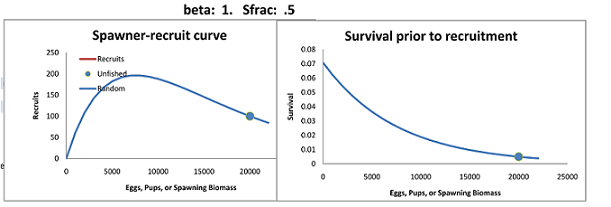
\includegraphics{survival_2}
	%\includegraphics{survival_3}
	%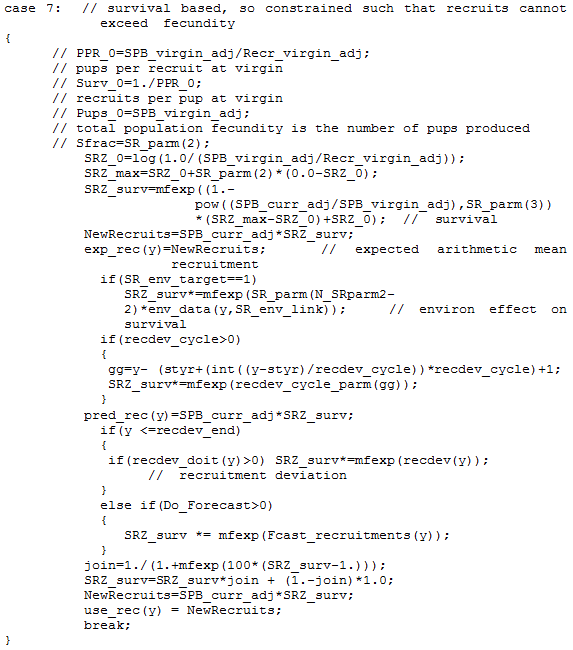
\includegraphics{survival_code}

	\item[Shepherd]\hfil\\
	\hypertarget{Shepard}{The} Shepherd stock recruit curve is calculated as:
	\begin{equation}
		R_y = \bigg(\frac{SB_y}{SB_0}\bigg)\frac{5hR_0SB^c_0(1-0.2^c)}{(1-h_{adj}0.2^c)+(5h_{adj}-1)SB^c_y}e^{-0.5b_y\sigma^2_R+\tilde{R}_y}\qquad \tilde{R}_y\sim N(0;\sigma^2_R)
	\end{equation}
	where c is the shape parameter for the stock recruitment curve, and $h_{adj}$ is the transformed steepness parameter defined as:
	\begin{equation}
		h_{adj}=\frac{\big(0.2+(h-0.2)\big)\big(1-0.2(5-0.2^c)\big)}{4*0.2^c}
	\end{equation}
\end{description}

\subsubsection{Recruitment Eras}
Conceptually, SS treats the early, data-poor period, the main data-rich period, and the recent/forecast time period as three eras along a continuum.  The user has control of the break year between eras.  Each era has its own vector.  The early era is defined as a vector (prior to V3.10 this was a dev\_vector) so it can have zeros during the earliest years not informed by data and then a few years with non-zero values without imposing a zero-centering on this collection of deviations.  The main era can be a vector of simple deviations, or a dev\_vector but it is normally implemented as a dev\_vector so that the spawner-recruitment function is its central tendency.  The last era does not force a zero-centered deviation vector so it can have zeros during the actual forecast and non-zero values in last few years of the time series.  The early and last eras are optional, but their use can help prevent SS from balancing a preponderance of negative deviations in early years against a preponderance of positive deviations in later years.  When the 3 eras are used, it would be typically to turn on the main era during an early model phase, turn on the early era during a later phase, then have the last era turn on in the final phase.

\subsubsection{Recruitment Likelihood}
In SS2, recruitment log(L) contained a term, + N\_forecast\_rec\_devs*log(sigmaR).  This meant that the total log(L) changed according to how many forecast years were included in the model scenario.  Worse, if sigmaR was allowed to be estimated by SS2, then this term would cause all the zero deviations during the forecast period to drag the overall estimated value of sigmaR down.  This problem is rectified in SS V3.  Now, for each year in the total time series (early, mid, late/forecast) the contribution of that year to the logL is equal to:  $dev^2/(2.0*sigmaR^2)+offset*log(sigmaR)$; where offset is the magnitude of the adjustment between the arithmetic and geometric mean of expected recruitment for that year.  With this approach, years with a zero or small offset value do not contribute to the second component.  With this approach, sigmaR may be estimable when there is good data to establish the time series of recruitment deviations.  In the likegfish example, turning on estimate of sigmaR results in an estimated value that is very close to the root mean squared error (rmse) of the estimated recruitment deviations.

\subsubsection{Recruitment Bias Adjustment}
The recruitment bias adjustment implemented in SS is based upon the work being documented in Methot and Taylor (2011) and following the work of Maunder and Deriso (2003).  The concept is based upon the following logic.  SigmaR represents the true variability of recruitment in the population.  It provides the constraining penalty for the estimates of recruitment deviations and it is not affected by data.  Where data that are informative about recruitment deviations are available, the total variability in recruitment, sigmaR, is partitioned into a signal (the variability among the recruitment estimates) and the residual, the variance of each recruitment estimate (see eq. below).  Where there are no data, no signal can be estimated and the individual recruitment deviations collapse towards 0.0 and the variance of each recruitment deviation approaches sigmaR.  Conversely, where there highly informative data about the recruitment deviations, then the variability among the estimated recruitment deviations will approach sigmaR and the variance of each recruitment deviation will approach zero.  Perfect data will estimate the recruitment time series signal perfectly.  Of course, we never have perfect data so we should always expect the estimated signal (variability among the recruitment deviations) to be less than the true population recruitment variability.
\begin{equation}
	SE(\hat{r}_y)^2 + SD(\hat{r})^2=\Bigg( \bigg( \frac{1}{\sigma^2_d}+\frac{1}{\sigma^2_R}\bigg)^{-1/2}\Bigg)^2+\Bigg( \frac{\sigma^2_R}{(\sigma^2_R+\sigma^2_d)^{1/2}}\Bigg)^2=\sigma^2_R
\end{equation}

The correct offset (bias adjustment) to apply to the expected value for recruitment is based on the concept that a time series of estimated recruitments should be mean unbiased, not median unbiased, because the biomass of a stock depends upon the cumulative number of recruits, which is dominated by the large recruitments.  The degree of offset depends upon the degree of recruitment signal that can be estimated.  Where no recruitment signal can be estimated, the median recruitment is the same as the mean recruitment, so no offset is applied.  Where lognormal recruitment signal can be estimated, the mean recruitment will be greater than the median recruitment.  The value

\begin{equation}
	b_y=\frac{E\Big( SD(\hat{r}_y)\Big)^2}{\sigma^2_R}=1-\frac{SE(\hat{r}_y)^2}{\sigma^2_R}
\end{equation}

\noindent of the offset then depends upon the partitioning of sigmaR into between and within recruitment variability.  The most appropriate degree of bias adjustment can be approximated from the relationship among sigmaR, recruitment variability (the signal), and recruitment residual error.

\begin{center}
	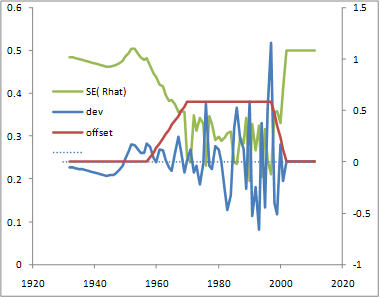
\includegraphics{10_bias}
\end{center}

Because the quantity and quality of data varies during a time series, SS allows the user to control the rate at which the offset is ramped in during the early, data-poor years, and then ramped back to zero for the forecast years.
On output to report.sso, SS calculates the mean bias adjustment during the early and main eras and compares it to the rmse of estimated recruitment devs.  A warning is generated if the rmse is small and the bias adjustment is larger than 2.0 times the ratio of $rmse^2$ to $sigmaR^2$.

In MCMC mode, the model still draws recruitment deviations from the lognormal distribution, so the full offset is used such that the expected mean recruitment from this lognormal distribution will stay equal to the mean from the spawner-recruitment curve. When SS reaches the MCMC and MCEVAL phases, all biasadj values are set to 1.0 for all active recruitment deviations because the model is now re-sampling from the full lognormal distribution of each recruitment.

\subsubsection{Recruitment Autocorrelation}
The autocorrelation parameter is implemented.  It is not performance tested and it has no effect on the calculation of the offsets described in the section above.

\subsubsection{Recruitment Cycle}
When SS is configured such that seasons are modeled as years, the concept of season within year disappears.  However, there may be reason to still want to model a repeating pattern in expected recruitment to track an actual seasonal cycle in recruitment.  If the recruitment cycle factor is set to a positive integer, this value is interpreted as the number of time units in the cycle and this number of full parameter lines will be read.  The cyclic effect is modeled as an exp(p) factor times R0, so a parameter value of 0.0 has nil effect.  In order to maintain the same number of total recruits over the duration of the cycle, a penalty is introduced so that the cumulative effect of the cycle produces the same number of recruits as Ncycles * R0.  Because the cyclic factor operates as an exponential, this penalty is different than a penalty that would cause the sum of the cyclic factors to be 0.0.  This is done by adding a penalty to the parameter likelihood, where:
\begin{equation}
	\begin{split}
				   X & = \sum(e^p)  \\
				   Y & = Ncycle  \\
				   Penalty & = 100000*(X-Y)^2
	\end{split}
\end{equation}

\subsubsection{Initial Age Composition}
A non-equilibrium initial age composition is achieved by setting the first year of the recruitment deviations before the model start year.  These pre-start year recruitment deviations will be applied to the initial equilibrium age composition to adjust this composition before starting the time series.  The model first applies the initial F level to an equilibrium age composition to get a preliminary N-at-age vector, then it applies the recruitment deviations for the specified number of younger ages in this vector.  If the number of estimated ages in the initial age composition is less than Nages, then the older ages will retain their equilibrium levels.  Because the older ages in the initial age composition will have progressively less information from which to estimate their true deviation, the start of the bias adjustment should be set accordingly.

\subsubsection{Fishing Mortality Method}
There are now three methods available for calculation of fishing mortality.  These are:  Pope’s approximation, continuous F with each F as a model parameter, and a hybrid method that does a Pope’s approximation to provide initial values for iterative adjustment of the continuous F values to closely approximate the observed catch.  With the hybrid method, the final values are in terms of continuous F, but do not need to be specified as full parameters.  In a 2 fishery, low F case, it is just as fast as the Pope approx. and produces identical result.  When F is very high, the problem becomes quite stiff for Pope’s and the hybrid method so convergence may slow.  It may still be better to use F option 2 (continuous F as full parameters) in these high F cases.  F as parameter is also preferred for situations where catch is known imprecisely and you are willing to accept a solution in which the final F values do not reproduce the input catch levels exactly.  Option 1 (Pope’s approx) still exists, but it is recommended to switch to option 3.

\begin{center}
		\begin{longtable}{p{1cm} p{3cm} p{11.3cm}}
			\multicolumn{3}{l}{Control file continued:}\\
			\hline
			Value &   &  Description\\
			\hline
			\endfirsthead

			\hline
			Value &  &  Description\\
			\hline
			\endhead

			%\hline
			\endfoot
			\endlastfoot

			0.2 & & F ballpark\\
			    & & This value is compared to the sum of the F’s for the specified year.  The sum is over all seasons and areas.  The lambda for the comparison goes down by a factor of 10 each phase and goes to 0.0 in the final phase.\\
		   \hline
			-1990 & & F ballpark year \\
			      & & Negative value disable F ballpark \\
		   \hline
			 3  & & F Method \\
			    & & 1 = Pope's \\
			    & & 2 = Continuous F as a parameter \\
			    & & 3 = Hybrid F (recommended)\\
		   \hline
		   2.9 & & Maximum F \\
		       & & This maximum is applied within each season and area.   A value of 0.9 is recommended for F method 1, and a value of about 4 is recommended for F method 2 and 3. \\
		   \hline
		   \multicolumn{3}{l}{COND: Depending on the F method} \\
		   \hline
		   \multicolumn{3}{l}{COND = 1: No additional input for Pope's approximation}\\
		   \hline
		   \multicolumn{3}{l}{COND = 2: Continuous F}\\
		   & 0.10 & Starting value for each F.  Initializing value for each F parameter.\\
		   & 1 & Phase for F parameters becoming active.  \\
		   &   & For phases prior to this value,  SS will use the hybrid option and the F values so calculated become the starting values for the F parameters when this phase is reached.\\
		   & 1 & Number of detailed F inputs to read below. \\
		   \hline
		   \multicolumn{3}{l}{COND = 3: Hybrid F}\\
		   & 4 & Number of tuning iterations in hybrid method. A value of 2 or 3 is sufficient with a single fleet and low Fs.  A value of 5 or so may be needed to match the catch near exactly when there are many fleets and high F. \\
		   \hline
		   \multicolumn{3}{l}{If F method = 2 and N for F detail is > 0}\\
		   & 1 1980 1 0.20 0.05 4 & fleet, year, season, F, SE, phase - these values override the catch se values in the data file and the overall starting F value and phase read just above.\\
		   \hline
	\end{longtable}
\end{center}

\subsubsection{Initial Fishing Mortality}
Read a short parameter setup line for each fishery.  The parameters are the fishing mortalities for the initial equilibrium.  Do not try to estimate parameters for fisheries with zero initial equilibrium catch.  If there is catch, then give a starting value greater than zero and it generally is best to estimate the parameter in phase 1.

It is possible to use the initial F method to achieve an estimate of the initial equilibrium Z in cases where the initial equilibrium catch is unknown.  To do this:
\begin{itemize}
	\item Include a positive value for the initial equilibrium catch;
	\item Set the lambda for the logL for initial equilibrium catch to a nil value (hence causing SS to ignore the lack of fit to the input catch level;
	\item Allow the initial F parameter to be estimated.  It will be influenced by the early age and size comps which should have some information about the early levels of Z.
\end{itemize}

\hypertarget{Qsetup}{}
\subsubsection{Catchability}
For each fishery and survey, enter a row with these 4 entries as described below:

\begin{enumerate}
	\item Fleet Number
	\item Link type: An assumed functional form between Q, the expected value, and the survey observation.
	\begin{enumerate}
		\item 1 = simple Q, proportional assumption about Q: $y=q*x$.
		%, establish a parameter to create environmental effect on Q, where the integer is the index of the environmental variable to be linked.  The relationship is:  $ ln(q_y) = ln(q_{base}) + Q_{env\_link\_para}*Env\_Value_y$.
		\item 2 = mirror simple Q, 1 mirrored parameter.  %Assumes proportional with offset: $y=q(x-a)$.
		\item 3 = Q with power, 2 parameters establish a parameter for non-linearity in survey-abundance linkage.  Assumes proportional with offset and power function: $y=q(x-a)^c$.
	\end{enumerate}
	\item Extra input for link (i.e. mirror fleet)
	\begin{enumerate}
		\item >0 = mirror the Q from another (lower numbered survey designated by abs(value))
	\end{enumerate}
	\item Do extra SD
	\begin{enumerate}
		\item 0 = skip (typical)
		\item 1 = estimate a parameter that will contain an additive constant to be added to the input stddev of the survey variability.  This extra SD approach is highly redundant with the older code that provided for iterative input of variance adjustment factors.  The newer code for extra SD estimation is recommended.
	\end{enumerate}
	\item Bias adjustment
	\begin{enumerate}
		\item 0 = no bias adjustment applied
		\item 1 = apply bias adjustment
	\end{enumerate}
	\item Q float
	\begin{enumerate}
		\item 0 = no float 
		\item 1 = float  %Makes Q as a mean unbiased float assignment.
	\end{enumerate}
	
	%\item Q Type
	%\begin{enumerate}
	%	\item <0 = mirror the Q from another (lower numbered survey designated by abs(value))
	%	\item 0 = set Q as a scaling factor such that the estimate is median unbiased.  This is comparable to the old “float” option.  This option is not available if a normal error structure is used.
	%	\item 2 = establish one parameter that will be the ln(Q).  Note that Q is in log units even if the error structure is normal.
	%	\item 3 = establish one parameter that will be the base ln(Q) and a set of additional parameters for each year of the survey that will be deviations in ln(Q).  These deviation parameters are full parameters, so each has a prior and variance, so surveys with high uncertainty in their calibration can be given a more diffuse prior to allow a larger deviation.  Because each of these Q deviations is coded as a separate parameter, rather than a member of a deviation vector, the contribution of these deviations to the model’s objective function is captured in the parameter prior section.  However, because there is no inherent constraint that these deviations have a zero sum, a separate log(L) contribution is calculated from the sum of the deviations ($(1+(\sum(devs))^2)^2-1$) and added to the “parm\_dev\_like” component.
	%	\item 4 = establish one parameter that will be the base ln(Q) and used as the Q for the first survey observation.  Subsequent N-1 parameters for remaining survey observations will be deviations in random walk of ln(Q).  These deviation parameters are otherwise treated identically to those generated by option (3) above, except that the extra contribution for the mean deviation is not calculated.
	%	\item 5 = This option will calculate the survey Q according to mean unbiased scaling, then assigns this value to the parameter (which must be set up in the control file and be given a negative phase).  Advantage is that the calculated Q can now have a prior.
	%\end{enumerate}
\end{enumerate}


\begin{center}
	\begin{longtable}{p{2cm} p{2cm} p{2cm} p{2cm} p{2cm} p{1.5cm} p{2.5cm}}
		\multicolumn{7}{l}{So for a setup with 2 fisheries and 2 surveys, the Q setup matrix could be:}\\
		\hline
	    \#Fleet Num. & Link Type & Link Info & Extra SD & Bias Adjust & Float  & Label \\
	    \hline
%	    1 & 1 & 0 & 1 & 0 & 0 & \#Fishery 1 \\
%	    2 & 1 & 0 & 1 & 0 & 0 & \#Fishery 2 \\
	    3 & 1 & 0 & 0 & 0 & 0 & \#Survey 1 \\
	    4 & 1 & 0 & 1 & 0 & 0 & \#Survey 2 \\
	    -9999 & 1 & 0 & 1 & 0 & 0 & \#End Read \\
	    \hline
	\end{longtable}
\end{center}

%Note: The deviation standard deviation line (in the 13 long parameter line section) does not do anything and is considered an used option.  The env-var column will replace this functionality

%\noindent Q types
%\begin{itemize}
%	\item <0 = mirror another fleet
%	\item 0 = float no bias adjustment
%	\item 1 = float bias adjustment
%	\item 2 = parameter no bias adjustment
%	\item 3 = parameter with random deviations
%	\item 4 = parameter with random walk
%	\item 5 = mean unbiased float assignment to parameter
%\end{itemize}

%\noindent COND: If any fishery or survey uses random devs or random walk, there is an option to either read detailed input to set up the deviation, or to just read a template.

%\begin{center}
%	\begin{longtable}{p{2.75cm} p{2.75cm} p{2.75cm} p{2cm} p{2cm} p{2cm}}
%		\endfirsthead

%		\hline
%		\#Value & Label & \multicolumn{4}{l}{Label, Description, and Options} \\
%		\hline
%		\endhead

%		\endfoot
%		\endlastfoot

%		\hline
%		\#Value & Label & \multicolumn{4}{l}{Label, Description, and Options} \\
%		\hline
%		1 & Random effects & \multicolumn{4}{l}{\multirow{2}{10cm}{0:  read one parameter line and use it as a template to create a time series of parameters for each observation for each fleet/survey that uses random effects.  The output to control.ss\_new will be in detailed format even if the input is not detailed.  Therefore a simple way to create a detailed setup file is to start with a simple template then edit the control.ss\_new file to create a detailed input for subsequent model runs;}}\\
%		\\
%		\\
%		\\
%		\\
%		\\
%		\\
%		\\
%		&  & \multicolumn{4}{l}{\multirow{2}{8cm}{1:  read a parameter line for each observation of each fleet/survey that uses random effects, thus allowing customization.  If the Q option for a fleet is 3 (random devs), then read one parameter for each observation.  If the Q option is 4, then read (N observations -1) parameters.}}\\
%		\\
%		\\
%		\\
%		\\
%		\\
%		\\
%		\hline
%	\end{longtable}
%\end{center}


%\noindent For each positive element in columns for the catchability (Q) setup above, read a long parameter setup line.  The order is: fishery 1 through survey N within power transformation, then within environment link, then within extra standard deviation, then within Q.  If no elements are selected, then there must be no parameter setup lines.

\begin{center}
	\begin{longtable}{p{1.1cm} p{1.1cm} p{1.2cm} p{1.2cm} p{1.5cm} p{1.1cm} p{1.5cm} p{4.3cm}}
		\endfirsthead

		\hline
		\#LO & HI & INIT & PRIOR & PR TYPE & SD & PHASE & LABEL \\
		\hline
		\endhead

		\hline
		\endfoot
		\endlastfoot

		\multicolumn{8}{l}{The list of parameters to be read from the above setup would be:}\\
		\hline
		\#LO & HI & INIT & PRIOR & PR TYPE & ... & BLOCK FXN & LABEL \\
		\hline
		%0  & 3   & 1    & 1    & 0  & ...  & 0   & \#Fishery1 power\\
		%0  & 0.5 & 0.10 & 0.10 & 0  & ...  & 0   & \#Fishery1 extra SD\\
		%0  & 0.5 & 0.10 & 0.10 & 0  & ...  & 0   & \#Fishery2 extra SD\\
		%0  & 0.5 & 0.10 & 0.10 & 0  & ...  & 0   & \#Survey2 extra SD\\
		%-7 & 5   & 0.50 & 0.50 & -1 & ...  & 0   & \#Fishery1 base Q\\
		%-7 & 5   & 0.50 & 0.50 & -1 & ...  & 0   & \#Fishery2 base Q\\
		-7 & 5   & 0.50 & 0.50 & -1 & ...  & 0   & \#Survey1 LnQ base\\
		-7 & 5   & 0.50 & 0.50 & -1 & ...  & 0   & \#Survey2 LnQ base\\
		%0  & 1   & 0    & 0    & 1  & ...  & 0   & \#Survey1 Q Random Walk obs2\\
		%0  & 1   & 0    & 0    & 1  & ...  & 0   & \#Survey1 Q Random Walk obs3\\
		%0  & 1   & 0    & 0    & 1  & ...  & 0   & \#Survey1 Q Random Walk obs4\\
		%... & ... & ... & ...  & ...& ...  & ... & ... \\
		 0  & 0.5 & 0.0 & 0.0 & 1 & ...  & 0   & \#Survey1 Q extra SD\\
		\hline
	\end{longtable}
\end{center}

\subsubsection{Selectivity and Discard}
For each fleet and survey, read a definition line for size selectivity and retention.  The four values read from each line are:

\begin{description}
	\item[Pattern]\hfill\\
	Valid length selectivity pattern code.

	\hypertarget{DomeRetention}{}
	\item[Discard]\hfill\\
	(0/1/2/3/4 or -index)  If value is 1, then program will read 4 retention parameters after reading the specified number of selectivity parameters and all discarded fish are assumed dead.  If the value is 2, then the program will read 4 retention parameters and 4 discard mortality parameters.  If the value is 3, then no additional parameters are read and all fish are assumed discarded and dead. If the value is 4, then the program will read 7 retention parameters (for dome-shaped retention) and 4 discard mortality parameters.  If the value is a negative number, then it will mirror the retention and discard mortality pattern of the lower numbered fleet.

	\item[Male]\hfill\\
	(0/1/2/3/4)  If value is 1, then program will read 4 additional parameters to define the male selectivity relative to the female selectivity.  Anytime the male selectivity is caused to be greater than 1.0; the entire male/female matrix of selectivity values is scaled by the max so that the realized max is 1.0.  Hopefully this does not cause gradient problems.  If the value is 2, then the main selectivity parameters define male selectivity and female selectivity is estimated as an offset from male selectivity.  This alternative is preferable if female selectivity is less than male selectivity.  The option 3 is only available if the selectivity pattern is 1, 20, or 24 and it causes the male selectivity parameters to be offset from the female parameters, rather than the male selectivity being an offset from the female selectivity.

	\item[Special]\hfill\\
	(0/value).  This value is used in different ways depending on the context.  If the selectivity type is to mirror another selectivity type, then put the index of that source fleet or survey here.  It must refer to a lower numbered fleet/survey.  If the selectivity type is 6 (linear segment), then put the number of segments here.  If the selectivity type is 7, then put a 1 here to keep selectivity constant above the mean average size for old fish of morph 1.
\end{description}

For each fleet and survey, read a definition line for age selectivity.  The 4 values to be read are the same as for the size-selectivity.  However, the retention value must be set to 0.

\begin{center}
	\begin{longtable}{p{2cm} p{2cm} p{2cm} p{2cm} p{6.5cm} }
		\hline
		\multicolumn{5}{l}{\#Example Setup for Size Selectivity Types}\\
		\#Pattern & Discard & Male & Special & Label \\
		\hline
		1  & 2 & 0 & 0 & \#Fishery1\\
		1  & 0 & 0 & 0 & \#Survey1\\
		0  & 0 & 0 & 0 & \#Survey2\\
		\hline
		\multicolumn{5}{l}{\#Age Selectivity Types}\\
		\#Pattern & Discard & Male & Special & Label \\
		\hline
		11  & 0 & 0 & 0 & \#Fishery1\\
		11  & 0 & 0 & 0 & \#Survey1\\
		11  & 0 & 0 & 0 & \#Survey2\\
		\hline
	\end{longtable}
\end{center}

\subsubsection{Reading the Selectivity and Retention Parameters}
Read the required number of parameter setup lines as specified by the definition lines above.  The complete order of the parameter setup lines is:
\begin{enumerate}
	\item Size selectivity for fishery 1
	\item Retention for fishery 1 (if discard specified)
	\item Discard Mortality for fishery 1 (if discard specified)
	\item Male offsets for size selectivity for fishery 1 (if offsets used)
	\item <repeat for additional fleets and surveys>
	\item Age selectivity for fishery 1
	\item Male offsets for age selectivity for fishery 1 (if offsets used)
	\item <repeat for additional fleets and surveys>.
\end{enumerate}

\begin{center}
	\begin{longtable}{p{1.1cm} p{1.1cm} p{1.2cm} p{1.2cm} p{1.5cm} p{1.1cm} p{1.5cm} p{4.3cm}}
		\endfirsthead
		
		\hline
		\#LO & HI & INIT & PRIOR & PR TYPE & SD & PHASE & LABEL \\
		\hline
		\endhead
		
		\hline
		\endfoot
		\endlastfoot
		
		\multicolumn{8}{l}{The list of parameters to be read from the above setup would be:}\\
		\hline
		\#LO & HI & INIT & PRIOR & PR TYPE & ... & BLOCK FXN & LABEL \\
		\hline
		19    & 80   & 53.5 & 50  & 1 & ...  & 0   & \#SizeSel p1 fishery 1\\
		0.01  & 60   & 18.9 & 15  & 1 & ...  & 0   & \#SizeSel p2 fishery 1 \\
		20    & 70   & 38.6 & 40  & 0 & ...  & 0   & \#Retain p1 fishery 1\\
		0.1   & 10   & 6.5  & 1   & 0 & ...  & 0   & \#Retain p2 fishery 1\\
		0.001 & 1    & 0.98 & 1   & 0 & ...  & 0   & \#Retain p3 fishery 1\\
		-10   & 10   & 1    & 0   & 0 & ...  & 0   & \#Retain p4 fishery 1\\
		0.1   & 1    & 0.6  & 0.6 & 0 & ...  & 0   & \#DiscMort p1 fishery 1\\
		-2    & 2    & 0    & 0   & 0 & ...  & 0   & \#DiscMort p2 fishery 1\\
		20    & 70   & 40   & 40  & 0 & ...  & 0   & \#DiscMort p3 fishery 1\\
		0.1   & 10   & 1    & 1   & 0 & ...  & 0   & \#DiscMort p4 fishery 1\\
		19    & 80   & 53.5 & 50  & 1 & ...  & 0   & \#SizeSel p1 survey 1\\
		0.01  & 60   & 18.9 & 15  & 1 & ...  & 0   & \#SizeSel p2 survey 1 \\
		0     & 40   & 0    & 5   & -1 & ...  & 0   & \#AgeSel p1 fishery 1\\
		0     & 40   & 40   & 5   & -1 & ...  & 0   & \#AgeSel p2 fishery 1\\
		0     & 40   & 0    & 5   & -1 & ...  & 0   & \#AgeSel p1 survey 1\\
		0     & 40   & 40   & 5   & -1 & ...  & 0   & \#AgeSel p2 survey 1\\
		0     & 40   & 0    & 5   & -1 & ...  & 0   & \#AgeSel p1 survey 2\\
		0     & 40   & 0    & 5   & -1 & ...  & 0   & \#AgeSel p2 survey 2\\
		\hline
	\end{longtable}
\end{center}

\subsubsection{Selectivity Patterns}
The currently defined selectivity patterns, and corresponding required number of parameters, are:

\begin{center}
	\begin{longtable}{p{2cm} p{3cm} p{10cm}}
		\endfirsthead

		\hline
		Pattern & N Parameters & Description \\
		\hline
		\endhead

		%\hline
		\endfoot
		\endlastfoot

		\hline
		\multicolumn{3}{c}{SIZE SELECTIVITY}\\
		  &   &  \\
		Pattern & N Parameters & Description \\
		\hline
		0 & 0 & Selectivity equals 1.0 for all sizes \\
		1 & 2 & Logistic \\
		2 & 8 & Discontinued: Double logistic with defined peak (uses IF joiners). Use pattern \#8 instead.\\
		3 & 6 & Discontinued \\
		4 & 0 & Discontinued: Set size selectivity equal to female fecundity. Use pattern \#30 instead.\\
		5 & 2 & Mirror another selectivity. The two parameters select bin range.\\
		6 & 2 + special value & Non-parametric \\
		7 & 8 & Discontinued: Double logistic with defined peak, uses smooth joiners; special = 1 causes constant selectivity above Linf for morph 1.  Use pattern \#8.\\
		8 & 8 & Double logistic, with defined peak, uses smooth joiners; special=1 causes constant selectivity above Linf for morph 1.  \\
		9 & 6 & Simple double logistic with no defined peak.\\
		15 & 0 & Mirror another selectivity (same as for age selectivity).\\
		22 & 4 & Double normal; similar to CASAL.\\
		23 & 6 & Same as the double normal pattern \#24 except the final selectivity is now directly interpreted as the terminal selectivity value.\\\
		24 & 6 & Double normal with defined initial and final selectivity level – Recommended option.  Test using SELEX-24.xls. \\
		25 & 3 & Exponential-logistic \\
		27 & 3+2*N nodes & Cubic spline\\
		\hline
		%\\
		%\multicolumn{3}{c}{SPECIAL SELECTIVITY}\\
		%Pattern & N Parameters & Description \\
		%\hline
		%30 & 0 & Sets expected survey abundance equal to spawning biomass (population fecundity). \\
		%31 & 0 & Sets expected survey abundance equal to exp(recruitment deviation).  This is useful if environmental data is used as an index of recruitment variability. \\
		%32 & 0 & Sets expected survey abundance equal to exp(recruitment deviation ) * SpawnBiomass.  So this is recruitment without density-dependence (for pre-recruit survey) because most ecological logic places the density-dependent stage during the juvenile period following the larval stage that is most sensitive to environmental perturbation.\\
		%33 & 0 & Sets expected survey abundance equal to age-0 recruitment.\\
		%34 & 0 & Spawning biomass depletion (B/B0).\\
		%\hline
	\end{longtable}
\end{center}

%\begin{description}
%	\item[Notes on Special Selectivity Options:]\hfil
%	\begin{itemize}
%		\item Do not input any size/age composition data for surveys using pattern 30-33.
%		\item The "catchability" coefficient for these selectivity patterns 30-33 have all the general properties of the catchability coefficient for real surveys, e.g. they can be time-varying, use power relationship, etc.
%	\end{itemize}
%\end{description}

\begin{center}
	\begin{longtable}{p{2cm} p{3cm} p{10cm}}

		\endfirsthead

		\hline
		Pattern & N Parameters & Description \\
		\hline
		\endhead

		%\hline
		\endfoot
		\endlastfoot

		\hline
		\multicolumn{3}{c}{AGE SELECTIVITY}\\
		   &   &  \\
		Pattern & N Parameters & Description \\
		\hline
		10 & 0 & Age selectivity = 1.0 for all ages beginning at age 1.  If it is desired that age-0 fish be selected, then use pattern \#11 and set minimum age to 1.0. \\
		11 & 2 & Pick min-max age\\
		12 & 2 & Logistic\\
		13 & 8 & Double logistic, IF joiners.  Use discouraged.  Use pattern \#18 instead.\\
		14 & nages+1 & Each age, value at age is $\frac{1}{1+exp(-x)}$ \\
		15 & 0 & Mirror another selectivity\\
		16 & 2 & Coleraine single Gaussian\\
		17 & nages + 1 & Each age as random walk from previous age.  For all ages in the population beginning with Amin = 1 for the fishery and 2 for the survey, there is a corresponding set of selectivity parameters for each fleet, $p_a$. \hyperlink{RandWalk}{Click here for more information.}\\
		18 & 8 & Double logistic, with defined peak, uses smooth joiners.  \\
		19 & 6 & Simple double logistic with no defined peak.\\
		20 & 6 & Double normal with defined initial and final level.  Recommended option. Test using SELEX-24.xls.\\
		26 & 3 & Exponential logistic\\
		27 & 3+2*N\_nodes & Cubic Spline\\
		\hline
	\end{longtable}
\end{center}

\subsubsection{Selectivity Pattern Details}
\begin{description}
	\item[Pattern \#1 (size) and \#12 (age) - Simple Logistic]\hfill\\
	Within SS logistic selectivity for the primary sex (if selectivity varies by sex) is formulated as:
	\begin{equation}
	S_l = \frac{1.0}{1+exp(-ln(19)(L_l - p1)/p2)}
	\end{equation}
	where $L_l$ is the length bin.  If age based selectivity is selected then the length bin is replaced by the age vector. If sex specific selectivity is specified the non-primary sex the p1 and p2 parameters are estimated as offsets.  Note that with a large p2 parameter, selectivity may not reach 1.0 at the largest size bin. The parameters are:
		\begin{itemize}
			\item p1 - size/age at inflection
			\item p2 - width for 95\% selection; a negative width causes a descending curve.
		\end{itemize}
\end{description}


\begin{description}
	\item[Pattern \#5 (size) - Mirror Selectivity]\hfil\\
	Two parameters select the min and max bin number (not min max size) of the source pattern.  If first parameter has value <=0, then interpreted as a value of 1 (e.g. first bin).  If second parameter has value <=0, then interpreted as nlength (e.g. last bin). The source pattern must have a lower type number
\end{description}	


\begin{description}
	\item[Pattern \#6 (size) - Non-parametric selectivity]\hfil\\
	Non-parametric size selectivity uses a set of linear segments.  The first waypoint is at Length = p1 and the last waypoint is at Length = p2.  The total number of waypoints is specified by the value of the Special factor in the selectivity set-up, so the N intervals is one less than the number of waypoints.  Intermediate waypoints are located at equidistant intervals between p1 and p2.  Parameters 3 to N are the selectivity values at the waypoints, entered as logistic, e.g. $1/(1+exp(-x))$.  Ramps from –10 to p3 if L<p1.  Constant at pN if L>p2.  Note that prior to version 3.03 the waypoints were specified in terms of bin number, rather than length.
\end{description}

\begin{description}
	\item[Pattern \#8 (size) and \#18 (age) - Double Logistic]\hfil
	\begin{itemize}
		\item  p1 – PEAK:  size (age) for peak. Should be an integer and should be at bin boundary and not estimated.  But options 7 and 18 may allow estimation.
		\item p2 – INIT:  selectivity at lengthbin=1 (minL) or age=0.
		\item p3 – INIT:  selectivity at lengthbin=1 (minL) or age=0. A logit transform $(1/(1+exp(-x))$ is used so that the transformed value will be between 0 and 1.  So a p1 value of –1.1 will be transformed to 0.25 and used to set the selectivity equal to 0.5 at a size (age) equal to 0.25 of the way between minL and PEAK. 
		\item p4 – SLOPE1:  log(slope) of left side (ascending) selectivity.
		\item p5 – FINAL:  logit transform for selectivity at maxL (or maxage).
		\item p6 – INFL2:  logit transform for size(age) at right side selectivity equal to half way between PEAK+PEAKWIDTH and maxL (or max age).
		\item p7 – SLOPE2:  log(slope) of right side (descending) selectivity
		\item p8 – PEAKWIDTH:  in width of flattop.
	\end{itemize}
\end{description}

\begin{description}
	\item[Pattern \#14 (age) - Revise Age]\hfil\\
	Age-selectivity pattern \#14 to allow selectivity-at-age to be the same as selectivity at the next younger age.  When using this option, the range on each parameter should be approximately -5 to 9 to prevent the parameters from drifting into extreme values with nil gradient. SS calculates the age-based selectivity as where $a = 1$ to $a = Amax + 1$:
	\begin{equation}
		 \begin{split}
		 temp = 9 - max(p(a))\\
		S_a = \frac{1}{1+exp(-(p(a+1) + temp))}
		\end{split}
	\end{equation}	
\end{description}

\begin{description}
	\item[Pattern \#17 (age) - Random Walk]\hfill\\
	This selectivity pattern provides for a random walk in ln(selectivity).  In typical usage:
	\begin{itemize}
		\item First parameter (for age 0) could have a value of -1000 so that the age 0 fish would get a selectivity of 0.0;
		\item 	Second parameter (for age 1) could have a value of 0.0 and not be estimated, so age 1 is the reference age against which subsequent changes occur;
		\item 	Next parameters get estimated values.  To assure that selectivity increases for the younger ages, the parameter min for these parameters could be set to 0.0 or a slightly negative value.
		\item If dome-shaped selectivity is expected, then the parameters for older ages could have a range with the max set to 0.0 so they cannot increase further.
		\item To keep selectivity at a particular age the same as selectivity at the next younger age, set its parameter value to 0.0 and not estimated.  This allows for all older ages to have the same selectivity.
		\item 	To keep a constant rate of change in selectivity across a range of ages, use the -999 flag to keep the same rate of change in ln(selectivity) as for the previous age.
		\item  Code for implementing random walk selectivity within SS can be found in Appendix C. \hyperlink{RandWalkSelex}{\textit{Click here for more information.}}
	\end{itemize}
\end{description}

\begin{description}
	\item[Pattern \#9 (size) and \#19 (age) - Simple Double Logistic with no defined peak]\hfil
	\begin{itemize}
		\item p1 - INFL1:  ascending inflection size (in cm)
		\item p2 – SLOPE1:  ascending slope
		\item p3 – INFL2:  descending inflection size (in cm)
		\item p4 – SLOPE2:  descending slope
		\item p5 – first BIN: bin number for the first bin with non-zero selectivity (must be an integer bin number, not a size)
		\item p6 – offset:  enter 0 if P3 is independent of P1; enter 1 if P3 is an offset from P1
	\end{itemize}
\end{description}

\begin{description}
	\item[Pattern \#22 (size) - Double Normal with Plateau]\hfil
	\begin{itemize}
		\item p1 – PEAK1:  beginning size for the plateau (in cm)
		\item p2 – PEAK2:  ending size for the plateau.  Calculated as a fraction of the distance between PEAK1 and 99\% of the lower edge of the last size bin in the model.  Transformed as (1/(1+exp(-p2)).   So a value of 0 results in PEAK2 being halfway between PEAK1 and 99\% of the last bin
		\item p3 – upslope:  ln(variance) on ascending side
		\item p4 – downslope:  ln(variance) on descending side
	\end{itemize}
\end{description}

\begin{description}
	\item[Pattern\#23 (size) and \#24 (size) - Double Normal Selectivity]\hfil
	\begin{itemize}
		\item p1 – PEAK:  beginning size for the plateau (in cm)
		\item p2 – TOP:  width of plateau, as logistic between PEAK and MAXLEN
		\item p3 – ASC-WIDTH:  parameter value is ln(width)
		\item p4 – DESC-WIDTH:  parameter value is ln(width)
		\item p5 – INIT:  selectivity at first bin, as logistic between 0 and 1.
		\item p6 – FINAL: selectivity at last bin, as logistic between 0 and 1.  (for pattern \#24) or
		\item p6 – FINAL: selectivity at last bin, as absolute value, so can be >1.0.  (for pattern \#23).  Warning:  Do not allow this value to go above 1.0 if the F\_method uses Pope’s approximation.  OK to go above 1.0 when F is in exponential form.  When this parameter is above 1.0, the overall selectivity pattern will have an intermediate plateau at 1.0 (according to peak and top), then will ascend further to the final value.
	\end{itemize}
	Notes for Double Normal Selectivity:
	\begin{itemize}
		\item See spreadsheet SELEX-24.xls for parameterization example.
		\item For the initial selectivity parameter (\#5)
		\begin{itemize}
			\item -999 or –1000:   ignore the initial selectivity algorithm and simply decay the small fish selectivity according to P3,
			\item < -1000:  ignore the initial selectivity algorithm as above and then set selectivity equal to 1.0e-06 for size bins 1 through bin =  -1001 –value.  So a value of –1003 would set selectivity to a nil level for bins 1 through 2 and begin using the modeled selectivity in bin 3.
		\end{itemize}
		\item For the final selectivity parameter (\#6)
		\begin{itemize}
			\item -999 or –1000:   ignore the final selectivity algorithm and simply decay the large fish selectivity according to parameter \#4,
			\item <-1000:  set selectivity constant for bins greater than bin number =  -1000 – value.
		\end{itemize}
	\end{itemize}
	Selectivity pattern \#24, double normal, showing sub-functions and steep logistic joiners:
	\begin{center}
		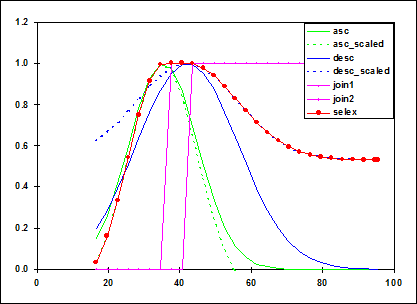
\includegraphics{DoubleNormal}
	\end{center}
\end{description}

\begin{description}
	\item[Pattern \#15 (age) - Mirror]\hfil\\
	No parameters.  Whole age range is mirrored from a user-specified fleet.
\end{description}

\begin{description}
	\item[Pattern \#16 - Gaussian (similar to Coleraine)]\hfil
	\begin{itemize}
		\item p1 – age below which selectivity declines
		\item p2 – scaling factor for decline
	\end{itemize}
\end{description}

\begin{description}
	\item[Pattern \#9 (size) and \#19 (age) - Simple Double Logistic]\hfil
	\begin{itemize}
		\item p1 – ascending inflection age/size
		\item p2 – ascending slope
		\item p3 – descending inflection age/size
		\item p4 – descending slope
		\item p5 – age or size at first selection; this is a specification parameter, so must not be estimated.  Enter integer that is age for pattern 19 and is bin number for pattern 9
		\item p6 – (0/1)  where a value of 0 causes the descending inflection to be a standalone parameter, and a value of 1 causes the descending inflection to be interpreted as an offset from the ascending inflection.  This is a specification parameter, so must not be estimated.
	\end{itemize}
	A value of 1.0e-6 is added to the selectivity for all ages, even those below the minage.\\
\end{description}

\begin{description}
	\item[Pattern \#25 (size) and \#26 (age) - Exponential logistic]\hfil
	\begin{itemize}
		\item p1 – ascending rate, min: 0.02, max: 1.0, reasonable start value:  0.1
		\item p2 – peak, as fraction of way between min size and max size.  Parameter min value:  0.01; max:  0.99; reasonable start value:  0.5
		\item p2 – minsize + p2*(maxsize-minsize)
		\item p3 – descending rate, min: 0.001, max: 0.5, reasonable start value:  0.01.  A value of 0.001 provides a nearly asymptotic curve.  Values above 0.2 provide strongly dome-shaped function in which the p3 and p1 parameters interact strongly.
	\end{itemize}
	\begin{equation}
	\frac{e^{p3*p1(p2'-size)}}{1-p3(1-e^{p1(p2'-size)})}
	\end{equation}
	Example: Exponential logistic selectivity with p1 = 0.30, p2 = 0.50, and p3 = 0.02:\\
	\begin{center}
		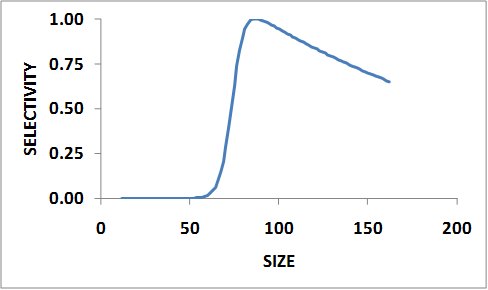
\includegraphics{ExpLogistic}
	\end{center}
\end{description}

\begin{description}
	\item[Pattern \#27 (size and age)- Cubic Spline]\hfil\\
	This selectivity pattern uses the ADMB implementation of the cubic spline function. This function requires input of the number of nodes, the positions of those nodes, the parameter values at those nodes, and the slope of the function at the first and last node.  In SS, the number of nodes is specified in the “special” column of the selectivity set-up.  The pattern number 27 is used to invoke cubic spline for size selectivity and for age selectivity; the input syntax is identical.\\
	\\
	For a 3 node setup, the SS input parameters would be:
	\begin{itemize}
		\item p1 – 	code for initial set-up (0, 1 or 2) as explained below
		\item p2 – 	gradient at the first node (should be a small positive value)
		\item p3 – 	gradient at the last node (should be zero or a small negative value)
		\item p4-p6 – the nodes in units of cm; must be in rank order and inside of the range of the population length bins.  These must be held constant (not estimated, e.g. negative phase value) during a model run.
		\item  p7-p9 – the values at the nodes.  Units are ln(selectivity).
	\end{itemize}
	Notes:
	\begin{itemize}
		\item There must be at least 3 nodes.
		\item One of these selectivity parameter values should be held constant so others are estimated relative to it.
		\item Selectivity is forced to be constant for sizes greater than the size at the last node
		\item The overall selectivity curve is scaled to have a peak equal to 1.0.
		\item Terminal nodes cannot be at the min or max population length bins.
	\end{itemize}
	
	Code for implementing cubic spline selectivity within SS can be found in Appendix C. \hyperlink{CubicSpline}{\textit{Click here for more information.}}\\

	
	The figure below compares a 3 node and a 6 node cubic spline with a 2 parameter logistic function.  In fitting these functions, the 2 cubic spline approaches fit slightly better than the logistic, presumably because the data were slightly indicative of a small dome in selectivity.\\
	\begin{center}
		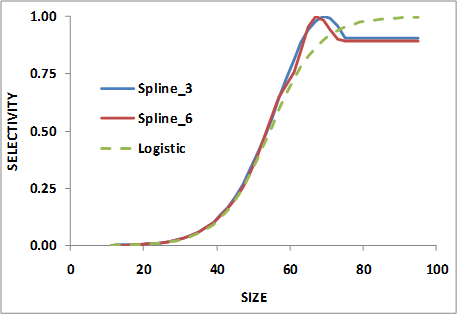
\includegraphics{CubicSpline}
	\end{center}
	
	Auto-Generation of Cubic Spline Control File Set-Up:\\
	A New SS feature pioneered with the cubic spline function is a capability to produce more specific parameter labels and to auto-generate selectivity parameter setup.  The auto-generation feature is controlled by the first selectivity parameter value for each fleet that is specified to use the cubic spline.  There are 3 possible values for this setup parameter:
	\begin{itemize}
		\item 0: no auto-generation, process parameter setup as read.
		\item 1: auto-generate the node locations based on the specified number of nodes and on the cumulative size distribution of the data for this fleet/survey.
		\item 2: auto-generate the nodes and also the min, max, prior, init, and phase for each parameter.
	\end{itemize}
	
	With either the auto-generate option \#1 or \#2, it still is necessary to include in the parameter file placeholder rows of values so that the init\_matrix command can input the current number of values because all selectivity parameter lines are read as a single matrix dimensioned as N parameters x 14 columns.  The read values of min, max, init, prior, prior type, prior stddev, and phase will be overwritten.
	
	Cumulative size and age distribution is calculated for each fleet, summing across all samples and both sexes.  These distributions are output in echoinput.sso and in a new OVERALL\_COMPS section of report.sso.
	
	When the nodes are auto-generated, the first node is placed at the size corresponding to the 2.5\% percentile of the cumulative size distribution, the last is placed at the 97.5\% percentile of the size distribution, and the remainder are placed at equally spaced percentiles along the cumulative size distribution.  These calculated node values are output into control.ss\_new.  So, the user could extract these nodes from control.ss\_new, edit them to desired values, then, insert them into the input control file.  Remember to turn off auto-generation in the revised control file.
	
	When the complete auto-generation is selected, the control.ss\_new would look like the table below:
	
	\begin{center}
		\begin{longtable}{p{1cm} p{1cm} p{1cm} p{1cm} p{1.75cm} p{1cm} p{1.2cm} p{1cm} p{3.8cm}}
			\#LO & HI & INIT & PR & PR\_TYPE & SD & PHASE &  ... & \#Label \\
			\hline
			0 &     2 &   2.0 & 0 & -1 & 0     & -99 & 0 & \#SizeSpline Code\\
			-0.001 & 	 1 &  0.13 & 0 &  1 & 0.001 & 	3 & 0 & \#SizeSpline GradLo\\
			-1 & 0.001 & -0.03 & 0 &  0 & 0.001 & 	3 & 0 & \#SizeSpline GradHi\\
			11 & 	95 & 	38 & 0 & -1 & 	  0 & -99 & 0 & \#SizeSpline Knot1\\
			11 & 	95 & 	59 & 0 & -1 &     0 & -99 & 0 & \#SizeSpline Knot2\\
			11 & 	95 & 	74 & 0 & -1 & 	  0 & -99 & 0 & \#SizeSpline Knot3\\
			-9 & 	 7 & 	-3 & 0 &  1 & 0.001 & 	2 & 0 & \#SizeSpline Value1\\
			-9 &   	 7 & 	-1 & 0 & -1 & 0.001 &  99 & 0 & \#SizeSpline Value2\\
			-9 & 	 7 & -0.78 & 0 &  1 & 0.001 & 	2 & 0 & \#SizeSpline Value3\\
			\hline
		\end{longtable}
	\end{center}
\end{description}

%\begin{description}
%	\item[Survey Pattern \#34 - Depletion]\hfil\\
%	This option allows a specified degree of stock depletion (in terms of spawning biomass) to be entered as the ratio of current year’s spawning biomass relative to Bzero.  With this option, it is not necessary or reasonable to estimate the Q for this fleet, but you must set ln(Q) = 0.0 as a fixed value for absolute abundance.  Also, if this option is used, then automatic adjustments to phase and lambda are made such that:
%	\begin{itemize}
%		\item all parameter phases are adjusted by +1 so that only R0 is active in phase 1
%		\item all lambdas are set to 0 in phase 1, except the lambda for this depletion survey.  Internally, the flag "depletion\_fleet" is turned on (= to the index of that fleet) if there is a fleet with selex = \#34
%	\end{itemize}
	
%	Essentially, these automated features cause SS to mimic DB-SRA in phase 1.  If the model is only run through phase 1, then this will be the final result.  Alternatively, use of this option could just be used to get the R0 parameter into a reasonable range before proceeding to estimate other parameters.  The lambda for the depletion survey could remain at 1.0 for the entire model run, or it could be reduced in later phases to prevent influencing final model results.
%\end{description}

\subsubsection{Retention}
Retention is defined as a logistic function of size.  It does not apply to surveys.  Four parameters (for asymptotic retention) or seven parameters (for dome-shaped retention) are used:
\begin{itemize}
	\item p1 – ascending inflection
	\item p2 – ascending slope
	\item p3 – maximum retention (often a time-varying quantity to match the observed amount of discard)
	\item p4 – male offset to ascending inflection (arithmetic, not multiplicative)
	\item p5 – descending inflection
	\item p6 – descending slope
	\item p7 – male offset to descending inflection (arithmetic, not multiplicative)
\end{itemize}
\begin{equation}
	\text{Retention} = \left(\frac{P3}{1 + e^{\frac{-(L-(P1+P4*male))}{P2}}}\right)*\left(1 - \frac{1}{1 + e^{\frac{-(L-(P5+P7*male))}{P6}}}\right)
\end{equation}

\subsubsection{Discard Mortality}
Discard mortality is defined as a logistic function of size such that mortality declines from 1.0 to an asymptotic level as fish get larger.  It does not apply to surveys and it does not affect the calculation of expected values for discard data.   It is applied so that the total mortality rate is:\\
\begin{center}
	deadfish = selex * (retain + (1.0-retain)*discmort)
\end{center}
If discmort is 1.0, all selected fish are dead; if discmort is 0.0, only the retained fish are dead.

Four parameters are used:
\begin{itemize}
	\item p1 – descending inflection
	\item p2 – descending slope
	\item p3 – maximum discard mortality
	\item p4 – male offset to descending inflection (arithmetic, not multiplicative)
\end{itemize}

Discard mortality is calculated as:
\begin{equation}
	\text{Mortality} = \left(1 - \frac{1-P3}{1+e^{\frac{-(L-(P1+P4*male))}{P2}}}\right)
\end{equation}

\subsubsection{Male Selectivity}
There are two approaches to specifying sex specific selectivity.  One approach allows male selectivity to be specified as a fraction of female selectivity (or vice versa).  This first approach can be used for any selectivity pattern.  The other option allows for separate selectivity parameters for each sex plus an additional parameter to define the scaling of one sex’s peak selectivity relative to the other sex’s peak.  This second approach has only been implemented for a few selectivity patterns.\\
\\
Approach \#1:\\
If the “domale” flag is set to 1, then the selectivity parameters define female selectivity and the offset defined below sets male selectivity relative to female selectivity.  The two sexes switch roles if the “domale” flag is set to 2.  Generally it is best to select the option so that the dependent sex has lower selectivity, thus obviating the need to rescale for selectivities that are greater than 1.0.  Sex specific selectivity is done the same way for all size and age selectivity options.
\begin{itemize}
	\item P1 – size (age) at which a dogleg occurs (set to an integer at a bin boundary and do not estimate)
	\item P2 – log(relative selectivity) at minL or age=0.  Typically this will be set to a value of 0.0 (for no offset) and not estimated.  It would be a rare circumstance in which the youngest/smallest fish had sex-specific selectivity.
	\item P3 – log(relative selectivity) at the dogleg
	\item P4 – log(relative selectivity) at maxL or max age.
\end{itemize}

For intermediate ages, the log values are linearly interpolated on size (age).

If selectivity for the dependent sex is greater than the selectivity for the first sex (which always peaks at 1.0), then the male-female selectivity matrix is rescaled to have a maximum of 1.0.\\
\\
Approach \#2:\\
A new sex selectivity option (3 or 4) has been implemented for size selectivity patterns 1 (logistic) and 23 and 24 (double normal) or age selectivity pattern 20 (double normal age).  Rather than calculate male selectivity as an offset from female selectivity, here the male selectivity is calculated by making the male parameters an offset from the female parameters (option 3), or females are offset from males with option 4.  The description below applies to option 3. If the size selectivity pattern is 1 (logistic), then read 3 parameters:
\begin{itemize}
	\item male parm 1 is added to the first selectivity parm (inflection)
	\item male parm 2 is added to the second selectivity parm (width of curve)
	\item male parm 3 is the asymptotic selectivity
\end{itemize}

If the size selectivity pattern is 20, 23 or 24 (double normal), then:
\begin{itemize}
	\item male parm 1 is added to the first selectivity parm (peak)
	\item male parm 2 is added to the third selectivity parm (width of ascending side); then exp(this sum) per previous transform
	\item male parm 3 is added to the fourth selectivity parm (width of descending side); then exp(sum) per previous transform
	\item male parm 4 is added to the sixth selectivity parm (selectivity at final size bin); then 1/(1+exp(-sum)) per previous transform
	\item male parm 5 is the apical selectivity for males
\end{itemize}

Note that the male selectivity offsets currently cannot be time-varying (need to check on this).  Because they are offsets from female selectivity, they inherit the time-varying characteristics of the female selectivity.


\subsubsection{Time-varying Options}
The time-varying options for selectivity parameters are identical to the time-varying options for biology parameters.  These options are described below in the Time-Varying Parameter Options section.  After reading the selectivity parameters, which will include possible instructions to create environmental link, blocks, or dev vectors, then read the following section.  Note that all inputs in this section are conditional (COND) on entries in the selectivity parameter section.  So if no selectivity parameters invoke any time-varying properties, this section is left blank (or completely commented out with \#).

\begin{center}
	\begin{longtable}{p{2cm} p{1cm} p{4cm} p{8cm}}
		Value & & Label & Description\\
		\hline
		\endfirsthead

		Value & & Label & Description\\
		\hline
		\endhead

		\endfoot

		\endlastfoot

			%Value & & Label & Description \\
			COND &  & & If any selectivity parameters use environmental linkage, then read next line and associated parameter line(s).\\
			     & 0 & Custom Environmental Linkage	& \\
			\hline
			COND &  & & If custom=0, then read one parameter line below and apply to all env functions;
			If custom>0, then read a setup line for each SEL-parm with Env-var>0. Note that control.ss\_new will write out with custom=1 so it can write all the parameter values.\\
			\hline
			\multicolumn{4}{l}{Enter proper number of short set-up lines (0, 1, several) for the SEL-parm environmental}\\
			\multicolumn{4}{l}{linkages.  Each line will have 7 values:  LO, HI, INIT, PRIOR, PR\_TYPE, SD, PHASE.}\\
			\hline
			COND & & & If any selectivity parameters use time blocks, then read next line and associated parameter line(s). \\
			     & 0 & Custom block setup & If custom=0, then read one setup and apply to all Block fxns;
			     If custom>0, then read a setup line for each SEL-parm with Block>0.  \\
			\hline
			\multicolumn{4}{l}{Enter proper number of short set-up lines (0, 1, several) for the SEL-parm block linkages.}\\
			\multicolumn{4}{l}{Each line will have 7 values:  LO, HI, INIT, PRIOR, PR\_TYPE, SD, PHASE.} \\
			\hline
			COND &  & & If any selectivity parameters use annual devs, then read  value\\
			     & -4 & Selparm dev phase & Phase in which selparm devs, if any, are estimated. \\
			\hline
			%COND &  & & If any selectivity parameters use environmental links, blocks or annual devs, then read value.\\
			%     & 2 & Selparm Adjust Method & 1 = parameter adjustments for env, block and dev are applied directly and resulting value is not compared to base parameter bounds\\
			%     &   & & 2 = parameter adjustments use a logistic transformation to assure that adjusted parameter value stays within bounds of base parameter.\\
			     %&  & & 3 = parameter adjustments use an additive random walk.\\
			     %&  & & 4 = parameter adjustments use a mean reverting random walk.\\
			%\hline
	\end{longtable}
\end{center}

For additional information on the use of time-varying parameters please see the \hyperlink{TVpara}{\textit{Using Time Varying Parameters}} section.

\subsubsection{Tag Recapture Parameters}
Specify if tagging data are being used:
\begin{center}
	\begin{longtable}{p{0.75cm} p{0.75cm} p{0.75cm} p{1.25cm} p{1.75cm} p{1cm} p{1.5cm} p{0.75cm} p{4.5cm}}

		\multicolumn{3}{l}{Value} &  \multicolumn{3}{l}{Label} & \multicolumn{3}{l}{Description}\\
		\hline
		\multicolumn{3}{l}{1} &  \multicolumn{3}{l}{Tagging Data Present} & \multicolumn{3}{l} {0 = no read}\\
		\multicolumn{3}{l}{} &  \multicolumn{3}{l}{} & \multicolumn{3}{l} {1 = read following lines}\\
		\\
		\multicolumn{8}{l}{COND = 1 Read the following long parameter lines:}\\
		\hline
		\#LO & HI & INIT & PRIOR & PR\_TYPE& SD & PHASE & ... & LABEL\\
		\hline
		-10 & 10 & 9 & 9 & 1 & 0.001 & -4 & 0 & \#TG loss init 1\\
		-10 & 10 & 9 & 9 & 1 & 0.001 & -4 & 0 & \#TG loss init 2\\
		-10 & 10 & 9 & 9 & 1 & 0.001 & -4 & 0 & \#TG loss init 3\\
		-10 & 10 & 9 & 9 & 1 & 0.001 & -4 & 0 & \#TG loss chronic1\\
		-10 & 10 & 9 & 9 & 1 & 0.001 & -4 & 0 & \#TG loss chronic2\\
		-10 & 10 & 9 & 9 & 1 & 0.001 & -4 & 0 & \#TG loss chronic3\\
		  1 & 10 & 2 & 2 & 1 & 0.001 & -4 & 0 & \#TG loss overdisperion1\\
		  1 & 10 & 2 & 2 & 1 & 0.001 & -4 & 0 & \#TG loss overdisperion2\\
		  1 & 10 & 2 & 2 & 1 & 0.001 & -4 & 0 & \#TG loss overdisperion3\\
		-10 & 10 & 9 & 9 & 1 & 0.001 & -4 & 0 & \#TG report fleet1\\
		-10 & 10 & 9 & 9 & 1 & 0.001 & -4 & 0 & \#TG report fleet2\\
		 -4 &  0 & 0 & 0 & 0 &     2 & -4 & 0 & \#TG report decay1\\
		 -4 &  0 & 0 & 0 & 0 &     2 & -4 & 0 & \#TG report decay2\\
		 \hline
	\end{longtable}
\end{center}

The tagging reporting rate parameter is transformed within SS during estimation to maintain a positive value and is reported according to the transformation:
\begin{equation}
	\text{Tagging Reporting Rate} = \frac{e^{\text{input parameter}}}{1+e^{\text{input parameter}}}
\end{equation}

\hypertarget{GcompVar}{}
\subsubsection{Variance Adjustment Factors}
When doing iterative reweighting of the input variance factors, it is convenient to do this in the control file, rather than the data file.  This section creates that capability.
\begin{center}
	\begin{longtable}{p{3cm} p{3cm} p{9.5cm} }

		%Value & Description & & Options & \\
		%\hline
		%0 & \multicolumn{2}{l}{Variance Adjustment Factors } & \multicolumn{2}{l}{0 = none, 1 = read table}\\
		 \multicolumn{3}{l}{Variance Adjustment Factors }\\
		 \hline
		-9999 1 0 & \multicolumn{2}{l}{No variance adjustment factors applied }\\
		\\
		\multicolumn{3}{l}{If variance adjustment factors are to be applied:}\\
		\hline
		%Fleet/Survey 1 & Fleet/Survey 2 & Fleet/Survey 3 & Fleet/Survey 4 & Label \\
		Factor & Fleet & Value \\
		\hline
		1 & 2 & 0.5 \\
		4 & 1 & 0.25 \\
		4 & 2 & 0.75 \\
		-9999 & 0 & 0 \\
		%0 & 0 & 0 & 0 & \#Survey CV\\
		%0 & 0 & 0 & 0 & \#Discard CV\\
		%0 & 0 & 0 & 0 & \#Mean BodyWght SD\\
		%1 & 1 & 1 & 1 & \#Length Comp\\
		%1 & 1 & 1 & 1 & \#Age Comp\\
		%1 & 1 & 1 & 1 & \#Size-at-Age\\
		%1 & 1 & 1 & 1 & \#Generalized Size Comp\\
		\hline
	\end{longtable}
\end{center}

\begin{description}
	\item[Additive Survey CV - Factor 1]\hfil\\
	The survey input variance (labeled survey CV) is actually the standard deviation of the ln(survey).  The variance adjustment is added directly to this standard deviation.  Set to 0.0 for no effect.  Negative values are OK, but will crash if adjusted value becomes negative.
	\item[Additive Discard - Factor 2]\hfil\\
	The input variance is the CV of the observation.  Because this will cause observations of near zero discard to appear overly precise, the variance adjustment is added to the discard standard deviation, not to the CV.  Set to 0.0 for no effect.
	\item[Additive Mean Body Weight - Factor 3]\hfil\\
	The input variance is in terms of the CV of the observation.  Because such data are typically not very noisy, the variance adjustment is added to the CV and then multiplied by the observation to get the adjusted standard deviation of the observation.
	\item[Multiplicative Length Composition - Factor 4]\hfil\\
	The input variance is in terms of an effective sample size.  The variance adjustment is multiplied times this sample size.  Set variance adjustment to 1.0 for no effect.
	\item[Multiplicative Age Composition - Factor 5]\hfill\\
	Age composition is treated the same way as length composition.
	\item[Multiplicative Size-at-Age - Factor 6]\hfill\\
	Size-at-age input variance is the sample size for the N observations at each age.  The variance adjustment is multiplied by these N values. Set to 1.0 for no effect.
	\item[Multiplicative Generalized Size Composition - Factor 7]\hfill\\
	Generalized size composition input variance is the sample size for each observation.  The variance adjustment for each fleet is multiplied by these sample sizes. Set to 1.0 for no effect.
	\item[Usage Notes]\hfill
	\begin{itemize}
		\item The report.sso output file contains information useful for determining if an adjustment of these input values is warranted to better match the scale of the average residual to the input variance scale.
		\item Because the actual input variance factors are modified, it is these modified variance factors that are used when creating parametric bootstrap data files.  So, the control files used to analyze bootstrap generated data files should have the variance adjustment factors reset to null levels.
	\end{itemize}
\end{description}

\subsubsection{Lambdas (Emphasis Factors)}
These values are multiplied by the corresponding likelihood component to calculate the overall negative log likelihood to be minimized.

\begin{center}
	\begin{tabular}{p{2cm} p{14cm}}
		Value & Description \\
		\hline
		4 & Max lambda phase: read this number of lambda values for each element below.  The last lambda value is used for all higher numbered phases.\\
		1 & sd offset; value=0 causes log(like) to omit the +log(s) term; value=1 causes log(like) to include the log(s) term for CPUE, discard, meanbodywt, recruitment deviations. \\
		\hline
	\end{tabular}
\end{center}

\begin{description}
	\item[Usage Note:]\hfil\\
	If the CV for size-at-age is being estimated and the model contains mean size-at-age data, then the flag for inclusion of the +log(stddev) term in the likelihood must be included.  Otherwise, the model will always get a better fit to the mean size-at-age data by increasing the parameter for CV of size-at-age.
\end{description}

The reading of the lambda values has been substantially altered with SS v3.  Instead of reading a matrix containing all the needed lambda values, SS now just reads those elements that will be given a value other than 1.0.  After reading the datafile, SS sets lambda equal to 0.0 if there are no data for a particular fleet/data type, and a value of 1.0 if data exist.  So beware if your data files had data but you had set the lambda to 0.0 in a previous version of SS.  First read an integer for the number of changes.

\begin{center}
	\begin{longtable}{p{3cm} p{3cm} p{2cm} p{3cm} p{3cm}}
		\hline
		%3 & \multicolumn{4}{l}{\#Number of changes to make to default lambdas (default value is 1.0)}\\
		\multicolumn{5}{l}{\#Then read that number of lines containing the change information:}\\
		\#Component & Fleet/Survey & Phase & Lambda & SizeFreq Method \\
		\hline
		1 & 2 & 2 & 1.5 & 1 \\
		4 & 2 & 2 & 10 & 1 \\
		4 & 2 & 3 & 0.2 & 1 \\
		-9999 & 1 & 1 & 1 & 1 \\
		\hline
	\end{longtable}
\end{center}


\begin{center}
	\begin{longtable}{p{1cm} p{6cm} p{1cm} p{6cm} }
		\multicolumn{4}{l}{The codes for component are:}\\
		\hline
		1 & survey & 10 & recruitment deviations \\	
		2 & discard & 11 & parameter priors\\		
		3 &  mean weight & 12 & parameter deviations\\	
		4 & length & 13 & crash penalty\\		
		5 & age & 14 & morph composition\\
		6 & size frequency & 15 & tag composition\\		
		7 & size-at-age & 16 & tag negative binomial\\
		8 & catch & 17 & F ballpark\\		
		9 & initial equilibrium catch & & \\
		\hline
	\end{longtable}
\end{center}


%\begin{center}
%	\begin{longtable}{p{2cm} p{2cm} p{2cm} p{2cm} p{6cm}}
		%\hline
%		\endfirsthead

%		\hline
%		\endhead
%		\hline
%
%		\endfoot
%		\endlastfoot
%
%		\multicolumn{5}{l}{On output to control.ss\_new, the full table is written:}\\
%		\multicolumn{5}{l}{\#Lambdas (for information only; columns are phases)}\\
%		\hline
%		\# 0 & 0 & 0 & 0 & \#CPUE/survey: 1\\
%		\# 1 & 1.5 & 1.5 & 1.5 & \#CPUE/survey: 2\\
%		\# 1 & 1 & 1 & 1 & \#CPUE/survey: 3\\
%		\# 1 & 1 & 1 & 1 & \#lencomp: 1\\
%		\# 1 & 10 & 2 & 2 & \#lencomp: 2\\
%		\# 0 & 0 & 0 & 0 & \#lencomp: 3\\
%		\# 1 & 1 & 1 & 1 & \#agecomp: 1\\
%		\# 1 & 1 & 1 & 1 & \#agecomp: 2\\
%		\# 0 & 0 & 0 & 0 & \#agecomp: 3\\
%		\# 1 & 1 & 1 & 1 & \#size-at-at-age: 1\\
%		\# 1 & 1 & 1 & 1 & \#size-at-at-age: 2\\
%		\# 0 & 0 & 0 & 0 & \#size-at-at-age: 3\\
%		\# 1 & 1 & 1 & 1 & \#init\_equil\_catch \\
%		\# 1 & 1 & 1 & 1 & \#recruitments \\
%		\# 1 & 1 & 1 & 1 & \#parameter priors\\
%		\# 1 & 1 & 1 & 1 & \#parameter dev vectors\\
%		\hline
%	\end{longtable}
%\end{center}

\subsubsection{Controls for Variance of Derived Quantities}
Additional standard deviation reported may be selected.
\begin{center}
	\begin{longtable}{p{1cm} p{1.2cm} p{1.2cm} p{1.2cm} p{1.2cm} p{1.2cm} p{1.5cm} p{1.5cm} p{1.8cm}}
		\hline
		1 & \multicolumn{8}{l}{0 = no additional std dev reporting, 1 = read values}\\
		\multicolumn{2}{l}{COND > 0} & \multicolumn{7}{l}{If the above value is "0", then do not include any more entries.}\\
		  & & \multicolumn{7}{l}{If the above value is "1", then read the 4 following lines:}\\
		Selex Type & Len/Age & Year & Nselex Bins & Growth Pattern & Ngrowth ages & Area for Natage & NatAge year  & N ages to report\\
		\hline
		1 & 1 & -1 & 5 & 1 & 5 & 1 & -1 & 5\\ 
		\hline
		\multicolumn{9}{l}{\#Vector with selex std bin picks (-1 in first bin to self-generate).} \\
		5 & 15 & 25 & 35 & 43 & & & & \\
		\hline
		\multicolumn{9}{l}{\#Vector with growth std bin picks (-1 in first bin to self-generate).} \\	
		1 & 2 & 14 & 26 & 40 & & & & \\	
		\hline
		\multicolumn{9}{l}{\#Vector with NatAge std bin picks (-1 in first bin to self-generate).} \\	
		1 & 2 & 14 & 26 & 40 & & & & \\			
		%\#Fleet & Len/Age & Year & Nselex Bins & Growth Pattern & Ngrowth Areas & Area for Natage & Year for Natage & N ages to report\\
		%\hline
		%1 & 1 & -1 & 7 & 1 & 5 & -1 & -1 & 5\\
		\hline
	\end{longtable}
\end{center}

Where:
\begin{itemize}
	\item FLEET:  is the index of the fleet to be output.  A value of zero causes there to be no selectivity variance output;
	\item LEN/AGE:  enter "1" to select length selex or "2" to select age selectivity.  There is no option to get the combined age selectivity that incorporates the size selectivity;
	\item YEAR:  enter a value for the selected year, or enter -1 to get the selectivity in the end year
	\item 	N Selectivity bins:  enter the number of bins for which selectivity will be output.  This number controls the number of items to be read below, even if the FLEET is set to zero.  In other words, the read occurs even if the effect of the read is disabled.
	\item GROWTH PATTERN:  growth pattern is the number of the growth pattern to be output.  Enter "0" to get no variance output for size-at-age.   Note that in a multiple season model, SS will output the size-at-age for the last birth season that gets any recruits within the year.  Also, if growth parameters are not estimated, then stddev output of mean size-at-age is disabled.
	\item 	N growth bins:  Number of ages for which size-at-age variance is requested.  This number controls the number of items to be read below, even if the growth pattern selection is set to zero.   In other words, the read occurs even if the effect of the read is disabled.
	\item 	Area:  specifies the area for which output of numbers at age is requested.  A value of 0 disables this output.  A value of -1 requests that numbers-at-age be summed across all areas.  In all cases, numbers-at-age is summed across all growth patterns and platoons and output for each sex.
	\item 	Year:  specifies the year for which numbers-at-age are output.  A value of -1 requests output for year equal to endyear+1, hence the year that starts the forecast period.
	\item N numbers-at-age bins:  as with the N growth bins.
\end{itemize}
For size selex, these are population bin numbers.  For age selex, they refer directly to age.  Entering a negative value for the first bin causes SS to self-generate an evenly spaced set.

\begin{center}
	\begin{tabular}{p{4cm} p{12cm}}
		\hline
		5 10 16 22 27 38 46 & \#Vector with selex std bin picks (-1 in first bin to self generate)\\
		\hline
	\end{tabular}
\end{center}
If the number of growth bins to be output is >0, then read a vector of ages to be output.  Entering a negative value for the first bin causes SS to self-generate a set that begins at AFIX, ends at Nages, and is denser at younger ages.
\begin{center}
	\begin{tabular}{p{4cm} p{12cm}}
		\hline
		1 2 14 26 40 & \#Vector with growth std bin picks (-1 in first bin to self generate)\\
		\hline
	\end{tabular}
\end{center}
If the number of numbers-at-age bins to be output is >0, then read a vector of ages to be output.  Entering a negative value for the first bin causes SS to self-generate a set that begins at 1, ends at Nages, and is denser at younger ages.
\begin{center}
	\begin{tabular}{p{4cm} p{12cm}}
		\hline
		1 2 14 26 40 & \#Vector with n-at-age std bin picks (-1 in first bin to self generate)\\
		\hline
	\end{tabular}
\end{center}

\begin{center}
	\begin{longtable}{p{1cm} p{1cm} p{1cm} p{1cm} p{1cm} p{1cm} p{1cm} p{1cm} p{1cm} p{3.5cm}}

		\multicolumn{10}{l}{So a complete input looks like:}\\
		\hline
		1 & & \multicolumn{8}{l}{\# 0 = no additional input, 1 = read stdev reporting lines}\\
		\hline
		\multicolumn{10}{l}{COND > 0}\\
		& 1 & 1 & -1 & 5 & 1 & 5 & 1 & -1 & 5 \\
		& 5 & 16 & 27 & 38 & 46 & \multicolumn{4}{l}{\#Vector with selex std bin picks}\\
		& 1 & 2 & 14 & 26 & 40 & \multicolumn{4}{l}{\#Vector with growth std bin picks}\\
		& 1 & 2 & 14 & 26 & 40 & \multicolumn{4}{l}{\#Vector with n-at-age std bin picks}\\
		\hline
		\\
		\multicolumn{10}{l}{End Control File Input}\\
		\bfseries{999} & \multicolumn{9}{l}{\#End of file}
	\end{longtable}
\end{center}

\hypertarget{TVpara}{}
\subsubsection{Using Time-Varying Parameters}
\hypertarget{TVpara}{Biology} parameters and selectivity parameters can vary over time.  There are four options for time-varying parameters:  blocks, trends, environmental linkage, and annual deviations.

Elements 8 through 14 of the full parameter lines are used to setup the time-varying properties.  If any parameter of the biology section is made to be time-varying, then one or more conditional inputs at the end of the biology section (or end of the selectivity section) will need to be turned on, and one or more parameter lines will need to be inserted to contain the parameter linkages and offsets that have been selected.  This is done separately for the block of biology parameters and then for the selectivity parameters.

With version SS v3, the options for time-varying parameters were expanded to include more additive effects.  This is because it is not logical for a parameter whose range spans 0.0 to have a time-varying effect defined in a multiplicative way.  This is especially true for those parameters that are exponentiated as they are being used.  For example, the parameters that define the allocation of recruitment among areas and seasons should be made time-varying only through an additive function.

The order in which time-varying effects are calculated is:  first blocks or trends, then environmental effects, then annual deviations.

All time-varying options work on an annual time step, so in a multi-season model the parameters remain constant for the entire year.  The exception is for the select biology parameters that have a separate capability to vary seasonally.

If the parameter adjustment method is set to a value of 2, then each parameter time-varying adjustments has an intermediate logistic transformation so the adjusted parameter stays within the min-max bounds of the parameter being adjusted.  With this method, multiplicative adjustments are not implemented and the additive adjustments are in the domain of the logistic transformed base parameter.  So, the adjustment coefficients will not have intuitive values.

The available options for time-varying parameters are described below:
\begin{itemize}
	\item Env Var - Element 8 in parameter setup
		\begin{itemize}
			\item 0: No MG parameters with environmental linkages.
			\item 100-199: One parameter multiplicative link, with the environmental variable found by subtracting 100.  For example, a value of 102 would create a multiplicative linkage to environmental variable "2".
			\item 200-299: One parameter additive linkage.
			\item 400-499: Two parameter logistic linkage.
			%\item >0: multiplicative
			%\item <0: additive
			%\item abs(value): environmental index
		\end{itemize}
	\item Use Dev - Element 9 in parameter setup
	\begin{itemize}
		\item 1: multiplicative
		\item 2: additive
		\item 3: additive random walk
	\end{itemize}
	\item Dev minyr - Element 10 in parameter setup
	\begin{itemize}
		\item Year for deviations to start for parameter
	\end{itemize}
	\item Dev maxyr - Element 11 in parameter setup
		\begin{itemize}
			\item Year for deviations to end for parameter
		\end{itemize}
	\item Dev StdDev - Element 12 in parameter setup
		\begin{itemize}
			\item Standard deviation for deviations
		\end{itemize}
	\item Blocks - Element 13 in parameter setup
		\begin{itemize}
			\item >0: block index for parameter
			\item <0: trend
		\end{itemize}
	\item Block Functional Form: Element 14 in parameter setup
		\begin{itemize}
			\item 0: multiplicative
			\item 1: additive
			\item 2: replace
			\item 3: random walk
		\end{itemize}
\end{itemize}
\begin{center}
	\begin{longtable}{p{2cm} p{2cm} p{2cm} p{2cm} p{2cm} p{2.25cm} p{1.75cm}}
		\multicolumn{7}{l}{Example of location for specifying time-varying parameters}\\
		\hline
		Env Var & Use Dev & Dev Minyr & Dev Maxyr & Dev StDev & Blocks & Block Fxn\\
		\hline
		100-199: mult & 1:mult & 1973 & 1985 & 0.40 & block index & 0:mult\\
		\hline
	\end{longtable}
\end{center}
\begin{center}
	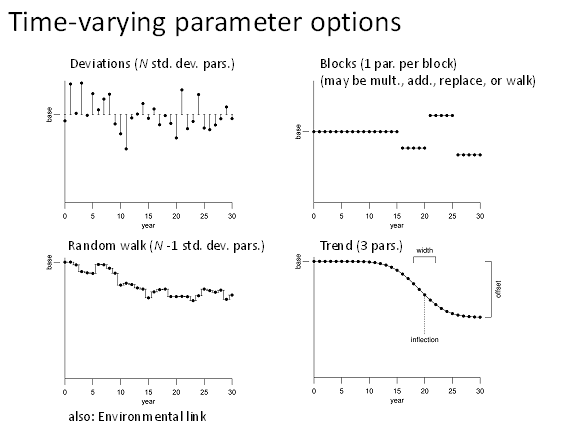
\includegraphics{TimeVarying}
\end{center}
\begin{center}
	\begin{longtable}{p{2.5cm} p{13cm}}
		\hline
		Env var & Values between 100-199, g, causes SS to set the annual working value of this parameter equal to a multiplicative function of Environmental Variable\\
		    & \multicolumn{1}{c}{g: $parm’_y = parm * exp(link * env_{y,g})$ } \\
			& Values between 200-299, g, causes SS to set the annual working value of this parameter equal to a additive function of Environmental Variable g:\\
		    & \multicolumn{1}{c}{ $parm’_y = parm + link * env_{y,g}$}\\
			& Where, link is the environmental link parameter, parm is the base parameter being adjusted, parm’ is the value after adjustment, and env(y-g) is the value of the environmental input g in year y. SS counts the number of parameters that invoke use of an Environmental Variable.  After SS finishes reading the section’s parameter lines, it then creates/reads additional short parameter line(s) to set up the link parameters.  If custom=0, then one short parameter line is used to define the min, max, init, etc, for each of the link parameters.  If custom=1, then a separate line is read for each.\\
		\hline
		Use\_Dev & A value of 1 invokes multiplicative:  $parm’_y = parm * exp(dev_y)$\\
			& A value of 2 invokes additive:  $parm’_y = parm + dev_y$\\
			& A value of 3 invokes additive random walk:  $parm’_y = parm’_{y-1} + dev_y$\\
		    & The vector of devs is simply a vector of offsets; there is no inherent sum to zero constraint.  However, the fact that they are each penalized by the DEV std.dev. below will tend to make them sum towards 0.0.\\
		\hline
		Dev min yr & Beginning year for the dev vector for this parameter\\
		\hline
		Dev max yr & Ending year for the dev vector for this parameter\\
		\hline
		Dev Std Dev. & Standard deviation for elements in the dev vector for this parameter \\
		\hline
		Use Block & Block: A positive value identifies which block pattern will be used for time changes to a parameter value.  Block patterns are simply numbered sequentially as they are defined near the top of the control file, so the index here must be correct for the order in which they are defined.  More than one parameter can use the same block definition.  The order of generated block parameters is by the order of the parameters that call for creation of the block parameters, then by the order of the blocks within that pattern. \\ \\
				  & Trend:  A negative value for the Use\_Block input causes SS to create a parameter time trend instead of blocks.  This time trend requires 3 parameters (instead of the normal one parameter per block).  The base parameter is the value for the adjusted parameter in year = start year.  For subsequent years, the three parameters define a normal distribution of change over time:\\
				  & P1:  parameter value for year = end year.  Either as logistic offset from base P (if Use\_Block=-1), or as direct usage (if Use\_Block=-2)\\
				  & P2:  inflection year;  if HI value for the base parameter is >1.1, then use as year, else use as fraction of range styr - endyr\\
				  & P3:  width of change (units of std.dev. of years)\\
		\hline
		Block Type & This selects the way in which the block parameter creates an offset from the base parameter. \\
				   & 0 means that $parm’ = baseparm * exp(blockparm)$\\
				   & 1 means that $parm’ = baseparm + blockparm$\\
				   & 2 means that $parm’ = blockparm$\\
				   & 3 means that $parm’$ = is additive offset from previous block.  Note that blocks must be contiguous to use this option properly.\\
		\hline
	\end{longtable}
\end{center}

\subsubsection{Parameter Priors}
Priors on parameters fulfill two roles in SS.  First, for parameters provided with an informative prior, SS is receiving additional information about the true value of the parameter.  This information works with the information in the data through the overall logL function to arrive at the final parameter estimate.  Second, diffuse priors provide only weak information about the value of a prior and serve to manage model performance during execution.  For example, some selectivity parameters may become unimportant depending upon the values of other parameters of that selectivity function.  In the double normal selectivity function, the parameters controlling the width of the peak and the slope of the descending side become redundant if the parameter controlling the final selectivity moves to a value indicating asymptotic selectivity.  The width and slope parameters would no longer have any effect on the logL, so they would have no gradient in the logL and would drift aimlessly.  A diffuse prior would then steer them towards a central value and avoid them crashing into the bounds.  Another benefit of diffuse priors is the control of parameters that are given unnaturally wide bounds.  When a parameter is given too broad of a bound, then early in a model run it could drift into this tail and potentially get into a situation where the gradient with respect that parameter approaches zero even though it is not at its global best value.  Here the diffuse prior helps move the parameter back towards the middle of its range where it presumably will be more influential and estimable.  The options for parameter priors are:
\begin{itemize}
	\item -1 = No prior applied.
	\item  0 = Normal prior. Note that this function is independent of the parameter.
	\begin{equation}
		\text{Prior Likelihood} = 0.50*(\frac{Pval - Prior}{Prior\_SD})^2
	\end{equation}
	\item  1 = Symmetric bet prior is scaled between parameter bounds, imposing a larger penalty near the bounds.  Prior standard deviation of 0.05 is very diffuse and a value of 5.0 provides a smooth U-shaped prior.
	\begin{equation}  \mu = -P\_SD*(log((Pmax+Pmin)*0.5-Pmin)-P\_SD*(log(0.5)) \end{equation}
	\begin{equation}
		\begin{split}
			\text{Prior Likelihood} = -(\mu + (P\_SD*(log(Pval-Pmin+Pconst))) + \\
			(P\_SD*(log(1-(\frac{(Pval-Pmin-Pconst)}{(Pmax-Pmin)})))))
		\end{split}
	\end{equation}

	\begin{center}
			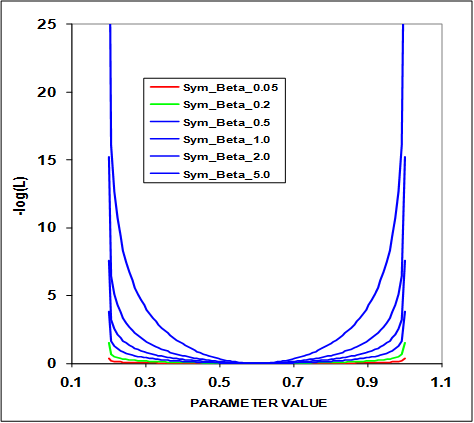
\includegraphics{Beta}\\
			Prior distributions for the symmetric beta distribution.
	\end{center}

	\item 2 = Beta prior.  The definition of $\mu$ is consistent with CASAL's formulation with the Bprior and Aprior corresponding to the m and n parameter.
	\begin{equation}
		\begin{split}
			\mu = \frac{Prior-Pmin}{Pmax-Pmin} \\
			\tau  = \frac{(Prior-Pmin)(Pmax-Prior)}{P\_SD^2}-1.0\\
			Bprior  = \tau*\mu; Aprior = \tau (1.0-\mu)\\
		\end{split}
	\end{equation}
		\begin{equation}
		\begin{split}
		\text{Prior Likelihood} = (1.0-Bprior)*log(Pconst+Pval-Pmin) + \\
		(1.0-Aprior)*log(Pconst+Pmax-Pval) - \\
		(1.0-Bprior)*log(Pconst + Prior - Pmin) - \\
		(1.0-Aprior)*log(Pconst + Pmax - Prior)
		\end{split}
	\end{equation}

	\begin{center}
		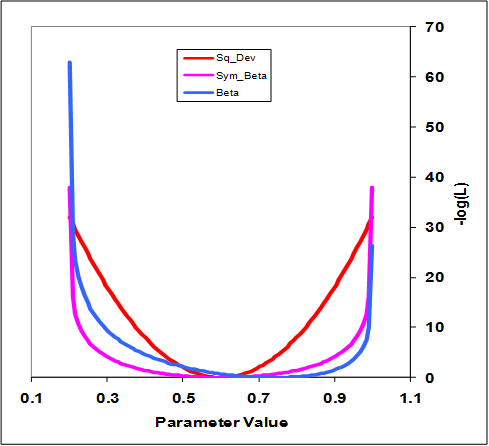
\includegraphics{BetaComparison}\\
		Comparison of the symmetric beta and the beta prior functions
	\end{center}

	\item 3 = Lognormal prior.  Note that lower bound on the parameter must be >0.0. The prior value is input into the parameter line in log space while the initial parameter value is defined in normal space (e.g. INIT = 0.20, PRIOR = -1.609438).
	\begin{equation}
	\text{Prior Likelihood} = 0.50*\Big(\frac{(log(Pval)-Prior)}{Pr\_SD}\Big)^2
	\end{equation}
	\item Pval is the value of the parameter for which a prior is being calculated, Pmin and Pmax are the bounds on the parameter, Prior is the value of the parameter prior, or the first of the 2 factors controlling the calculation of the prior, Pr\_SD is the value of the prior's standard deviation, or the second of the 2 factors controlling the calculation of the prior, Pconst is a small constant (0.0001), and Prior\_Like is the calculated value of the prior's contribution to the log likelihood.
\end{itemize}

		% ======== Section 8: Optional Inputs
		\section{Optional Inputs}

\subsection{Empirical Weight-at-Age (wtatage.ss)}
With version 3.04, SS adds the capability to read empirical body weight at age for the population and each fleet, in lieu of generating these weights internally from the growth parameters, weight-at-length, and size-selectivity.  Selection of this option is done by setting Maturity\textunderscore Option equal to 5.  The values are read from a separate file named, wtatage.ss.  This file is only required to exist if this option is selected.  

The format of this input file is:
\begin{center}
	\begin{tabular}{l l l l l l l l l }
		\hline
		%\multicolumn{2}{l}{10} & \multicolumn{7}{l}{\# Number of rows} \\
		%\hline
		\multicolumn{2}{l}{40} & \multicolumn{7}{l}{\# Number of ages (equal to Maximum Age)} \\
		\hline
		\#Year & Season & Gender & GP & Birth Season & Fleet & Age-0 & Age-1 & ... \\
		\hline
		\-1971 & 1 & 1 & 1 & 1 & 1 & 0.0128586 & 0.13718 & 0.432243 \\
		%\hline
		\-1971 & 1 & 1 & 1 & 1 & 2 & ... & ... & ... \\
		%\hline
		\-1971 & 1 & 1 & 1 & 1 & 0 & ... & ... & ... \\
		%\hline
		-9999 & 1 & 1 & 1 & 1 & 0 & ... & ... & ... \\
		\hline
	\end{tabular}
\end{center}

where:

\begin{itemize}
	\item Fleet = -2 is age-specific fecundity*maturity, so time-varying fecundity is possible to implement
	\item Fleet = -1 is population wt-at-age at middle of the season
	\item Fleet = 0 is population wt-at-age at the beginning of the season
	\item There must be an entry for each fleet for fecundity*maturity, wt-at-age at the middle of the season, and wt-at-age at the beginning of the season.
	\item GP and birthseas probably will never be used, but are included for completeness
	\item A negative value for year will fill the table from that year through the ending year of the forecast, overwriting anything that has already been read for those years.
	\item Judicious use of negative years in the right order will allow user to enter blocks without having to enter a row of info for each year
	\item N ages here equal to maxage specified with the data file, , and N ages +1 columns are required because of age 0 fish.
	\item If N ages in this table is greater than Maxage in the model, the extra wt-at-age values are ignored.
	\item If N ages in this table is less than Maxage in the model, the wt-at-age for N ages is filled in for all unread ages out to Maxage.
	\item There is no internal error checking to  verify that weight-at-age has been read for every fleet and every year. 
	\item Fleets that do not use biomass do not need to have wt-at-age assigned	
	\item The values entered for endyr+1 will be used for the benchmark calculations and for the forecast; this aspect needs a bit more checking
\end{itemize}

CAVEATS:
\begin{itemize}
	\item SS will still calculate growth curves from the input parameters and can still calculate size-selectivity and can still examine size composition data.
	\item However, there is no calculation of wt-at-age from the growth input, so no way to compare the input wt-at-age from the wt-at-age derived from the growth parameters.
	\item If wt-at-age is read and size-selectivity is used, a warning is generated
	\item If wt-at-age is read and discard/retention is invoked, then a BEWARE warning is generated because of untested consequences for the body wt of discarded fish.
	\item Warning:  age 0 fish seem to need to have weight=0 for spawning biomass calculation (code -2).
\end{itemize}

TESTING:
\begin{itemize}
	\item A model was setup with age-maturity (option 2) and only age selectivity.
	\item The output calculation of wt-at-age and fecundity-at-age was taken from report.sso and put into wtatage.ss (as shown above).
	\item Re-running SS with this input wt-at-age (Maturity\textunderscore Option 5) produced identical results to the run that had generated the weight-at-age from the growth parameters.
\end{itemize}

\subsection{runnumbers.ss}
This file contains a single integer value.  It is read when the program starts, incremented by 1, used when processing the profile value inputs (see below), used as an identifier in the batch output, then saved with the incremented value.  Note that this incrementation may not occur if a run crashes.

\subsection{profilevalues.ss}	
This file contains information for changing the value of selected parameters for each run in a batch.  In the ctl file, each parameter that will be subject to modification by profilevalues.ss is designated by setting its phase to --9999 .

The first value in profilevalues.ss is the number of parameters to be batched.  This value MUST match the number of parameters with phase set equal to -9999 in the ctl file.  The program performs no checks for this equality.  If the value is zero in the first field, then nothing else will be read.  Otherwise, the model will read runnumber * Nparameters values and use the last Nparameters of these to replace the initial values of parameters designated with phase = --9999 in the ctl file.

USAGE Note:  
If one of the batch runs crashes before saving the updated value of runnumber.ss, then the processing of the profilevalue.ss will not proceed as expected.  Check the output carefully until a more robust procedure is developed.



		% ======== Section 11: Output Files
		\section{Output Files}
\subsection{Standard ADMB output files}
Standard ADMB files are created by SS.  These are:\\
\\
SS.PAR – This file has the final parameter values.  They are listed in the order they are declared in SS.  This file can be read back into SS to restart a run with these values (see running SS).\\
\\
SS.STD – This file has the parameter values and their estimated standard deviation for those parameters that were active during the model run.  It also contains the derived quantities declared as sdreport variables.  All of this information is also report in the covar.sso.  Also, the parameter section of report.sso lists all the parameters with their SS generated names, denotes which were active in the reported run, displays the parameter standard deviations, then displays the derived quantities with their standard deviations.\\
\\
SS.REP – This report file is created between phases so, unlike report.sso, will be created even if the Hessian fails.  It does not contain as much output as shown in report.sso.\\
\\
SS.COR – This is the standard ADMB report for parameter and sdreport correlations.  It is in matrix form and challenging to interpret.  This same information is reported in covar.sso.

\subsection{SS Summary}
The ss\_summary.sso file (available for versions 3.30.08.03 and later) is designed to put key model outputs all in one concise place.  It is organized as a list.  At the top of the file are some descriptors, followed by the likelihoods for each component, then the parameters and their standard errors, then the derived quantities and their standard errors.  This output was created to make it easy to compare the results between different versions of the executable, however, this file could be useful for numerous other uses. 

\subsection{SIS table}
The SIS\_table.sso file contains model output formatted for reading into the NMFS Species Information System.

\subsection{Derived Quantities}
Before listing the derived quantities reported to the sdreport, there are a couple of topics that deserve further explanation.

\subsubsection{Metric for Fishing Mortality}
A generic single metric of annual fishing mortality is difficult to define in a generalized model that admits multiple areas, multiple biological cohorts, dome-shaped selectivity in size and age for each of many fleets.  Several separate indices are provided and others could be calculated by a user from the detailed information in report.sso.

\subsubsection{Equilibrium SPR}
This index focuses on the effect of fishing on the spawning potential of the stock.  It is calculated as the ratio of the equilibrium reproductive output per recruit that would occur with the current year’s F intensities and biology, to the equilibrium reproductive output per recruit that would occur with the current year’s biology and no fishing.  Thus it internalizes all seasonality, movement, weird selectivity patterns, and other factors.  Because this index moves in the opposite direction than F intensity itself, it is usually reported as 1-SPR.  A benefit of this index is that it is a direct measure of common proxies used for F\textsubscript{MSY}, such as F\textsubscript {40\%}.  A shortcoming of this index is that it does not directly demonstrate the fraction of the stock that is caught each year.  The SPR value is also calculated in the benchmarks (see below).  The derived quantities report shows an annual SPR statistic.  The options, as specified in the starter.ss file, are:
\begin{itemize}
	\item 0 = skip
	\item 1 = (1-SPR)/(1-SPR\textsubscript{TGT})
	\item 2 = (1-SPR)/(1-SPR\textsubscript{MSY})
	\item 3 = (1-SPR)/(1-SPR\textsubscript{Btarget})
	\item 4 = raw SPR
\end{itemize}

\subsubsection{F std}
This index provides a direct measure of fishing mortality.  The options are:
\begin{itemize}
	\item 0 = skip
	\item 1 = exploitation(Bio)
	\item 2 = exploitation(Num)
	\item 3 = sum(Frates)
\end{itemize}
The exploitation rates are calculated as the ratio of the total annual catch (in either biomass or numbers as specified) to the summary biomass or summary numbers on Jan 1.  The sum of the F rates is simply the sum of all the apical Fs.  This makes sense if the F method is in terms of instantaneous F (not Pope’s approximation) and if there are not fleets with widely different size/age at peak selectivity, and if there is no seasonality, and especially if there is only one area.  In the derived quantities, there is an annual statistic that is the ratio of the can be annual F\_std value to the corresponding benchmark statistic.  The available options for the denominator are:
\begin{itemize}
	\item 0 = raw
	\item 1 = F/F\textsubscript {SPR}
	\item 2 = F/F\textsubscript {MSY}
	\item 3 = F/F\textsubscript {Btarget}
\end{itemize}

\subsubsection{F-at-Age}
Because the annual F is so difficult to interpret as a sum of individual F components, an indirect calculation of F-at-age is reported at the end of the report.sso file.  This section of the report calculates Z-at-age simply as $ln(N_{a+1,t+1}/N_{a,t})$.  This is done on an annual basis and summed over all areas.  It is done once using the fishing intensities as estimated (to get Z), and once with the F intensities set to 0.0 to get M-at-age.  This latter sequence also provides a measure of dynamic Bzero.  The user can then subtract the table of M-at-age/year from the table of Z-at-age/year to get a table of F-at-age/year.  From this apical F, average F over a range of ages, or other user-desired statistics could be calculated.  Further work within SS with this table of values is anticipated.

\subsubsection{MSY and other Benchmark Items}
The following quantities are included in the sdreport vector mgmt\_quantities, so obtain estimates of variance.  Some additional quantities can be found in the benchmarks section of the forecast\_report.sso.

\begin{center}
	\begin{longtable}{p{4cm} p{11cm}}
		Benchmark Item &  Description\\
		\hline
		\endfirsthead


		Benchmark Item &  Description\\
		\hline
		\endhead
		
		\endfoot
		\hline		
		\endlastfoot
		
		SSB\_Unfished & Unfished reproductive potential (SSB is commonly female mature spawning biomass)\\
		TotBio\_Unfished & Total age 0+ biomass on Jan 1\\
		SmryBio\_Unfished & Biomass for ages at or above the summary age on Jan 1\\
		Recr\_Unfished & Unfished recruitment\\
		SSB\_Btgt & SSB at user specified SSB target\\
		SPR\_Btgt & Spawner potential ratio (SPR) at F intensity that produces user specified SSB target\\
		Fstd\_Btgt & F statistic at F intensity that produces user specified SSB target\\
		TotYield\_Btgt & Total yield at F intensity that produces user specified SSB target\\
		SSB\_SPRtgt & SSB at user specified SPR target (but taking into account the spawner-recruitment relationship)\\
		Fstd\_SPRtgt & F intensity that produces user specified SPR target\\
		TotYield\_SPRtgt & Total yield at F intensity that produces user specified SPR target\\
		SSB\_MSY & SSB at F intensity that is associated with MSY; this F intensity may be directly calculated to produce MSY, or can be mapped to F\_SPR or F\_Btgt\\
		SPR\_MSY & Spawner potential ratio (SPR) at F intensity associated with MSY\\
		Fstd\_MSY & F statistic at F intensity associated with MSY\\
		TotYield\_MSY & Total yield (biomass) at MSY \\
		RetYield\_MSY & Retained yield (biomass) at MSY 
	\end{longtable}
\end{center}

\subsection{Brief cumulative output}
Cum\_Report.sso:  contains a brief version of the run output, which is appended to current content of file so results of several runs can be collected together.  This is especially useful when a batch of runs is being processed.  Unless this file is deleted, it will contain a cumulative record of all runs done in that subdirectory.  The first column contains the run number.  

\subsection{Output for Rebuilder Package}
Output filename is REBUILD.DAT\\
\\
\#Title  \# various run summary outputs\\
SS\#\_default\_rebuild.dat\\
\# Number of sexes\\
2\\
\# Age range to consider (minimum age; maximum age)\\
0 40\\
\# Number of fleets\\
3\\
\# First year of projection (Yinit)\\
2002\\
\# First Year of rebuilding period (Ydecl)\\
1999\\
\# Number of simulations\\
1000\\
\# Maximum number of years\\
500\\
\# Conduct proejctions with multiple starting values (0 = No, 1 = Yes)\\
0\\
\# Number of parameter vectors\\
1000\\
\# Is the maximum age a plus-group (1 = Yes; 2 = No)\\
1\\
\#Generate future recruitments using historical recruitments (1) historical recruits/spawner (2)  or a stock-recruitment (3)\\
3\\
\# Constant fishing mortality (1) or constant Catch (2) projections\\
1\\
\# Fishing mortality based on SPR (1) or actual rate (2)\\
1v
\# Pre-specify the year of recovery (or -1) to ignore\\
-1\\
\# Fecundity-at-age\\
\# 0 1 2 3 4 5 6 7 8 9 10 <deleted values> \\
0 0.000450117 0.00436298 0.0271371 <deleted values> \\
\# Age specific selectivity and weight adjusted for discard and discard mortality\\
\#wt and selex for gender, fleet: 1 1\\
0.146708 0.320119 0.555587 0.830467 <deleted values> \\
0.0122887 0.0351722 0.0838682 0.165479 <deleted values> \\
\#wt and selex for gender ,fleet: 2 1\\
0.150944 0.33768 0.588317 0.874376 <deleted values>\\
0.0127241 0.0380999 0.0922667 <deleted values>\\
\# M and current age-structure in year Yinit: 2002\\
\# gender = 1\\
0.1 0.1 0.1 0.1 0.1 <deleted values>\\
1425.96 797.624 1234.77 428.207 <deleted values>\\
\# gender = 2\\
0.1 0.1 0.1 0.1 0.1 <deleted values>\\
1425.96 797.531 1233.66 <deleted values> \\
\# Age-structure at Ydeclare= 1999\\
598.671 652.739 2925.76 2227.69 <deleted values>\\
598.671 652.666 2923.27 2221.05 <deleted values>\\
\# Year for Tmin Age-structure (set to Ydecl by SS) 1999\\
1999\\
\#  recruitment and biomass\\
\# Number of historical assessment years\\
33\\
\# Historical data\\
\# year recruitment spawner in B0 in R project in R/S project\\
1970 1971 1972 1973 1974 1975 1976 <deleted values> 2001 2002 \\
\#years (with first value representing R0)\\
8853.43  8658.22 8651.96 8645.41 8638.43 8630.75 <deleted values> 1594.53 2075.34 \#recruits; first value is R0 (virgin)\\
63679.5  63679.5 63679.3 63678.3 63673.9 63661.6 <deleted values> 8614.18 7313.2 \#spbio; first value is S0 (virgin)\\
1 0 0 0 0 0 0 0 0 0 0 0 0 0 0 0 0 0 0 0 0 0 0 <deleted values> 0 0  \# in Bzero\\
0 1 1 1 1 1 1 <deleted values> 1 1  0 0 0 \# in R project\\
0 1 1 1 1 1 1 <deleted values> 1 1  0 0 0 \# in R/S project\\
\# Number of years with pre-specified catches\\
0\\
\# catches for years with pre-specified catches go next\\
\# Number of future recruitments to override\\
3\\
\# Process for overriding (-1 for average otherwise index in data list)\\
2000 1 2000\\
2001 1 2001\\
2002 1 2002\\
\# Which probability to product detailed results for (1=0.5; 2=0.6; etc.)\\
3\\
\# Steepness sigma-R Auto-correlation\\
0.610789 0.6 0 \\
\# Target SPR rate (FMSY Proxy); manually change to SPR\_MSY if not using SPR\_target\\
0.5\\
\# Target SPR information: Use (1=Yes) and power\\
0 20\\
\# Discount rate (for cumulative catch)\\
0.1\\
\# Truncate the series when 0.4B0 is reached (1=Yes)\\
0\\
\# Set F to FMSY once 0.4B0 is reached (1=Yes)\\
0\\
\# Maximum possible F for projection (-1 to set to FMSY)\\
-1\\
\# Defintion of recovery (1=now only; 2=now or before)\\
2\\
\# Projection type\\
4\\
\# Definition of the 40-10 rule\\
10 40\\
\# Produce the risk-reward plots (1=Yes)\\
0\\
\# Calculate coefficients of variation (1=Yes)\\
0\\
\# Number of replicates to use\\
10\\
\# Random number seed\\
-99004\\
\# File with multiple parameter vectors \\
rebuild.SS0\\
\# User-specific projection (1=Yes); Output replaced (1->9)\\
0  5  \\
\# Catches and Fs (Year; 1/2/3 (F or C or SPR); value); Final row is -1v
2002 1 1\\
-1 -1 -1\\
\# Split of Fs\\
2002 1\\
-1  1 1 1\\ 
\# Yrs to define TTARGET for projection type 4 (aka 5 pre-specified inputs)\\
2011 2012 2013 2014 2015 2016 2017 2018 \\
\# Time varying weight-at-age (1=Yes;0=No)\\
0\\
\# File with time series of weight-at-age data\\
none\\
\# Use bisection (0) or linear interpolation (1)\\
1\\
\# Target Depletion\\
0.4\\
\# CV of implementation error\\
0\\

\subsection{Bootstrap Data Files}
Data.ss\_new:  contains a user-specified number of data files, generated through a parametric bootstrap procedure, and written sequentially to this file.  These can be parsed into individual data files and re-run with the model.  The first output provides the unaltered input data file (with annotations added).  The second provides the expected values for only the data elements used in the model run.  The third and subsequent outputs provide parametric bootstraps around the expected values.

\subsection{Forecast and Reference Points}
FORECAST-REPORT.sso:  This file contains output of fishery reference points and forecasts.  It is designed to meet the needs of the Pacific Fishery Management Council’s Groundfish Fishery Management Plan, but it should be quite feasible to develop other regionally specific variants of this output.

The vector of forecast recruitment deviations is estimated during an additional model estimation phase.  This vector includes any years after the end of the recrdev time series and before or at the end year.  When this vector starts before the ending year of the time series, then the estimates of these recruitments will be influenced by the data in these final years.  This is problematic, because the original reason for not estimating these recruitments at the end of the time series was the poor signal/noise ratio in the available data.  It is not that these data are worse than data from earlier in the time series, but the low amount of data accumulated for each cohort allows an individual datum to dominate the model’s fit.  Thus, an additional control is provided so that forecast recruitment deviations during these years can receive an extra weighting in order to counter-balance the influence of noisy data at the end of the time series.

An additional control is provided for the fraction of the log-bias adjustment to apply to the forecast recruitments.  Recall that R is the expected mean level of recruitment for a particular year as specified by the spawner-recruitment curve and R’ is the geometric mean recruitment level calculated by discounting R with the log-bias correction factor e-0.5s\^2.  Thus a lognormal distribution of recruitment deviations centered on R’ will produce a mean level of recruitment equal to R.  During the modeled time series, the virgin recruitment level and any recruitments prior to the first year of recruitment deviations are set at the level of R, and the lognormal recruitment deviations are centered on the R’ level.  For the forecast recruitments, the fraction control can be set to 1.0 so that 100\% of the log-bias correction is applied and the forecast recruitment deviations will be based on the R’ level.  This is certainly the configuration to use when the model is in MCMC mode.   Setting the fraction to 0.0 during maximum likelihood forecasts would center the recruitment deviations, which all have a value of 0.0 in ML mode, on R.  Thus would provide a mean forecast that would be more comparable to the mean of the ensemble of forecasts produced in MCMC mode.  Further work on this topic is underway.\\
\\
Note:
\begin{itemize}
	\item Cohorts continue growing according to their specific growth parameters in the forecast period rather than staying static at the endyr values.
	\item Environmental data entered for future years can be used to adjust expected recruitment levels.  However, environmental data will not affect growth or selectivity parameters in the forecast.
\end{itemize}

The top of this file shows the search for F\textsubscript {SPR}  and the search for F\textsubscript {MSY}  so the user can verify convergence.  Note:  if the STD file shows aberrant results, such as all the standard deviations being the same value for all recruitments, then check the F\textsubscript {MSY}  search for convergence. 

The F\textsubscript {MSY} can be calculated, or set equal to one of the other F reference points per the selection made in STARTER.SS.

The reference point output is shown int he table below: 
\begin{center}
	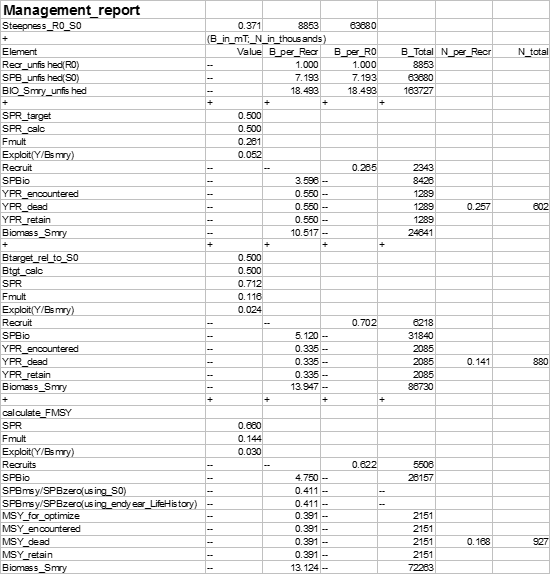
\includegraphics{ManagementReport}
\end{center}


\begin{landscape}
	The forecast is done once using the Target SPR and once using the adjustments specified in the 40:10 section of forecast.ss input.  Each section contains a time series of seasonal biomass and catch, followed by a time series of population numbers-at-age for each platoon.
	
	\begin{center}
		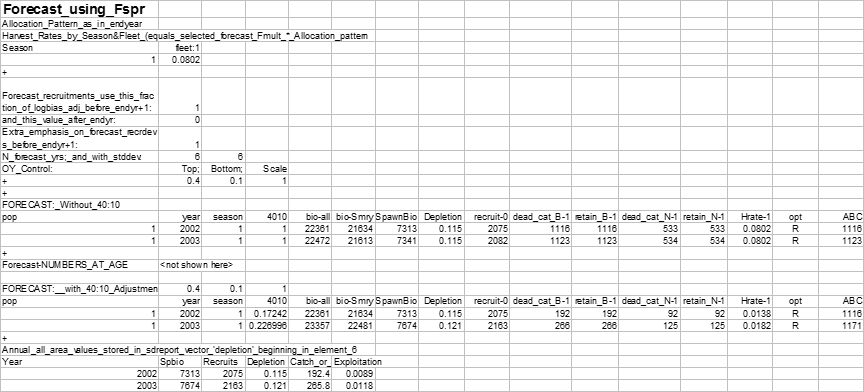
\includegraphics{Forecast}
	\end{center}
\end{landscape}

where:
\begin{itemize}
	\item 40:10 is the magnitude of the adjustment of harvest multiplier to implement the OY policy
	\item bio-all is the biomass of all ages
	\item bio-smry is the biomass for ages at or above the summary age
	\item Spawnbio - is the female spawning output
	\item Depletion is the spawnbio divided by the unfished spawnbio
	\item Recruit-0 is the recruitment of age-o fish in this year
	\item Dead\_cat\_B-1 is the total dead (retained plus dead discard) catch in MT for fleet 1
	\item Retain\_B-1 is fleet 1’s retained catch in MT
	\item Equivalent catch in numbers is then reported.
	\item Hrate-1 is the harvest rate, as adjusted by the 40:10 policy.  The units will depend on the F method selected (Pope’s method giving mid-year harvest rate or the continuous F.
	\item Opt=C means that the rate was calculated from an input catch level (and crashed means that this caused an excessive harvest rate.
	\item Opt=R means that the catch was calculated from the target harvest rate.
	\item ABC is equal to the Total-Catch when the 40:10 option is not used (upper portion of table).  When the 40:10 is on (lower table), the ABC is the catch level corresponding to no 40:10 adjustment after accounting for catch in previous year’s from the 40:10.
\end{itemize}

The time series output described above is detailed by season, area, platoon and fishery.  It is usually more convenient to have annual values summed across areas, platoons and fisheries.  This is done for the 40:10 output and a subset of these values are replicated in the depletion vector in the sd\_report so that variance estimates can be obtained.  The elements of the depletion vector in the sd\_report are:
\begin{itemize}
	\item depletion level in end year
	\item depletion level in end year+1
	\item MSY (if calculated, else spbio in endyr-1)
	\item B\textsubscript{MSY} (if calculated, else spbio in endyr)
	\item SPR\textsubscript{MSY} (if calculated, else spbio in endyr+1) then the time series of:
	\begin{itemize}
		\item Spawning biomass
		\item Recruitment
		\item Depletion level
		\item Total catch (if forecast calculated catch from rates) or sum of fishery-specific harvest rates (if forecast is based on fixed input catch level in this year)
		\item Total exploitation rate (total dead catch divided by the summary biomass at the beginning of the year).
	\end{itemize}
\end{itemize}

\begin{center}
	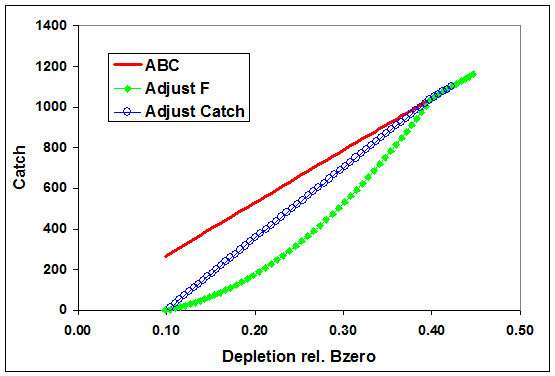
\includegraphics{HCR}\\
	Two examples of harvest forecast adjustment: one adjusts catch and the other adjusts F.
\end{center}

\subsection{Main Output File, report.sso}
This is the primary output file.  Its major sections are listed below.  

The sections of the output file are:
\begin{itemize}
	\item SS version number with date compiled.  Time and date of model run.  This info appears at the top of all output files.
	\item Comments
		\begin{itemize}
			\item 	Input file lines starting with \#C are echoed here
		\end{itemize}
	\item Keywords
		\begin{itemize}
			\item List of keywords used in searching for output sections.
		\end{itemize}
	\item Fleet Names
		\begin{itemize}
			\item List of fishing fleet and survey names assigned in the data file
		\end{itemize}
	\item Likelihood
		\begin{itemize}
			\item Final values of the negative log(likelihood) are presented.
		\end{itemize}
	\item Input Variance Adjustments
		\begin{itemize}
			\item The matrix of input variance adjustments is output here because these values affect the logL calculations
		\end{itemize}
	\item Parameters
		\begin{itemize}
			\item The parameters are listed here.  For the estimated parameters, the display shows: Num (count of parameters), Label (as internally generated by SS), Value, Active\_Cnt, Phase, Min, Max, Init, Prior, Prior\_type, Prior\_SD, Prior\_Like, Parm\_StD (standard deviation of parameter as calculated from inverse Hessian), Status (e.g. near bound), Pr\_atMin (value of prior penalty if parameter was near bound), and  Pr\_atMin.  The Active\_Cnt entry is a count of the parameters in the same order they appear in the ss.cor file.
		\end{itemize}
	\item Derived Quantities
		\begin{itemize}
			\item This section starts by showing the options selected from the starter.ss and forecast.ss input files:
				\begin{itemize}
					\item SPR ratio basis
					\item F report basis
					\item B ratio denominator
				\end{itemize}
		\end{itemize}
\end{itemize}

Then the time series of output, with standard deviation of estimates, are produced with internally generated labels.  Note that these time series extend through the forecast era.  The order of the output is:  spawning biomass, recruitment, SPRratio, Fratio, Bratio, management quantities, forecast catch (as a target level), forecast catch as a limit level (OFL), Selex\_std, Grow\_std, NatAge\_std.  For the three “ratio” quantities, there is an additional column of output showing a Z-score calculation of the probability that the ratio differs from 1.0.  The “management quantities” section is designed to meet the terms of reference for west coast groundfish assessments; other formats could be made available upon request.  The std quantities at the end are set up according to specifications at the end of the control input file.  In some cases, a user may specify that no derived quantity output of a certain type be produced.  In those cases, SS substitutes a repeat output of the virgin spawning biomass so that vectors of null length are not created.

ADMB NOTE:  while vectors of null length are very useful for controlling optional model inputs, they cannot be used with current version of ADMB for sdreport quantities.

\begin{itemize}
	\item MGparm by year after adjustments
	\begin{itemize}
		\item This block shows the time series of Mgparms by year after adjustment by environmental links, blocks and deviations.
	\end{itemize}
	\item SELparm (size) by year after adjustments
	\begin{itemize}
		\item This block shows the size selectivity parameters, after adjustment, for each year in which a change occurs.
	\end{itemize}
	\item SELparm (age) by year after adjustments
	\begin{itemize}
		\item This block shows the age selectivity parameters, after adjustment, for each year in which a change occurs.
	\end{itemize}
	\item Recruitment Distribution
	\begin{itemize}
		\item This block shows the distribution of recruitment across growth patterns, genders, birthseasons, and areas in the endyr of the model.
	\end{itemize}
	\item Platoon Indexing
	\begin{itemize}
		\item This block shows the internal index values for various quantities.  It can be a useful reference for complex model setups.  The vocabulary is:  Bio\_Pattern refers to a collection of cohorts with the same defined growth and natural mortality parameters; sex is the next main index.  If recruitment occurs in multiple seasons, then Birthseas is the index for that factor.  The index labeled “Platoon” is used as a continuous index across all the other factor-specific indices.  If sub-platoons are used, they are nested within the Bio\_Pattern x Sex x Birthseas platoon.  However, some of the output tables use the column label “platoon” as a continuous index across platoons and sub-platoons.  Note that there is no index here for area.  Each of the cohorts is distributed across areas and they retain their biological characteristics as they move among areas.
	\end{itemize}
	\item Size Freq Translation
	\begin{itemize}
		\item If the generalize size frequency approach is used, this block shows the translation probabilities between population length bins and the units of the defined size frequency method.  If the method uses body weight as the accumulator, then output is in corresponding units.
	\end{itemize}
	\item Movement
	\begin{itemize}
		\item This block shows movement rate between areas in a multi-area model.
	\end{itemize}
	\item Exploitation
	\begin{itemize}
		\item This block shows the time series of the selected F\_std unit and the F multiplier for each fleet in terms of harvest rate (if Pope’s approximation is used) or fully selected F.
	\end{itemize}
	\item Index 2
	\begin{itemize}
		\item This section reports the observed and expected values for each index.  All are reported in one list with index number included as a selection field.  At the bottom of this section, the root mean squared error of the fit to each index is compared to the mean input error level to assist the user in gaging the goodness-of-fit and potentially adjusting the input level of imprecision.
	\end{itemize}
	\item Index 3
	\begin{itemize}
		\item This section shows the parameter number assigned to each parameter used in this section.
	\end{itemize}
	\item Discard
	\begin{itemize}
		\item This is the list of observed and expected values for the amount (or fraction) discard.
	\end{itemize}
	\item Mean Body Wt
	\begin{itemize}
		\item This is the list of observed and expected values for the mean body weight.
	\end{itemize}
	\item Fit Len Comps
	\begin{itemize}
		\item This is the list of the goodness of fit to the length compositions.  The input and output levels of effective sample size are shown as a guide to adjusting the input levels to better match the model’s ability to replicate these observations.
	\end{itemize}
	\item Fit Age Comps
	\begin{itemize}
		\item This has the same format as the length composition section.
	\end{itemize}
	\item Fit Size Comps
	\begin{itemize}
		\item This has the same format as the length composition section and is used for the generalized size composition summary.
	\end{itemize}
	\item Len Selex
	\begin{itemize}
		\item Here is the length selectivity and other length specific quantities for each fishery and survey.
	\end{itemize}
	\item Age Selex
	\begin{itemize}
		\item Here is reported the time series of age selectivity and other age-related quantities for each fishery and survey.  Some are directly computed in terms of age, and others are derived from the combination of a length-based factor and the distribution of size-at-age.
	\end{itemize}
	\item Environmental Data
	\begin{itemize}
		\item The input values of environmental data are echoed here.  In the future, the summary biomass in the previous year will be mirrored into environmental column –2 and that the age zero recruitment deviation into environmental column –1.  Once so mirrored, they may enable density-dependent effects on model parameters.
	\end{itemize}
	\item Numbers at Age
	\begin{itemize}
		\item The output (in thousands of fish) is shown for each cohort tracked in the model.
	\end{itemize}
	\item Numbers at Length
	\begin{itemize}
		\item The output is shown for each cohort tracked in the model.
	\end{itemize}
	\item Catch at Age
	\begin{itemize}
		\item The output is shown for each fleet.  It is not necessary to show by area because each fleet operates in only one area.
	\end{itemize}
	\item Biology
	\begin{itemize}
		\item The first biology section shows the length-specific quantities in the ending year of the time series only.  The derived quantity spawn is the product of female body weight, maturity and fecundity per weight.  The second section shows natural mortality.
	\end{itemize}
	\item Growth Parameters
	\begin{itemize}
		\item This section shows the growth parameters, and associated derived quantities, for each year in which a change is estimated.
	\end{itemize}
	\item Biology at Age
	\begin{itemize}
		\item This section shows derived size-at-age and other quantities.  It is the basis for the Bio report page of the Excel output processor.
	\end{itemize}
	\item Mean Body Wt (begin)
	\begin{itemize}
		\item This section reports the time series of mean body weight for each platoon.  Values shown are for the beginning of each season of each year.
	\end{itemize}
	\item Mean Size Timeseries
	\begin{itemize}
		\item This section shows the time series of mean length-at-age for each platoon.  At the bottom is the average mean size as the weighted average across all platoons for each gender.
	\end{itemize}
	\item Age Length Key
	\begin{itemize}
		\item This is reported for the midpoint of each season in the ending year.
	\end{itemize}
	\item Age Age Key
	\begin{itemize}
		\item This is the calculated distribution of observed ages for each true age for each of the defined ageing keys.
	\end{itemize}
	\item Selectivity Database
	\begin{itemize}
		\item This section contains the selectivities organized as a database, rather than as a set of vectors.
	\end{itemize}
	\item Spawning Biomass Report 2, etc.
	\begin{itemize}
		\item The section shows annual total spawning biomass, then numbers-at-age at the beginning of each year for each Bio\_Pattern and Sex as summed over sub-platoons and areas.  Then Z-at-age is reported simply as $ln(N_{t+1,a+1} N_{t,a})$.  Then the Report\_1 section loops back through the time series with all F values set to zero so that a dynamic Bzero, N-at-age, and M-at-age can be reported.  The difference between Report\_1 and Report\_2 can be used to create an aggregate F-at-age.
	\end{itemize}
	\item Composition Database
	\begin{itemize}
		\item This section is reported to a separate file, compreport.sso, and contains the length composition, age composition, and mean size-at-age observed and expected values.  It is arranged in a database format, rather than an array of vectors.  Software to filter the output allows display of subsets of the database.
	\end{itemize}
\end{itemize}

		%========= Section 12: Running SS
		\section{Running SS} \label{sec:RunningSS}

\subsection{Command Line Interface}
The name of the SS executable files often contains the phrase "safe" or "opt" (for optimized). The safe version includes checking for out of bounds values and should always be used whenever there is a change to the data file. The optimized version runs slightly faster but can result in data not being included in the model as intended if the safe version has not been run first. A file named "ss.exe" is typically the safe version unless the result of renaming by the user. In some situations, users may wish to rename the file they are using to ss.exe, but the longer file name can be used.

On Mac and Linux computers, the executable does not include an extension (like .exe on Windows).
Running the executable on from the DOS command line in Windows simply require typing the executable name (without the .exe extension):
\begin{quote}
	\begin{verbatim}
	> ss
	\end{verbatim}
\end{quote}


On Mac and Linux computers, the executable name must be preceded by a period and slash (unless it's location has been added to the user's PATH):

\begin{quote}
	\begin{verbatim}
	> ./ss
	\end{verbatim}
\end{quote}


Additional ADMB commands can follow the executable name, such as "–nohess" to avoid calculating the Hessian matrix. To see a full list of options, add " -?" after the executable name (with a space in between).

On all operating systems, a copy of the SS executable can either be located in the same directory as the model input files or in a central location and referenced either by adding it to the PATH or by a script files. Further discussion on script files for Windows is below. Editing the PATH is not covered here.


\subsubsection{Example of DOS batch input file}
One file management approach is to put ss.exe in its own folder (example:  C:\textbackslash SS\_model) and to put your input files in separate folder (example:  C:\textbackslash My Documents \textbackslash SS\_runs).  Then a DOS batch file in the SS\_runs folder can be run at the command line to start ss.exe.  All output will appear in SS\_runs folder.

A DOS batch file (e.g. SS.bat) might contain some explicit ADMB commands, some implicit commands, and some DOS commands:

\begin{quote}
	\begin{verbatim}
	c:\SS_model\ss.exe -cbs 5000000000 -gbs 50000000000 \%1 \%2 \%3 \%4 
	del ss.r0*
	del ss.p0*
	del ss.b0*
	\end{verbatim}
\end{quote}


In this batch file, the –cbs and –gbs arguments allocate a large amount of memory for SS to use (you may need to edit these for your computer and SS configuration), and the \%1, \%2 etc. allows passing of command line arguments such as –nox or –nohess.  You add more items to the list of \% arguments as needed.

An easy way to start a command line in your current directory (SS\_runs) is to create a shortcut to the DOS command line prompt.  The shortcut’s target would be:

\begin{quote}
	\begin{verbatim}
	> %SystemRoot%\system32\cmd.exe
	\end{verbatim}
\end{quote}


\noindent And it would start in:
\begin{quote}
	\begin{verbatim}
	> %CURRDIR%
	\end{verbatim}
\end{quote}

An alternative shortcut is to have the executable within the model folder then use Ctrl+Shift+Right Click and then select either "Open powershell window here" or "Open command window here", depending upon your computer.  From the command window the executable name can be typed along with additional inputs (e.g., -nohess) and the model run.  If using the powershell type cmd and then hit enter prior to calling the model (ss). 


\subsubsection{Simple Batch}
This first example relies upon having a set of prototype files that can be renamed to starter.ss and then used to direct the running of SS.  The example also copies one of the output files to save it from being overwritten.  This sequence is repeated 3 times here and can be repeated an unlimited number of times.  The batch file can have any name with the .bat extension, and there is no particular limit to the DOS commands invoked.  Note that brief output from each run will be appended to cumreport.sso (see below).

\begin{quote}
	\begin{verbatim}
	del ss.cor
	del ss.std
	copy starter.r01 starter.ss
	c:\admodel\ss\ss.exe -sdonly
	copy ss.std ss-std01.txt
	copy starter.r01 starter.ss
	c:\admodel\ss\ss.exe -sdonly
	copy ss.std ss-std02.txt
	\end{verbatim}
\end{quote}


\subsubsection{Complicated Batch}
This second example processes 25 dat files from a different directory, each time using the same ctl and nam file.  The loop index is used in the file names, and the output is searched for particular keywords to accumulate a few key results into the file SUMMARY.TXT.  Comparable batch processing can be accomplished by using R or other script processing programs.

\begin{quote}
	\begin{verbatim}
	del summary.txt
	del ss-report.txt
	copy /Y runnumber.zero runnumber.ss
	FOR /L \%\%i IN (1,1,25) DO (
	copy /Y ..\MakeData\A1-D1-%%i.dat  Asel.dat
	del ss.std
	del ss.cor
	del ss.par
	c:\admodel\ss\ss.exe
	copy /Y ss.par A1-D1-A1-%%i.par
	copy /Y ss.std A1-D1-A1-%%i.std
	find "Number" A1-D1-A1-%%i.par >> Summary.txt
	find "hessian" ss.cor >> Summary.txt)
	\end{verbatim}
\end{quote}



\subsubsection{Running Parameter Profiles}
Users will often want to run profiles over specific parameter to evaluate the information in the model to estimate the parameter based on changes in the log likelihood.  There are two ways this can be done.

The first option is the use functions within \texttt{r4ss} to run the profile, summarize quantities across runs, and plot the output.  The \texttt{SS\_profile()} function will run the profile based on function inputs, \texttt{SSgetoutput()} will read quantities from each run Report file, \texttt{SSsummarize()} will summarize key model quantities, and the \texttt{SSplotProfile()} and \texttt{PinerPlot()} functions can be used to visualize results.  Additional information regarding \texttt{r4ss} can be found on page \pageref{r4ss}. 

The second way is to create and run a batch file to profile over parameters. This example will run a profile on natural mortality and spawner-recruitment steepness, of course.  Edit the control file so that the natural mortality parameter and steepness parameter lines have the phase set to –9999.  Edit STARTER.SS to refer to this control file and the appropriate data file.

%\begin{center}
	\begin{longtable}{p{0.5cm} p{16cm}}		
		& Create a PROFILEVALUES.SS file\\
		& 2	\# number of parameters using profile feature\\
		& 0.16	\# value for first selected parameter when runnumber equals 1\\
		& 0.35	\# value for second selected parameter when runnumber equals 1\\
		& 0.16	\# value for first selected parameter when runnumber equals 2\\
		& 0.40	\# value for second selected parameter when runnumber equals 2\\
		& 0.18	\# value for first selected parameter when runnumber equals 3\\
		& 0.40	\# value for second selected parameter when runnumber equals 3\\
		& etc.;  make it as long as you like.\\
	\end{longtable}

Create a batch file that looks something like this.  Or make it more complicated as in the example above.


\begin{quote}
\begin{verbatim}
	del cumreport.sso
	copy /Y runnumber.zero runnumber.ss  % so you will start with runnumber=0 
	C:\SS330\ss.exe 
	C:\SS330\ss.exe 
	C:\SS330\ss.exe 
\end{verbatim}
\end{quote}


Repeat as many times as you have set up conditions in the PROFILEVALUES.SS file.
The summary results will all be collected in the cumreport.sso file.  Each step of the profile will have an unique run number and its output will include the values of the natural mortality and steepness parameters for that run.

\subsubsection{Re-Starting a Run}
SS model runs can be restarted from a previously estimated set of parameter values. In the starter.ss file, enter a value of 1 on the first numeric input line. This will cause SS to read the file ss.par and use these parameter values in place of the initial values in the control file. This option only works if the number of parameters to be estimated in the new run is the same as the number of parameters in the previous run because only actively estimated parameters are saved to the file ss.par. The file ss.par can be edited with a text editor, so values can be changed and rows can be added or deleted.  However, if the resulting number of elements does not match the setup in the control file, then unpredictable results will occur. Because ss.par is a text file, the values stored in it will not give exactly the same initial results as the run just completed. To achieve greater numerical accuracy, SS can also restart from ss.bar which is the binary version of ss.par. In order to do this, the user must make the change described above to the starter.ss file and must also enter –binp ss.bar as one of the command line options.

\subsection{Debugging Tips}
When SS input files are causing the program to crash or fail to produce sensible results, there are a few steps that can be taken to diagnose the problem.  Before trying the steps below, examine the echoinput.sso file.  It is highly annotated, so you should be able to see if SS is interpreting your input files as you intended.  Additionally, users should check the warning.sso file when attempting to debug a non-running model.

\begin{enumerate}
	\item Set the turn\_off\_phase switch to 0 in the starter.ss file.  This will cause the mode to not attempt to adjust any parameters and simply converges a dummy parameter.  It will still produce a Report.sso file, which can be examined to see what has been calculated from the initial parameter values.
	\item Turn the verbosity level to 2 in the starter.ss file.  This will cause the program to display the value of each likelihood component to the screen on each iteration.  So it the program is creating an illegal computation (e.g. divide by zero), it may show you which likelihood component contains the problematic calculation.  If the program is producing a Report.sso file, you may then see which observation is causing the illegal calculation.
	\item Run the program with the command ss >>SSpipe.txt.  This will cause all screen display to go to the specified text file (note, delete this file before running because it will be appended to).  Examination of this file will show detailed statements produced during the reading and preprocessing of input files.
	\item If SS fails to achieve a proper Hessian it exits without writing the detailed outputs in the FINAL\_SECTION.  If this happens, you can do a run with the –nohess option so you can view the Report.sso to attempt to diagnose the problem.
\end{enumerate}

\subsection{Keyboard Tips}
Typing "N" during a run will cause ADMB to immediately advance to the next phase of estimation.

Typing "Q"  during a run will cause ADMB to immediately go to the final phase.  This bypasses estimation of the Hessian and will produce all of the SS outputs, which are coded in the FINAL\_SECTION.

\subsection{Running MCMC}
 Run SS v3.30
 \begin{itemize}
 	\item This gives maximum posterior density estimates, report file, Hessian matrix and the .cor file.
 	\item Look for parameters stuck on bounds which will degrade efficiency of MCMC implementation.
 	%\item Look for very high correlations that may degrade the efficiency of MCMC implementation.
 \end{itemize}
 
\noindent Run SS v.3.30 with arguments -mcmc xxxx -mcsave yyyy
 \begin{itemize}
 	\item Where: xxxx is the number of iterations for the chain, and yyyy is the thinning interval (1000 is a good place to start).
 	\item MCMC chain starts at the MPD values.
 	\item Recommended: Remove existing .psv files in run directory to generate a new chain.
 	\item Recommended: Set DOS run detail switch in starter file to 0; reporting to screen will dramatically slow MCMC progress.
 	\item Optional: Add -nohess to use the existing Hessian file without re-estimating.
 	\item Optional: To start the MCMC chain from specific values change the par file; run the model with estimation, adjust the par file to the values that the chain should start from, change within the starter file for the model to begin from the par file, and call the MCMC function using ss –mcmc xxxx – mcsave yyyy -nohess –noest.
 	\item Optional: Add -noest -nohess and modify starter file so that run will now start from the converged (or modified) parameter estimates in "ss.par".
 \end{itemize}
	
\noindent Run SS v3.30 with argument -mceval
\begin{itemize}
	\item This generates the posterior output files.
	\item Optional: Modify starter file entries to add a burn-in and thinning interval above and beyond the ADMB thinning interval applied at run time.
	\item Recommended: MCMC always begins with the maximum posterior density values and so a burn-in >0 should always be used.
	\item This step can be repeated for alternate forecast options (e.g., catch levels) without repeating step 2.
\end{itemize}

\noindent Optional: Run SS v3.30 with arguments -mcr -mcmc xxxx -mcsave yyyy ...
\begin{itemize}
	\item This restarts and extends an uninterrupted chain previously completed (note that any intermediate runs without the -mcr command in the same directory will break this option).
\end{itemize}

Note: when SS switches to MCMC or MCEVAL mode, it sets all the bias adjustment factors to 1.0 for any years with recruitment deviations defined.  SS does not create a report file after completing MCMC because it would show values based on the last MCMC step.

		
		%========= Section 13: R4SS
		%\section{Using R To View Model Output}
\section{Using R To View Model Output (r4ss)}\label{r4ss}

A collection of functions developed as a package, \texttt{r4ss}, for the statistical software R has been created to explore SS model output.  The functions include tools for summarizing and plotting results, manipulating files, visualizing model parameterizations, and various other tasks.  Currently, information on the code, including installation instructions, can be found at https://github.com/r4ss/r4ss.  The software package is under constant development to maintain compatibility with new versions of SS and to improve functionality. 

Two of the most commonly used functions for model diagnostics are SS\_output and SS\_plots.  After running a model using SS, the report can be read into R by the SS\_output function which stores quantities in a list with named objects.  This list can then be passed to the SS\_plots function which creates a series of over 100 plots that are useful to visualize output such as model fit to the data and time series of quantities of interest. 

The latest \texttt{r4ss} version on CRAN can be installed using a command like:

\begin{verbatim}
> install.packages("r4ss")
\end{verbatim}

However, more frequent enhancements and bug fixes are posted to the GitHub project.  The latest version of \texttt{r4ss} can be installed directly from GitHub at any time via the \texttt{devtools} package in R with the following commands:

\begin{verbatim}
> install.packages("devtools")
> devtools::install_github("r4ss/r4ss")
\end{verbatim}

Note: \texttt{devtools} will give this message: \textit{"WARNING: Rtools is required to build R packages, but is not currently installed."} However, \texttt{Rtools} is NOT required for installing \texttt{r4ss} via \texttt{devtools}, so ignore this warning.  

Once you have installed the \texttt{r4ss} package, it can be loaded in the regular manner:

\begin{verbatim}
> library(r4ss)
\end{verbatim}

The results from a model run can be read in and plots created using the following commands:

\begin{verbatim}
> setwd("C:\directory where model was run")
> base.model = SS_output(getwd())
> SS_plots(base.model)
\end{verbatim}

\pagebreak
Example of the data displayed used by the SS\_output function:
\begin{center}
		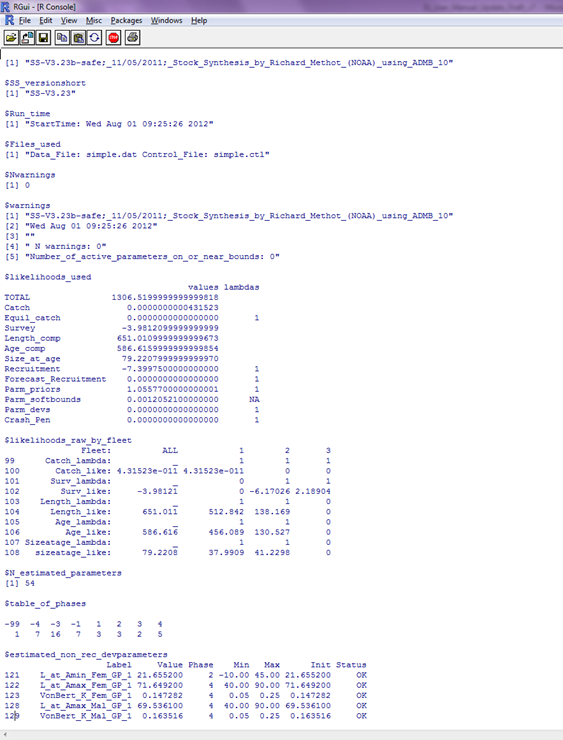
\includegraphics{r4ss_output}
\end{center}

\pagebreak
Example of the plots created using the SS\_plots function:
\begin{center}
	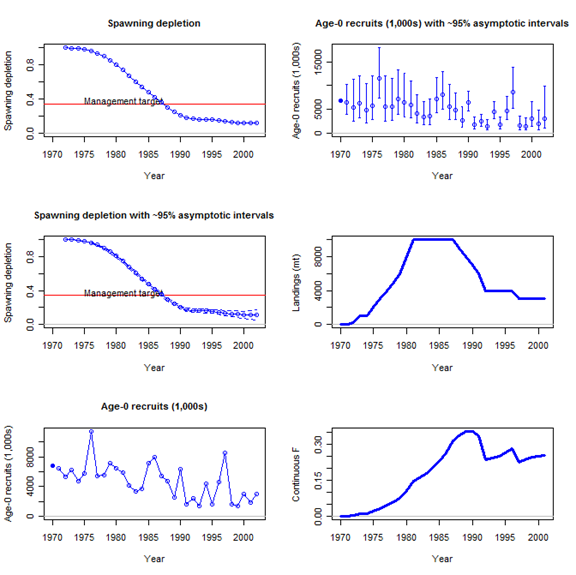
\includegraphics{r4ss_plots}
\end{center}

\pagebreak
The functions included in r4ss ranging from general use to functions developed for specific model applications:
\begin{center}
	\begin{longtable}{p{4.5cm} p{10.52cm}}
		Core Functions & \\
		\hline
		SS\_output & A function to create a list object for the output from Stock Synthesis\\
		SS\_plots  & Plot many quantities related to output from Stock Synthesis\\
		\hline
		\\
		\multicolumn{2}{l}{Plot functions called by SS\_plots} \\
		\hline
		SSplotBiology & Plot biology related quantities \\
		SSplotCatch   & Plot catch related quantities \\
		SSplotCohorts & Plot cumulative catch by cohort \\
		SSplotComps   & Plot composition data and fits \\
		SSplotData    & Timeline of presence/absence data by type, year, and fleet \\
		SSplotDiscard & Plot fit to discard fraction \\
		SSplotIndices & Plot indices of abundance and associated quantities \\
		SSplotMnwt    & Plot mean weight data and fits \\
		SSplotMovementMap & Show movement rates on a map \\
		SSplotMovementRates & Show movement rates on a map \\
		SSplotNumbers & Plot numbers-at-age related data and fits \\
		SSplotRecdevs & Plot recruitment deviations \\
		SSplotRecdist & Plot of recruitment distribution among areas and seasons \\
		SSplotSelex   & Plot selectivity \\
		SSplotSexRatio & Plot sex ratios \\
		SSplotSummaryF & Plot time series summary of F (or harvest rate) \\
		SSplotSpawnrecruit & Plot spawner-recruit curve \\
		SSplotSPR     & Plot SPR quantities \\
		SSplotTags    & Plot tagging data and fits \\
		SSplotTimeseries & Plot time series data \\
		SSplotYield   & Plot yield and surplus production \\
		SS\_html       & Create HTML files to view figures in browser \\
		SS\_fitbiasramp & Estimate bias adjustment for recruitment deviates \\
		\hline
		\\
		\multicolumn{2}{l}{Model Comparisons and other diagnostics} \\
		\hline
		SSplotPars    & Plot distributions of priors, posteriors, and estimates \\
		SSplotProfile & Plot likelihood profile results \\
		PinerPlot     & Plot fleet-specific contributions to likelihood profile \\
		SSplotRetroRecruits & Make retrospective patter of recruitment estimates (a.k.a squid plot) as seen in Pacific hake assessments \\
		\hline
		\\
		\multicolumn{2}{l}{Functions related to MCMC diagnostics}\\
		\hline 
		mcmc\_nuisance & Summarize nuisance MCMC output \\
		mcmc\_out      & Summarize, analyze, and plot key MCMC output \\
		SSgetMCMC      & Read MCMC output \\
		SSplotMCMC\_ExtraSelex & Plot uncertainty around chosen selectivity ogive from MCMC \\
		\hline
		\\
		\multicolumn{2}{l}{Interactive tools for exploring functional forms} \\
		\hline
		movepars      & Explore movement parameterization \\
		selfit        & A function to visualize parameterization of double normal and double logistic selectivity in SS \\
		selfit\_spline & Visualize parameterization of cubic spline selectivity in SS \\
		sel\_line     & A function for drawing selectivity curves \\
		\hline
		\\
		\multicolumn{2}{l}{File manipulation for inputs}\\
		\hline
		SS\_readdat   & Read data file \\
		SS\_readforecast & Read forecast file \\
		SS\_readstarter  & Read starter file \\
		SS\_writedat  & Write data file \\
		SS\_writeforecast & Write forecast file \\
		SS\_writestarter  & Write starter file \\
		SS\_makedatlist   & Make a list for SS data \\
		SS\_parlines      & Get parameter lines from SS control file \\
		SS\_changepars    & Change parameters in the control file \\
		SSmakeMmatrix     & Create inputs for entering a matrix of natural mortality by age and year \\
		SS\_profile       & Run a likelihood profile in SS (incomplete) \\
		NegLogInt\_Fn     & Calculated variances of time-varying parameters using SS implementation of the Laplace Approximation \\
		\hline
		\\
		\multicolumn{2}{l}{File manipulations for outputs}\\
		\hline
		SS\_recdevs      & Insert a vector of recruitment deviations into the control file \\
		SS\_splitdat     & Split apart bootstrap data to make input file \\
		\hline
		\\
		\multicolumn{2}{l}{Minor plotting functions}\\
		\hline
		bubble3          & Create a bubble plot \\
		make\_multifig   & Create multi-figure plots \\
		Make\_multifig\_sexratio & Create multi-figure plots of sex ratios \\
		plotCI           & Plot points with confidence intervals \\
		rich\_colors\_short & Make a vector of colors \\
		stackpoly        & Plot stacked polygons \\
		mountains        & Make shaded polygons with a mountain-like appearance \\
		\hline
		\\
		\multicolumn{2}{l}{Really specialized functions} \\
		\hline
		DoProjectPlots   & Make plots from Rebuilder program \\
		IOTCmove         & Make a map of movement for a 5-area Indian Ocean model \\
		SSFishGraph      & A function for converting SS output to the format used by FishGraph \\
		TSCplot          & Create a plot for the TSC report \\
		\hline
	\end{longtable}
\end{center}
	
		%========= Section 14: Special Set-ups
		\section{Special Set-ups}

\subsection{Continuous seasonal recruitment}
It is awkward in SS to set up a seasonal model such that recruitment can occur with similar and independent probability in any season of any year.  Consequently, some users have attempted to setup SS so that each quarter appears as a year.  They have set up all the data and parameters to treat quarters as if they were years (i.e. each still has a duration of 1.0 time step).  This can work, but requires that all rate parameters be re-scaled to be correct for the quarters being treated as years.

Another option is available.  If there is one season per year and the season duration is set to 3 (rather than the normal 12), then the season duration is calculated to be 3/12 or 0.25.  This means that the rate parameters can stay in their normal per year scaling and this shorter season duration makes the necessary adjustments internally.  Some other adjustments to make when doing quarters as years include:

\begin{itemize}
	\item re-index all "year seas" inputs to be in terms of quarter-year because all are now season 1; increase endyr value in sync with this
	\item increase max age because age is now in quarters
	\item in the age error definitions, increase the number of entries in accord with new max age
	\item in the age error definitions, recode so that each quarter-age gets assigned to the correct agebin;  This is because the age data are still in terms of agebins; i.e. the first 4 entries for quarter-ages 1 through 4 will all be assigned to agebin 1.5; the next four to agebin 2.5;  you cannot accomplish the same result by editing the age bin values because the stddev of ageing error is in terms of agebin
	\item in the control file, multiple the natM age breakpoints  and growth AFIX values by 1/seasdur
	\item decrease the R0 parameter starting value because it is now the average number of recruitments per qtryear
	\item edit the rec\_dev start and endyrs to be in terms of qtryear
	\item edit any age selectivity parameters that refer to age to now refer to qtrage
	\item if there needs to be some degree of seasonality to recruitment or some parameter, then you could create a cyclic pattern in the environmental input and make recruitment or some other parameter a function of this cyclic pattern
\end{itemize}
	
A good test showing comparability of the 3 approaches to setting up a quarterly model should be done.


		%========= Section 15: Change Log
		\section{Change Log}

This section has been removed from the user manual.  Information on changes to SS is now recorded in the spreadsheet database, SS\_Changes.xlsx.  Fields include date, version number, category (e.g. growth, selectivity), type (e.g. new, clarify, fix).  Occasional model tips will be added with the type=”Tip”.	
		%========= Section 16: Appendix A: Recruitment 
		\section{Appendix A: Recruitment Variability and Bias \\ Correction }


Recruitments in SS are defined as lognormal deviates around a log-bias adjusted spawner- recruitment curve.  The magnitude of the log-bias adjustment is calculated from the level of $\sigma_R$ , which is the standard deviation of the recruitment deviations (in log-space).  There are 5 segments of the time series in which to consider the effect of the log-bias adjustment: virgin; initial equilibrium; early data-poor period; data-rich period; very-recent/forecast. The choice of break points between these segments need not correspond directly with the settings for the bias adjustment, although some alignment might be desired. Methot and Taylor (2011) provide more detailed discussion of the bias adjustment than what is provided below but do not address the separation of time periods into separate segments. The approach is illustrated with figures associated with a recent assessment for darkblotched rockfish (Gertseva and Thorson, 2013).

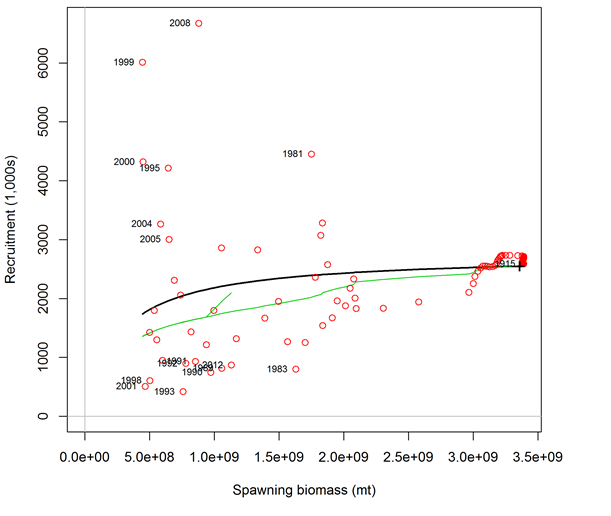
\includegraphics{appendixA_recruits}\\
\figurename{ A.1. Spawner-recruitment relationship for darkblotched rockfish (Gertseva and Thorson, 2013). Red points represent estimated recruitments, the solid black line is the stock-recruit relationship and the green line represents the adjustment to this relationship after adjustment to account for the lognormal distribution associated with each year. The “+” symbol labeled 1915 near the right side represents both the virgin and initial equilibrium of the model. The numerous red points close to the initial conditions correspond to the early years of the model with low harvest rates.}

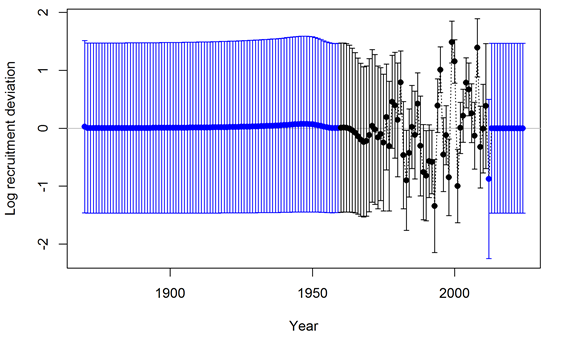
\includegraphics{appendixA_logdevs}\\
\figurename{ A.2. Timeseries of log recruitment deviations for darkblotched rockfish with 95\% uncertainty intervals. The start year of the model is 1915, but recruitment deviations are estimates starting in 1870. The 45 deviation estimates for 1870–1914 inform the age structure used in the start year. The black color for the years 1960–2011 indicates the “main” recruitment deviation vector, while the blue color for the years 1870–1959 and 2012–2024 indicates the “early” and “late/forecast” recruitment deviation vectors, respectively. }

\begin{description}
	\item[Virgin]\hfil\\
	The R0 level of recruitment is a parameter of the spawner-recruitment curve.  This recruitment and the corresponding spawning biomass, S0, are expected to represent the long-term arithmetic mean.
	\item[Initial Equilibrium]\hfil\\
	The level of recruitment is typically maintained at the R0 level even though the initial equilibrium catch will reduce the spawning biomass below the virgin level.  If steepness is moderately low or the initial F is high, then the lack of response in recruitment level may appear paradoxical.  The logic is that building in the spawner-recruitment response to initial F would significantly complicate the calculations and would imply that the initial equilibrium catch level had been going on for multiple generations.  If the lack of response is considered to be problematic in a particular application, then start the model at an earlier year and with a lower initial equilibrium catch so that the dynamics of the spawner-recruitment response get captured in the early period, rather than getting lost in the initial equilibrium.
	\item[Early data-poor period]\hfil\\
	This is the early part of the time series where the only data typically are landed catch.  There are no data to inform the model about the specific year-to-year fluctuations in recruitment, although the ending years of this period will begin to be influenced by the data.  The “early time period” is not a formal concept. 	It is up to the user to decide whether to start estimating recruitment deviations beginning with the first year of the model, or to delay such estimation until the data become more informative. Modeling recruitment deviations in this period may lead to a more realistic portrayal of the uncertainty in depletion, but can also lead to spurious patterns in estimated recruitments that may be driven by the fit to index data or other sources that would not be expected to have accurate information on recruitment.
	\begin{itemize}
		\item Option A: Do not estimate recruitment deviations during this early period.  During years prior to the first year of recruitment deviations, the model will set the recruitment equal to the level of the spawner-recruitment curve.  Thus, it is a mean-based level of recruitment.  Because these annual parameters are fixed to the level of the spawner-recruitment curve, they have no additional uncertainty and make no contribution to the variance of the model. This approach may produce relatively large, or small, magnitude deviations at the very beginning of the subsequent period, as the model “catches up” to any slight signal that could not be captured through estimated deviations in the early data-poor period.  There may be some effect on the estimate of R0 as a result of lack of model flexibility in balancing early period removals with signal in the early portion of the data-rich period.  
		\item Option B: Estimate recruitment deviations for all the early years.  Each of these recruitment deviations is now a dev parameter so will have a variance that contributes to the total model variance.  The estimated standard deviation of each of these dev parameters should be similar to $\sigma_R$ because $\sigma_R$ is the only constraint on these parameters (however, the last few in the sequence will begin to feel the effect of the data so may have lower standard deviations). 		
	\end{itemize}
	\item[Data-rich period]\hfil\\
	Here the data inform the model on the year-to-year level of recruitment.  These fluctuations in recruitment are assumed to have a lognormal distribution around the log-bias adjusted spawner-recruitment curve.  The level of $\sigma_R$ input to the model should match this level of fluctuation to a reasonable degree.  Because the recruitments are lognormal, they produce a mean biomass level that is comparable to the virgin biomass and thus the depletion level can be calculated without bias.  However, if the early period has recruitment deviations estimated by MPD, then the depletion levels during the early part of the data-rich period may have some lingering effect of negative bias during the early time period. The level of $\sigma_R$ should be at least as large as the level of variability in these estimated recruitments.  If too high a level of $\sigma_R$ is used, then a bias can occur in the estimate of spawner-recruitment steepness, which determines the trend in recruitment.  This occurs when the early recruitments are taken directly from the spawner-recruitment curve, so are mean unbiased, then the later recruitments are estimated as deviations from the log-bias adjusted curve.  If $\sigma_R$ is too large, then the bias-adjustment is too large, and the model may compensate by increasing steepness to keep the mean level of recent recruitments at the correct level.
	\item[Recent Years/Forecast]\hfil\\
	Here the situation is very similar to the early time period in that there are no data to inform the model about the year-to-year pattern in recruitment fluctuations so all devs will be pulled to a zero level in the MPD.  The structure of SS creates no sharp dividing line between the estimation period and the forecast period.  In many cases one or more recruitments at the end of the time series will lack appreciable signal in the data and should therefore be treated as forecast recruit deviations.  To the degree that some variability is observed in these recruitments, partial or full bias correction may be desirable for these devs separate from the purely forecast devs, there is therefore an additional control for the level of bias correction applied to forecast deviations occurring prior to endyear+1.
\end{description}

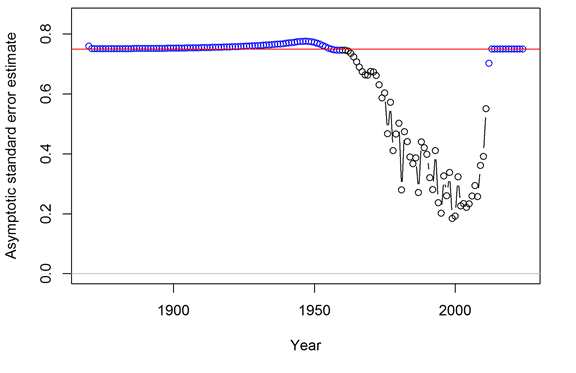
\includegraphics{appendixA_asymerror}\\
\figurename{ A.3. Timeseries of standard error estimates for the log recruitment deviations for darkblotched rockfish with 95\% uncertainty intervals. As in Figure A.2, the black color indicates the main recruitment period. This period with lower standard error is associated with higher variability among deviations (Figure A.2). The red line at 0.75 indicates the  $\sigma_R$ value in this model.}

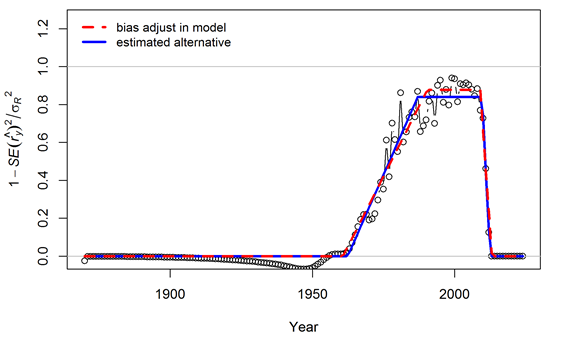
\includegraphics{appendixA_biasadj}\\
\figurename{ A.4. Transformation of the standard error estimates (shown in Figure A.3) for darkblotched rockfish following the approach suggested by Methot and Taylor (2011). These values were used to set the 5 values controlling the degree of bias adjustment (as a fraction of  $\sigma_R/2$) to account for differences in the mean and median of the lognormal distribution from which the recruitment deviations are drawn. The red line indicates a bias adjustment of 0 up to the  1960.75, ramping up to a maximum adjustment level of 0.877 for the period 1990.4–2008.98,and reducing back to 0 starting in 2013.08. Note that these values controlling the bias adjustment need not be integer year values. Also the break points in the bias adjustment function need not match the break points between early, main, and late/forecast recruitment deviation vectors (indicated by blue and black colors in Figures A.2 and A.3). The blue line indicates a functional form that minimizes the sum of squared differences between the bias adjustment function and the transformed standard error values. The subtle differences between red and blue lines are unlikely to have any appreciable effect on the model results.}

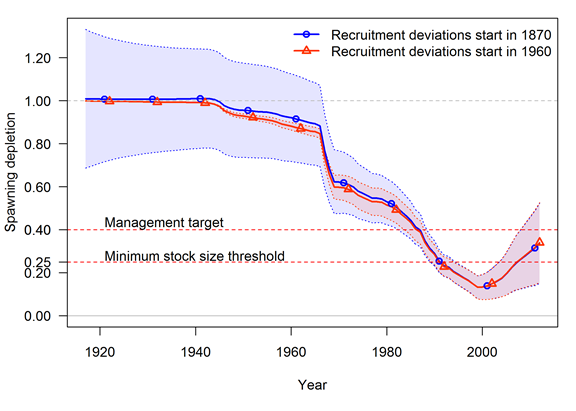
\includegraphics{appendixA_depl}\\
\figurename{ A.5. Comparison of timeseries of spawning depletion for darkblotched rockfish models with early recruitment deviations (starting in 1870) and without early deviations (only main recruitment deviations starting in 1960). The point estimates are similar, but the 95\% uncertainty intervals are substantially different. With no recruitment deviations for the early period, the estimates of spawning depletion in the early years are very precise and uncertainty increases as the stock moves into the data rich period. In contrast, the addition of the early recruitment deviations results in a large uncertainty in spawning depletion for the early years and an increase in precision as the stock moves into the data rich period. In this application, the uncertainty associated with the recent years is independent of the assumptions about early recruitments.}

\subsection{Issues with Including Environmental Effects}
The expected level of recruitment is a function of spawning biomass, an environmental time series, and a log-bias adjustment.
\begin{equation}
	E(Recruitment) = f(SpBio) * exp(\beta*envdata) * exp(-0.5*\sigma_R^2)
\end{equation}
$\sigma_R$ is the variability of the deviations, so it is in addition to the variance “created” by the environmental effect.  So, as more of the total recruitment variability is explained by the environmental effect, the residual $\sigma_R$ should be decreased.  The model does not do this automatically.

The environmental effect is inherently lognormal.  So when an environmental effect is included in the model, the arithmetic mean recruitment level will be increased above the level predicted by f(SpBio) alone.  The consequences of this have not yet been thoroughly investigated, but there probably should be another bias correction based on the variability of the environmental data as scaled by the estimated linkage parameter, $\beta$.  It is also problematic that the environmental effect time series used as input is assumed to be measured without error.

The preferred approach to including environmental effects on recruitment is not to use the environmental effect in the direct calculation of the expected level of recruitment.  Instead, the environmental data would be used as if it was a survey observation of the recruitment deviation.  This approach is similar to using the environmental index as if it was a survey of age 0 recruitment abundance because by focusing on the fit to the deviations it removes the effect of SpBio on recruitment.  In this alternative, the $\sigma_R$ would not be changed by the environmental data; instead the environmental data would be used to explain some of the total variability represented by $\sigma_R$.  This approach may also allow greater uncertainty in forecasts, as the variability in projected recruitments would reflect both the uncertainty in the environmental observations themselves and the model fit to these observations.

\subsection{Initial Age Composition}
If the first year with recruitment deviations is set less than the start year of the model, then these early deviations will modify the initial age composition.  The amount of information on historical recruitment variability certainly will degrade as the model attempts to estimate deviations for older age groups in the initial equilibrium.  So the degree of bias correction is reduced linearly in proportion to age so that the correction disappears when maximum age is reached.  The initial age composition approach normally produces a result that is indistinguishable from a configuration that starts earlier in the time series and estimates a longer time series of recruitments.  However, because the initial equilibrium is calculated from a recruitment level unaffected by spawner-recruitment steepness and initial age composition adjustments are applied after the initial equilibrium is calculated, it is possible that the initial age composition approach will produce a slightly different result than if the time series was started earlier and the deviations were being applied to the recruitment levels predicted from the spawner-recruitment curve. 
	
		%========= Section 17: Appendix B: Forecast Module
		\hypertarget{appendB}{}
\section{Appendix B: Forecast Module}


\subsection{Introduction}
Version 3.20 of Stock Synthesis (SS) introduced substantial upgrades to the benchmark and forecast module.  The general intent was to make the forecast outputs more consistent with the requirement to set catch limits that have a known probability of exceeding the overfishing limit.  In addition, this upgrade addressed several inadequacies with the previous module, including:

\begin{itemize}
	\item The average selectivity and relative F was the same for the benchmark and the forecast calculations;
	\item The biology-at-age in endyr+1 was used as the biology for the benchmark, but biology–at-age propagated forward in the forecast if there was time-varying growth;
	\item The forecast module had a kluge approach to calculation of OFL conditioned on previously catching ABC;
	\item The forecast module implementation of catch caps was incomplete and applied some caps on a seasonally, rather than the more logical annual basis;
	\item The Fmult scalar for fishing intensity presented a confusing concept for many users;
	\item No provision for specification of catch allocation among fleets;
	\item The forecast allowed for a blend of fixed input catches and catches calculated from target F; this is not optimal for calculation of the variance of F conditioned on a catch policy that sets ACLs.
\end{itemize}

The V3.20 module addressed these issues by:
\begin{itemize}
	\item Providing for unique specification of a range of years from which to calculate average selectivity for benchmark, average selectivity for forecast, relative F for benchmark, and relative F for forecast;
	\item Create a new specification for the range of years over which to average size-at-age and fecundity-at-age for the benchmark calculation.  In a setup with time-varying growth, it may make sense to do this over the entire range of years in the time series.  Note that some additional quantities still use their endyr values, notably the migration rates and the allocation of recruitments among areas.  This will be addressed shortly;
	\item Create a multiple pass approach that rectifies the OFL calculation;
	\item Improve the specification of catch caps and implement specification of catch allocations so that there can be an annual cap for each fleet, an annual cap for each area, and an annual allocation among groups of fleets (e.g. all recreational fleets vs. all commercial fleets);
	\item Introduce capability to have implementation error in the forecast catch (single value applied to all fleets in all seasons of the year).
\end{itemize}

\subsection{Multiple Pass Forecast}
The most complicated aspect of the changes is with regard to the multiple pass aspect of the forecast.  This multiple pass approach is needed to calculate both OFL and ABC in a single model run.  More importantly, the multiple passes are needed in order to mimic the actual sequence of assessment-management action – catch over a multi-year period.  The first pass calculates OFL based on catching OFL each year, so presents the absolute maximum upper limit to catches.  The second pass forecasts a catch based on a harvest policy, then applies catch caps and allocations, then updates the F’s to match these catches.  In the third pass, stochastic recruitment and catch implementation error are implemented and SS calculates the F that would be needed in order to catch the adjusted catch amount previously calculated in the second pass.  With this approach, SS is able to produce improved estimates of the probability that F would exceed the overfishing F.  In effect it is the complement of the P* approach.  Rather than the P* approach that calculates the stream of annual catches that would have an annual probability of F>Flimit, SS calculates the expected time series of P* that would result from a specified harvest policy implemented as a buffer between Ftarget and Flimit.

The sequence of multiple forecast passes is as follows:
\begin{enumerate}
	\item Pass 1 (a.k.a. Fcast\_Loop1)
	\begin{enumerate}
		\item Loop Years
		\begin{enumerate}
			\item SubLoop (a.k.a. ABC\_Loop) = 1
			\begin{enumerate}
				\item R=f(SSB) with no deviations
				\item F=Flimit
				\item Fixed input catch amounts ignored
				\item No catch adjustments (caps and allocations)
				\item No implementation error
				\item Result: OFL conditioned on catching OFL each year
			\end{enumerate}
		\end{enumerate}
	\end{enumerate}
	\item Pass 2
	\begin{enumerate}
		\item Loop Years
		\begin{enumerate}
			\item SubLoop = 1
			\begin{enumerate}
				\item R=f(SSB) with no deviations
				\item F=Flimit
				\item Fixed input catch amounts ignored
				\item No catch adjustments (caps and allocations)
				\item No implementation error
				\item Result: OFL conditioned on catching ABC previous year. Stored in std\_vector.
			\end{enumerate}
			\item SubLoop = 2
			\begin{enumerate}
				\item R=f(SSB) with no deviations
				\item F=Ftarget to get catc for each fleet in each season
				\item Fixed input catch amounts replace catch from step 2
				\item Catch adjustments (caps and allocations) applied on annual basis (after looping through seasons and and areas within this year). These adjustments utilize the logistic joiner approach common in SS so the overall results remain completely differentiable.
				\item No implementation error
				\item Result: ABC as adjusted for caps and allocations
			\end{enumerate}
			\item SubLoop = 3
			\begin{enumerate}
				\item R=f(SSB) with no deviations
				\item Catches from Pass 2 multiplied by the random term for implementation error
				\item F=adjusted to match the catch*error while taking into account the random recruitments.  This is most easily visualized in a MCMC context where the recruitment deviation and the implementation error deviations take on non-zero values in each instance.  In MLE, because the forecast recruitments and implementation error are estimated parameters with variance, their variance still propagates to the derived quantities in the forecast.
				\item Result:  Values for F, SSB, Recruitment, Catch are stored in std-vectors
				\begin{itemize}
					\item In addition, the ratios F/Flimit and SSB/SSBlimit or SSB/SSBtarget are also stored in std\_vectors.
					\item Estimated variance in these ratios allows calculation of annual probability that F>Flimit or B<Blimit.  This is essentially the realized P* conditioned on the specified harvest policy.
				\end{itemize}
			\end{enumerate}
		\end{enumerate}
	\end{enumerate}
\end{enumerate}

\subsection{Example Effects on Correlations}
An example that illustrates the above process was conducted.  The situation was a low M, late-maturing species, so changes are not dramatic.  The example conducted a 10 year forecast and examined correlations with derived quantities in the last year of the forecast.  This was done once with the full set of 3 passes as described above, and again with only 2 passes and stochastic recruitment occurring in pass 2, rather than 3.  This alternative setup is more similar to forecasts done using previous model versions.

\begin{center}
	\begin{longtable}{p{0.4cm} p{2.75cm} p{3cm} p{1cm} p{0.4cm} p{2.75cm} p{2cm} p{1cm}}
		\hline
		 & \multicolumn{3}{l}{2 Forecast Passes with F from} & & \multicolumn{3}{l}{2 Forecast Passes with catch from}\\
		 & \multicolumn{3}{l}{ABC and random recruitment} & & \multicolumn{3}{l}{target F and equilibrium recruitment}\\
		\hline
		 & Factor X & Factor Y & Corr &  & Factor X & Factor Y & Corr \\
		 \hline
		 A1 & F 2011 & RecrDev 2002 & -0.126 & A2 & F 2011 & RecrDev 2002 & 0.090 \\
		 B1 & F 2011 & Recr 2002    &  0.312 & B2 & F 2011 & Recr    2002 & 0.518 \\
		 C1 & ForeCatch 2011 & RecrDev 2002 & 0.000 & C2 & ForeCatch 2011 & RecrDev 2002 & 0.129 \\
		 D1 & ForeCatch 2011 & Recr 2002    & 0.455 & D2 & Forecatch 2011 & Recr 2002    & 0.555 \\
		 \hline		
	\end{longtable}
\end{center}

Correlation A2 shows a small positive correlation between the recruitment deviation in 2002 and the F in 2011.  This is probably due to the fact that a positive deviation in recruitment in 2002 will reduce the chances that the biomass in 2011 will be below the inflection point in the control rule.  This occurs because in calculating catch from F, the model effectively “knows” the future recruitments.  I predict that this B1 correlation would be near zero if there was no inflection in the control rule.
Correlation A1 shows this turning into a negative correlation.  This is because the future catches are first calculated from equilibrium recruitment, then when random recruitments are implemented, a positive recruitment deviation will cause a negative deviation in the F needed to catch that now “fixed” amount of future catch.

Correlations B1 and B2 are in terms of absolute recruitment, not recruitment deviation.  Now overall model conditions that cause a higher absolute recruitment level will also result in a higher forecast level.  No surprise there, and the correlation is stronger when variance is based on catch is calculated from F (B2).

Correlation C2 shows a positive correlation between recruitment deviation in 2002 and forecast catch in 2011.  However, correlation C1 is 0.0 because the forecast catch in 2011 is set based on equilibrium recruitment and is not influenced by the recruitment deviations.

\subsection{Future Work}
\begin{itemize}
	\item More testing with high M, rapid turnover conditions
	\item Testing without inflection in control rule
	\item Consider separating implementation error into a pass \#4 so results will more clearly show effect of assessment uncertainty separate from implementation uncertainty
	\item 	Consider adding a random “assessment” error which essentially is a random variable that scales population abundance before passing into the forecast stage.  Complication is figuring out how to link it to the correlated error in the benchmark quantities
	\item Because all of these calculations occur only in the sdphase or the mceval phase, it would be feasible for mceval calls to add an additional pass that is implemented many times and in which random forecast recruitment draws are made.
	\item Factors like selectivity and fleet relative F levels are calculated as an average of these values during the time series.  This is internally consistent if these factors do not vary during the time series (although clearly this is a stiff model that will underestimate process variance).  However, if these factors do vary over time, then the average used for the forecast will under-represent the variance.  A better approach would be to set up the parameters of selectivity as a random process that extends throughout the forecast period, and to update estimated selectivity in each year of the forecast based upon the random realization of these parameters.
\end{itemize}

	
	
		%========= Section 18: Appendix B: Forecast Module
		\section{Appendix C: Code Examples}

\subsection{Ageing Error Estimation}
\hypertarget{AgeingError}{}
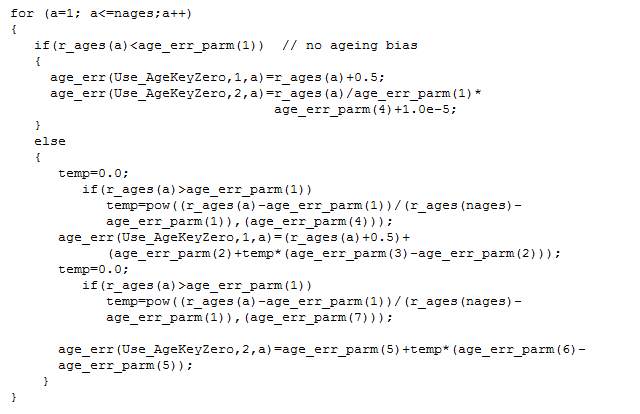
\includegraphics{age_error}
The 7 parameters are:

\begin{itemize}
	\item age at which the estimated pattern begins (just linear below this age).  This is “start age”
	\item bias at start age (as additive offset from unbiased age’)
	\item bias at maxage (as additive offset from unbiased age’)
	\item power fxn coefficient for interpolating between those 2 values (value of 0.0 produces linear interpolation in the bias)
	\item stdev at age
	\item stdev at max age
	\item power fxn coefficient for interpolating between those 2 values
\end{itemize}


\subsection{Survival Based SRR Code}
\hypertarget{AppendixC}{Code} for the survival based recruitment is shown below:\\
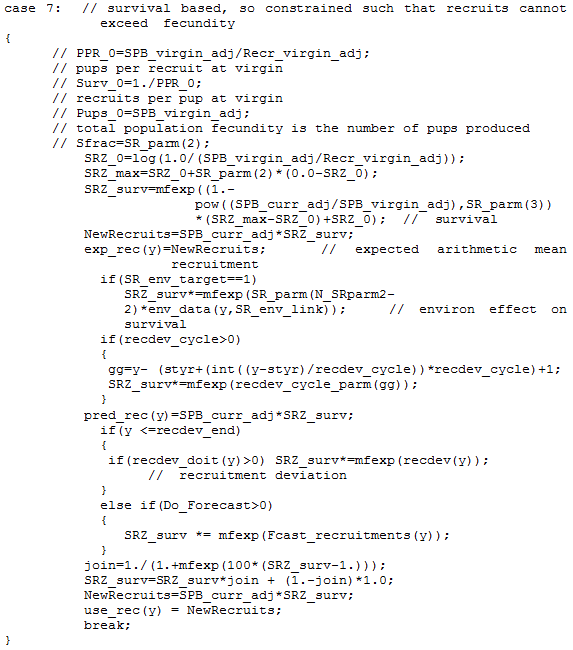
\includegraphics{survival_code}

\subsection{Random Walk Selectivity: Pattern 17}
\hypertarget{RandWalkSelex}{}
	\begin{center}
		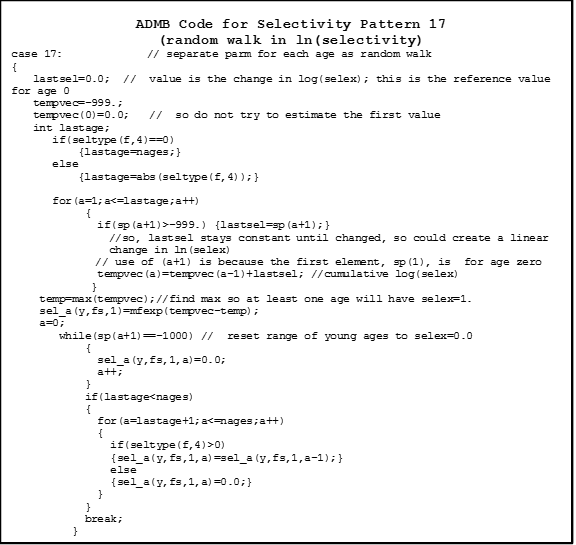
\includegraphics{Selex17_RandomWalk}
		\end{center}

\subsection{Cubic Spline Selectivity}
\hypertarget{CubicSpline}{}
	\begin{center}
		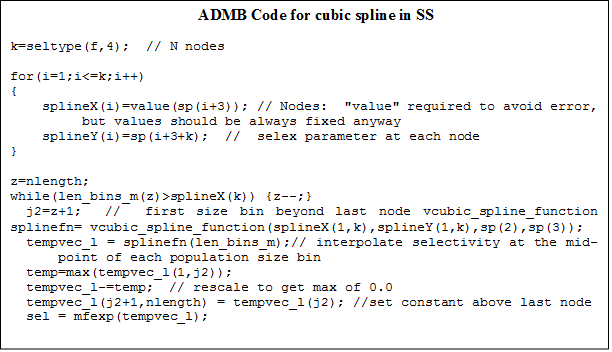
\includegraphics{CubicSplineCode}
	\end{center}	
		%========= Section 19: Input File
		\section{Appendix D: Example Files}

\subsection{Starter File}

\subsection{Run Number}

\subsection{Profile Values}

\subsection{Forecast File}

\subsection{Control File}

\subsection{Data File}
		%========= Section 19: Input File
		\begin{landscape}

\section{Appendix E: Example Model Files}


\subsection{starter.ss}
\scriptsize{
\begin{verbatim}
	#V3.30a
	#C starter comment here
	simple_disc.dat
	simple_lendisc.ctl
	0 # 0=use init values in control file; 1=use ss3.par
	1 # run display detail (0,1,2)
	1 # detailed age-structured reports in REPORT.SSO (0,1) 
	0 # write detailed checkup.sso file (0,1) 
	1 # write to cumreport.sso (0=no,1=like&timeseries; 2=add survey fits)
	1 # Include prior_like for non-estimated parameters (0,1) 
	1 # Use Soft Boundaries to aid convergence (0,1) (recommended)
	3 # Number of datafiles to produce: 1st is input, 2nd is estimates, 3rd and higher are bootstrap
	100 # Turn off estimation for parameters entering after this phase
	0 # MCeval burn interval
	1 # MCeval thin interval
	0 # jitter initial parm value by this fraction
	1969 # min yr for sdreport outputs (-1 for styr)
	2004 # max yr for sdreport outputs (-1 for endyr; -2 for endyr+Nforecastyrs
	0 # N individual STD years 
	#vector of year values 	
	0.0001 # final convergence criteria (e.g. 1.0e-04) 
	0 # retrospective year relative to end year (e.g. -4)
	1 # min age for calc of summary biomass
	1 # Depletion basis:  denom is: 0=skip; 1=rel X*B0; 2=rel X*Bmsy; 3=rel X*B_styr
	0.4 # Fraction (X) for Depletion denominator (e.g. 0.4)
	1 # SPR_report_basis:  0=skip; 1=(1-SPR)/(1-SPR_tgt); 2=(1-SPR)/(1-SPR_MSY); 3=(1-SPR)/(1-SPR_Btarget);
	# 4=rawSPR
	4 # F_report_units: 0=skip; 1=exploitation(Bio); 2=exploitation(Num); 3=sum(Frates); 4=true F for range 
	# of ages
	20 23 #_min and max age over which average F will be calculated
	1 # F_std_basis: 0=raw_F_report; 1=F/Fspr; 2=F/Fmsy ; 3=F/Fbtgt
	0 # ALK tolerance (example 0.0001)
	3.3 # check value for end of file and for version control
\end{verbatim}
}


\subsection{forecast.ss}
\scriptsize{
\begin{verbatim}
	#V3.30a
	1 # Benchmarks: 0=skip; 1=calc F_spr,F_btgt,F_msy 
	2 # MSY: 1= set to F(SPR); 2=calc F(MSY); 3=set to F(Btgt); 4=set to F(endyr) 
	0.4 # SPR target (e.g. 0.40)
	0.342 # Biomass target (e.g. 0.40)
	#_Bmark_years: beg_bio, end_bio, beg_selex, end_selex, beg_relF, end_relF (enter actual year, or values of
	# 0 or -integer to be rel. endyr)
	0 0 0 0 0 0
	#  2001 2001 2001 2001 2001 2001 # after processing 
	1 #Bmark_relF_Basis: 1 = use year range; 2 = set relF same as forecast below
	#
	1 # Forecast: 0=none; 1=F(SPR); 2=F(MSY) 3=F(Btgt); 4=Ave F (uses first-last relF yrs); 5=input annual F
	# scalar
	3 # N forecast years 
	0.2 # F scalar (only used for Do_Forecast==5)
	#_Fcast_years:  beg_selex, end_selex, beg_relF, end_relF  (enter actual year, or values of 0 or -integer to
	# be rel. endyr)
	0 0 -10 0
	#  2001 2001 1991 2001 # after processing 
	1 # Control rule method (1=catch=f(SSB) west coast; 2=F=f(SSB) ) 
	0.4 # Control rule Biomass level for constant F (as frac of Bzero, e.g. 0.40); (Must be > the no F level
	# below) 
	0.1 # Control rule Biomass level for no F (as frac of Bzero, e.g. 0.10) 
	0.75 # Control rule target as fraction of Flimit (e.g. 0.75) 
	3 #_N forecast loops (1=OFL only; 2=ABC; 3=get F from forecast ABC catch with allocations applied)
	3 #_First forecast loop with stochastic recruitment
	0 #_Forecast loop control #3 (reserved for future bells&whistles) 
	0 #_Forecast loop control #4 (reserved for future bells&whistles) 
	0 #_Forecast loop control #5 (reserved for future bells&whistles) 
	2010  #FirstYear for caps and allocations (should be after years with fixed inputs) 
	0 # stddev of log(realized catch/target catch) in forecast (set value>0.0 to cause active impl_error)
	0 # Do West Coast gfish rebuilder output (0/1) 
	1999 # Rebuilder:  first year catch could have been set to zero (Ydecl)(-1 to set to 1999)
	2002 # Rebuilder:  year for current age structure (Yinit) (-1 to set to endyear+1)
	1 # fleet relative F:  1=use first-last alloc year; 2=read seas(row) x fleet(col) below
	# Note that fleet allocation is used directly as average F if Do_Forecast=4 
	2 # basis for fcast catch tuning and for fcast catch caps and allocation  (2=deadbio; 3=retainbio; 
	# 5=deadnum; 6=retainnum)
	# Conditional input if relative F choice = 2
	# Fleet relative F:  rows are seasons, columns are fleets
	#_Fleet:  FISHERY1 SURVEY1 SURVEY2
	#  1 0 0
	# enter list of fleet number and max for fleets with max annual catch; terminate with fleet=-9999
	-9999 -1
	# enter list of area ID and max annual catch; terminate with area=-9999
	-9999 -1
	# enter list of fleet number and allocation group assignment, if any; terminate with fleet=-9999
	1 1
	-9999 -1
	#_if N allocation groups >0, list year, allocation fraction for each group 
	# list sequentially because read values fill to end of N forecast
	# terminate with -9999 in year field 
	2002  1
	-9999  1 
	-1 # basis for input Fcast catch: -1=read basis with each obs; 2=dead catch; 3=retained catch; 99=input
	# Hrate(F)
	#enter list of Fcast catches; terminate with line having year=-9999
	#_Year Seas Fleet Catch(or_F) Basis 
	2003 1 1 300 2
	2004 1 1 300 2
	-9999 1 1 0  2 
	#
	999 # verify end of input 
\end{verbatim}
}



\subsection{data.ss}
\scriptsize{
\begin{verbatim}
	#V3.30a
	#_SS-V3.30a-safe;_03_23_2016;_Stock_Synthesis_by_Richard_Methot_(NOAA)_using_ADMB_11.1
	#_Start_time: Tue May 10 15:46:33 2016
	#_Number_of_datafiles: 3
	
	#_observed data: 
	#V3.30a
	1971 #_styr
	2001 #_endyr
	1 #_nseas
	12 #_months/season
	2 #_N_subseasons(even number, minimum is 2)
	1 #_spawn_seas
	2 #_Ngenders
	40 #_Nages=accumulator age
	1 #_N_areas
	3 #_Nfleets (including surveys)
	#_fleet_type: 1=catch fleet; 2=bycatch only fleet; 3=survey; 4=ignore 
	#_survey_timing: -1=for use of catch-at-age to override the month value associated with a datum 
	#_fleet_area:  area the fleet/survey operates in 
	#_units of catch:  1=bio; 2=num (ignored for surveys; their units read later)
	#_catch_mult: 0=no; 1=yes
	#_rows are fleets
	#_fleet_type, timing, area, units, need_catch_mult fleetname
	1 0.5 1 1 0 FISHERY1  # 1
	3 0.5 1 2 0 SURVEY1  # 2
	3 0.5 1 2 0 SURVEY2  # 3
	#_Catch data: yr, seas, fleet, catch, catch_se
	#_catch_se:  standard error of log(catch); can be overridden in control file with detailed F input
	-999 1 1 0 0.01
	1971 1 1 0 0.01
	1972 1 1 199.146 0.01
	1973 1 1 1001.51 0.01
	1974 1 1 1003.86 0.01
	1975 1 1 1985.41 0.01
	1976 1 1 3050.31 0.01
	1977 1 1 3995.8 0.01
	1978 1 1 5042.45 0.01
	1979 1 1 5962.91 0.01
	1980 1 1 7919.02 0.01
	1981 1 1 9916.32 0.01
	1982 1 1 9953.41 0.01
	1983 1 1 10013.5 0.01
	1984 1 1 9959.68 0.01
	1985 1 1 10085.9 0.01
	1986 1 1 9886.95 0.01
	1987 1 1 9975.21 0.01
	1988 1 1 9127.78 0.01
	1989 1 1 8028.19 0.01
	1990 1 1 6884.36 0.01
	1991 1 1 6051.55 0.01
	1992 1 1 3975.34 0.01
	1993 1 1 3983.8 0.01
	1994 1 1 3960.74 0.01
	1995 1 1 3968.42 0.01
	1996 1 1 4001.8 0.01
	1997 1 1 3034.03 0.01
	1998 1 1 3055.9 0.01
	1999 1 1 2991.88 0.01
	2000 1 1 3043.65 0.01
	2001 1 1 3028.14 0.01
	-9999 0 0 0 0
	#
	#_CPUE_and_surveyabundance_observations
	#_Units:  0=numbers; 1=biomass; 2=F; >=30 for special types
	#_Errtype:  -1=normal; 0=lognormal; >0=T
	#_Fleet Units Errtype
	1 1 0 # FISHERY1
	2 1 0 # SURVEY1
	3 0 0 # SURVEY2
	#_yr month fleet obs stderr
	1977 7 2 205170 0.3 #_ SURVEY1
	1980 7 2 100520 0.3 #_ SURVEY1
	1983 7 2 225658 0.3 #_ SURVEY1
	1986 7 2 112369 0.3 #_ SURVEY1
	1989 7 2 134954 0.3 #_ SURVEY1
	1992 7 2 87164.8 0.3 #_ SURVEY1
	1995 7 2 49204.9 0.3 #_ SURVEY1
	1998 7 2 85021.4 0.3 #_ SURVEY1
	2001 7 2 83672.6 0.3 #_ SURVEY1
	1990 7 3 3.57367 0.7 #_ SURVEY2
	1991 7 3 6.17539 0.7 #_ SURVEY2
	1992 7 3 15.4624 0.7 #_ SURVEY2
	1993 7 3 0.704832 0.7 #_ SURVEY2
	1994 7 3 20.2697 0.7 #_ SURVEY2
	1995 7 3 1.50754 0.7 #_ SURVEY2
	1996 7 3 2.91134 0.7 #_ SURVEY2
	1997 7 3 11.6444 0.7 #_ SURVEY2
	1998 7 3 3.14941 0.7 #_ SURVEY2
	1999 7 3 0.304886 0.7 #_ SURVEY2
	2000 7 3 3.72736 0.7 #_ SURVEY2
	2001 7 3 1.36641 0.7 #_ SURVEY2
	-9999 1 1 1 1 # terminator for survey observations 
	#
	1 #_N_fleets_with_discard
	#_discard_units (1=same_as_catchunits(bio/num); 2=fraction; 3=numbers)
	#_discard_errtype:  >0 for DF of T-dist(read CV below); 0 for normal with CV; -1 for normal with se; 
	# -2 for lognormal
	# note, only have units and errtype for fleets with discard 
	#_Fleet units errtype
	1 1 0 # FISHERY1
	#_yr month fleet obs stderr
	1995 7 1 255.678 0.2 #_ FISHERY1
	1996 7 1 322.972 0.2 #_ FISHERY1
	-9999 0 0 0.0 0.0 # terminator for discard data 
	#
	1 #_use meanbodysize_data (0/1)
	30 #_DF_for_meanbodysize_T-distribution_like
	# note:  use positive partition value for mean body wt, negative partition for mean body length 
	#_yr month fleet part obs stderr
	1995 7 1 2 2.31626 0.3 #_ FISHERY1
	1995 7 1 1 1.80019 0.3 #_ FISHERY1
	-9999 0 0 0 0 0 # terminator for mean body size data 
	#
	# set up population length bin structure (note - irrelevant if not using size data and using empirical wtatage
	2 # length bin method: 1=use databins; 2=generate from binwidth,min,max below; 3=read vector
	2 # binwidth for population size comp 
	10 # minimum size in the population (lower edge of first bin and size at age 0.00) 
	94 # maximum size in the population (lower edge of last bin) 
	1 # use length composition data (0/1)
	#_mintailcomp: upper and lower distribution for females and males separately are accumulated until 
	# exceeding this level.
	#_addtocomp:  after accumulation of tails; this value added to all bins
	#_males and females treated as combined gender below this bin number 
	#_compressbins: accumulate upper tail by this number of bins; acts simultaneous with mintailcomp; 
	# set=0 for no forced accumulation
	#_Comp_Error:  0=multinomial, 1=dirichlet
	#_Comp_Error2:  parm number  for dirichlet
	#_mintailcomp_addtocomp_combM+F_CompressBins_CompError_ParmSelect
	0 1e-007 0 0 0 0 #_fleet:1_FISHERY1
	0 1e-007 0 0 0 0 #_fleet:2_SURVEY1
	0 1e-007 0 0 0 0 #_fleet:3_SURVEY2
	# sex codes:  0=combined; 1=use female only; 2=use male only; 3=use both as joint sexxlength distribution
	# partition codes:  (0=combined; 1=discard; 2=retained
	25 #_N_LengthBins; then enter lower edge of each length bin
	26 28 30 32 34 36 38 40 42 44 46 48 50 52 54 56 58 60 62 64 68 72 76 80 90
	#_yr month fleet sex part Nsamp datavector(female-male)
	1971 7 1 3 0 125 0 0 0 0 0 0 0 0 0 6 1 3 1 3 5 2 2 5 3 6 9 1 9 0 0 0 0 0 0 0 0 0 0 4 1 0 0 3 2 3 5 3 7 7 8 14 6 6 0 0
	1972 7 1 3 0 125 0 0 0 0 0 0 0 0 0 3 1 1 0 4 3 4 6 5 8 14 8 4 6 4 0 0 0 0 0 0 0 0 0 1 1 1 2 1 0 4 5 3 5 2 6 11 8 4 0 0
	1973 7 1 3 0 125 0 0 0 0 0 0 0 0 0 0 0 0 6 1 1 4 4 3 2 14 13 9 3 0 0 0 0 0 0 0 0 0 0 0 0 0 9 2 3 4 7 3 5 2 9 9 5 5 2 0
	1974 7 1 3 0 125 0 0 0 0 0 0 0 0 0 6 0 4 0 4 2 4 3 3 4 9 6 6 9 0 0 0 0 0 0 0 0 0 2 0 2 1 3 3 2 5 7 3 7 5 5 11 5 3 1 0
	1975 7 1 3 0 125 0 0 0 0 0 0 0 0 0 0 1 1 2 1 2 3 4 3 4 13 6 7 11 0 0 0 0 0 0 0 0 0 0 0 4 2 1 0 2 6 3 5 3 8 12 10 6 5 0 0
	1976 7 1 3 0 125 0 0 0 0 0 0 0 1 1 1 0 3 0 1 1 2 6 8 5 16 7 8 6 3 0 0 0 0 0 0 0 2 2 1 0 1 2 3 0 3 2 3 6 1 6 9 8 7 0 0
	1977 7 1 3 0 125 0 0 0 0 0 0 0 1 1 0 0 1 1 3 0 5 5 2 5 8 8 5 6 3 0 0 0 0 0 0 1 0 0 2 1 4 0 4 1 6 3 8 3 4 13 9 7 5 0 0
	1978 7 1 3 0 125 0 0 0 0 0 0 2 0 1 2 1 2 0 2 3 2 2 6 8 6 6 6 4 1 0 0 0 0 0 0 0 0 6 0 0 0 2 3 1 1 4 6 3 7 22 10 5 1 0 0
	1979 7 1 3 0 125 0 0 0 0 0 0 0 0 0 0 1 3 4 5 3 3 8 6 4 9 15 4 4 2 0 0 0 0 0 0 0 0 0 4 3 3 1 2 0 2 8 2 4 2 5 8 6 3 1 0
	1980 7 1 3 0 125 0 0 0 0 0 0 0 1 0 0 0 1 0 4 1 2 1 6 4 14 8 7 4 2 0 0 0 0 0 0 0 0 0 4 2 5 3 4 3 2 1 6 2 6 13 9 7 3 0 0
	1981 7 1 3 0 125 0 0 0 0 0 0 2 0 1 0 2 0 1 2 2 4 5 8 8 6 8 5 5 0 0 0 0 0 0 0 0 0 1 0 1 3 2 2 4 4 2 4 2 6 13 10 9 3 0 0
	1982 7 1 3 0 125 0 0 0 0 0 0 0 0 2 1 2 0 1 3 3 3 4 5 4 9 14 12 0 0 0 0 0 0 0 0 0 0 2 0 2 2 2 1 6 3 5 2 5 8 13 4 4 3 0 0
	1983 7 1 3 0 125 0 0 0 0 0 0 0 0 0 0 6 1 2 2 5 6 5 4 3 10 8 10 3 0 0 0 0 0 0 0 0 0 0 0 4 2 2 3 3 2 4 3 4 2 8 11 6 6 0 0
	1984 7 1 3 0 125 0 0 0 0 0 0 0 0 1 0 0 0 2 4 4 8 6 5 5 10 10 4 8 0 0 0 0 0 0 0 0 0 1 2 0 3 2 2 2 2 7 5 3 3 12 7 3 4 0 0
	1985 7 1 3 0 125 0 0 0 0 0 0 0 0 3 1 0 3 1 2 3 6 4 8 4 6 5 2 5 1 0 0 0 0 0 0 0 0 1 1 2 2 1 3 3 6 3 8 7 2 11 8 7 6 0 0
	1986 7 1 3 0 125 0 0 0 1 0 1 1 0 1 0 1 1 3 3 3 6 7 3 5 6 9 8 8 0 0 0 0 0 0 0 1 1 0 0 1 3 0 6 1 4 3 3 3 3 11 8 4 6 0 0
	1987 7 1 3 0 125 0 0 0 0 6 0 3 1 1 0 1 3 6 4 3 2 4 6 4 9 8 3 6 0 0 0 0 0 0 0 0 0 3 1 1 1 3 3 4 3 7 4 5 4 7 4 4 1 0 0
	1988 7 1 3 0 125 0 0 0 0 0 3 1 4 2 0 2 1 1 5 2 5 6 4 4 10 5 7 5 0 0 0 0 0 0 0 0 1 0 0 1 0 1 3 3 2 2 4 10 5 9 7 10 0 0 0
	1989 7 1 3 0 125 0 0 0 0 0 2 0 2 0 4 2 0 3 5 2 2 5 5 5 7 7 6 4 0 0 0 0 0 0 0 0 3 1 2 4 2 3 7 4 4 4 4 6 1 5 3 8 3 0 0
	1990 7 1 3 0 125 0 0 0 0 0 0 0 3 2 3 2 4 2 6 6 2 4 4 3 8 4 2 3 0 0 0 0 0 0 0 2 1 1 2 5 4 3 4 6 7 4 1 2 8 8 3 6 0 0 0
	1991 7 1 3 0 125 0 0 0 0 0 0 0 3 0 4 6 4 5 1 1 4 6 3 5 7 4 5 0 0 0 0 0 0 0 2 1 0 1 4 4 3 5 3 3 2 7 4 6 3 5 4 10 0 0 0
	1992 7 1 3 0 125 0 0 0 0 2 1 0 2 0 1 3 2 2 2 6 5 8 2 4 12 10 5 0 0 0 0 0 0 0 0 0 0 0 0 1 2 6 5 2 2 7 5 8 1 7 5 7 0 0 0
	1993 7 1 3 0 125 0 0 0 0 0 0 1 1 2 3 3 2 3 4 5 2 7 8 3 7 4 4 0 0 0 0 0 0 0 0 0 0 2 1 2 2 6 4 6 6 7 7 1 4 12 3 2 1 0 0
	1994 7 1 3 0 125 0 0 0 0 0 0 0 0 0 8 0 3 6 5 5 7 5 4 5 9 6 2 4 0 0 0 0 0 0 0 0 0 0 1 4 3 2 4 2 4 8 6 2 3 8 4 2 3 0 0
	1995 7 1 3 0 125 0 0 0 4 0 0 0 0 1 1 3 1 2 4 4 3 7 4 3 8 14 0 0 0 0 0 0 0 0 3 2 1 0 2 0 1 2 3 4 7 4 3 9 5 10 5 5 0 0 0
	1996 7 1 3 0 125 0 0 0 0 1 0 0 0 2 1 2 2 7 4 10 4 4 2 5 8 3 2 0 0 0 0 0 0 0 0 0 1 1 1 0 2 0 6 6 9 1 11 6 6 2 6 9 1 0 0
	1997 7 1 3 0 125 0 0 0 1 0 0 1 0 3 1 1 3 3 3 6 2 4 3 5 9 12 0 0 0 0 0 0 0 0 0 2 1 2 3 0 0 1 3 4 4 6 8 3 8 13 6 4 0 0 0
	1998 7 1 3 0 125 0 0 0 0 3 0 0 1 0 2 1 5 1 3 2 3 3 5 5 9 13 3 3 0 0 0 0 0 0 5 2 0 3 0 1 1 1 2 5 2 7 3 4 7 7 10 3 0 0 0
	1999 7 1 3 0 125 0 0 0 0 0 1 0 2 4 1 2 3 2 5 2 3 2 1 7 7 7 8 0 0 0 0 0 0 0 0 0 5 2 2 5 0 1 3 5 6 3 3 5 4 8 6 10 0 0 0
	2000 7 1 3 0 125 0 0 0 0 0 1 1 1 1 5 6 1 5 3 3 4 5 5 2 7 21 0 0 0 0 0 0 0 0 0 0 0 1 5 4 3 4 2 4 5 3 4 4 2 4 5 1 3 0 0
	2001 7 1 3 0 125 0 0 0 0 2 0 2 0 1 2 3 1 6 2 4 7 4 1 4 11 6 4 0 0 0 0 0 0 0 0 1 1 1 1 2 4 7 3 5 5 4 5 6 5 5 4 6 0 0 0
	1995 7 1 3 1 125 0 0 0 0 5 1 1 0 2 1 5 4 4 7 5 2 2 2 2 3 2 3 0 0 0 0 0 0 0 14 2 1 3 3 2 5 7 8 3 7 5 5 2 1 3 3 0 0 0 0
	1995 7 1 3 2 125 0 0 0 0 1 0 0 0 0 2 3 5 4 2 8 2 11 5 8 4 4 5 0 0 0 0 0 0 0 0 0 0 1 0 0 0 0 2 4 3 5 10 5 8 14 5 4 0 0 0
	1977 7 2 3 0 125 0 0 0 0 5 3 2 2 2 2 2 3 5 3 1 3 1 1 3 6 4 11 0 0 0 0 0 0 0 0 0 8 4 3 2 1 2 3 3 3 3 3 4 6 5 8 6 2 0 0
	1980 7 2 3 0 125 0 0 0 0 2 0 2 3 1 2 2 2 5 5 4 2 3 7 1 3 2 5 5 2 0 0 0 0 0 0 1 0 2 0 3 1 2 5 7 3 7 7 4 3 7 4 7 4 0 0
	1983 7 2 3 0 125 0 0 0 0 2 2 2 2 5 2 4 4 1 3 2 1 2 2 5 6 7 5 0 0 0 0 0 0 0 2 2 3 5 1 9 3 4 3 2 5 4 4 2 1 9 9 0 0 0 0
	1986 7 2 3 0 125 0 0 0 0 1 2 3 3 3 3 6 1 3 6 6 1 2 2 2 6 5 4 3 0 0 0 0 0 0 0 2 1 2 0 7 3 2 4 4 9 3 3 3 1 9 5 5 0 0 0
	1989 7 2 3 0 125 0 0 0 0 0 5 6 2 5 7 2 5 4 3 4 2 2 3 1 4 1 4 0 0 0 0 0 0 0 0 3 6 5 4 4 3 5 3 2 1 6 5 4 4 10 0 0 0 0 0
	1992 7 2 3 0 125 0 0 0 0 0 6 2 5 4 3 4 3 3 2 3 4 4 0 1 3 4 0 0 0 0 0 0 0 0 0 5 6 2 5 2 4 7 10 1 6 3 5 4 4 4 3 3 0 0 0
	1995 7 2 3 0 125 0 0 0 0 2 0 5 1 2 1 5 6 3 5 5 4 2 8 0 5 5 1 0 0 0 0 0 0 0 1 3 2 4 3 5 3 4 2 4 5 5 3 3 5 4 4 5 0 0 0
	1998 7 2 3 0 125 0 0 0 3 2 3 2 4 3 3 4 6 4 1 7 3 2 2 2 4 3 2 0 0 0 0 0 0 0 2 3 4 3 7 3 2 2 2 4 3 3 3 5 3 11 3 2 0 0 0
	2001 7 2 3 0 125 0 0 0 0 0 7 3 0 4 2 6 4 6 4 5 3 9 4 1 6 4 0 0 0 0 0 0 0 0 5 3 1 1 4 9 2 4 6 5 2 2 4 1 1 4 3 0 0 0 0
	-9999 0 0 0 0 0 0 0 0 0 0 0 0 0 0 0 0 0 0 0 0 0 0 0 0 0 0 0 0 0 0 0 0 0 0 0 0 0 0 0 0 0 0 0 0 0 0 0 0 0 0 0 0 0 0 0 
	#
	17 #_N_age_bins
	1 2 3 4 5 6 7 8 9 10 11 12 13 14 15 20 25
	2 #_N_ageerror_definitions
	0.5 1.5 2.5 3.5 4.5 5.5 6.5 7.5 8.5 9.5 10.5 11.5 12.5 13.5 14.5 15.5 16.5 17.5 18.5 19.5 20.5 21.5 22.5 23.5 24.5 25.5 26.5 27.5 28.5 29.5 30.5 31.5 32.5 33.5 34.5 35.5 36.5 37.5 38.5 39.5 40.5
	0.001 0.001 0.001 0.001 0.001 0.001 0.001 0.001 0.001 0.001 0.001 0.001 0.001 0.001 0.001 0.001 0.001 0.001 0.001 0.001 0.001 0.001 0.001 0.001 0.001 0.001 0.001 0.001 0.001 0.001 0.001 0.001 0.001 0.001 0.001 0.001 0.001 0.001 0.001 0.001 0.001
	0.5 1.5 2.5 3.5 4.5 5.5 6.5 7.5 8.5 9.5 10.5 11.5 12.5 13.5 14.5 15.5 16.5 17.5 18.5 19.5 20.5 21.5 22.5 23.5 24.5 25.5 26.5 27.5 28.5 29.5 30.5 31.5 32.5 33.5 34.5 35.5 36.5 37.5 38.5 39.5 40.5
	0.5 0.65 0.67 0.7 0.73 0.76 0.8 0.84 0.88 0.92 0.97 1.03 1.09 1.16 1.23 1.32 1.41 1.51 1.62 1.75 1.89 2.05 2.23 2.45 2.71 3 3 3 3 3 3 3 3 3 3 3 3 3 3 3 3
	#_mintailcomp: upper and lower distribution for females and males separately are accumulated until exceeding this level.
	#_addtocomp:  after accumulation of tails; this value added to all bins
	#_males and females treated as combined gender below this bin number 
	#_compressbins: accumulate upper tail by this number of bins; acts simultaneous with mintailcomp; set=0 for no forced accumulation
	#_Comp_Error:  0=multinomial, 1=dirichlet
	#_Comp_Error2:  parm number  for dirichlet
	#_mintailcomp_addtocomp_combM+F_CompressBins_CompError_ParmSelect
	0 1e-007 1 0 0 0 #_fleet:1_FISHERY1
	0 1e-007 1 0 0 0 #_fleet:2_SURVEY1
	0 1e-007 1 0 0 0 #_fleet:3_SURVEY2
	1 #_Lbin_method_for_Age_Data: 1=poplenbins; 2=datalenbins; 3=lengths
	# sex codes:  0=combined; 1=use female only; 2=use male only; 3=use both as joint sexxlength distribution
	# partition codes:  (0=combined; 1=discard; 2=retained
	#_yr month fleet sex part ageerr Lbin_lo Lbin_hi Nsamp datavector(female-male)
	1971 7 1 3 0 2 1 -1 75 0 0 0 0 5 2 2 2 2 1 1 2 2 2 6 1 4 0 0 1 2 4 4 2 7 1 4 2 2 1 0 8 1 4
	1972 7 1 3 0 2 1 -1 75 1 0 2 1 2 2 4 2 1 4 1 1 1 0 4 6 6 0 0 1 3 2 4 3 2 0 1 3 2 2 5 2 4 3
	1973 7 1 3 0 2 1 -1 75 0 0 3 2 1 3 3 1 3 3 4 1 1 3 9 3 3 0 0 0 2 2 4 3 1 4 0 3 1 1 1 2 5 3
	1974 7 1 3 0 2 1 -1 75 0 0 4 3 3 2 2 2 1 2 1 2 2 1 7 4 7 0 0 1 1 4 0 4 1 4 1 3 0 0 2 5 2 4
	1975 7 1 3 0 2 1 -1 75 0 0 0 1 3 3 0 1 3 3 2 2 3 4 7 2 8 0 0 0 0 3 2 1 2 1 3 1 3 1 2 8 4 2
	1976 7 1 3 0 2 1 -1 75 0 0 2 0 2 1 1 2 3 3 2 1 2 2 3 5 5 0 0 0 0 4 0 1 2 1 1 2 5 3 2 7 13 0
	1977 7 1 3 0 2 1 -1 75 0 0 0 0 5 1 1 3 3 0 3 4 1 1 2 4 7 0 0 3 2 0 5 5 1 3 1 2 0 1 2 7 3 5
	1978 7 1 3 0 2 1 -1 75 0 0 0 0 1 1 4 1 1 1 3 1 2 2 4 5 6 0 0 2 0 0 3 2 3 3 3 0 4 2 1 7 5 8
	1979 7 1 3 0 2 1 -1 75 2 0 2 3 2 2 1 0 0 1 1 2 4 1 11 12 0 0 0 3 2 1 0 3 1 1 1 1 2 1 0 6 5 4
	1980 7 1 3 0 2 1 -1 75 0 2 1 1 1 1 1 2 6 1 1 5 0 2 4 9 0 0 0 0 6 3 2 1 3 4 1 2 0 2 2 4 4 4
	1981 7 1 3 0 2 1 -1 75 0 1 1 0 1 3 2 1 2 4 1 3 0 3 6 5 3 0 0 2 3 3 3 0 1 4 3 2 1 1 2 4 5 5
	1982 7 1 3 0 2 1 -1 75 0 1 3 0 5 5 3 3 2 1 2 7 1 2 5 2 2 0 0 0 0 2 4 0 1 2 1 3 1 1 3 6 7 0
	1983 7 1 3 0 2 1 -1 75 0 0 0 5 1 3 1 4 4 1 2 2 0 0 5 3 4 0 0 1 2 4 2 1 2 6 3 3 3 2 0 8 3 0
	1984 7 1 3 0 2 1 -1 75 0 0 0 4 1 2 5 1 2 0 2 2 1 2 7 2 4 0 0 2 1 7 3 2 2 1 2 2 3 2 2 5 2 4
	1985 7 1 3 0 2 1 -1 75 0 0 0 4 1 4 1 3 1 3 1 1 2 0 2 6 7 0 0 0 5 1 3 7 2 3 1 3 1 0 0 4 3 6
	1986 7 1 3 0 2 1 -1 75 0 2 1 3 1 3 3 2 3 0 0 4 2 0 8 3 5 0 0 0 0 7 0 5 4 2 1 1 0 2 1 5 7 0
	1987 7 1 3 0 2 1 -1 75 0 3 2 2 3 2 2 1 4 1 1 4 0 2 6 7 0 0 0 2 1 3 3 3 3 4 4 3 2 2 0 1 1 3
	1988 7 1 3 0 2 1 -1 75 2 4 3 1 5 3 5 5 1 5 2 1 3 1 3 1 0 0 0 1 0 1 4 9 6 0 2 1 0 1 1 0 4 0
	1989 7 1 3 0 2 1 -1 75 0 6 3 3 5 3 2 1 4 2 3 2 1 2 4 4 0 0 0 6 2 1 3 3 0 2 2 2 2 0 2 0 5 0
	1990 7 1 3 0 2 1 -1 75 0 0 4 5 1 5 1 2 2 3 1 2 1 0 5 2 0 0 1 7 5 3 4 1 3 3 6 1 1 1 0 3 2 0
	1991 7 1 3 0 2 1 -1 75 0 0 8 5 3 4 1 0 1 2 0 0 2 1 7 6 0 0 2 1 3 4 4 4 0 4 3 1 0 1 0 6 2 0
	1992 7 1 3 0 2 1 -1 75 0 0 5 1 8 8 5 4 0 1 0 2 3 1 4 0 1 0 0 1 1 5 7 3 4 3 0 2 1 1 0 3 1 0
	1993 7 1 3 0 2 1 -1 75 0 0 2 4 5 2 8 6 0 1 2 1 2 5 0 0 0 0 0 6 2 6 3 5 1 1 1 2 1 0 1 8 0 0
	1994 7 1 3 0 2 1 -1 75 0 0 5 5 0 4 3 8 0 3 0 1 2 2 1 4 0 0 0 0 9 7 2 2 2 3 2 2 0 8 0 0 0 0
	1995 7 1 3 0 2 1 -1 75 1 2 2 5 4 2 3 5 5 1 5 2 1 6 0 0 0 0 0 0 2 5 2 5 2 3 5 2 0 1 0 2 1 1
	1995 7 1 3 1 2 1 -1 75 0 13 7 3 7 2 1 4 0 0 2 0 0 0 1 0 0 0 3 5 7 3 5 2 3 3 1 1 0 0 0 2 0 0
	1995 7 1 3 2 2 1 -1 75 0 1 3 1 2 4 4 6 9 3 1 0 0 2 3 0 0 0 0 0 2 4 1 6 1 5 4 4 1 1 3 4 0 0
	1996 7 1 3 0 2 1 -1 75 0 0 5 2 2 9 6 4 3 4 7 2 1 0 2 2 0 0 2 1 1 2 1 2 1 2 2 6 1 0 0 5 0 0
	1997 7 1 3 0 2 1 -1 75 0 4 1 1 1 2 0 7 4 3 3 2 2 1 3 0 0 0 0 0 5 3 3 4 4 3 2 2 3 3 9 0 0 0
	1998 7 1 3 0 2 1 -1 75 1 0 1 1 2 0 5 4 3 4 3 2 4 2 4 0 0 0 0 3 1 2 2 6 4 1 3 2 2 4 3 3 3 0
	1999 7 1 3 0 2 1 -1 75 1 4 2 2 4 2 2 3 7 2 2 5 0 2 5 0 0 0 2 3 2 5 1 3 2 2 3 2 2 3 1 1 0 0
	2000 7 1 3 0 2 1 -1 75 0 3 6 6 3 4 1 1 2 3 1 6 0 5 2 0 0 0 0 3 3 1 2 4 1 1 4 2 2 1 3 5 0 0
	2001 7 1 3 0 2 1 -1 75 0 2 2 4 4 4 2 2 2 2 2 3 2 1 5 0 0 0 0 3 3 5 3 4 3 2 3 3 4 0 1 4 0 0
	1977 7 2 3 0 2 1 -1 75 3 0 2 2 0 3 2 2 1 2 1 2 2 3 6 6 0 0 1 1 4 1 3 4 2 2 3 2 1 2 0 3 9 0
	1980 7 2 3 0 2 1 -1 75 3 2 1 3 3 5 1 1 1 2 0 3 1 2 6 1 4 0 4 1 5 1 1 3 1 2 3 3 2 0 2 4 1 3
	1983 7 2 3 0 2 1 -1 75 3 2 4 2 3 1 5 2 4 1 1 2 0 1 3 1 0 0 1 7 9 1 1 3 3 1 2 1 2 1 0 2 2 4
	1986 7 2 3 0 2 1 -1 75 1 1 3 6 4 4 3 3 2 4 0 1 0 2 1 4 2 0 0 5 3 3 2 4 3 2 1 1 2 0 2 1 5 0
	1989 7 2 3 0 2 1 -1 75 5 3 6 8 2 3 2 0 1 0 0 0 1 6 0 0 0 0 1 8 5 4 3 2 6 2 0 1 0 6 0 0 0 0
	1992 7 2 3 0 2 1 -1 75 8 3 3 6 3 3 4 2 1 0 1 1 1 0 1 0 0 0 7 5 2 8 9 2 2 2 0 0 0 0 0 1 0 0
	1995 7 2 3 0 2 1 -1 75 0 5 3 5 3 1 8 3 4 3 1 0 0 0 1 0 0 0 1 1 3 7 4 2 7 0 1 2 0 1 2 7 0 0
	1998 7 2 3 0 2 1 -1 75 7 6 4 6 3 3 2 0 3 3 2 2 2 7 0 0 0 0 3 6 1 2 2 3 0 0 0 2 3 3 0 0 0 0
	2001 7 2 3 0 2 1 -1 75 2 2 5 6 6 6 3 3 2 1 2 2 0 0 4 0 0 0 0 7 6 4 4 0 1 1 0 2 0 1 3 2 0 0
	-9999  0 0 0 0 0 0 0 0 0 0 0 0 0 0 0 0 0 0 0 0 0 0 0 0 0 0 0 0 0 0 0 0 0 0 0 0 0 0 0 0 0 0
	#
	1 #_Use_MeanSize-at-Age_obs (0/1)
	# sex codes:  0=combined; 1=use female only; 2=use male only; 3=use both as joint sexxlength distribution
	# partition codes:  (0=combined; 1=discard; 2=retained
	# ageerr codes:  positive means mean length-at-age; negative means mean bodywt_at_age
	#_yr month fleet sex part ageerr ignore datavector(female-male)
	#                                          samplesize(female-male)
	1971 7 1 3 0 1 2 31.8357 39.722 45.5218 48.4189 52.1761 56.6799 59.0976 60.8358 62.5004 64.5529 64.9392 63.1732 69.2398 69.8382 70.9602 71.483 74.5135 31.5204 39.8018 46.0638 51.0466 52.0802 55.5937 57.1402 58.4794 60.7847 63.3825 64.4867 66.3436 66.8924 68.6936 67.5987 67.5636 69.0663
	20 20 20 20 20 20 20 20 20 20 20 20 20 20 20 20 20 20 20 20 20 20 20 20 20 20 20 20 20 20 20 20 20 20
	1995 7 1 3 0 1 2 34.2591 39.2157 44.7741 47.7206 52.1686 55.6891 58.5574 59.9736 62.855 64.5334 65.6886 65.3876 67.8203 66.9767 71.4083 71.0357 73.4839 32.6196 40.5312 46.8445 49.6696 53.8454 56.6877 58.1923 59.7705 61.0751 61.6153 63.8673 64.5282 66.5409 65.0386 69.8826 66.6926 72.0646
	20 20 20 20 20 20 20 20 20 20 20 20 20 20 20 20 20 20 20 20 20 20 20 20 20 20 20 20 20 20 20 20 20 20
	1995 7 1 3 1 1 2 31.4253 40.0692 43.5027 48.0151 49.5317 52.5139 57.1566 55.2488 58.4423 60.548 61.446 63.9418 64.9355 64.191 66.8906 66.1213 70.2574 31.5972 37.8587 43.1353 46.4582 49.7879 53.7443 55.7443 56.3585 59.4961 58.7688 61.2203 61.6839 64.6311 67.0238 66.4088 68.8365 67.8683
	20 20 20 20 20 20 20 20 20 20 20 20 20 20 20 20 20 20 20 20 20 20 20 20 20 20 20 20 20 20 20 20 20 20
	1995 7 1 3 2 1 2 34.5281 41.245 46.0784 49.3079 54.1372 55.3906 57.6839 59.9501 61.9949 63.055 66.5769 65.2643 65.0545 66.8221 69.7771 70.9646 75.1076 35.5395 39.927 47.853 48.3397 52.2175 56.1886 57.9622 60.4181 61.3387 61.0048 64.2804 63.7306 67.8514 64.4853 68.7125 69.1024 73.3485
	20 20 20 20 20 20 20 20 20 20 20 20 20 20 20 20 20 20 20 20 20 20 20 20 20 20 20 20 20 20 20 20 20 20
	1971 7 2 3 0 1 2 33.879 39.491 42.8525 45.7564 49.5712 52.3117 57.3584 56.4016 59.0479 60.6891 65.4303 64.4461 65.8593 66.8783 68.2852 71.9285 74.3727 34.8286 40.2529 45.9782 47.8508 50.6114 53.73 54.1875 55.9138 60.874 62.4615 63.795 63.9911 67.3484 63.5118 66.3323 67.5946 67.8047
	20 20 20 20 20 20 20 20 20 20 20 20 20 20 20 20 20 20 20 20 20 20 20 20 20 20 20 20 20 20 20 20 20 20
	1995 7 2 3 0 1 2 34.0898 39.4673 43.3636 47.2797 49.5353 54.3249 57.5296 60.7647 58.6624 61.9314 65.1826 63.1343 67.9911 65.0384 68.0234 70.474 74.2904 35.2177 39.8482 43.6559 47.7758 51.4323 53.0599 54.429 57.0713 61.3246 62.1387 62.2684 62.4546 65.8347 66.6905 66.638 67.6028 72.9423
	20 20 20 20 20 20 20 20 20 20 20 20 20 20 20 20 20 20 20 20 20 20 20 20 20 20 20 20 20 20 20 20 20 20
	-9999  0 0 0 0 0 0 0 0 0 0 0 0 0 0 0 0 0 0 0 0 0 0 0 0 0 0 0 0 0 0 0 0 0 0 0 0 0 0 0 0
	0 0 0 0 0 0 0 0 0 0 0 0 0 0 0 0 0 0 0 0 0 0 0 0 0 0 0 0 0 0 0 0 0 0
	#
	0 #_N_environ_variables
	#Year Variable Value
	2 # N sizefreq methods to read 
	25 15 #Sizefreq N bins per method
	2 2 #Sizetfreq units(bio/num) per method
	3 3 #Sizefreq scale(kg/lbs/cm/inches) per method
	1e-009 1e-009 #Sizefreq mincomp per method 
	2 2 #Sizefreq N obs per method
	#_Sizefreq bins 
	-26 28 30 32 34 36 38 40 42 44 46 48 50 52 54 56 58 60 62 64 68 72 76 80 90
	-26 28 30 32 34 36 38 40 42 44 46 48 50 52 54
	#_method year month fleet gender partition SampleSize <data> 
	1 1997 7 1 3 0 125 0 0 0 1 0 0 1 0 3 1 1 3 3 3 6 2 4 3 5 9 12 0 0 0 0 0 0 0 0 0 2 1 2 3 0 0 1 3 4 4 6 8 3 8 13 6 4 0 0 0
	1 1998 7 1 3 0 125 0 0 0 0 3 0 0 1 0 2 1 5 1 3 2 3 3 5 5 9 13 3 3 0 0 0 0 0 0 5 2 0 3 0 1 1 1 2 5 2 7 3 4 7 7 10 3 0 0 0
	2 1997 7 1 3 0 125 0 0 0 1 0 0 1 0 3 1 1 3 3 3 41 0 0 0 0 2 1 2 3 0 0 1 3 4 4 48
	2 1998 7 1 3 0 125 0 0 0 0 3 0 0 1 0 2 1 5 1 3 46 0 0 0 5 2 0 3 0 1 1 1 2 5 2 41
	#
	0 # do tags (0/1)
	#
	0 # no morphcomp data 
	#
	999
\end{verbatim}
}


\subsection{control.ss}
\scriptsize{
\begin{verbatim}
	#V3.30a
	#C growth parameters are estimated
	#C spawner-recruitment bias adjustment Not tuned For optimality
	#_data_and_control_files: simple_disc.dat // simple_lendisc.ctl
	#_SS-V3.30a-safe;_03_23_2016;_Stock_Synthesis_by_Richard_Methot_(NOAA)_using_ADMB_11.1
	1  #_N_Growth_Patterns
	1 #_N_platoons_Within_GrowthPattern 
	#_Cond 1 #_Morph_between/within_stdev_ratio (no read if N_morphs=1)
	#_Cond  1 #vector_Morphdist_(-1_in_first_val_gives_normal_approx)
	#
	1 # recr_dist_method for parameters:  1=like 3.24; 2=main effects for GP, Settle timing, Area; 3=each Settle entity; 4=none when N_GP*Nsettle*pop==1
	1 # Recruitment: 1=global; 2=by area
	1 #  number of recruitment settlement assignments 
	0 # year_x_area_x_settlement_event interaction requested (only for recr_dist_method=1)
	#GPat month  area (for each settlement assignment)
	1 1 1
	#
	#_Cond 0 # N_movement_definitions goes here if N_areas > 1
	#_Cond 1.0 # first age that moves (real age at begin of season, not integer) also cond on do_migration>0
	#_Cond 1 1 1 2 4 10 # example move definition for seas=1, morph=1, source=1 dest=2, age1=4, age2=10
	#
	0 #_Nblock_Patterns
	#_Cond 0 #_blocks_per_pattern 
	# begin and end years of blocks
	#
	0 #_natM_type:_0=1Parm; 1=N_breakpoints;_2=Lorenzen;_3=agespecific;_4=agespec_withseasinterpolate
	#_no additional input for selected M option; read 1P per morph
	1 # GrowthModel: 1=vonBert with L1&L2; 2=Richards with L1&L2; 3=age_speciific_K; 4=not implemented
	0 #_Growth_Age_for_L1
	25 #_Growth_Age_for_L2 (999 to use as Linf)
	0 #_SD_add_to_LAA (set to 0.1 for SS2 V1.x compatibility)
	0 #_CV_Growth_Pattern:  0 CV=f(LAA); 1 CV=F(A); 2 SD=F(LAA); 3 SD=F(A); 4 logSD=F(A)
	1 #_maturity_option:  1=length logistic; 2=age logistic; 3=read age-maturity matrix by growth_pattern; 4=read age-fecundity; 5=read fec and wt from wtatage.ss
	#_placeholder for empirical age-maturity by growth pattern
	1 #_First_Mature_Age
	1 #_fecundity option:(1)eggs=Wt*(a+b*Wt);(2)eggs=a*L^b;(3)eggs=a*Wt^b; (4)eggs=a+b*L; (5)eggs=a+b*W
	0 #_hermaphroditism option:  0=none; 1=female-to-male age-specific fxn; -1=male-to-female age-specific fxn
	1 #_parameter_offset_approach (1=none, 2= M, G, CV_G as offset from female-GP1, 3=like SS2 V1.x)
	2 #_env/block/dev_adjust_method for all time-vary  parms (1=standard; 2=logistic transform keeps in base parm bounds; 3=standard w/ no bound check)
	#
	#_growth_parms
	#_LO HI INIT PRIOR PR_type SD PHASE env-var use_dev dev_minyr dev_maxyr dev_stddev Block Block_Fxn
	0.05 0.15 0.1 0.1 -1 0.8 -3 0 0 0 0 0 0 0 # NatM_p_1_Fem_GP_1
	-10 45 22.2323 36 0 10 2 0 0 0 0 0 0 0 # L_at_Amin_Fem_GP_1
	40 90 71.7894 70 0 10 4 0 0 0 0 0 0 0 # L_at_Amax_Fem_GP_1
	0.05 0.25 0.147003 0.15 0 0.8 4 0 0 0 0 0 0 0 # VonBert_K_Fem_GP_1
	0.05 0.25 0.1 0.1 -1 0.8 -3 0 0 0 0 0 0 0 # CV_young_Fem_GP_1
	0.05 0.25 0.1 0.1 -1 0.8 -3 0 0 0 0 0 0 0 # CV_old_Fem_GP_1
	-3 3 2.44e-006 2.44e-006 -1 0.8 -3 0 0 0 0 0 0 0 # Wtlen_1_Fem
	-3 4 3.34694 3.34694 -1 0.8 -3 0 0 0 0 0 0 0 # Wtlen_2_Fem
	50 60 55 55 -1 0.8 -3 0 0 0 0 0 0 0 # Mat50%_Fem
	-3 3 -0.25 -0.25 -1 0.8 -3 0 0 0 0 0 0 0 # Mat_slope_Fem
	-3 3 1 1 -1 0.8 -3 0 0 0 0 0 0 0 # Eggs/kg_inter_Fem
	-3 3 0 0 -1 0.8 -3 0 0 0 0 0 0 0 # Eggs/kg_slope_wt_Fem
	0.05 0.15 0.1 0.1 -1 0.8 -3 0 0 0 0 0 0 0 # NatM_p_1_Mal_GP_1
	1 45 0 36 -1 10 -3 0 0 0 0 0 0 0 # L_at_Amin_Mal_GP_1
	40 90 69.6396 70 0 10 4 0 0 0 0 0 0 0 # L_at_Amax_Mal_GP_1
	0.05 0.25 0.161322 0.15 0 0.8 4 0 0 0 0 0 0 0 # VonBert_K_Mal_GP_1
	0.05 0.25 0.1 0.1 -1 0.8 -3 0 0 0 0 0 0 0 # CV_young_Mal_GP_1
	0.05 0.25 0.1 0.1 -1 0.8 -3 0 0 0 0 0 0 0 # CV_old_Mal_GP_1
	-3 3 2.044e-006 2.44e-006 -1 0.8 -3 0 0 0 0 0 0 0 # Wtlen_1_Mal
	-3 4 3.34694 3.34694 -1 0.8 -3 0 0 0 0 0 0 0 # Wtlen_2_Mal
	0 0 0 0 -1 0 -4 0 0 0 0 0 0 0 # RecrDist_GP_1
	0 0 0 0 -1 0 -4 0 0 0 0 0 0 0 # RecrDist_Area_1
	0 0 0 0 -1 0 -4 0 0 0 0 0 0 0 # RecrDist_Bseas_1
	0 0 0 0 -1 0 -4 0 0 0 0 0 0 0 # CohortGrowDev
	1e-006 0.999999 0.5 0.5 -1 0.5 -99 0 0 0 0 0 0 0 # FracFemale_GP_1
	#
	#_Cond 0  #custom_MG-env_setup (0/1)
	#_Cond -2 2 0 0 -1 99 -2 #_placeholder when no MG-environ parameters
	#
	#_Cond 0  #custom_MG_blocktrend_setup (0/1)
	#_LO HI INIT PRIOR PR_type SD PHASE
	#_Cond -2 2 0 0 -1 99 -2 #_placeholder when no MG-block or trend parameters
	#
	#_seasonal_effects_on_biology_parms
	0 0 0 0 0 0 0 0 0 0 #_femwtlen1,femwtlen2,mat1,mat2,fec1,fec2,Malewtlen1,malewtlen2,L1,K
	#_LO HI INIT PRIOR PR_type SD PHASE
	#_Cond -2 2 0 0 -1 99 -2 #_placeholder when no seasonal MG parameters
	#
	#_Cond -4 #_MGparm_Dev_Phase
	#
	#_Spawner-Recruitment
	3 #_SR_function: 2=Ricker; 3=std_B-H; 4=SCAA; 5=Hockey; 6=B-H_flattop; 7=survival_3Parm; 8=Shepard_3Parm
	#_      LO        HI      INIT     PRIOR   PR_type        SD   PHASE env-var use_dev dv_mnyr dv_mxyr dv_stdv   Block Blk_Fxn  #  parm_name
	3.0000   31.0000    9.0310   10.3000   -1.0000   10.0000       1       0       0       0       0       0       0       0 # SR_LN(R0)
	0.2000    1.0000    0.6231    0.7000    1.0000    0.0500       4       0       0       0       0       0       0       0 # SR_BH_steep
	0.0000    2.0000    0.6000    0.8000   -1.0000    0.8000      -4       0       0       0       0       0       0       0 # SR_sigmaR
	-5.0000    5.0000    0.0000    0.0000   -1.0000    1.0000      -4       0       0       0       0       0       0       0 # SR_R1_offset
	0.0000    0.0000    0.0000    0.0000   -1.0000    0.0000     -99       0       0       0       0       0       0       0 # SR_autocorr
	#Next are short parm lines, if requested, for env effects on R0, steepness, and annual dev
	#Then short parm lines, if requested, for block/trend effects on R0, steepness, and annual dev
	1 #do_recdev:  0=none; 1=devvector; 2=simple deviations
	1971 # first year of main recr_devs; early devs can preceed this era
	2001 # last year of main recr_devs; forecast devs start in following year
	2 #_recdev phase 
	1 # (0/1) to read 13 advanced options
	0 #_recdev_early_start (0=none; neg value makes relative to recdev_start)
	-4 #_recdev_early_phase
	0 #_forecast_recruitment phase (incl. late recr) (0 value resets to maxphase+1)
	1 #_lambda for Fcast_recr_like occurring before endyr+1
	1900 #_last_early_yr_nobias_adj_in_MPD
	1900 #_first_yr_fullbias_adj_in_MPD
	2001 #_last_yr_fullbias_adj_in_MPD
	2002 #_first_recent_yr_nobias_adj_in_MPD
	1 #_max_bias_adj_in_MPD (-1 to override ramp and set biasadj=1.0 for all estimated recdevs)
	0 #_period of cycles in recruitment (N parms read below)
	-5 #min rec_dev
	5 #max rec_dev
	0 #_read_recdevs
	#_end of advanced SR options
	#
	#_placeholder for full parameter lines for recruitment cycles
	# read specified recr devs
	#_Yr Input_value
	#
	# all recruitment deviations
	#  1971R 1972R 1973R 1974R 1975R 1976R 1977R 1978R 1979R 1980R 1981R 1982R 1983R 1984R 1985R 1986R 1987R 1988R 1989R 1990R 1991R 1992R 1993R 1994R 1995R 1996R 1997R 1998R 1999R 2000R 2001R 2002F
	#  0.341894 -0.181261 -0.153289 0.0610862 0.278363 0.446738 -0.400267 0.0620271 0.350598 -0.0776035 0.14374 0.000605445 -0.517164 -0.31431 0.0778051 0.928447 0.109032 0.144272 -0.16524 0.470155 -0.103838 -0.336848 -1.14504 0.365472 -0.220756 0.288482 0.99213 -0.407489 -1.07578 0.487718 -0.449673 0
	# implementation error by year in forecast:  0
	#
	#Fishing Mortality info 
	0.3 # F ballpark
	-2001 # F ballpark year (neg value to disable)
	3 # F_Method:  1=Pope; 2=instan. F; 3=hybrid (hybrid is recommended)
	2.9 # max F or harvest rate, depends on F_Method
	# no additional F input needed for Fmethod 1
	# if Fmethod=2; read overall start F value; overall phase; N detailed inputs to read
	# if Fmethod=3; read N iterations for tuning for Fmethod 3
	4  # N iterations for tuning F in hybrid method (recommend 3 to 7)
	#
	#_initial_F_parms; count = 0
	#_LO HI INIT PRIOR PR_type SD PHASE
	#
	# F rates by fleet
	# Yr:  1971 1972 1973 1974 1975 1976 1977 1978 1979 1980 1981 1982 1983 1984 1985 1986 1987 1988 1989 1990 1991 1992 1993 1994 1995 1996 1997 1998 1999 2000 2001 2002
	# seas:  1 1 1 1 1 1 1 1 1 1 1 1 1 1 1 1 1 1 1 1 1 1 1 1 1 1 1 1 1 1 1 1
	# FISHERY1 0 0.00190472 0.00962065 0.00971355 0.0194327 0.0304782 0.0411401 0.0539639 0.0668682 0.0942707 0.127921 0.14108 0.156774 0.17323 0.196566 0.218383 0.25355 0.269024 0.270032 0.255565 0.239598 0.160736 0.160066 0.159042 0.16098 0.166437 0.12914 0.13186 0.130186 0.131901 0.129336 0.129336
	#
	#_Q_setup
	#_  fleet     link link_info extra_se  biasadj   float  #  fleetname
	2        1        0        1        0        0  #  SURVEY1
	3        1        0        0        0        0  #  SURVEY2
	-9999 0 0 0 0 0
	#
	#_Q_parms(if_any);Qunits_are_ln(q)
	#_      LO        HI      INIT     PRIOR   PR_type        SD   PHASE env-var use_dev dv_mnyr dv_mxyr dv_stdv   Block Blk_Fxn  #  parm_name
	-7.0000    5.0000    0.6041    0.0000   -1.0000    1.0000       1       0       0       0       0       0       0       0  #  LnQ_base_SURVEY1(2)
	-7.0000    5.0000   -7.0000    0.0000   -1.0000    1.0000       1       0       0       0       0       0       0       0  #  LnQ_base_SURVEY2(3)
	0.0000    0.5000    0.0000    0.0500    1.0000    0.0000      -4       0       0       0       0       0       0       0  #  Q_extraSD_SURVEY1(2)
	#
	#_size_selex_types
	#discard_options:_0=none;_1=define_retention;_2=retention&mortality;_3=all_discarded_dead
	#_Pattern Discard Male Special
	1 2 0 0 # 1 FISHERY1
	1 0 0 0 # 2 SURVEY1
	0 0 0 0 # 3 SURVEY2
	#
	#_age_selex_types
	#_Pattern ___ Male Special
	11 0 0 0 # 1 FISHERY1
	11 0 0 0 # 2 SURVEY1
	11 0 0 0 # 3 SURVEY2
	#
	#_LO HI INIT PRIOR PR_type SD PHASE env-var use_dev dev_minyr dev_maxyr dev_stddev Block Block_Fxn
	19 80 53.5509 50 1 0.01 2 0 0 0 0 0 0 0 # SizeSel_P1_FISHERY1(1)
	0.01 60 18.9949 15 1 0.01 3 0 0 0 0 0 0 0 # SizeSel_P2_FISHERY1(1)
	20 70 38.6461 40 0 99 -3 0 0 0 0 0 0 0 # Retain_P1_FISHERY1(1)
	0.1 10 6.58451 1 0 99 -3 0 0 0 0 0 0 0 # Retain_P2_FISHERY1(1)
	0.001 1 0.98 1 0 99 -3 0 0 0 0 0 0 0 # Retain_P3_FISHERY1(1)
	-10 10 1 0 0 99 -3 0 0 0 0 0 0 0 # Retain_P4_FISHERY1(1)
	0.1 1 46 0.8 0 99 -3 0 0 0 0 0 0 0 # DiscMort_P1_FISHERY1(1)
	-2 2 0.8 0 0 99 -3 0 0 0 0 0 0 0 # DiscMort_P2_FISHERY1(1)
	20 70 0.92 40 0 99 -3 0 0 0 0 0 0 0 # DiscMort_P3_FISHERY1(1)
	0.1 10 0 1 0 99 -3 0 0 0 0 0 0 0 # DiscMort_P4_FISHERY1(1)
	19 70 36.2684 30 1 0.01 2 0 0 0 0 0 0 0 # SizeSel_P1_SURVEY1(2)
	0.01 60 6.64169 10 1 0.01 3 0 0 0 0 0 0 0 # SizeSel_P2_SURVEY1(2)
	0 40 0 5 -1 99 -1 0 0 0 0 0 0 0 # AgeSel_P1_FISHERY1(1)
	0 40 40 6 -1 99 -1 0 0 0 0 0 0 0 # AgeSel_P2_FISHERY1(1)
	0 40 0 5 -1 99 -1 0 0 0 0 0 0 0 # AgeSel_P1_SURVEY1(2)
	0 40 40 6 -1 99 -1 0 0 0 0 0 0 0 # AgeSel_P2_SURVEY1(2)
	0 40 0 5 -1 99 -1 0 0 0 0 0 0 0 # AgeSel_P1_SURVEY2(3)
	0 40 0 6 -1 99 -1 0 0 0 0 0 0 0 # AgeSel_P2_SURVEY2(3)
	#_Cond 0 #_custom_sel-env_setup (0/1) 
	#_Cond -2 2 0 0 -1 99 -2 #_placeholder when no enviro fxns
	#0 #_custom_setup_for_sel_blocks&trends (0/1) 
	#_Cond -2 2 0 0 -1 99 -2 #_placeholder when no block usage
	#_Cond -4 # placeholder for selparm_Dev_Phase
	#
	# Tag loss and Tag reporting parameters go next
	0  # TG_custom:  0=no read; 1=read if tags exist
	#_Cond -6 6 1 1 2 0.01 -4 0 0 0 0 0 0 0  #_placeholder if no parameters
	#
	# Input variance adjustments; factors: 
	#_1=add_to_survey_CV
	#_2=add_to_discard_stddev
	#_3=add_to_bodywt_CV
	#_4=mult_by_lencomp_N
	#_5=mult_by_agecomp_N
	#_6=mult_by_size-at-age_N
	#_7=mult_by_generalized sizecomp
	#_Factor  Fleet  Value
	-9999 1 0  # terminator
	#
	4 #_maxlambdaphase
	1 #_sd_offset
	# read 3 changes to default Lambdas (default value is 1.0)
	# Like_comp codes:  1=surv; 2=disc; 3=mnwt; 4=length; 5=age; 6=SizeFreq; 7=sizeage; 8=catch; 9=init_equ_catch; 
	# 10=recrdev; 11=parm_prior; 12=parm_dev; 13=CrashPen; 14=Morphcomp; 15=Tag-comp; 16=Tag-negbin; 17=F_ballpark
	#like_comp fleet  phase  value  sizefreq_method
	1 2 2 1 1
	4 2 2 1 1
	4 2 3 1 1
	-9999  1  1  1  1  #  terminator
	#
	# lambdas (for info only; columns are phases)
	#  0 0 0 0 #_CPUE/survey:_1
	#  1 1 1 1 #_CPUE/survey:_2
	#  1 1 1 1 #_CPUE/survey:_3
	#  1 1 1 1 #_discard:_1
	#  0 0 0 0 #_discard:_2
	#  0 0 0 0 #_discard:_3
	#  1 1 1 1 #_meanbodywt:1
	#  1 1 1 1 #_meanbodywt:2
	#  1 1 1 1 #_meanbodywt:3
	#  1 1 1 1 #_lencomp:_1
	#  1 1 1 1 #_lencomp:_2
	#  0 0 0 0 #_lencomp:_3
	#  1 1 1 1 #_agecomp:_1
	#  1 1 1 1 #_agecomp:_2
	#  0 0 0 0 #_agecomp:_3
	#  1 1 1 1 #_sizefreq:_1
	#  1 1 1 1 #_sizefreq:_2
	#  1 1 1 1 #_size-age:_1
	#  1 1 1 1 #_size-age:_2
	#  0 0 0 0 #_size-age:_3
	#  1 1 1 1 #_init_equ_catch
	#  1 1 1 1 #_recruitments
	#  1 1 1 1 #_parameter-priors
	#  1 1 1 1 #_parameter-dev-vectors
	#  1 1 1 1 #_crashPenLambda
	#  0 0 0 0 # F_ballpark_lambda
	1 # (0/1) read specs for more stddev reporting 
	1 1 -1 5 1 5 1 -1 5 # selex type, len/age, year, N selex bins, Growth pattern, N growth ages, NatAge_area(-1 for all), NatAge_yr, N Natages
	5 15 25 35 43 # vector with selex std bin picks (-1 in first bin to self-generate)
	1 2 14 26 40 # vector with growth std bin picks (-1 in first bin to self-generate)
	1 2 14 26 40 # vector with NatAge std bin picks (-1 in first bin to self-generate)
	999
\end{verbatim}
}
\end{landscape}		
		%========= Reference Section
		%\section{References}

%Chen, Y., Jiao, Y., Chen, L. 2003. Developing robust frequentist and Bayesian assement methods. Fish and Fisheries. 4: 105-120.

%Fournier, D.A., H.J. Skaug, J. Ancheta, J. Ianelli, A. Magnusson, M.N. Maunder, A. Nielsen, and J. Sibert. 2012. AD Model Builder: using automatic differentiation for statistical inference of highly parameterized complex nonlinear models. Optim. Methods Softw. 27:233-249.

%Maunder, M.N., and R.B. Deriso. 2003. Estimation of recruitment in catch-at-age models. Can. J. Fish. Aquat. Sci. 22:1204-1216.

%Methot, R.D., and I.G. Taylor. 2011. Adjusting for bias due to variability of estimated recruitments in fishery assessment models. Can. J. Fish. Aquat. Sci. 68: 1744-1760.

%Methot, R.D., and C.R. Wetzel. 2013. Stock Synthesis: A biological and statistical framework for fish stock assessment and fishery management. Fish. Res. 142: 86-99.

%Taylor, I.G., Gertseva, V., Methot., R.D., and M.N. Maunder. 2013. A stock recruitment relationship based on pre-recruit survival, illustrated with application to spiny dogfish shark. Fish. Res. 142: 15-21.
		
\end{document}



